%%%%%%%%%%%%%%%%%%%%%% PRÉAMBULE


%%%%%%%%%%%%%% partie obligatoire du préambule
\documentclass[12pt,twoside]{book}
\usepackage{fontspec}
\usepackage{xunicode}
\usepackage{polyglossia}
\setmainlanguage{french}%indiquer la langue principale du document
\setotherlanguage{english} %indiquer les autres langues utilisées

\usepackage{comment}
%%%%%%%%%%%%%%%%%%%%%%%%%%%%%%%%% PACKAGES UTILISÉS

\usepackage{csquotes} % les guillemets français
\usepackage{lettrine} %faire une lettrine (pas obligatoire)
\usepackage{graphicx} %intégrer des graphiques et schémas externes
\graphicspath{{images/}} %chemin du dossier contenant toutes les figures
%\listoffigures % génère la liste des figures en début ou fin de mémoire
\usepackage{tikz} %package tikz pour la création de graphiques
\usetikzlibrary{shapes.geometric, arrows.meta, positioning, fit, backgrounds, calc}

\usepackage[style=enc,sorting=nyt,maxbibnames=10]{biblatex}%charger le style de l'EnC (téléchargeable ici https://ctan.org/pkg/biblatex-enc)
\addbibresource{memoire_tnah.bib} %le fichier bibliograhique. Exemple de chemin à partir du dossier où se trouve le document maître:Exemple ./dossierA/fichier.bib
%\defbibheading{}{\subsection*{}} Si l'on veut changer le titre de la/les bibliographie(s)


%%%Faire un ou plusieurs index

%\usepackage{imakeidx} %pour faire un ou plusieurs index
%\makeindex %commande pour générer l'index


%RAJOUTEZ ICI VOS PACKAGES

\usepackage{xcolor} %à supprimr après, sert juste à m'aider pour le brouillon 
\usepackage{float} %pour la position des figures et tableaux 
\usepackage{multirow}
\usepackage{array}
\usepackage{caption}
\usepackage{amsmath}


%%%%%%%%%%%%%%%%%%%%%%%%%%%%%%%%% CONFIGURATION DE MISE EN PAGE


%%%%%% Les compteurs (sections, subsections, etc)


%%%%%% Les compteurs (sections, subsections, etc)
\renewcommand{\thesection}{\Roman{section}.}%On ne fait apparaître que le numéro de la section
\renewcommand{\thesubsection}{\arabic{subsection}.}%subsection en chiffres arabes
\renewcommand{\thesubsubsection}{\alph{subsubsection}.}%subsubsection en lettres minuscules
%Si l'on veut faire apparaître les subsubsection dans le table des matières (à commenter sinon)
\setcounter{tocdepth}{3}
\setcounter{secnumdepth}{3}  % La subsubsection (profondeur=3 dans la table des matières) apparait numérotée dans la TdM


%%%%%  Configurer le document selon les normes de l'école

\usepackage[margin=2.5cm]{geometry} %marges
\usepackage{setspace} % espacement qui permet ensuite de définir un interligne
\onehalfspacing % interligne de 1.5
\setlength\parindent{1cm} % indentation des paragraphes à 1 cm


%%%%% Mise en forme des headers (haut de page)

\usepackage{fancyhdr} %package utilisé pour modifier les headers
%\pagestyle{fancy} %utiliser ses propres choix de mise en page et non ceux par défaut du package

\setlength\headheight{16pt}%la hauteur des headers

% Vider tous les entêtes/pieds de page par défaut
\pagestyle{fancy}
\fancyhf{}

% Positionnement explicite : numéro de page + marque de titre
\fancyhead[LE]{\thepage}
\fancyhead[RE]{\leftmark}
\fancyhead[LO]{\rightmark}
\fancyhead[RO]{\thepage}

%sections
\renewcommand{\sectionmark}[1]{\markright{\small\textit{\thesection~\  #1}}}%Faire apparaître dans les headers les sections en  petit et en italiques
%\renewcommand{\sectionmark}[1]{}%Commenter la lign précédetne et mettre celle-ci pour ne pas avoir le titre des sections dans le header

%% réglages propres à frontmatter

\appto\frontmatter{\pagestyle{fancy}%
	\renewcommand{\chaptermark}[1]{\markboth{\small\textit{#1}}{}}% ne pas faire apparaître de <<numéro>> de chapitre dans les chapitres non numérotés (front: l'introduction, els remerciement, etc)
}

%% réglages propres à mainmatter

\appto\mainmatter{
\renewcommand{\chaptermark}[1]{\markboth{\small\chaptername~\thechapter~--\ \textit{#1}}{}}%faire apparaître dans les headers les sections en  petit et en italiques
%\renewcommand{\chaptermark}[1]{}%Commenter la ligne précédente et mettre celle-ci pour ne pas avoir le titre des chapitres  dans le header
}

%% réglages propres aux annexes

\appto\appendix{
	\renewcommand{\chaptermark}[1]{\markboth{\small~Annexe \thechapter~--\ \textit{#1}}{}}%faire apparaître dans les headers le nom des annexes
	%\renewcommand{\chaptermark}[1]{}%Commenter la ligne précédente et mettre celle-ci pour ne pas avoir le titre des chapitres  dans le header
}




%indiquer des règles d'hyphénation pour des mots précis si besoin
%\begin{hyphenrules}{french}
%	\hyphenation{}
%\end{hyphenrules}


%%%%%%% Package hyperref

% A mettre après les autres appels de packages car redéfinit certaines commandes).

\usepackage[colorlinks=false, breaklinks=true, pdfusetitle, pdfsubject ={Mémoire HN}, pdfkeywords={les mots-clés}]{hyperref} %
\usepackage[numbered]{bookmark}%va avec hyperref; marche mieux pour les signets. l'option numbered: les signets dans le pdf sont numérotés

% Compléter pdfsubjet et pdfkeywords
%Explication des options de hyperref (modifiables)
% hyperindex=false
% colorlinks=false: pour que le cadre des liens n'apparaisse pas à l'impression
% breaklinks permet d'avoir des liens allant sur pusieurs lignes
%pdfusetitle: utiliser \author et \title pour produire le nom et le titre du pdf


%avec overleaf, utiliser :
%\usepackage[xetex]{hyperref}
%\hypersetup{
	%	pdfauthor = {Prénom Nom},
	%	pdftitle = {titre},
	%	pdfsubject = {sujet},
	%	pdfkeywords = {premier mot-clé} {deuxième mot-clé} {troisième mot-clé} {etc}
	%}

\usepackage{cleveref}
% 1. Personnalisation de la légende : "Figure 2.1 - Titre"
\DeclareCaptionLabelSeparator{customsep}{ - } % Définit le séparateur " - "
\captionsetup[figure]{
	labelfont=bf,           % Rend "Figure 2.1" en gras
	name=Figure,
	labelsep=customsep      % Utilise le séparateur personnalisée
}

% 2. Personnalisation du renvoi dans le texte : "fig. 2.1"
\crefname{figure}{fig.}{fig.}
\Crefname{figure}{Fig.}{Fig.}

%%%%%%%%%%%%%%%%%%%% Package glossaries

%Exception: il faut le charger APRÈS hyperref
\usepackage[automake, toc=true, acronym]{glossaries} %chargement du package acronym pour inclure à mon glossaire une liste d'acronymes qui e nécessitent pas de définition
\makeglossaries
%avec TexStudio: F9 pour compiler le glossaire (s'il y a aussi un index)

%mettre les entrées du glossaire ici ou les mettre dans un fichier à part que l'on appelle ici par 
\loadglsentries{glossaire.tex}

%Structure d'une entrée de glossaire
%\newglossaryentry{}{%
%	name={},%
%	description={}
%}



%%%%%%%%%%%%%%%%%% DÉFINITION DES COMMANDES ET ENVIRONNMENTS







 %%%%%%%%%%%%%% INFORMATIONS POUR LA PAGE DE TITRE
 
\author{Clotilde \textsc{Long} - M2 TNAH}
\title{Titre du mémoire}

%%%%%%%%%%%%%%%%%%%%%% DOCUMENT

\begin{document}
	\begin{titlepage}
		\begin{center}
			
			\bigskip
			
			\begin{large}				
				ÉCOLE NATIONALE DES CHARTES\\
				UNIVERSITÉ PARIS, SCIENCES \& LETTRES
			\end{large}
			\begin{center}\rule{2cm}{0.02cm}\end{center}
			
			\bigskip
			\bigskip
			\bigskip
			\begin{Large}
				\textbf{Clotilde Long}\\
			\end{Large}
		%selon le cas
			\begin{normalsize} \textit{licencié.e ès cinéma}\\
				\textit{diplômé.e de master}
			\end{normalsize}
			
			\bigskip
			\bigskip
			\bigskip
			
			\begin{Huge}
				\textbf{Segmentation et indexation automatiques des archives audiovisuelles}\\
			\end{Huge}
			\bigskip
			\bigskip
			\begin{LARGE}
				\textbf{L'enjeu du modèle de données au sein d'un logiciel de gestion des collections}\\
			\end{LARGE}
			
			\bigskip
			\bigskip
			\bigskip
			\begin{large}
				Sous la direction de \textbf{Maxime Challon}
			\end{large}
			\vfill
			
			\begin{large}
				Mémoire 
				pour le diplôme de master \\
				\enquote{Technologies numériques appliquées à l'histoire} \\
				\bigskip
				2026
			\end{large}
			
		\end{center}
	\end{titlepage}

	\thispagestyle{empty}	
	\cleardoublepage
	
\frontmatter

	\chapter{Résumé}
\medskip
	Ce mémoire a été réalisé dans le cadre du Master Technologies numériques appliquées à l’histoire de l’École nationale des chartes. Il est rédigé dans le cadre d'un stage de six mois au sein de l'entreprise Skinsoft, éditrice de solutions logicielles pour la gestion des collections et dédié au projet d'implémentation de l'intelligence artificielle, notamment pour l'indexation des archives audiovisuelles. Ce mémoire expose la proposition d'un processus de segmentation et d'indexation des archives audiovisuelles en lien avec le modèle de données qui structure l'interface d'un logiciel de gestion des collections.\\
	
	\textbf{Mots-clés:} Archives audiovisuelles; gestion des collections; modélisation de données; intelligence artificielle; segmentation temporelle; indexation automatique; interface; vision par ordinateur; \textit{YOLO}; \textit{Pyscenedetect}; FRBR.
	
	\textbf{Informations bibliographiques:} Clotilde Long, \textit{Segmentation et indexation automatiques des archives audiovisuelles. L'enjeu du modèle de données au sein d'un logiciel de gestion des collections}, mémoire de master \enquote{Technologies numériques appliquées à l'histoire}, dir. Maxime Challon, École nationale des chartes, 2026.
	
	
	
		\newpage{\pagestyle{empty}\cleardoublepage}
		%\chapter{Brouillon}
	
%	
"À l’instar d’autres institutions, les archives audiovisuelles doivent satisfaire à des normes sévères en ce qui concerne la documentation de leurs acquisitions, des communications et d’autres transactions afin de démontrer le sérieux de leur gestion. Du fait de la complexité de leurs fonds, la précision de l’information est ici essentielle. La nature des matériels impose en outre d’établir une documentation précise sur l’utilisation interne des collections." \footcite{zotero-item-772} 

Dans cette philosophie de l'archivistique audiovisuelle publiée par l'UNESCO, Edmonson Ray pose les fondements de la complexité de la gestion et de l'indexation des document audiovisuels en raison de la nature de leur support, une indexation qui doit alors être soumise à une structure définie et claire pour en instaurer la compréhension. En effet, l'auteur définit les documents audiovisuels comme suit : 
"Constituent des documents audiovisuels les œuvres comprenant des images et / ou des sons reproductibles réunis sur un support matériel dont : l’enregistrement, la transmission, la perception et la compréhension exigent le recours à un dispositif technique;le contenu visuel présente une durée linéaire"
\footcite{zotero-item-772}
Ainsi, contrairement aux documents imprimés dont la forme rend accessible le contenu, les supports audiovisuels (films, bandes audio, fichiers vidéo) se caractérisent par une opacité qui nous amène à les qualifier de « boîtes noires » \footcite{zotero-item-582}. Le support physique ne révèle que peu ou pas d'informations sur le contenu du document, qui n'est accessible qu'à sa lecture à l'aide d'un appareil de lecture adéquat, et cela, même une fois le document numérisé. Les institutions patrimoniales préservatrices de fonds audiovisuels sont d'une part, spécifiquement confrontées à la complexité de leur contenu dont l'archiviste doit analyser les images, le son, le montage, la linéarité, etc, et d'autre part, au volume de ces collections, dont la nature du médium ne permet pas d'en décrire le contenu rapidement et précisément. La description du contenu suppose un temps de travail considérable, ainsi qu'un matériel de lecture adéquat. 
L'outil de gestion des collections peut s'imposer comme une solution institutionnelle face à la complexité de ces documents, notamment pour en structurer le contenu, répondant ainsi au premier problème. (deuxième problème : volume : solution = automatisation) En effet, au sein des institutions patrimoniales, la gestion des collections est le plus souvent permise par un outil de gestion que le ministère de la culture définit comme suit : \begin{quote}
	Progiciel spécialisé permettant de gérer des informations structurées et des multimédias sur les objets conservés au sein d’un musée, que ces derniers lui soient affectés ou déposés. C’est un système d’information partagé dont les fonctionnalités correspondent au cycle de vie de l’objet : préparation et gestion de l’entrée dans les collections, prise d’inventaire, documentation, gestion des informations liées à la conservation, récolement, post-récolement, gestion des multimédias, des droits d’auteur, des mouvements, mais aussi diffusion au public (sous forme d'extraction de données ou de catalogue numérique), outil de médiation, etc \footcite{zotero-item-766}
\end{quote}

La collection incarne, selon la même source, un "ensemble non fini d'objets matériels ou immatériels, réunis et classés par un individu ou une institution, en raison de leur valeur scientifique, artistique, esthétique, documentaire, affective, pour leur prix, leur rareté, etc. \footcite{zotero-item-766} Ainsi défini, un outil de gestion des collections permet la réalisation des diverses actions liées au cycle de vie de l'ensemble de ces objets au sein d'une instutition muséale. Toutefois, la possibilité de réaliser ces actions repose nécessairement sur la production "d'informations structurées" exploitables au sein du système. Cette structuration est permise par l'indexation c'est-à-dire « l’opération qui consiste à décrire et à caractériser un document à l’aide de représentations des concepts évoqués dans ce document ». \footcite{zotero-item-767} Il s'agit d'une opération technique mais avant tout intelectuelle. L'indexation permet précisément d'intelligibiliser un objet au sein d'un système de gestion des collections et de le rendre repérable et interrogeable auprès de l'utilisateur. 
La description d'un seul objet existe à plusieurs niveaux : contenu, support, versions. Une indexation simple ne hiérarchise pas ces différents niveaux de description, or, ils sont indispensables à l'appréhension de la gestion de l'objet. C'est pourquoi la modélisation de données permet une hiérarchisation structurée. 
Néanmoins, la structuration du contenu d'un objet par l'extraction de mots-clés ou concepts contrôlés ne suffit pas, dans certains cas, à rendre compte de la complexité de leur contenu. En effet, la nature de certains objets de collections tels que les ouvrages bibliographiques ou les documents audiovisuels, nécessitent que l'indexation de leur contenu s'inscrive au sein d'une modélisation des données. Ainsi, l'outil de gestion des collections peut s'appuyer, pour certaines collections sur un modèle de données, tel que le FRBR (\textit{Functional Requirements for Bibliographic Records}). 

%Dire seulement ce qu'est le FRBR et pourquoi il est utile pour les archive audiovisuelles. 
Le FRBR, issu du milieu des bibliothèques et élaboré par l'IFLA en 1998, puis révisé sous le modèle LRM, est fondé sur une approche entité-relation au sein de laquelle la description de l'objet documentaire en répartie en quatre niveaux : l' \textit{Œuvre} (la création intellectuelle), l' \textit{Expression} (sa réalisation linguistique ou artistique), la \textit{Manifestation} (sa matérialisation éditoriale) et l' \textit{Item} (l'exemplaire physique ou numérique conservé). Ce modèle permet de dissocier le contenu intellectuel d'un objet de son support matériel, dissociation que l'outil de gestion des collections doit concrétiser. Il est adapté, au sein d'un outil de gestion des collections, en fonction de la nature des collections au sein de chaque institution. En effet, si la modélisation FRBR est pensée en premier lieu pour la description d'ouvrage bibliographiques, le modèle est également largement utilisé pour la description des archives et en particulier celle des archives audiovisuelles. Le modèle est alors réadapté en fonction de la nature des objets décrits afin de proposer un mode de description et une structure de données pertinents. Un outil de gestion des collections peut alors proposer une modélisation adaptative à raison des collections de nature multiples préservées par les institutions patrimoniales. 
D'autre part, la modélisation des données audiovisuelles pose un défi théorique tout aussi complexe. Pour s'adapter aux spécificités du médium cinématographique, la Fédération Internationale des Archives du Film (FIAF) a révisé le modèle FRBR original en fusionnant les niveaux \textit{Œuvre} et \textit{Expression} et en introduisant la notion de \textit{Variante} (passant d'une structure WEMI à une structure WVMI). En effet, une œuvre audiovisuelle est indissociable de son expression, mais elle existe à travers une multitude de variantes (montages alternatifs, censures, doublages, restaurations). Si la FIAF propose un cadre théorique, le FRBR reste un modèle extrêmement flexible, réinterprété par chaque institution en fonction de la nature de ses corpus et de ses règles métiers propres.

Réponse au deuxième problème, qu'un outil de gestion des collections peut également permettre : 

Face à l'augmentation croissante des productions de documents, la mise en place de solutions automatiques permettrait de structurer l'information et de pouvoir y donner accès au sein de systèmes de recherche. \footcite{barreaux2017} 

Par ailleurs, les tâches d'indexation permises par un outil de gestion des collections, au sein d'une modélisation de données, répétitives et chronophage, font l'objet de tentatives  d'automatisation à l'aide de l'intelligence artificielle. En effet, face à l'augmentation croissante des productions de documents, la mise en place de solutions automatique permettrait de structurer l'information et de pouvoir y donner accès au sein de systèmes de recherche. \footcite{barreaux2017} Dans le cas de documents textuels ou iconographiques, l'émergence des modèles d'apprentissage automatique au sein du domaine de l'intelligence artificielle, offre des possibilités d'extraction automatique de métadonnées efficaces sur des documents numérisés. Toutefois, certains types de collections telles que les collections audiovisuelles, résistent à la mise en place d'une extraction automatique de leur contenu. En effet, contrairement aux documents imprimés dont la forme rend accessible le contenu, les supports audiovisuels (films, bandes audio, fichiers vidéo) se caractérisent par une opacité qui nous amène à les qualifier de « boîtes noires » \footcite{zotero-item-582}. Le support physique ne révèle que peu ou pas d'informations sur le contenu du document, qui n'est accessible qu'à sa lecture à l'aide d'un appareil de lecture adéquat, et cela, même une fois le document numérisé. 
Ainsi, d'une part, l'indexation automatique de ces fonds supposerait que les modèles d'intelligence artificielle soient capables de lire et de comprendre le langage cinématographique, caractérisé par un enchaînement d'images fixes produisant l'illusion du mouvement, parfois accompagnées de son et d'un montage multiforme. Or, la compréhension automatique de ce langage reste inégale, en particulier lorsqu'elle est confrontée à des fonds d'archives anciens ou dégradés dont la qualité sonore et visuelle est compromise. A priori, l'étude d'un tel type de documents nécessiterait des algorithmes d'intelligence artificielle lourds et couteux, incompatibles avec le milieu patrimoniale. 

Ainsi, automatiser l'indexation des archives audiovisuelles génère une double difficulté : la complexité de lire et de comprendre un contenu visuel et sonore et temporel, et la variabilité d'un modèle de données (FRBR) hautement dépendant du contexte institutionnel.

C'est précisément au coeur de ces enjeux techniques et documentaires que s'inscrit ce mémoire de recherche, réalisé dans le cadre d'un stage de six mois au sein de l'équipe métier de l'entreprise Skinsoft, éditrice de solutions logicielles de gestion des collections, à travers l'étude de son espace de travail dédié aux archive audiovisuelles (S-movies) et la proposition de nouvelles fonctionnalités inscrites dans le cadre d'un projet IA. Cette étude examine les conditions de faisabilité et les modalités d'intégration de modules d'indexation automatique d'images et de sons au sein d'un système de gestion de collections fondé sur une modélisation adaptative du FRBR.

Intégrer un état de l'art : sur l'automatisation de l'indexation des archives audiovisuelles : combinaison de plusieurs algorithmes, pas d'outils concret qui feraient l'enseùble du processus d'indexation. Ce mémoire tente d'articuler un pipeline d'indexation automatique avec un modèle FRBR adaptatif  

Dès lors, nous nous poserons la question suivante : Dans quelle mesure la variabilité institutionnelle et sémantique du modèle de données FRBR adapté aux archives audiovisuelles limite-t-elle la mise en place d'une indexation automatique pour ce type d'archives, et comment l'intelligence hybride permet-elle de dépasser ce verrou ?

Pour répondre à cette interrogation, notre démarche s'articulera en trois temps. 
Nous analyserons d'abord les fondements du modèle FRBR et les modalités théoriques de son adaptation au média audiovisuel, avant d'examiner les opportunités et verrous théoriques posés par l'automatisation de l'indexation.
Nous étudierons ensuite l'implémentation concrète de ces outils au sein du projet d'IA de l'entreprise Skinsoft. Nous analyserons la faisabilité technique du séquençage automatique vidéo (segmentation temporelle) sur des fonds patrimoniaux (comme le corpus du Musée Albert-Kahn) et cartographierons le reversement des métadonnées ainsi produites dans les différents niveaux de la structure FRBR.
Enfin, nous évaluerons les limites, biais et enjeux éthiques liés à l'inadaptation des données d'entraînement d'IA aux fonds d'archives. Nous montrerons alors que les limites du « tout-automatique » invitent à réorienter la conception des logiciels métier vers un paradigme d'**indexation augmentée et d'intelligence hybride**, plaçant l'interaction homme-machine au cœur de la gouvernance de la qualité documentaire.


---------------

	
Cette citation décrit l'indexation comme un travail répétitif d'extraction d'informations directement à partir de la forme et du contenu d'un document. Ce document, ici textuel, contiendrait en lui-même ces informations dès le premier coup d'oeil d'après sa couverture, ses numéros de page, sa table des matières... Ce travail tel qu'il est décrit ici, est aujourd'hui facilement automatisable grâce à des modèles d'apprentissage automatique, capables de lire les documents et en d'extraire les métadonnées pertinentes à indexer pour ensuite les relier à des référentiels. 
	
Or, d'autres types de documents et en particulier les archives audiovisuelles, qui constituent l'objet d'étude de ce mémoire de recherche, résistent à cette automatisation en raison de l'opacité de leur forme, conçue comme une boite noire. En effet, contrairement à la plupart des supports textuels, les archives audiovisuelles ne révèlent, le plus souvent, rien à la lecture de leur contenant. Le contenu apparait au moment de la projection. Ainsi, cette particularité formelle les rend en quelque sorte hermétiques aux pratique d'indexation telles que définies par Rolland-Coul et d'autant plus pour l'automatisation de ces pratiques. \footcite{zotero-item-582}
	
En effet, la mise en place d'une indexation automatisée pour ce type d'archives suppose que les modèles d'intelligence artificielle sachent lire l'enchaînement des images animées et la bande sonore, et en comprenne le langage du montage composé de séquences, de plans, de transitions... Ce langage spécifique n'est pas encore analysé ni compris de manière satisfaisante par les modèles d'intelligence artificielle, surtout dans le cadre de corpus patrimoniaux anciens aux sujets historiques, dont la qualité de l'image et du son est compromise. 
	
À cette difficulté d'extraire automatiquement des métadonnées depuis un contenu audiovisuel, une autre difficulté s'ajoute, celle de leur modélisation. En effet, dans un contexte de gestion patrimoniale des collections audiovisuelles, c'est le modèle FRBR qui est utilisé, issu du milieu des bibliothèques et élaboré par l'IFLA en 1998. IL propose une indexation à quatre niveaux : oeuvre, expression, manifestation, item. Cette indexation par niveaux permet de distinguer les métadonnées relevant de l'oeuvre intellectuelle, des métadonnées physique issues de son contenant. En 2016, la Fédération internationale des archives du film (FIAF) adapte le modèle aux archives audiovisuelles, en fusionnant le niveau Oeuvre/Expression et en ajoutant celui de Variante. Le FRBR n'est plus fondé sur un WEMI mais désormais sur un WVMI. En effet, une oeuvre cinématographique est nécessairement exprimée, mais comporte souvent des variantes : montage différent, changement de personnage, des dialogues. Or, si la FIAF propose un modèle nourri d'exemples et de cas d'application, le FRBR reste un modèle conceptuel flexible, repensé dépendamment du type de corpus indexé et qui diffère ainsi d'une institution à l'autre.
	
	Ainsi, l'automatisation de l'indexation des archives audiovisuelles se heurte à une double difficulté, celle de la compréhension du langage cinématographique et d'un modèle d'indexation de données hautement dépendant du contexte dans lequel il est utilisés. Réalisé dans le cadre d'un stage de six mois au sein de l'entreprise Skinsoft, qui propose des solutions logicielles de gestion des collections, ce mémoire analyse les possibilités d'implémentation d'une indexation automatique au sein d'un espace de travail dédié à la gestion de collections audiovisuelles, fondé sur un modèle de données flexible. 
	
	Dans quelle mesure la variabilité institutionnelle et sémantique du modèle de données FRBR adapté aux archives audiovisuelles limite-t-elle la mise en place d'une indexation automatique pour ce type d'archives ?
	
	Dans un premier temps, nous analyserons le modèle conceptuel du FRBR, un modèle de données issu des bibliothèques, et les modalités de son adaptation aux archive audiovisuelles. Nous verrons quelles questions pose l'implémentation de ce modèle dans le cadre d'une mise en place de l'indexation automatique. Dans un second temps nous proposerons une implémentation concrète d'indexation automatique des archives audiovisuelles au sein de ce modèle de données, dans le cadre du projet IA chez skinsoft. Nous analyserons plus spécifiquement la mise en place de la segmentation vidéo en séquences, une fonctionnalité priorisée dans la mise en place de l'indexation automatique, et sa compatibilité avec le FRBR. Enfin, nous analyserons les biais et limites techniques posés par les lacunes des données d'entraînement des modèles d'intelligence artificielles, difficilement adaptables au contexte patrimonial. Ces limites permettront d'orienter notre réflexion vers une indexation augmentée plutôt qu'automatisée, qui permettrait également d'améliorer la compréhension du FRBR.
	

 

%\chapter{Partie 1 - Indexer les archives audiovisuelles}  
%
%\begin{itemize}
%
%\section{Le FRBR, modèle d’indexation conçu pour les bibliothèques}
%
%
%
%\item {Un modèle entité-relation qui permet la description de concepts reliés entre eux. Avant ce modèle, une notice bibliographique correspondait à un objet physique. Il permet par ailleurs de mieux décrire les objets complexes comme les archives audiovisuelles.}  
%
%\item{La structure WEMI, qui permet de décrire chaque niveau : Oeuvre, expression, manifestation, item. C’est une structure pensée pour des oeuvres textuelles, avec une verticalité limitée }
%
%\item{Les objectifs du FRBR sont les besoins utilisateurs. Il doit pouvoir répondre à quatre tâches utilisateurs : trouver, identifier, sélectionner, obtenir. Afin de remplir ces objectifs, une interface intuitive doit pouvoir accueillir le modèle FRBR.  
%}
%
%\end{itemize}
%
%
%\section{Adapter le FRBR aux archives audiovisuelles}
%
%\begin{itemize}
%
%
%\item{Remodéliser le FRBR sur les caractéristiques complexes du médium cinématographique. L’exemple de S-Movies : un espace de travail pour la gestion des archives audiovisuelles, fondé sur une remodélisation du FRBR, adaptable selon les corpus de données} 
%
%\item{L'inscription de différents types de corpus audiovisuels dans ce modèle repensé du FRBR : la cause d’une expérience utilisateur complexe et non-intuitive }
%
%\item{Le projet d’ajouter sur cette remodélisation du FRBR, une indexation augmentée et automatisée des collections audiovisuelles}
%	
%\end{itemize}
%
%\section{Automatiser l’indexation des collections audiovisuelles basée sur le FRBR} 
%
%\begin{itemize}
%
%
%\item{L’automatisation de l’indexation des archives audiovisuelles, motivée par les caractéristiques physiques de ce type de collection.  En effet, les collections audiovisuelles sont indexées par leur contenu puisque leur support physique est qualifié de “boite noire”. Leur indexation est donc un travail long et fastidieux. } 
%
%\item{Les possibilités d’automatisation de l’indexation sur les collections audiovisuelles : 
%
%Analyse d’objets, (segmentation sémantique) 
%
%Analyse et transcription de texte  
%
%Analyse et tanscription audio  
%
%Reconnaissance vocale et reconnaissance des locuteurs 
%
%Extraction d’entités nommées (lier ces analyses automatiques à des référentiels) }
%
%\item{Séquençage (segmentation temporelle)  : une fonctionnalité spécifique aux archives audiovisuelles puisqu’il s’agit de comprendre les relations entre les plans pour pouvoir adéquatement les séquencer.  
%
%Faire de l’adaptation de cette automatisation au modèle FRBR dédiée aux archives audiovisuelles, un objectif } 
%
%
%\end{itemize}
%
%\chapter{Partie 2 -  Implémenter l’indexation automatique des archives audiovisuelles au sein d’une remodélisation du FRBR} 
%
%
%
%\section{Le projet d’implémentation de l’IA chez Skinsoft (projet Skai), dont l'analyse vidéo est une composante majeure} 
%
%\begin{itemize}
%
%\item{L’objectif du projet est de proposer différents moteurs IA spécialisés dans différents tâches automatisées, entraînés sur des données ouvertes patrimoniales (POP, Joconde, Europeana). Cela permettrait aux modèles d'être adaptés au contexte patrimonial et de produire des métadonnées conformes aux normes bibliographiques. En revanche, ces bases de données contiennent majoritairement des archives textuelles et iconographiques. }
%
%\item{L’orientation donnée est de proposer des modèles force de proposition, et facilitateurs pour l’utilisateur : l’utilisateur doit pouvoir garder le contrôle sur ses données }
%
%\item{Parmi les moteurs IA en cours de développement : un moteur spécialisé pour l’analyse vidéo multimodale, adapté aux collections audiovisuelles. Une des composantes principales de ce moteur, issue d’une demande client, est la segmentation temporelle, c’est-à-dire le séquençage vidéo. L’objectif est, à partir des séquences produites, d’apposer des mots clés sur le contenu de l’image.  }
%
%
%\end{itemize}
%
%
%
%\section{Séquençage et analyse d’un corpus audiovisuel (exemple du corpus de musée Albert Kahn)}
%
%\begin{itemize}
%
%\item{Séquençage des archives audiovisuelles en unités analysables, la première étape complexe d’un pipeline multimodal, dépendante du type de corpus analysé : la détection des coupures permet une classification des segments uis une vérification humaine.}  
%
%\item{Combinaison des approches syntaxique et sémantique pour la segmentation de scènes : réseaux de neurones récurrents (RNN), réseaux de neurones convolutifs (CNN) ou Transformers ? }
%
%\item{L’adaptation de ces outils au corpus Albert Kahn, archives audiovisuelles des années 1920, documentaires et muettes : un séquençage facilement identifiable mais difficilement classifiable d’un point de vue sémantique.} 
%
%\end{itemize}
%
%
%\section{Reversement des métadonnées dans le modèle FRBR : dans quelle mesure les résultats produits peuvent-ils s’inscrire au sein de ce modèle d’indexation ? } 
%
%\begin{itemize}
%
%
%\item{Cartographie du reversement des métadonnées : quels résultats pour quels niveaux du FRBR ? Cette cartographie dépend de l’utilisation du FRBR par l’institution concernée. }
%
%\item{Le reversement adéquat des métadonnées produites sur différents niveaux du FRBR ne peut se produire sans une interface navigable et intuitive entre ces différents niveaux. Une refonte est ainsi nécessaire pour la mise en place d’un reversement automatique. Actuellement, il existe une confusion des liens entre les niveaux, qui fait l’objet d’un projet de refonte dans l’espace de travail S-Movies. } 
%
%\item{La mise en place d’une interface dans laquelle l’utilisateur pourrait valider les données produites, et décider de leur reversement de tel ou tel niveau du FRBR. Le moteur d’IA aurait alors bien ce rôle de “facilitateur” en proposant des solutions, tout en laissant le choix final à l’utilisateur. Cette solution pourrait rendre la compréhenion du FRBR plus claire. } 
%
%
%\end{itemize}
%
%
%\chapter{Partie 3 - Biais, limites et enjeux }
%
%
%
%\section{Les archives audiovisuelles comme données d’entraînement} 
%
%\begin{itemize}
%
%\item{La sous-représentation des archives audiovisuelles anciennes dans les corpus d’entraînement. Il faudrait entraîner le modèle sur les corpus individuels de chaque institution pour pouvoir produire des résultats pertinents. L’inadaptation des corpus d’entraînement entraîne des biais d’indexation.}  
%
%\item{le manque de temps et d’argent dédié à l’entraînement d’un modèle sur de multiples corpus. Quelles solutions ? Fine tuning, transfert learning, données synthétiques. }
%
%\item{Trouver le juste milieu entre un pipeline complexe multimodal qui demande beaucoup de puissance de calcul, et un pipeline léger mais moins performant. Ce choix dépend effectivement du type d’archives à indexer. }
%
%
%\end{itemize}
%
%\section{La difficulté d’adaptation au modèle de données, même avec un entraînement adéquat  }
%
%\begin{itemize}
%
%
%\item{L’utilisation des niveaux du FRBR varie pour chaque institution, puisqu’elle dépend de la nature du corpus audiovisuel. Le modèle est donc interprété par des règles métiers internes et propres à chaque institution. Il faudrait ainsi entraîner un modèle IA sur ces règles métier liées à l’utilisation du FRBR. Par exemple, la collection du musée Albert Kahn s’adapte mal au FRBR puisqu’il s’agit d’archives documentaires, sans réelle diffusion. Un reversement automatique suppose que le modèle d’IA soit entraîné sur le contexte spécifique de chaque institution. }
%
%\item{S’impose alors la mise en place d'une indexation semi automatisée où l’utilisateur choisit, décide pour respecter la cohérence de l’usage du modèle de données. }
%
%
%\end{itemize}
%
%\section{Vers une indexation augmentée plutôt qu’automatisée }
%
%\begin{itemize}
%
%\item{L’interactivité et le dialogue entre le modèle et l’utilisateur comme réponse aux biais et aux manques des données d’entraînement. Il faudrait rendre le processus transparent comme le préconise Skinsoft dans son projet Skai, en rendant accessible les données sur lequelles le modèle a été entraîné, la réflexion effectuée... }
%
%\item{La transparence comme éthique de la transmission du savoir au public : la diffusion des connaissances est facilitée et augmentée par le modèle d’IA. La mise en place d’une interface de dialogue entre le modèle et l’utilisateur en est la condition essentielle }
%
%\end{itemize}	




%	\subsection{Le FRBR, modèle d'indexation conçu pour les bibliothèques} 

%I 1 

Cette partie s’attache à définir le \gls{FRBR} comme modèle de données adaptatif à différents items intégrés à un logiciel de gestion des collections. Si le FRFR est un modèle créé pour les items bibliographiques, il est également employé et adapté aux items de musée et aux archives audiovisuelles. Les collections d’archives audiovisuelles peuvent être modélisées par le \gls{FRBR} pour deux raisons. Leur statut hybride entre objet de collection et archives leur confère une complexité qui nécessite de modéliser leur description en niveaux. De plus, leur nature reproductible peut multiplier les versions, les publications, les exemplaires d’une même œuvre. La modélisation permet donc de rendre compte des liens entre les différents éléments d’une même œuvre. 


\subsubsection{Un modèle conceptuel fondé sur les besoins utilisateurs}

La modélisation de données est structurante au sein d’un logiciel de gestion des collections, puisqu’elle désigne le “processus de création d’une représentation visuelle de l’ensemble d’un système d’information ou de parties de celui-ci pour communiquer les connexions entre les points de données et les structures."\footcite{2021d}. Le \gls{FRBR}, en tant que modèle de données, centralise l’expérience utilisateur au sein d’un outil de gestion des collections, lui permettant de visualiser les liens entre les contenus et de les localiser plus facilement.  Définissons plus en détail ce modèle de données dont la structure est déterminante pour notre étude sur l’implémentation de l’indexation automatique. 

Le FRBR, Functional Requirements for Bibliographic Records, est un modèle conceptuel de données bibliographiques élaboré par l'\gls{IFLA} (Fédération internationale des associations et institutions de bibliothèques) de 1992 à 1996. \footcite{zotero-item-651} Ce modèle établit la mise en place de quatre niveaux hiérarchiques pour le catalogage d'un document, comme le montre la figure \ref{figFRBR1}: le niveau Œuvre, niveau le plus haut décrivant les caractéristiques abstraites de la création l’œuvre, le niveau Expression, qui englobe les caractéristiques de son contenu intellectuel, le niveau Manifestation, qui décrit les modalités de sa publication, et finalement le niveau Item, qui décrit les caractéristiques individuelles du document en tant qu'exemplaire.  \footcite{zotero-item-651}  



\begin{figure}[htbp] 
	
	\centering 
	
	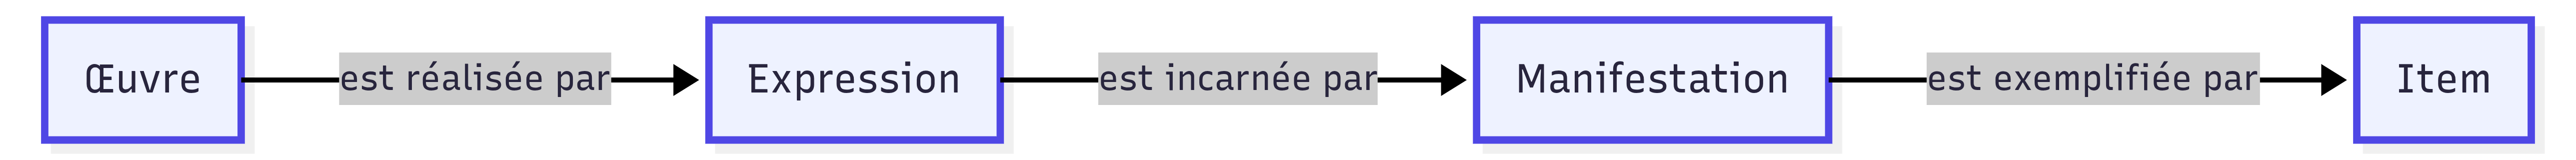
\includegraphics[width=1.0\textwidth]{images/FRBRfirstgroup.png} 
	
	\caption{Entités du modèle \gls{FRBR}} 
	
	\label{figFRBR1} 
	
\end{figure} 



Le \gls{FRBR} est qualifié de modèle entité-relation, qui modélise précisément les relations qui peuvent exister entre les différents niveaux de description et, de ce fait, entre les éléments d'un système d’information, afin de permettre à l'utilisateur de les retrouver plus facilement. Afin d’illustrer la manière dont s’articule la description d’un ouvrage bibliographique selon la modélisation proposée par le FRBR, prenons l'exemple de l'ouvrage \textit{Qu'est-ce que le cinéma} d'André Bazin. Au niveau Œuvre, est décrite l'idée intellectuelle de l'ouvrage, essentiellement matérialisée par son contexte de création. Cet ouvrage, est notamment exprimé et matérialisé au sein d'un texte intégral en quatre volumes écrit entre 1958 et 1962, dont les modalités sont décrites au niveau Expression. Cette expression de l’ouvrage est notamment publiée comme édition originale aux Editions du Cerf, dont les modalités sont décrites au niveau Manifestation. Enfin, l’exemplaire individuel de cette manifestation est potentiellement conservé dans une bibliothèque avec une côte unique, dont les caractéristiques physiques sont décrites au niveau Item. Une même œuvre peut être exprimée au sein de multiples expressions, de même qu’une expression peut faire l'objet de diverses manifestations. Le foisonnement d’éléments liés à une même œuvre peut rapidement rendre complexe la navigation de l’utilisateur au sein d’un outil de gestion des collections. La description proposée par le modèle \gls{FRBR} permet de distinguer les différentes étapes du cycle de vie d’une œuvre et ses différentes matérialisations, permettant ainsi une navigation plus fluide entre les éléments liés au sein d’un catalogue.  

Notons qu’à ces quatre entités de premier groupe Œuvre, Expression, Manifestation, Item), s'ajoutent deux entités de second groupe : Personnes et Collectivités. Elles expriment le rôle joué sur la production ou le contenu d'une ou plusieurs entités du premier groupe. \footcite{zotero-item-657} Par exemple, l'auteur est relié aux niveaux Œuvre et Expression, l'éditeur au niveau Manifestation, le catalogueur au niveau Item. 

Enfin, il existe des entités de troisième groupe intégrées au modèle, qui correspondent à des Concepts, Objets, Évènements ou Lieux liés aux entités de premier et de second groupe. \footcite{zotero-item-657} 

Réunies, les entités des trois groupes confondus modélisent une structure complexe caractérisée par les liens entre éléments, comme le montre la figure \ref{figFRBR2}  

\begin{figure}[htbp] 
	
	\centering 
	
	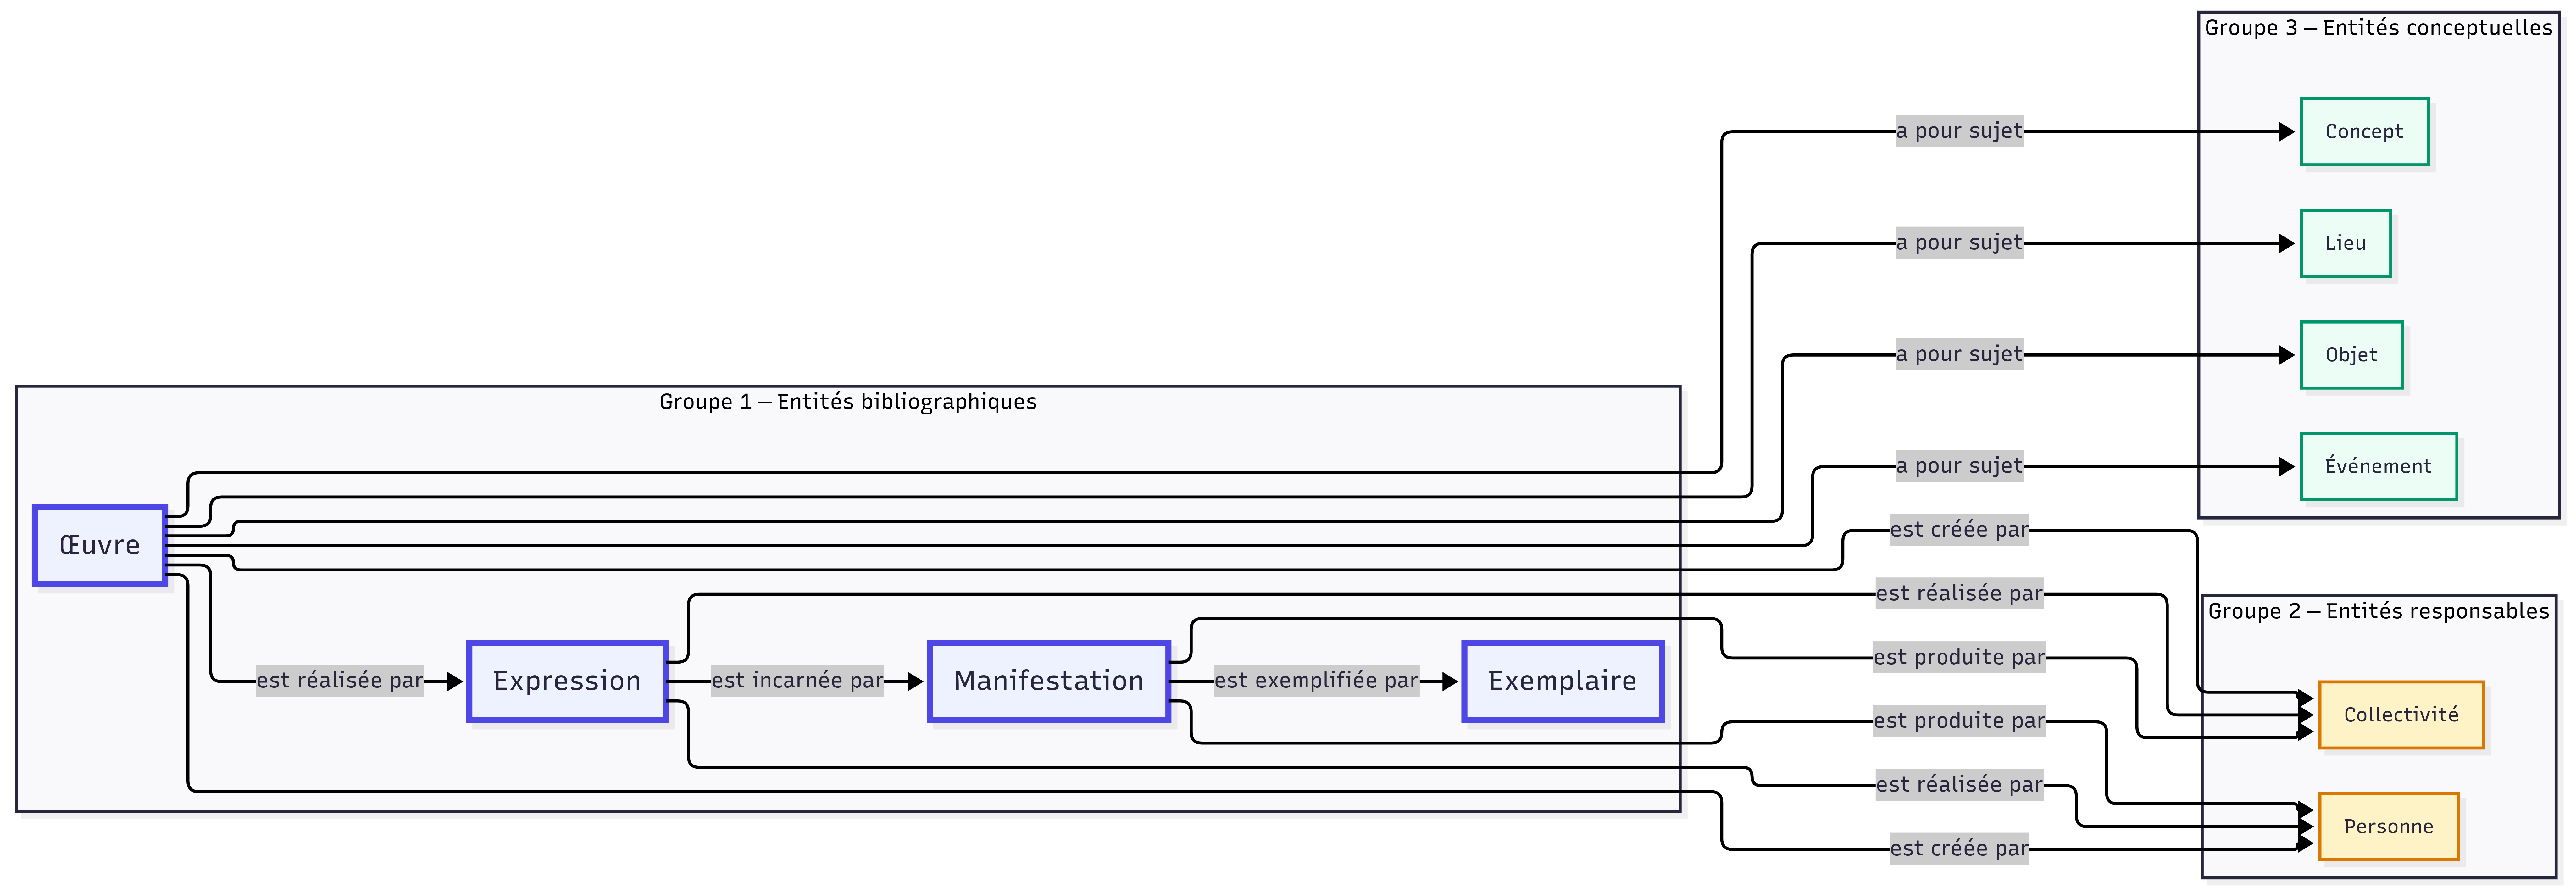
\includegraphics[width=1.0\textwidth]{images/FRBRentitesBiblio.png} 
	
	\caption{Entités du modèle FRBR} 
	
	\label{figFRBR2} 
	
\end{figure} 

Toutefois, dans le cadre de ce mémoire, nous nous concentrerons sur les entités de premier groupe, qui constituent les entités principales de description pour les archives audiovisuelles au sein du logiciel de gestion des collections créé par Skinsoft. Les entités de second et troisième groupe constituent moins des entités à part entière que des éléments de description contrôlés par des thésaurus.  

Le modèle \gls{FRBR}, fondé sur les relations entre entités, est avant tout conçu dans l’optique de faciliter la navigation de l'utilisateur au sein d'un catalogue, entre les liens qui régissent les différents éléments d'une collection.  Le \gls{FRBR} prétend en effet répondre à quatre besoins utilisateur principaux : trouver, identifier, sélectionner, obtenir. \footcite{zotero-item-653}. Il permet à l'utilisateur de localiser la ressource, d'identifier si elle correspond bien à ce qu'il cherche, de la sélectionner selon ses besoins, avant d'accéder finalement à son contenu. Nous ajouterons que le besoin fondateur de la création d'un tel modèle est également celui de pouvoir visualiser et explorer les liens de la ressource identifiée avec d'autres ressources pertinentes qui y sont directement associées. \footcite{zotero-item-653} Ce modèle de données se situerait donc à l'intersection de deux besoins principaux : celui d'améliorer la connaissance sur une ressource donnée en visibilisant ses relations, et celui d'améliorer l'expérience utilisateur en proposant une interface navigable et intuitive. 

%Donner un exemple d’institution qui utilise ce modèle et comment ça se matérialise dans un catalogue en ligne (bibliothèque kandinsky?) 

Notons que ces besoins s'appliquent non seulement à l'utilisateur faisant partie d'un public, au sein d'un catalogue ou d'une base de données en ligne, mais également à un utilisateur métier, interne à l'institution et gestionnaire des collections. C'est précisément sur les besoins métier de ce dernier que se concentre l'analyse de ce mémoire de recherche, puisque Skinsoft propose avant tout un outil de gestion des collections interne. De fait, les enjeux de l'implémentation et de l'adaptation du modèle \gls{FRBR} se situent au cœur des ambitions d'un logiciel de gestion des collections, dont l’objectif est d’améliorer l’interface afin d’assurer l’efficacité de l’utilisateur métier.  







%L'adoption de ces modèles dans les catalogues est réalisé dans l'objectif d'améliorer la visibilité des données au sein du web de données et donner accès au public aux données produites, même si ce mémoire se concentre sur l'utilisateur métier. (définir le web de données?) \footcite{zotero-item-661} 


\subsubsection{Son adaptation à l'archivistique et au contexte muséal}

Le modèle \gls{FRBR} est un modèle conçu par et pour les bibliothèques. À ce jour, les bibliothèques n'utilisent plus seulement le modèle FRBR mais la somme du FRBR et de ses modèles étendus : le \gls{FRAD} (Fonctionnalités requises des données d'autorité) pour la description des autorités, et le FRSAD (Fonctionnalités requises des données d'autorité matière) pour la description des sujets.\footcite{zotero-item-651}. La somme de ces modèles constitue le modèle \gls{IFLA-LRM}, successeur du \gls{FRBR}. Le modèle \gls{FRBR} est toutefois largement utilisé dans le domaine de la gestion des collections muséales. Or, sa qualité de modèle ne prétend pas normaliser la description des données, seulement d’en cadrer l’affichage. De fait, les entités proposées par le modèle \gls{FRBR} peuvent paraître génériques, et doivent être soumises à une redéfinition à chaque implémentation selon le contexte donné \footcite{boeuf2008}. Cette flexibilité ne doit toutefois pas nuire à l'objectif principal, celui de faciliter la navigation de l'utilisateur, en explicitant les “interrelations" entres les notices et les données produites \footcite{boeuf2008}. Nous étudierons dans les chapitres suivants une double adaptation, celle du modèle \gls{FRBR} à d’autres types de documents : objets de collections et archives, et son adaptation à différents contextes institutionnels pour une même nature de documents, celle des archives audiovisuelles.  

%Analysons premièrement son adaptation au milieu archivistique. La difficulté principale de l'adaptation du modèle FRBR aux collections d'archives est que le niveau Œuvre ne peut contenir le plus haut niveau archivistique : le fonds d'archives. En effet, un fonds d'archive ne peut être considéré systématiquement comme une œuvre, puisque dans la plupart des cas, il s'agit plutôt d'une agrégation naturelle d'éléments quotidiens produits par une personne morale ou physique. Ainsi, un fonds d'archives ne peut être intégré à la définition d'une œuvre comme création intellectuelle et artistique distincte \footcite{fick2015}. Un fonds d'archives correspondrait davantage à un agrégat d'œuvres ou de travaux, niveau intermédiaire décrit par le modèle FRBR : "un ensemble de documents privés classés par des archives en un seul fonds"(traduction). \footcite{fick2015}. Le niveau manifestation est obsolète car les archives ne sont pas publiées ?  

%Développer un peu plus sur l’adaptation du modèle aux archives : qu’en est-il des autres niveaux ? À quoi ressemble un catalogue d’une institution qui utilise le FRBR pour les archives ? (À relier avec le sujet) 

Le modèle de données \gls{FRBR} a été adapté au milieu muséal à travers une version orientée objet, le \gls{FRBRoo}, extension du \gls{CIDOC-CRM} (object-oriented Conceptual Reference Model), l'ontologie de référence dédiée au patrimoine culturel et muséal \footcite{gillis2015}. Il s’agit d’un modèle conceptuel général visant l’interopérabilité entre les données provenant d’institutions diverses dont les musées, centres d’archives et bibliothèques.  

Ce dernier modélise une approche descriptive centrée sur les évènements entourant l’objet décrit. Ainsi, les entités bibliographiques ne sont plus seulement décrites par des attributs, mais par des évènements spatio-temporels qui les créent et les font évoluer selon différents contextes \footcite{dialogue2017} Cette adaptation du \gls{FRBR} est particulièrement pertinente pour la description de collections de musées composites et de différentes natures, pouvant englober à la fois la description de tableaux, sculptures, ouvrages, specimens, films, etc. Tandis que le \gls{FRBR} est modélisé à partir de la nature d’un document bibliographique le FRBRoo replace la description dans un contexte plus large, celui d’évènements situés dans l’espace et dans le temps, évènements qui peuvent agir sur n’importe quel type d’objet.  

Le \gls{FRBRoo} est un modèle intéressant pour la gestion des archives audiovisuelles. En effet, les \gls{Archivesaudiovisuelles} possèdent un statut hybride au sein d’institutions patrimoniales, relevant à la fois de la création artistique, de l’œuvre et d’un archivage du réel, d’un témoignage \footcite{zotero-item-669}. Le \gls{FRBRoo} propose deux entités pertinentes, qui pourraient permettre de distinguer l’évolution de ce double statut : l’œuvre (Individual work), et la captation ou l’enregistrement (Recording work). Par exemple, l’étape du tournage serait documentée par l’entité Captation ainsi que l'ensemble des évènements et des personnes qui y sont liés, alors que le montage serait documenté par l’entité Œuvre ainsi que les évènements et les personnes qui y sont liés. Le FRBRoo conserve ensuite les entités prévues par le FRBR : l’Expression, la Manifestation, l’Item.  

Néanmoins, si le FRBRoo constitue une adaptation pertinente du FRBR pour le milieu muséal, sa structure trop large ne permet pas de rendre compte la nature propre du médium cinématographique, qui fonde la gestion des collections audiovisuelles. Ainsi, les institutions préservatrices de collections audiovisuelles se tournent davantage vers des adaptations métier spécifiques, comme celle de la fédération des archives du film (FIAF). La FIAF propose en effet une application du FRBR spécifique aux usages métier de description des archives audiovisuelles, au sein d’un manuel de catalogage des images animées. 



\subsubsection{Un modèle adapté aux archives audiovisuelles : le manuel de catalogage des images animées de la FIAF } 

L’adaptation du modèle FRBR aux archives audiovisuelles impose une double redéfinition : elle doit prendre en compte d’une part la nature propre du langage cinématographique, et d’autre part, les spécificités des corpus audiovisuels conservés. La modélisation en différentes couches de description prévue par le FRBR est pertinente pour le cinéma, qui partage avec le milieu bibliographique un mode de production industriel, permettant ainsi de distinguer la création intellectuelle de ses copies et diffusions multiples. Toutefois, les niveaux bibliographiques classiques dits WEMI (Work, Expression, Manifestation, Item) restent limitées pour la description métier des spécificités des archives audiovisuelles.  

Premièrement, alors que les bibliothèques conservent principalement des copies identiques d’une même publication, les archives d’images animées sont fréquemment amenées à gérer des objets uniques et rares tels que des \textit{rushes}, des films amateurs, montages inachevés, copies annotées, etc. \footcite{zotero-item-646}. Pour ce type de collections, le niveau Manifestation devient obsolète, en raison du caractère inédit de leur création. Deuxièmement, la distinction du FRBR bibliographique entre l’Œuvre (l’idée de création), et l’Expression (sa réalisation) s’adapte mal au contexte cinématographique. En effet, un film prend véritablement forme au moment du tournage puis du montage, rendant ainsi l’idée d’une existence abstraite de création en amont, caduque. Il parait alors plus pertinent d’appréhender l’œuvre cinématographique moins comme une entité abstraite en amont de son expression que comme une entité concrète ancrée dans un processus d’expression.  

Afin de répondre à ces contraintes imposées par le processus de création cinématographique, la FIAF a élaboré un manuel de catalogage des images animées \footcite{zotero-item-644}. Le manuel adapte le modèle FRBR en le combinant aux règles descriptives RDA (Ressources, Description, Accès) dédiées aux archives, et aux normes de description des œuvres cinématographiques (EN 15744 / EN 15907) \footcite{zotero-item-646}. Le manuel se focalise sur les entités de premier groupe afin d’en repenser l’articulation et de proposer de remplacer le schéma WEMI par le schéma WVMI (Work, Variant, Manifestation, Item).  

En effet la FIAF propose de fusionner le niveau Expression dans celui de l'Œuvre, permettant alors à l’Œuvre de regrouper la description intellectuelle et le processus de création de l’archive cinématographique. Par exemple, si nous prenons le film \textit{L'Aigle à deux têtes} (France, 1948, réalisé par Jean Cocteau), le niveau Oeuvre permettrait d’y décrire le contexte de création ainsi que le contenu. De plus, la FIAF propose une nouvelle entité, celle de Variante, optionnelle, qui se substitue à celle d’Expression. Elle permet de décrire toute version différente d’une œuvre originale dans la mesure où son sens principal n’est pas altéré. Par exemple, une version d’un film qui serait colorisée, censurée, doublée, remontée, etc. Si nous reprenons \textit{L'Aigle à deux têtes}, une variante possible est celle de la restauration du film en 4K en 2023, dont le niveau Variante permettrait de décrire les variations portées sur l’œuvre. La FIAF conserve par ailleurs le niveau de Manifestation, toutefois redéfini afin de pouvoir décrire la matérialisation physique ou numérique d’une Œuvre ou de sa Variante sur un support, ainsi que son contexte de diffusion. Par exemple, la manifestation de la version restaurée de \textit{L'Aigle à deux têtes} décrirait la sortie de cette version en Blu-Ray et DVD chez Rimini Editions. Enfin, le niveau Item est également conservé afin de décrire l’exemplaire physique ou le fichier numérique unique issu de la Manifestation d’une Œuvre ou de sa Variante. Cet exemplaire est concrètement préservé et géré par l’institution et décrit par des métadonnées de conservation.  
		
		Cette restructuration du FRBR permet ainsi de répondre aux besoins métiers spécifiques de gestion de collections d’images animées. Selon la FIAF, la modélisation de cette réadaptation du FRBR au sein d’un outil de gestion des collections devrait permettre aux utilisateurs métier “d’identifier, sélectionner et acquérir” efficacement toutes les variantes d’une œuvre, l’ensemble des manifestations d’une version d’une œuvre, les exemplaires physiques disponibles d’une manifestation d’une œuvre \footcite{zotero-item-646}. La FIAF reprend ainsi les besoins utilisateurs fondateurs de la structuration du FRBR bibliographique en les adaptant à une nécessité de pouvoir circuler entre les différentes versions d’une œuvre à différents stades du processus de l’industrie cinématographique.  
		
		Toutefois, l’implémentation d’un tel modèle au sein d’un outil de gestion des collections se heurte aux spécificités des différents corpus audiovisuels, dont certains ne possèdent pas de manifestation par exemple. En effet, si le modèle s'applique adéquatement aux corpus de cinéma dits "classiques" dont la chaîne de production industrielle est respectée : un film est réalisé à l'issue d'un tournage et d'un montage (Œuvre), puis distribué (Manifestation), et copié en multiples exemplaires (Item). Or, dans le cas de corpus spécifiques, expérimentaux, personnels, ou amateurs, qui font l’objet de descriptions complexes, la modélisation FRBR classique s'avère limitée. Ce type de corpus est notamment peu distribué ou diffusé, rendant notamment le niveau de Manifestation obsolète. 
		
		Ainsi, le FRBR reste un modèle qu’il s’agit de réadapter à chaque contexte institutionnel \footcite{boeuf2008}. Le manuel de la FIAF agit comme un cadre théorique de structuration de la description pour la globalité des archives audiovisuelles, qui subit une redéfinition pour chaque type de corpus audiovisuel : amateur, commercial, documentaire, grand public, etc.  
		
		Reproductibilité technique ? \footcite{zotero-item-669} 
		
		
		
		%le but ultime de la modélisation des données et de leur structuration est leur interopérabilité et leur versement sur le web de données par les institutions qui le souhaitent. Permet de passer de la donnée brute à l'information intelligible. dès l'inventaire des données, la modélisation doit être prise en compte et également le multilinguisime pour faciliter l'ouverture des données. \footcite{chambonnet} 
		
		%Nécessité d'uniformiser même si les corpus sont hétérogènes pour assurer l'intéropérabilité des données.  
		
		%Transition vers la deuxième sous partie : adapter le FRBR aux archives audiovisuelles 
		
		
		
		%à replacer - fin de la deuxième sous partie :  
		
		%Transition entre le modèle de données et l'automatisation :  
		
		%justification de la clarté du modèle FRBR pour la mise en place d'un modèle automatique :  
		
		% 
		
		%Impact de l'indexation automatique sur les données : 
		
		% 
		
		%"Comme le repérage d’entités visuelles demande énormément d’informations locales, les bases de données d’indexation constituées à partir de la reconnaissance des entités sont conséquentes (elles peuvent avoir une taille supérieure à celle des vidéos elles-mêmes) et font l’objet de recherches au sein de l’établissement pour en optimiser les temps de calcul. Dans ce contexte, la qualité et la modélisation des données jouent un rôle fondamental car c’est sur les bases de données que les algorithmes sont entrainés."\footcite{moiraghi2018} 
		
		% 
		
		%Nous prenons ici la pensée inverse, ce n'est pas seulement l'indexation automatique qui nécessite un modèle de données qualitatif, mais nous réfléchissons justement à la manière dont le modèle de données façonne l'indexation automatique et la manière dont l'indexation automatique permet de repenser le modèle de données dans lequel est implémentée.  
		
		% 


%	\subsection{Implémenter le FRBR adapté aux archives audiovisuelles au sein d’un outil de gestion des collections} 

%I 2 

%Reprendre la définition du logiciel de gestion des collections ? Pour montrer que le FRBR aide à la gestion des collections 

Comme défini en introduction, un logiciel de gestion des collections est un outil “spécialisé permettant de gérer des informations structurées” \footcite{zotero-item-766}. De ce fait, il structure le système d’information qui permet à une institution d’orchestrer le cycle de vie de sa collection. Cette structuration des données doit être modélisée selon les spécificités propres au type de collection d’un institution cliente, à partir de normes descriptives définies et de cadres de référence pour l’indexation des collections. Dans le cas des archives audiovisuelles, le logiciel des gestions des collections devrait ainsi permettre une structuration de l’information adaptée au type de corpus conservé, respectant toutefois le cadre de référence pour la modélisation des données, le FRBR. La restructuration du modèle de données permet de construire pour l’utilisateur, un logiciel de gestion des collections intelligible avec des outils de recherche performants. (En accord avec les besoins utilisateurs FRBR)  


\subsubsection{Un espace de travail dédié à la gestion de collections audiovisuelles : S-Movies}

Si le manuel de la FIAF pose le cadre d’une adaptation du modèle FRBR pour la gestion des archives audiovisuelles, il s'agit désormais de confronter ce cadre à une implémentation concrète. Pour cela, nous analyserons au cours de ce chapitre l’implémentation d’une telle modélisation au sein d’un outil de gestion des collections, celui développé par Skinsoft. Nous y analyserons spécifiquement l’espace de travail développé pour la gestion des archives audiovisuelles : S-Movies. En effet, le contexte de notre étude se situe principalement dans le cadre de l’analyse de cet espace de travail afin d’en analyser la modélisation, en vue de l’améliorer et d’y implémenter potentiellement des fonctionnalités automatiques, fondées sur l’intelligence artificielle.  

Présentons d’abord le fonctionnement général de l’outil de gestion des collections développée par Skinsoft. Celui-ci est divisé en espaces de travail, chacun dédiés à un type de collection, comme le montre la capture d'écran de la page d'accueil ci-dessous (\ref{figAccueil}). (dire en note de bas de page que les captures viennent d’une appli de test configurée par nos soins)

\begin{figure}[htbp] 
	
	\centering 
	
	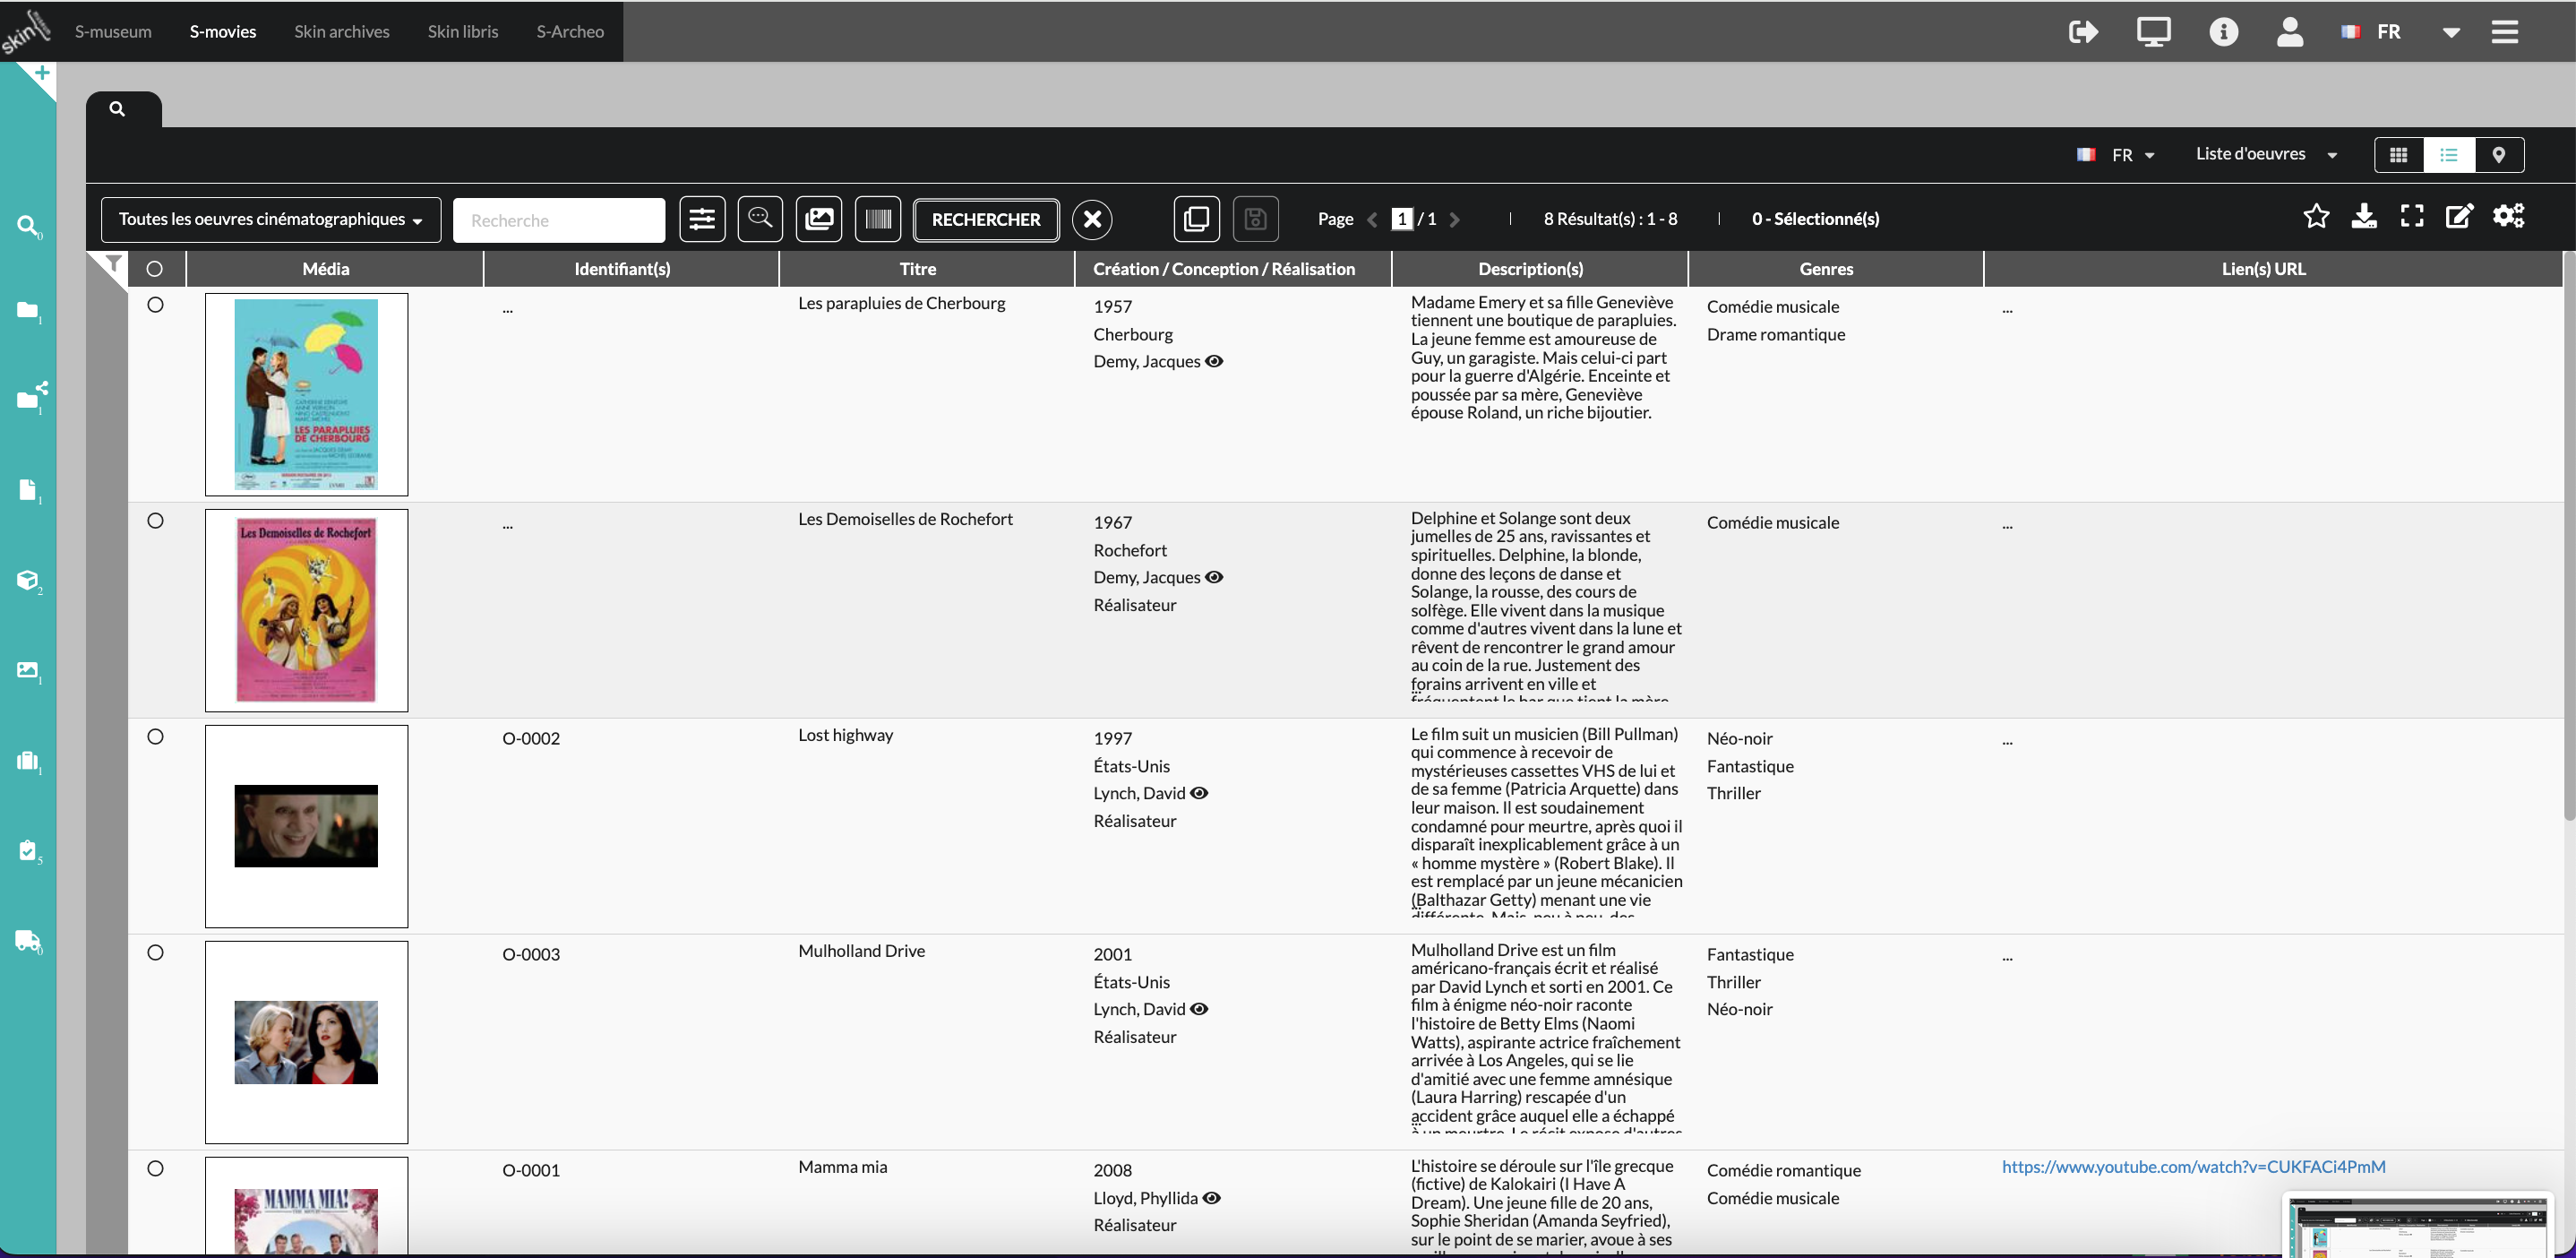
\includegraphics[width=0.85\textwidth]{images/image.png} 
	
	\caption{Page d'accueil de l'espace de travail} 
	
	\label{figAccueil} 
	
\end{figure}

Une institution cliente de l’outil peut combiner un ou plusieurs espaces de travail, selon les données à gérer. Cette structure permet justement d’adapter l’interface à chaque type de collection géré : objets de collection de musée, collections archéologiques, collections de films, collections bibliographiques, collections d’archives, etc. Chaque espace de travail permet notamment la gestion des acquisitions, des collections, de leurs mouvements, de projets, d’expositions, des médias... De plus, chaque espace de travail est structuré selon des normes de description et un cadre de modélisation adaptés au type de collection qui y est géré. L'espace de travail S-Movies est modélisé selon les préconisations de la FIAF sur l’adaptation du FRBR, et structuré selon les normes de descriptions évoquées. Ainsi, les collections sont organisées en trois entités distinctes, conformément aux adaptations du FRBR par la FIAF : Films, Manifestations, Œuvres cinématographiques (Films désigne ici le niveau Item), comme le montre la capture d'écran du menu de l'espace de travail, ci-dessous :   

\begin{figure}[htbp] 
	
	\centering 
	
	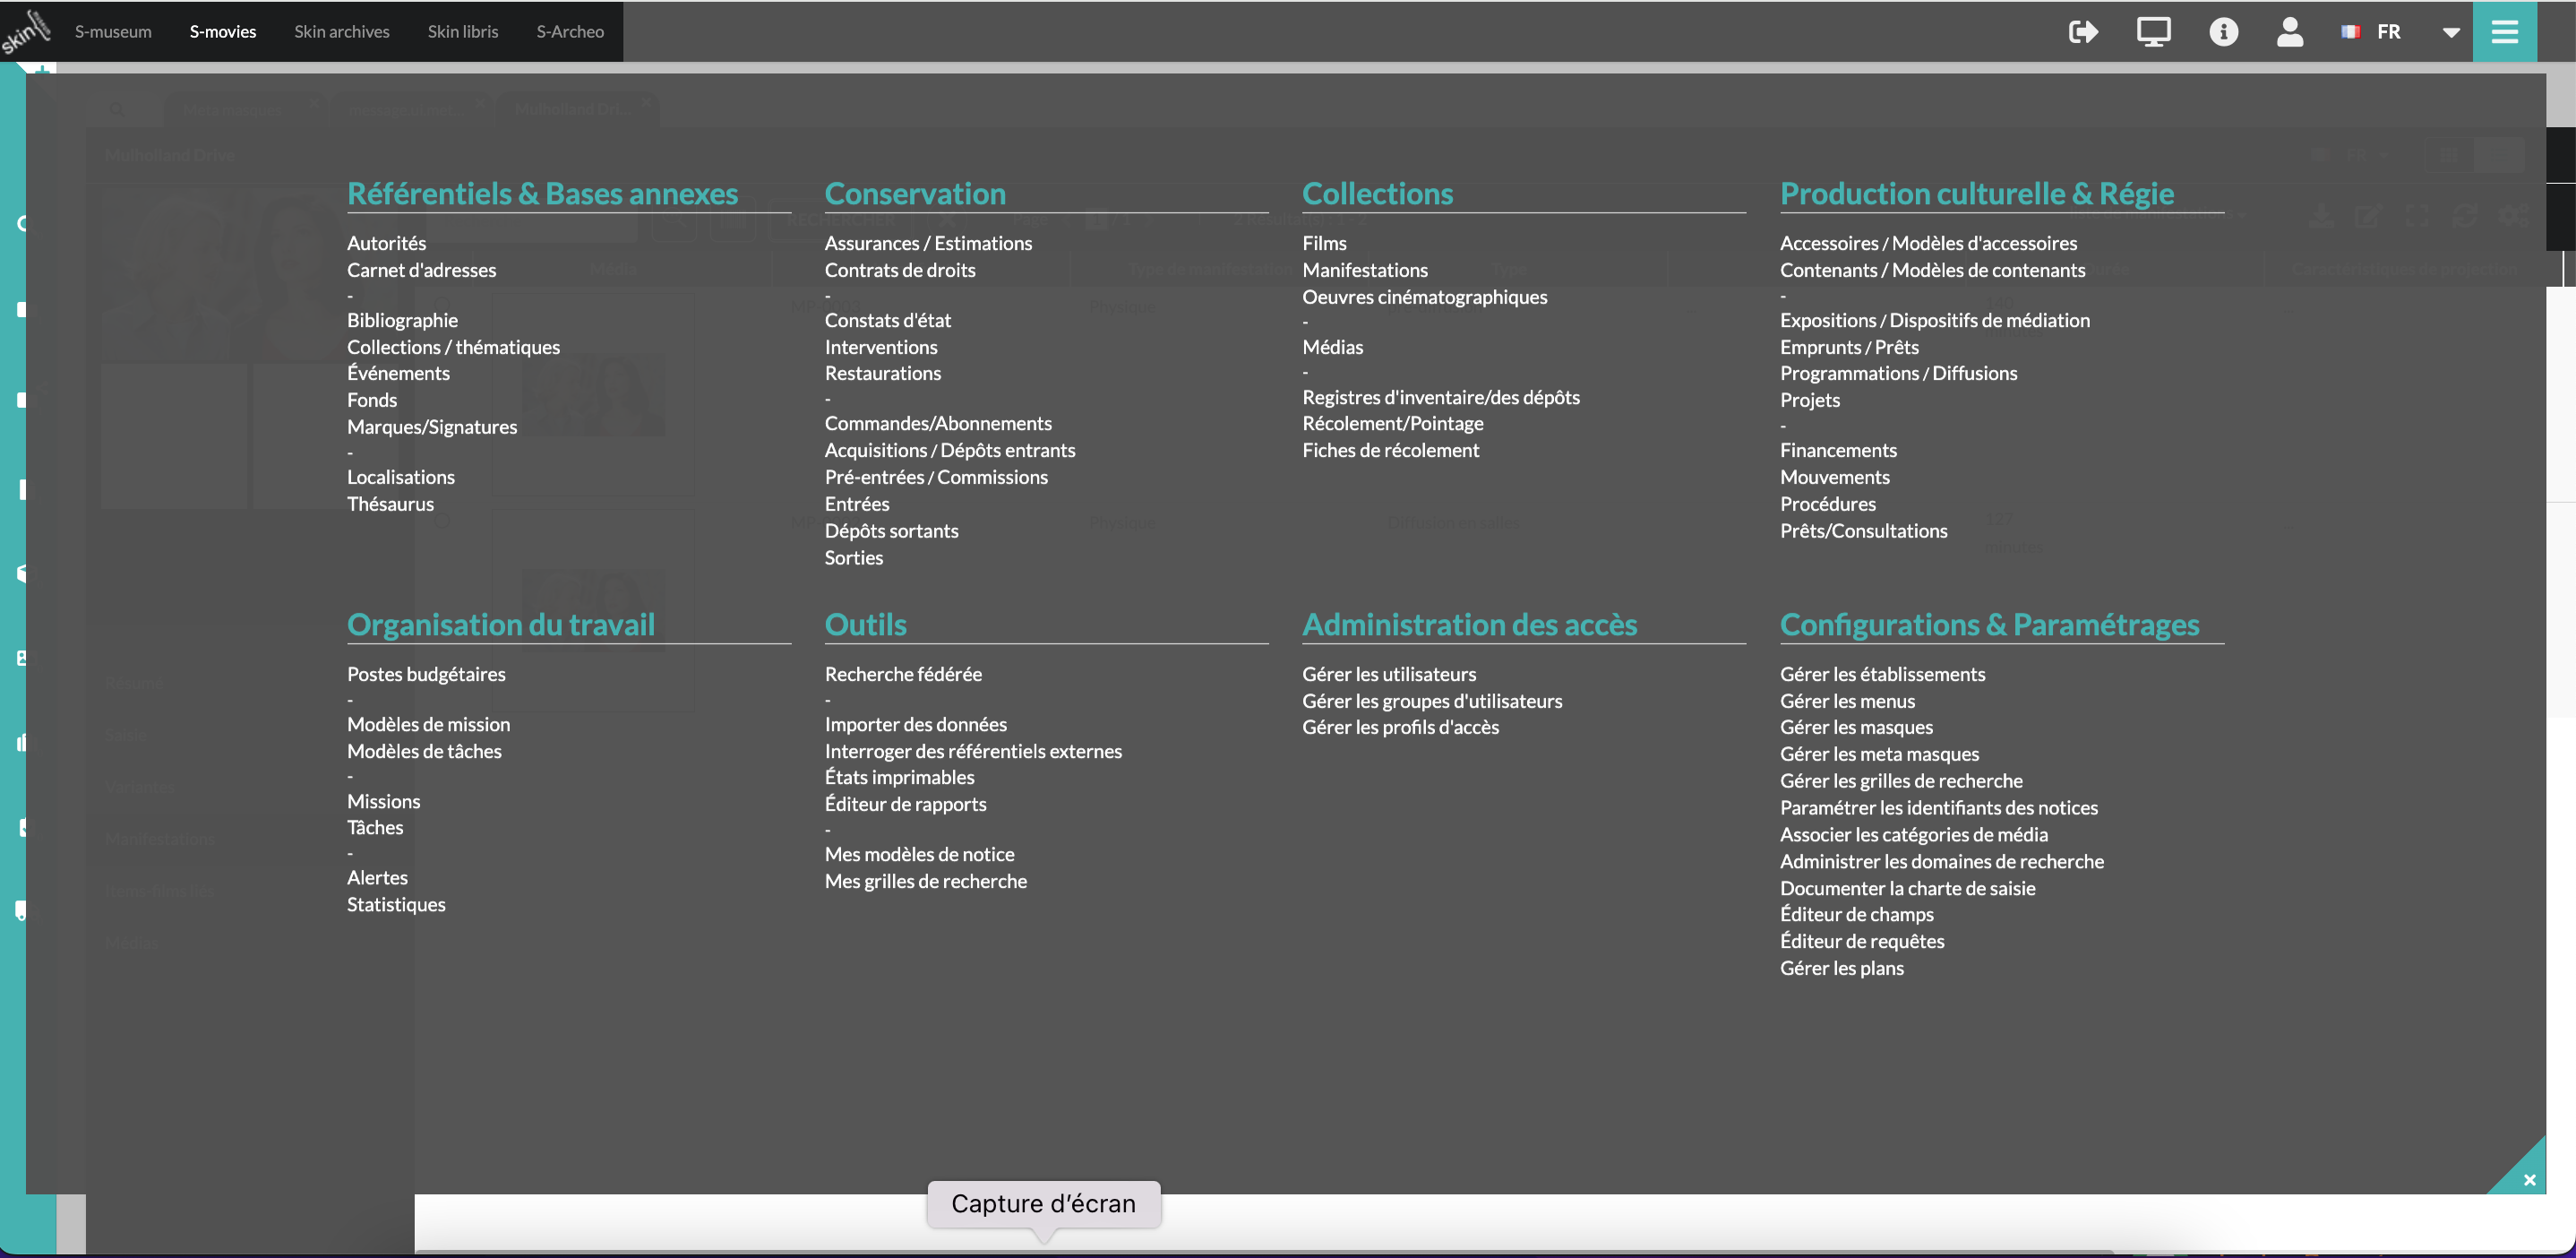
\includegraphics[width=0.85\textwidth]{images/image6.png} 
	
	\caption{Menu burger de l'espace de travail} 
	
	\label{figMenu} 
	
\end{figure}

Dans chacune de ces tables de données, l'utilisateur peut créer de nouvelles notices, et y associer des notices des autres tables. Par exemple, depuis la table Œuvres cinématographiques, l'utilisateur peut créer une notice d’Œuvre et y associer des notices de Manifestations et d'Items qui y sont directement liées. La Variante telle que définie dans le manuel de la FIAF n’est pas représentée par une entité à part entière sous la forme d’une table comme c’est le cas pour les autres entités. Toutefois, il est possible de créer une notice de Variante au sein de la table Œuvres cinématographiques, directement liée à une Œuvre. La Variante aura le même statut qu’une Oeuvre, mais elle sera de type Variante.  

Par exemple ci-dessous, une notice d’Œuvre cinématographique à laquelle sont associées deux notices de Manifestation :  

\begin{figure}[htbp] 
	
	\centering 
	
	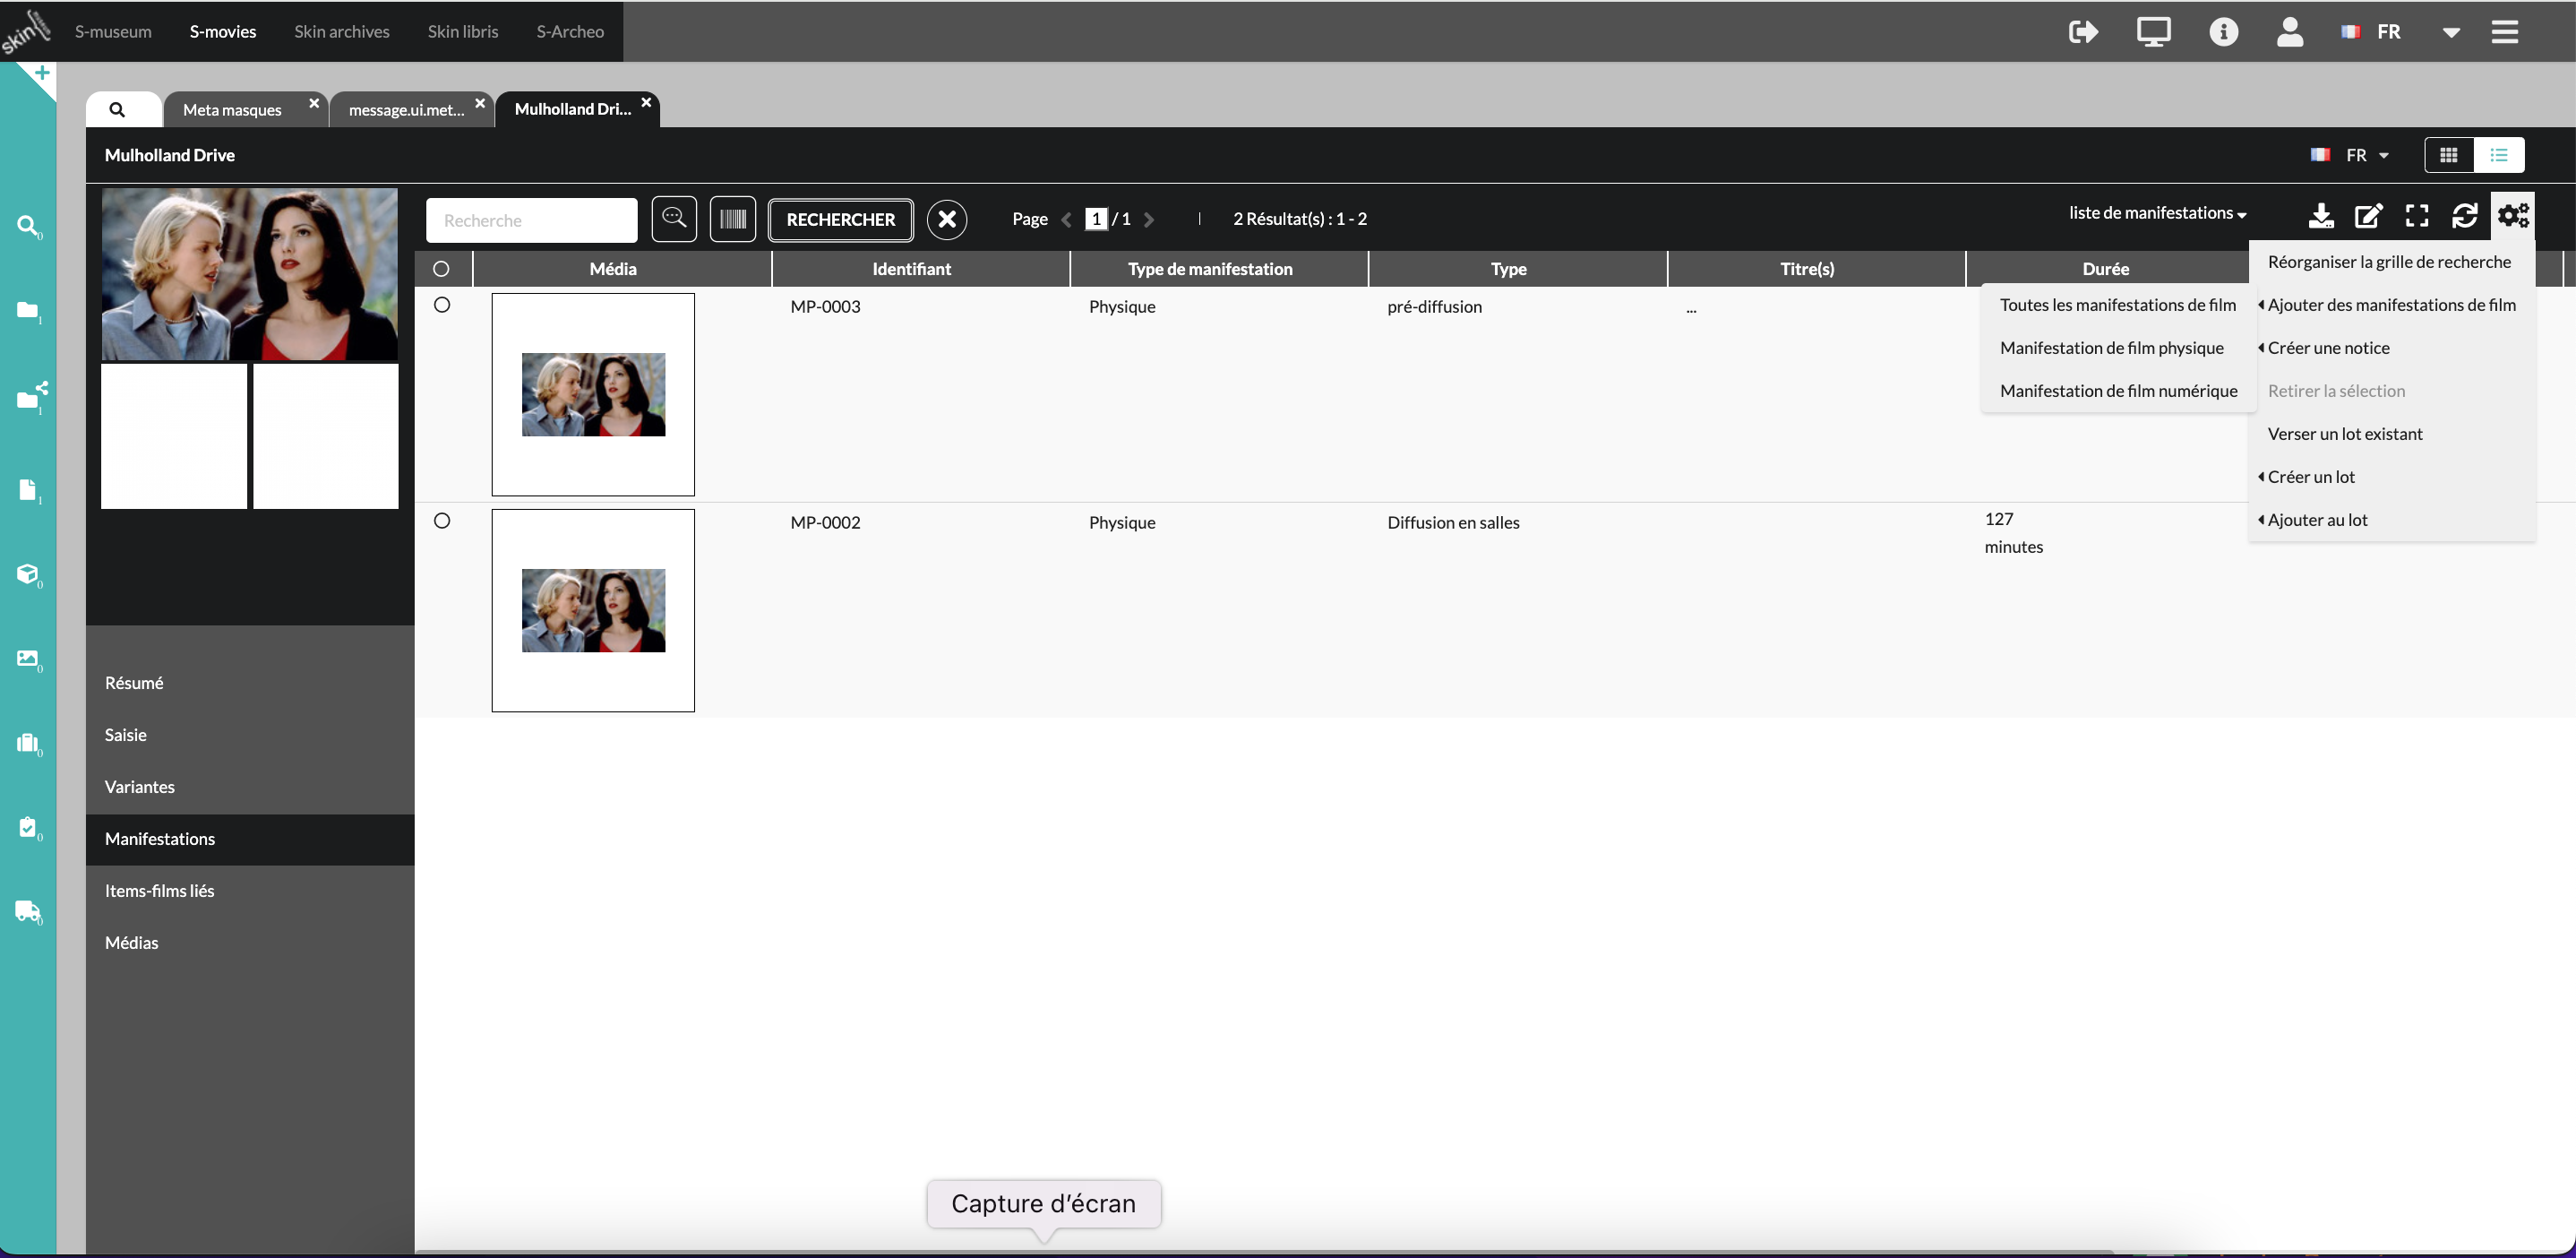
\includegraphics[width=1.0\textwidth]{images/image7.png} 
	
	\caption{Menu burger de l'espace de travail} 
	
	\label{figNoticeOeuvre} 
	
\end{figure}

L’interface permet d’associer des notices depuis un bouton d’action situé à droite.  

De plus, en fonction de la nature du corpus géré, un paramétrage adaptatif est prévu afin d’ajuster l’interface aux pratiques métier de chaque institution. En effet, une adaptation supplémentaire de la modélisation de données via la configuration flexible de chacun des espaces de travail. Trois configurations sont principalement possibles : le paramétrage de champs de saisie pour chaque type de notice, l'organisation de ces champs dans des grilles de résultats de recherche, et l'assemblage des champs et des grilles de recherche dans des menus navigables pour chaque type de notice. (Schémas explicatifs ?) Ce paramétrage concrétise la modélisation de données selon le cadre de référence utilisé.  

%quel rôle joue la modélisation dans ce cas ? En amont du paramétrage ? Ou en aval ? (Reprendre la définition) ou tout ce paramétrage fait partie de la modélisation  

Ainsi, une double adaptabilité est proposée : d’une part un espace dédié à un type de collection et structuré en fonction des normes de description et de la modélisation de données préférée, et d’autre part un paramétrage précis de l’espace de travail, propre au type de corpus géré par l'institution cliente, concrétisant ainsi la modélisation de données propre qui sera utilisée.  

L’espace de travail S-Movies est pré structuré suivant la modélisation FRBR préconisée par la FIAF. Cette structure stable, permet à Skinsoft de proposer un espace de travail pré défini pour chaque institution préservatrice de ce type de collection. En revanche, les corpus audiovisuels préservés par différentes institutions peuvent être de toutes sortes, sur différentes thématiques, sous différents formats. Cette hétérogénéité suppose des règles métiers spécifiques, issues des besoins de gestion de la collection préservé. Ainsi, par exemple, une collection audiovisuelle expérimentale ou amateure ne nécessitera pas les mêmes champs de saisie, les mêmes thésaurus, ou de la même disposition des résultats de recherche, qu'une collection audiovisuelle industrielle, grand public.   

Concrètement, au sein de l’espace de travail, la description d’un élément s’effectue au sein de champs de saisie, sélectionnés de manière adaptée aux besoins de description de l’institution donnée. Ces champs, s'ils sont paramétrables individuellement, font en réalité partie d'une structure plus large, à l'échelle de l'espace de travail dans lequel ils se situent. En effet, ces champs sont regroupés dans des masques, qui correspondent à des formulaires de saisie spécifiques au type de notice concerné. Par exemple, une notice de film physique, décrivant le niveau Item pourra contenir un masque de saisie, contenant des champs de saisie correspondants (cf \ref{figMasques}): identifiants, format de l’item, support de l’item, etc. 

\begin{figure}[htbp] 
	
	\centering 
	
	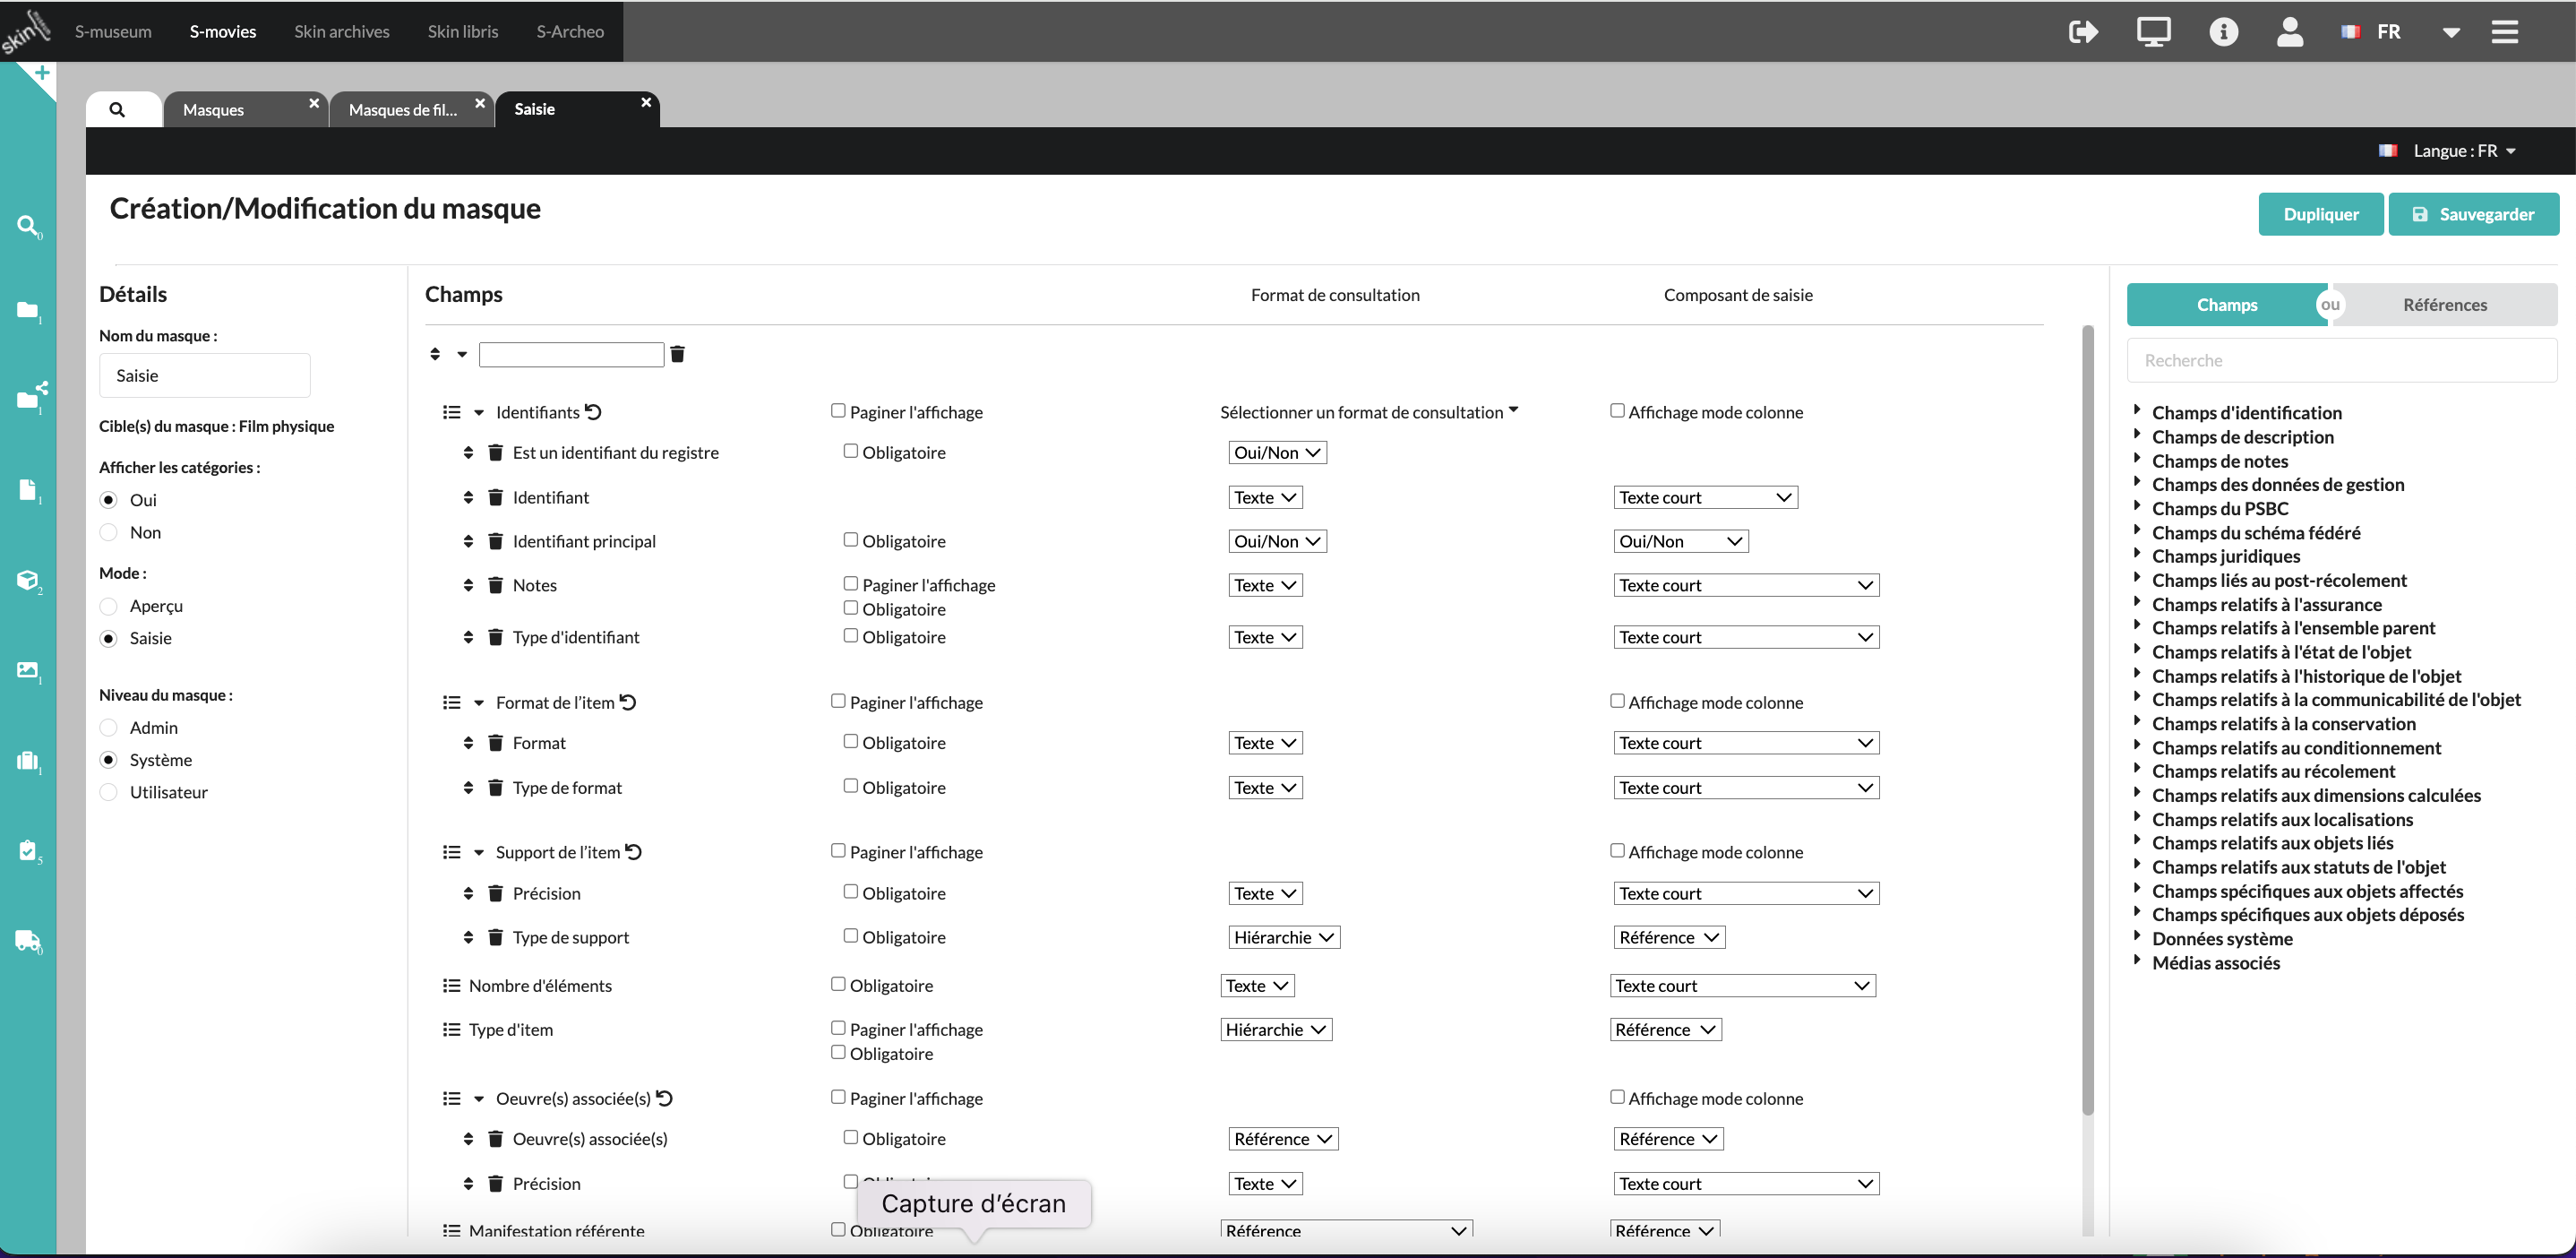
\includegraphics[width=1.0\textwidth]{images/image2.png} 
	
	\caption{Configuration des masques de saisie au niveau Item} 
	
	\label{figMasques} 
	
\end{figure}

Ce masque pourra ensuite être assemblé en tant qu’onglet au sein d’un menu d'une notice de film physique, permettant à l'utilisateur d'y remplir les champs que nous avons mentionnés. Ici, le menu d’une notice de film physique qui contient le masque de saisie mentionné plus haut :  

\begin{figure}[htbp] 
	
	\centering 
	
	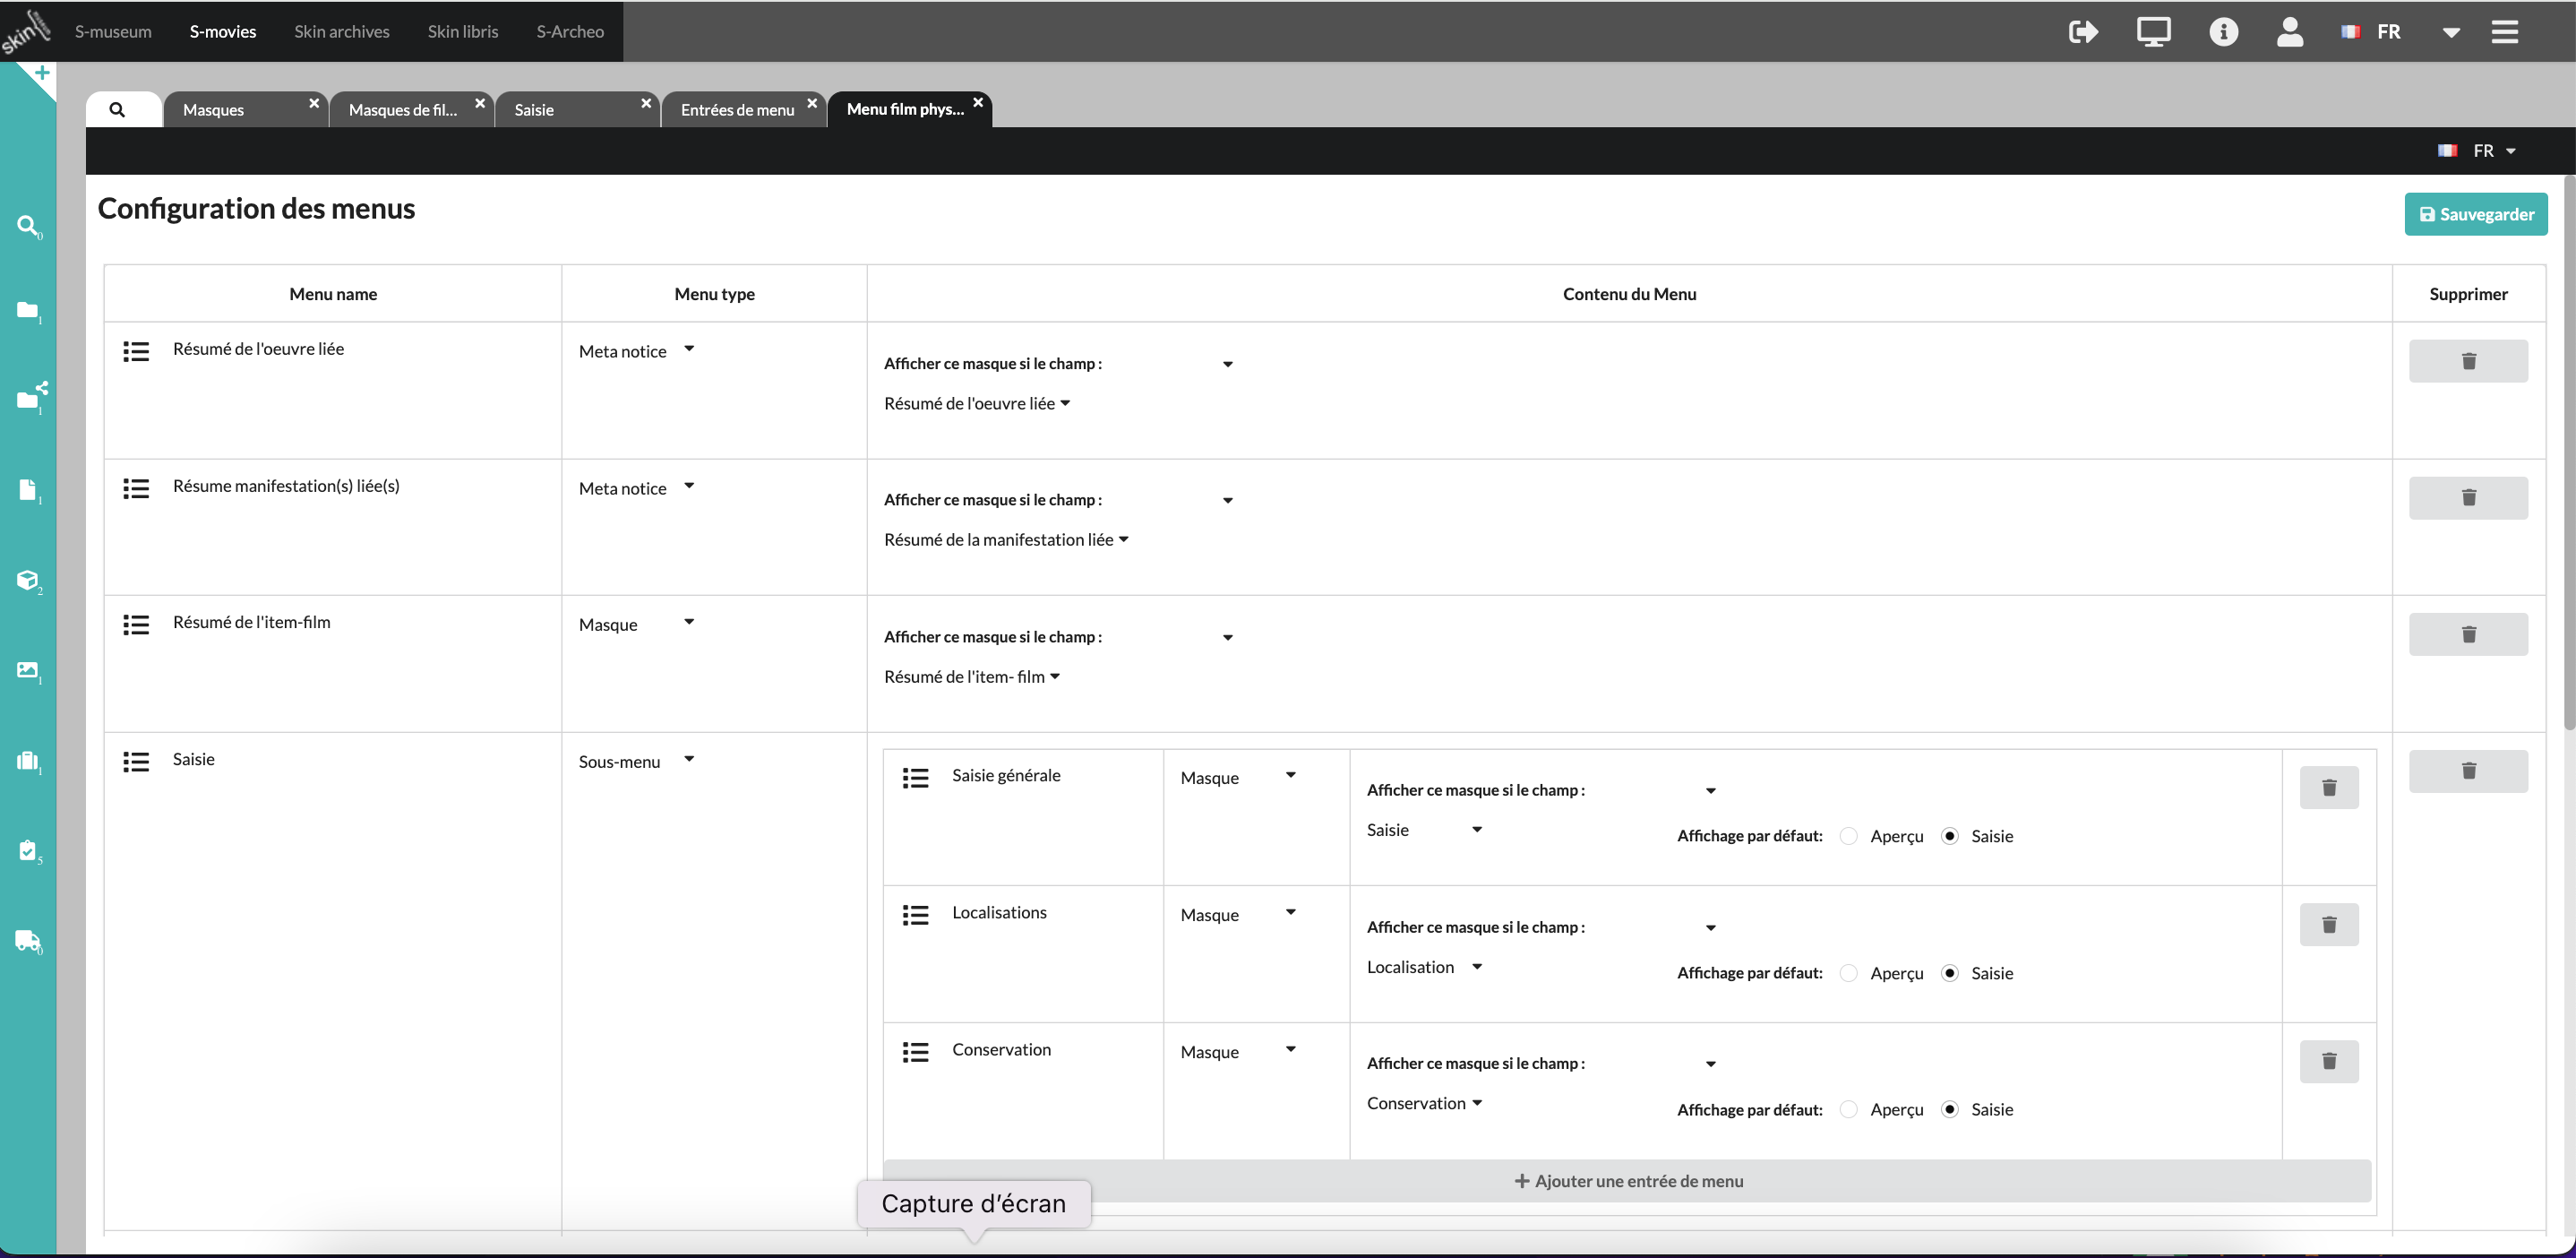
\includegraphics[width=1.0\textwidth]{images/image3.png} 
	
	\caption{Configuration du menu d'une notice de film physique} 
	
	\label{figMenuFilm} 
	
\end{figure}

Et ici la manière dont il s’affiche pour l’utilisateur, à la saisie dans une nouvelle notice de film physique :  

\begin{figure}[htbp] 
	
	\centering 
	
	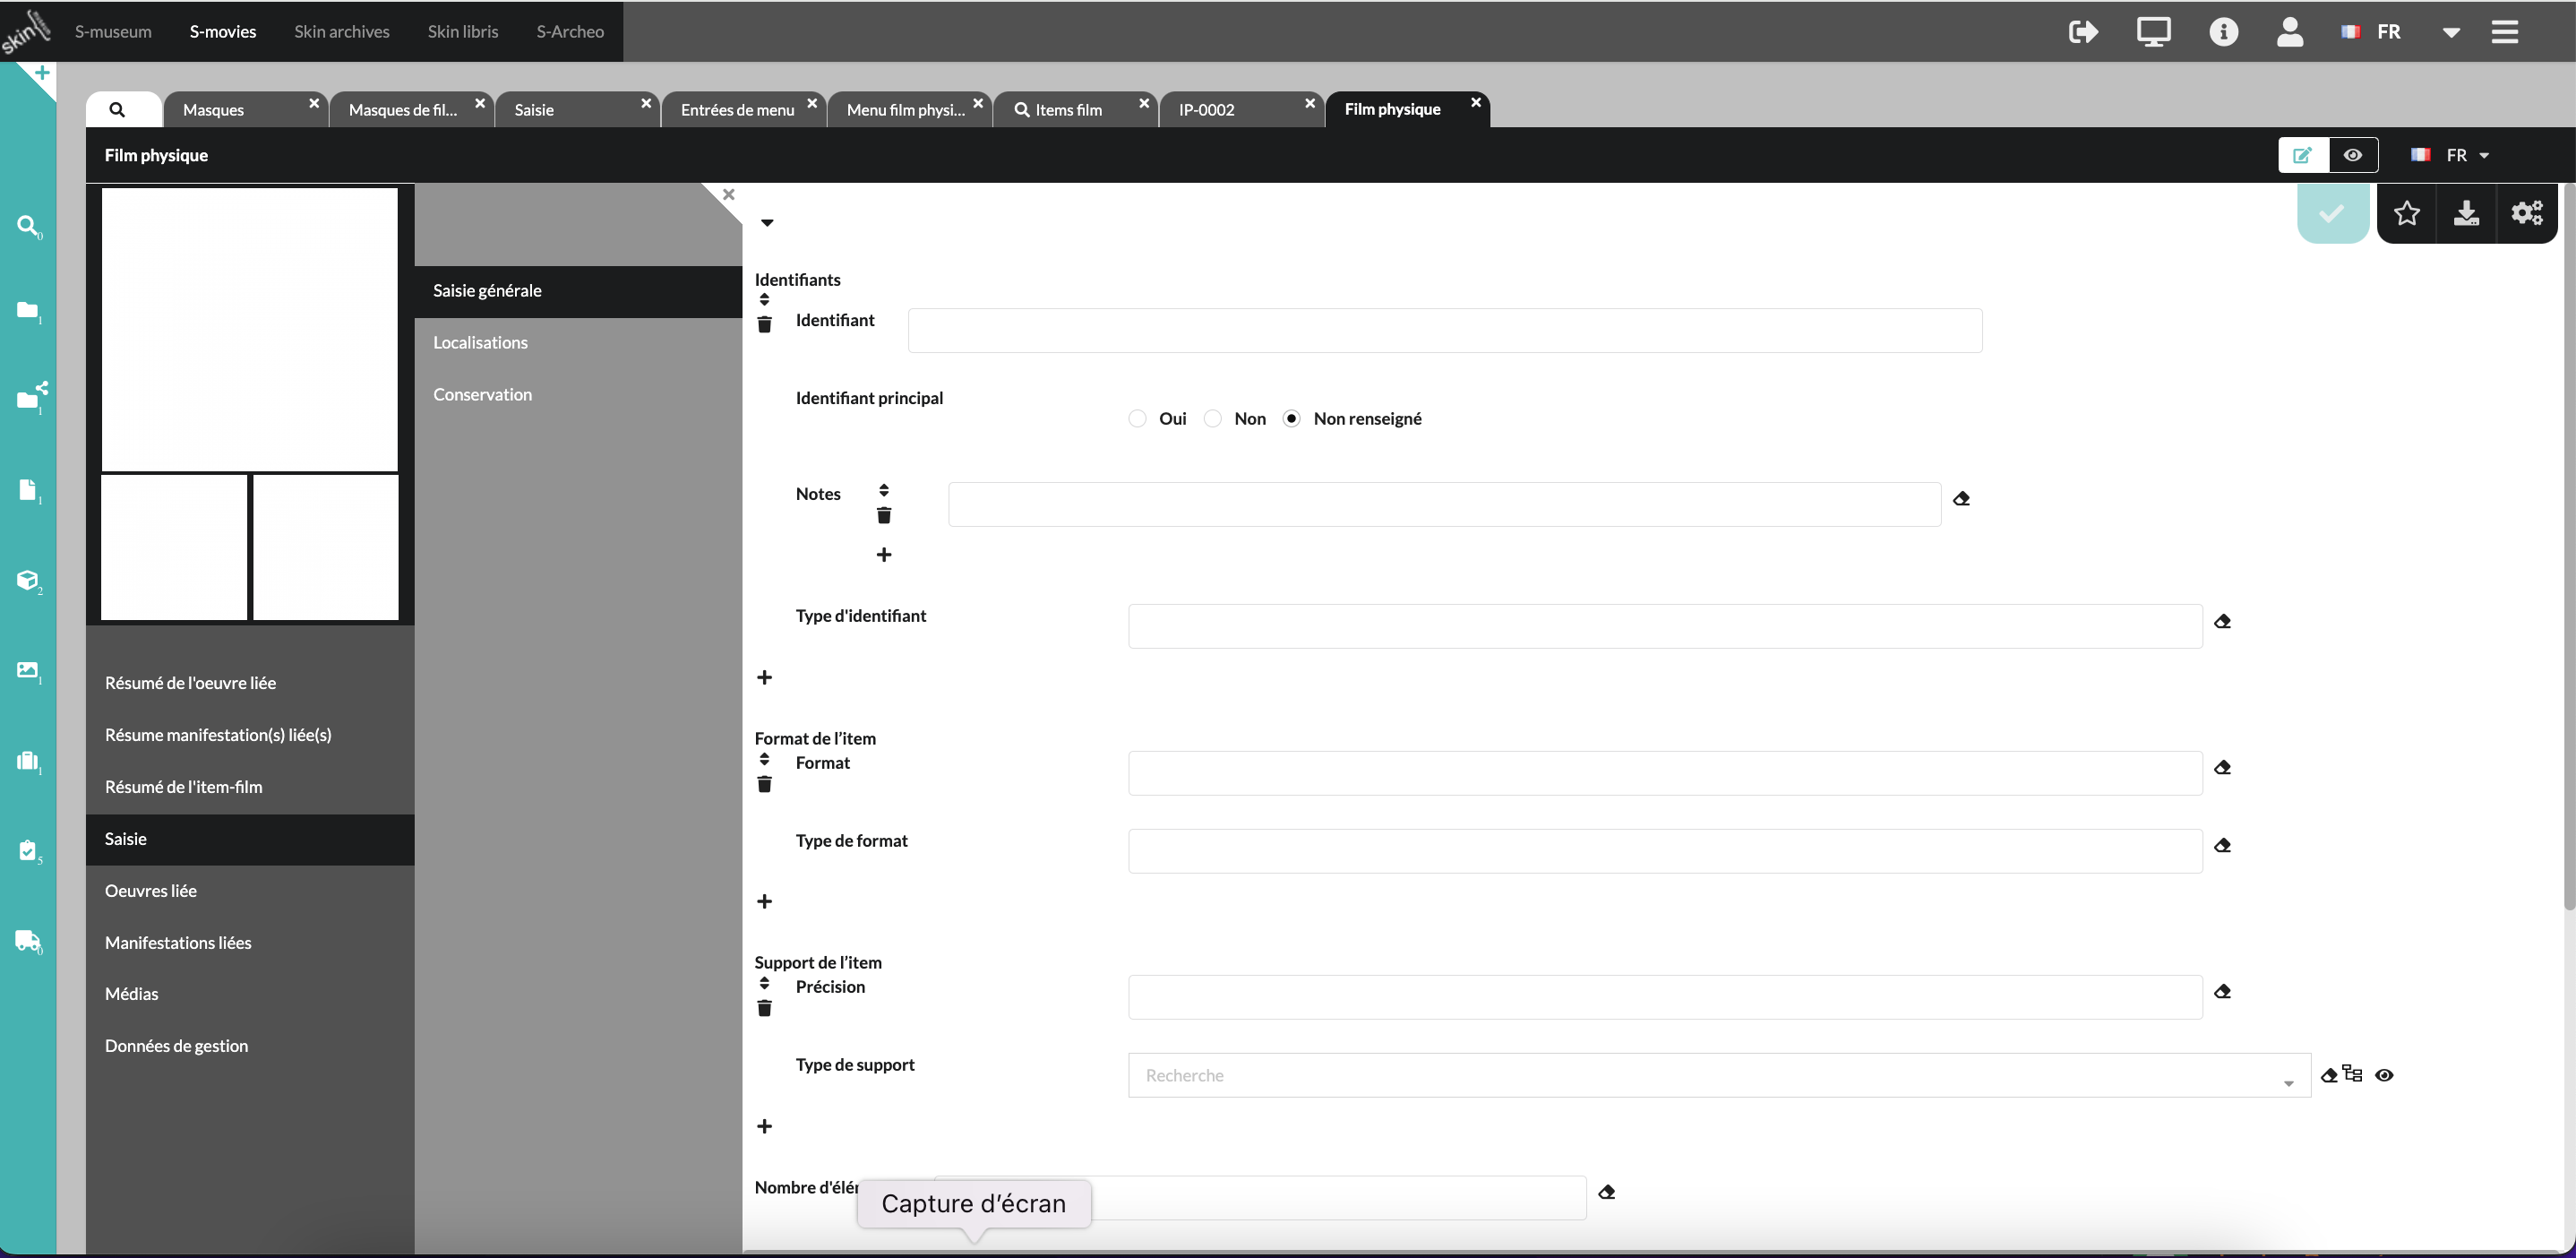
\includegraphics[width=1.0\textwidth]{images/image4.png} 
	
	\caption{Affichage du menu d'une notice de film physique à la saisie} 
	
	\label{figAffichageMenu} 
	
\end{figure}


Ce système d’organisation des masques de saisie au sein de menus permet également d’effectuer des liens avec d’autres types de notices et donc d’autres entités du FRBR. Par exemple la capture d'écran suivante \ref{figMenuGrilles}, montre que dans un menu de film physique, les onglets Œuvre liée et Manifestations liées permettent d’obtenir une grille de recherche, au sein d’une notice de film physique, affichant l’Oeuvre liée au film et les Manifestations dont il découle. 

\begin{figure}[htbp] 
	
	\centering 
	
	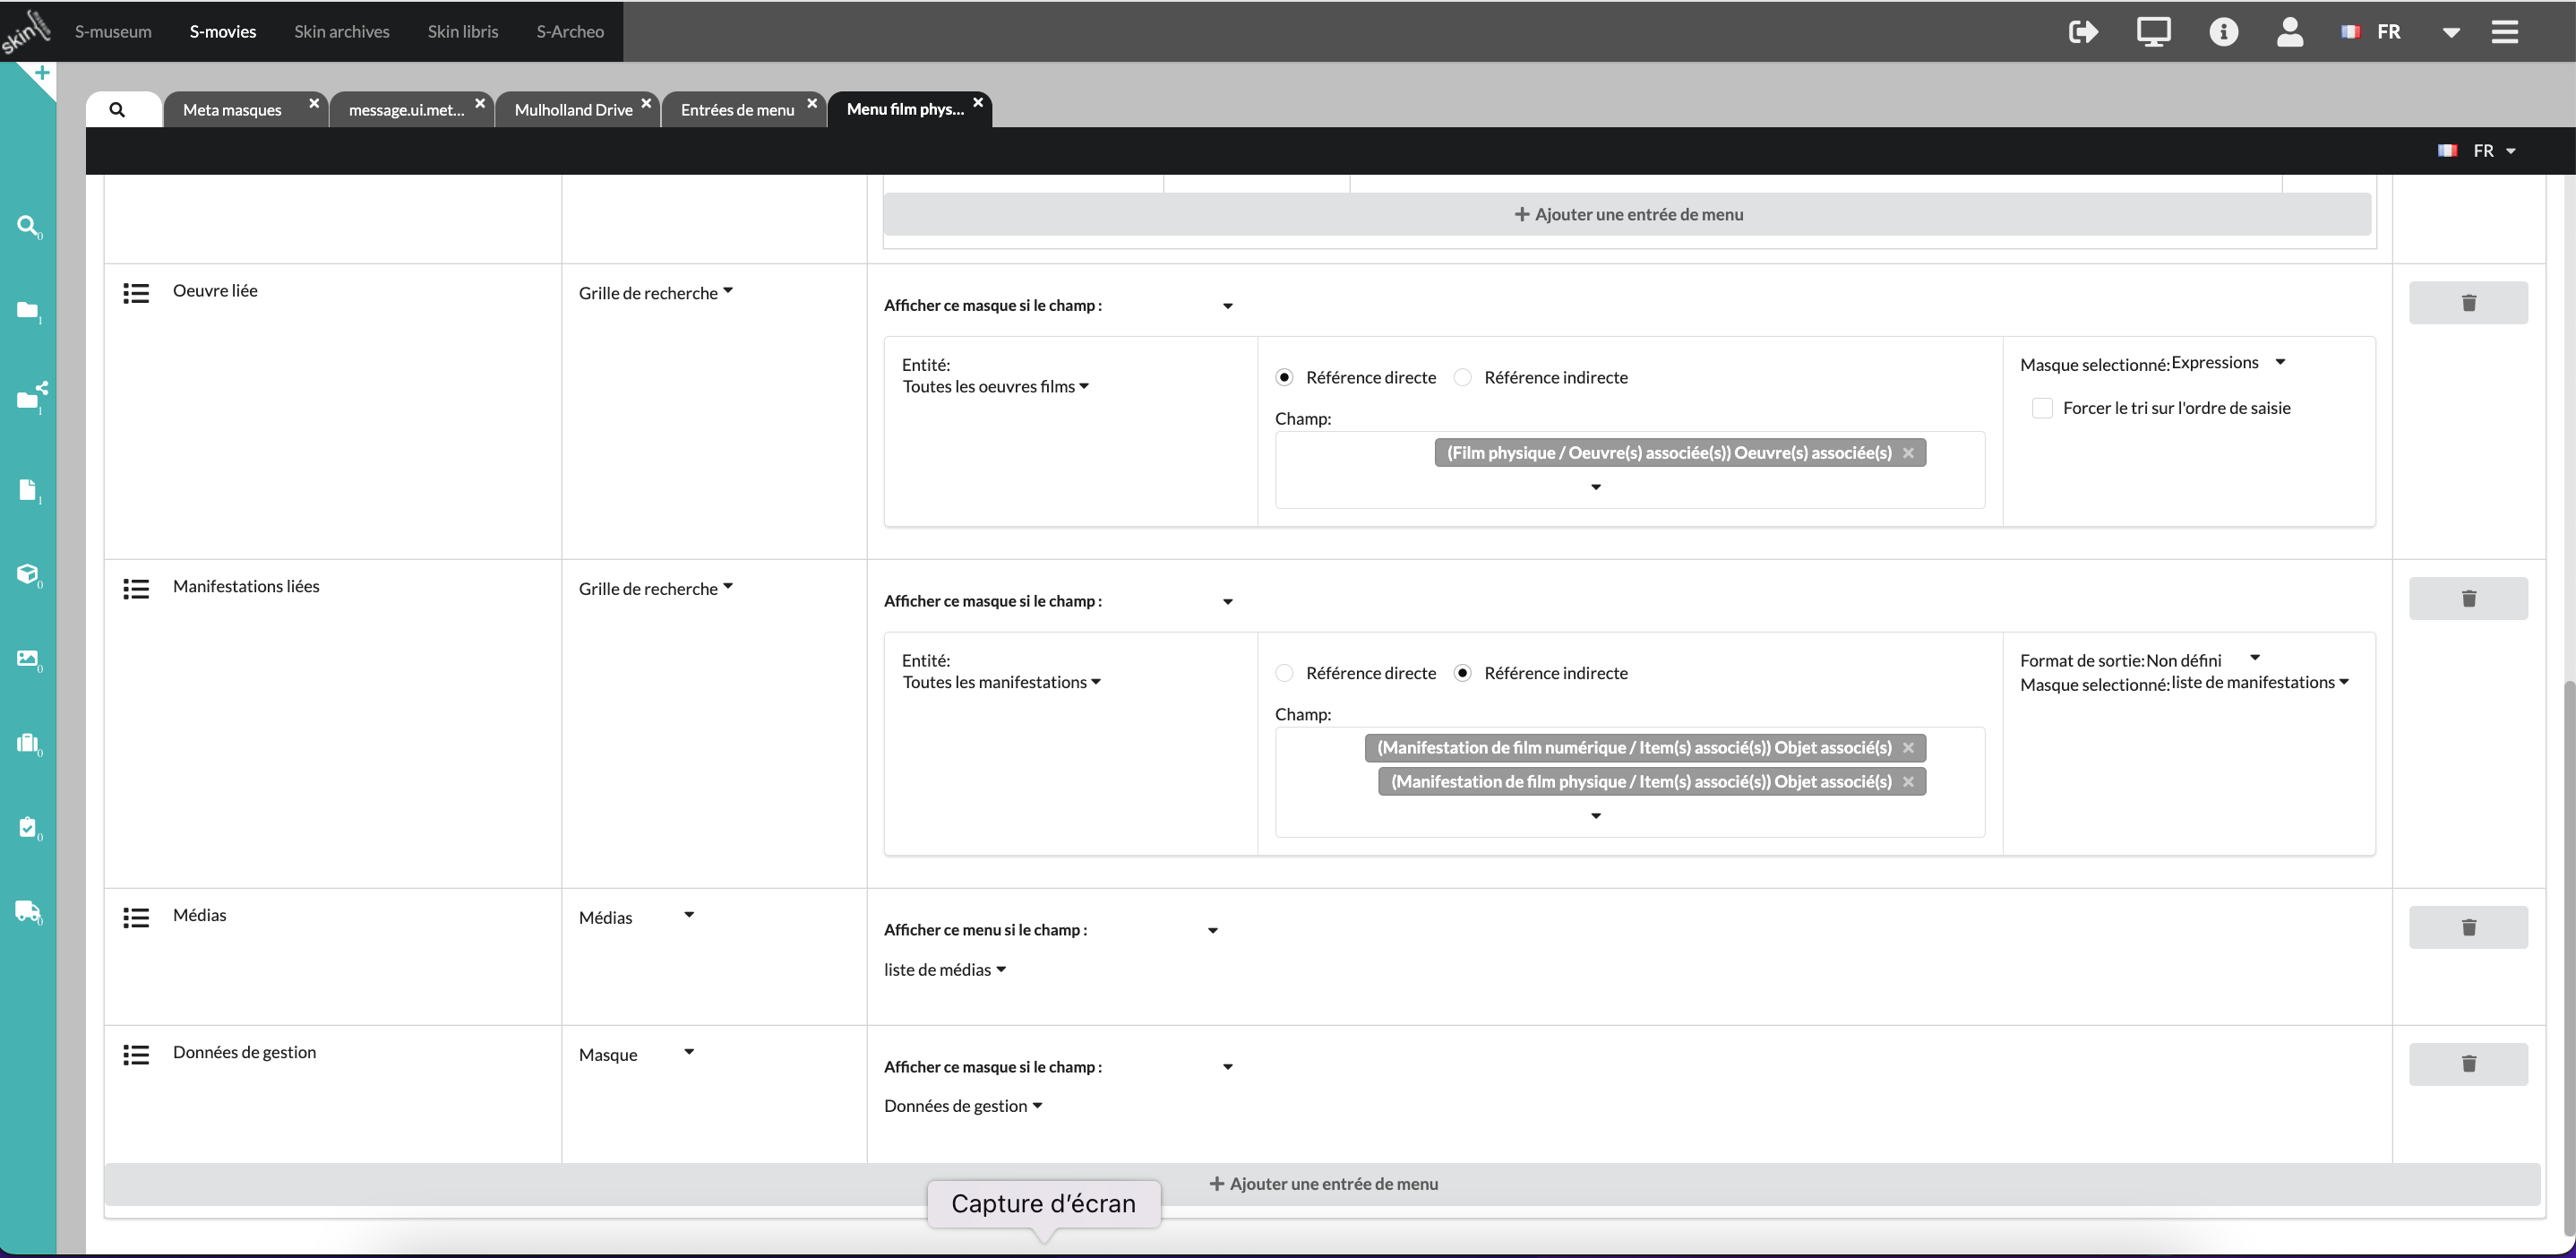
\includegraphics[width=1.0\textwidth]{images/image8.png} 
	
	\caption{Configuration de grilles de recherche pour l'affichage des éléments liés} 
	
	\label{figMenuGrilles} 
	
\end{figure}

L’affichage pour l’utilisateur au sein de la notice de film physique est le suivant, avec d’une part, l’Œuvre liée(\ref{figOeuvresLiées}, et d’autre part, les Manifestations liées \ref{figManifsLiées}: 

\begin{figure}[htbp] 
	
	\centering 
	
	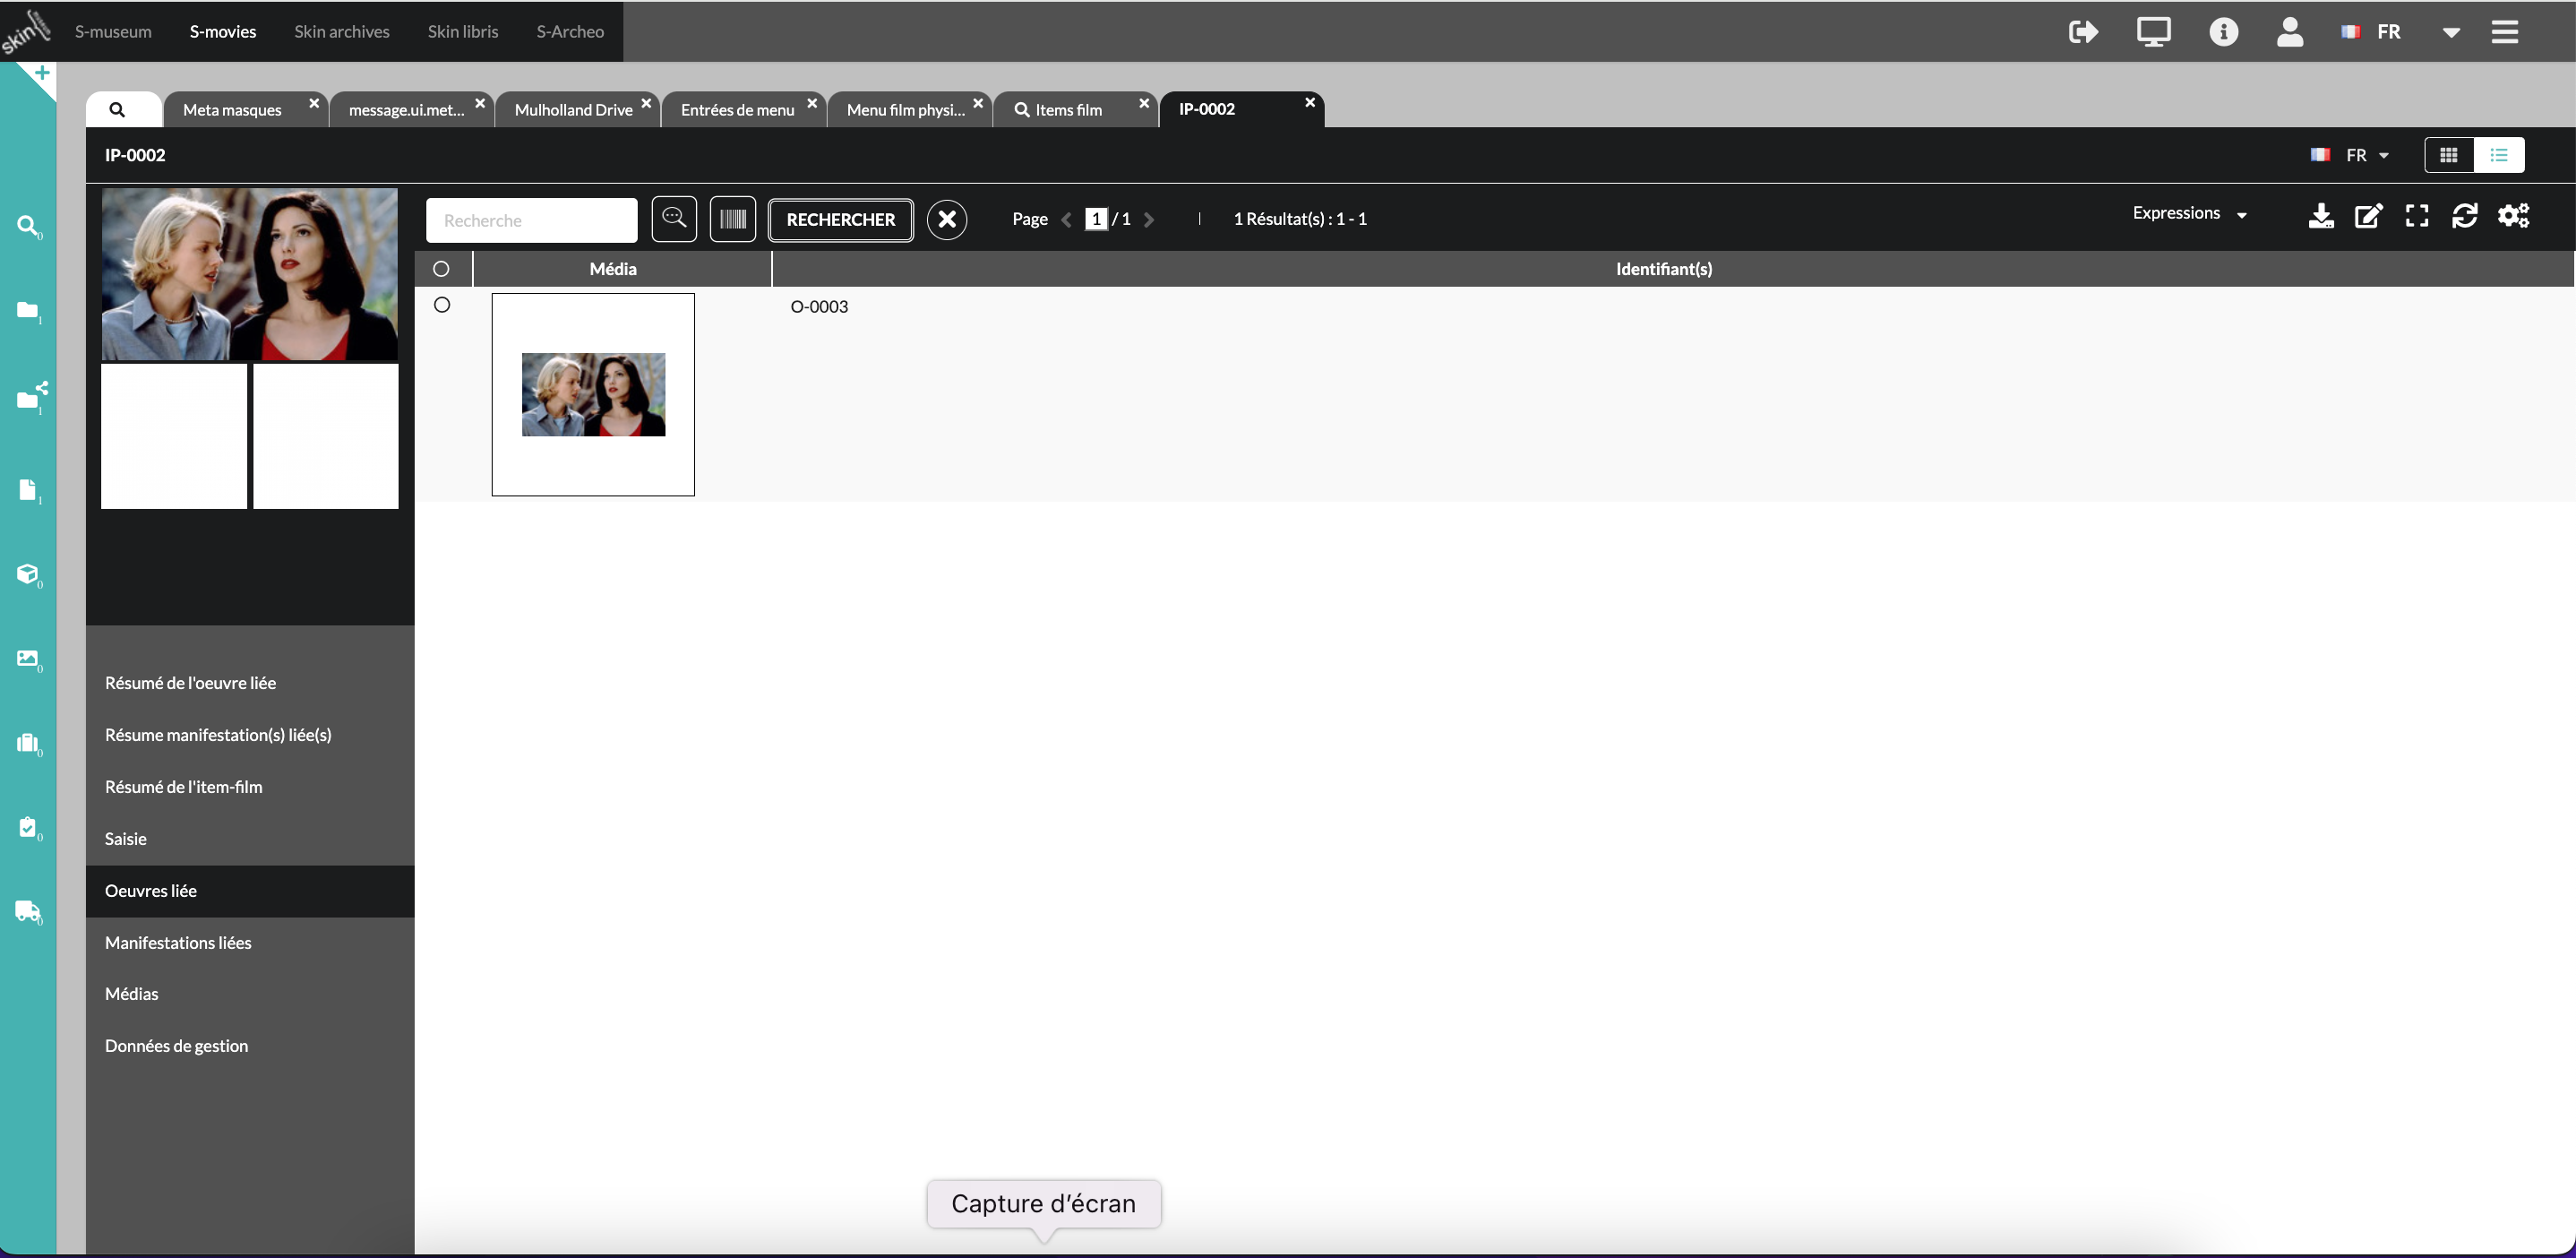
\includegraphics[width=1.0\textwidth]{images/image9.png} 
	
	\caption{Affichage des Oeuvres liées dans une notice d'item} 
	
	\label{figOeuvresLiées} 
	
\end{figure}

\begin{figure}[htbp] 
	
	\centering 
	
	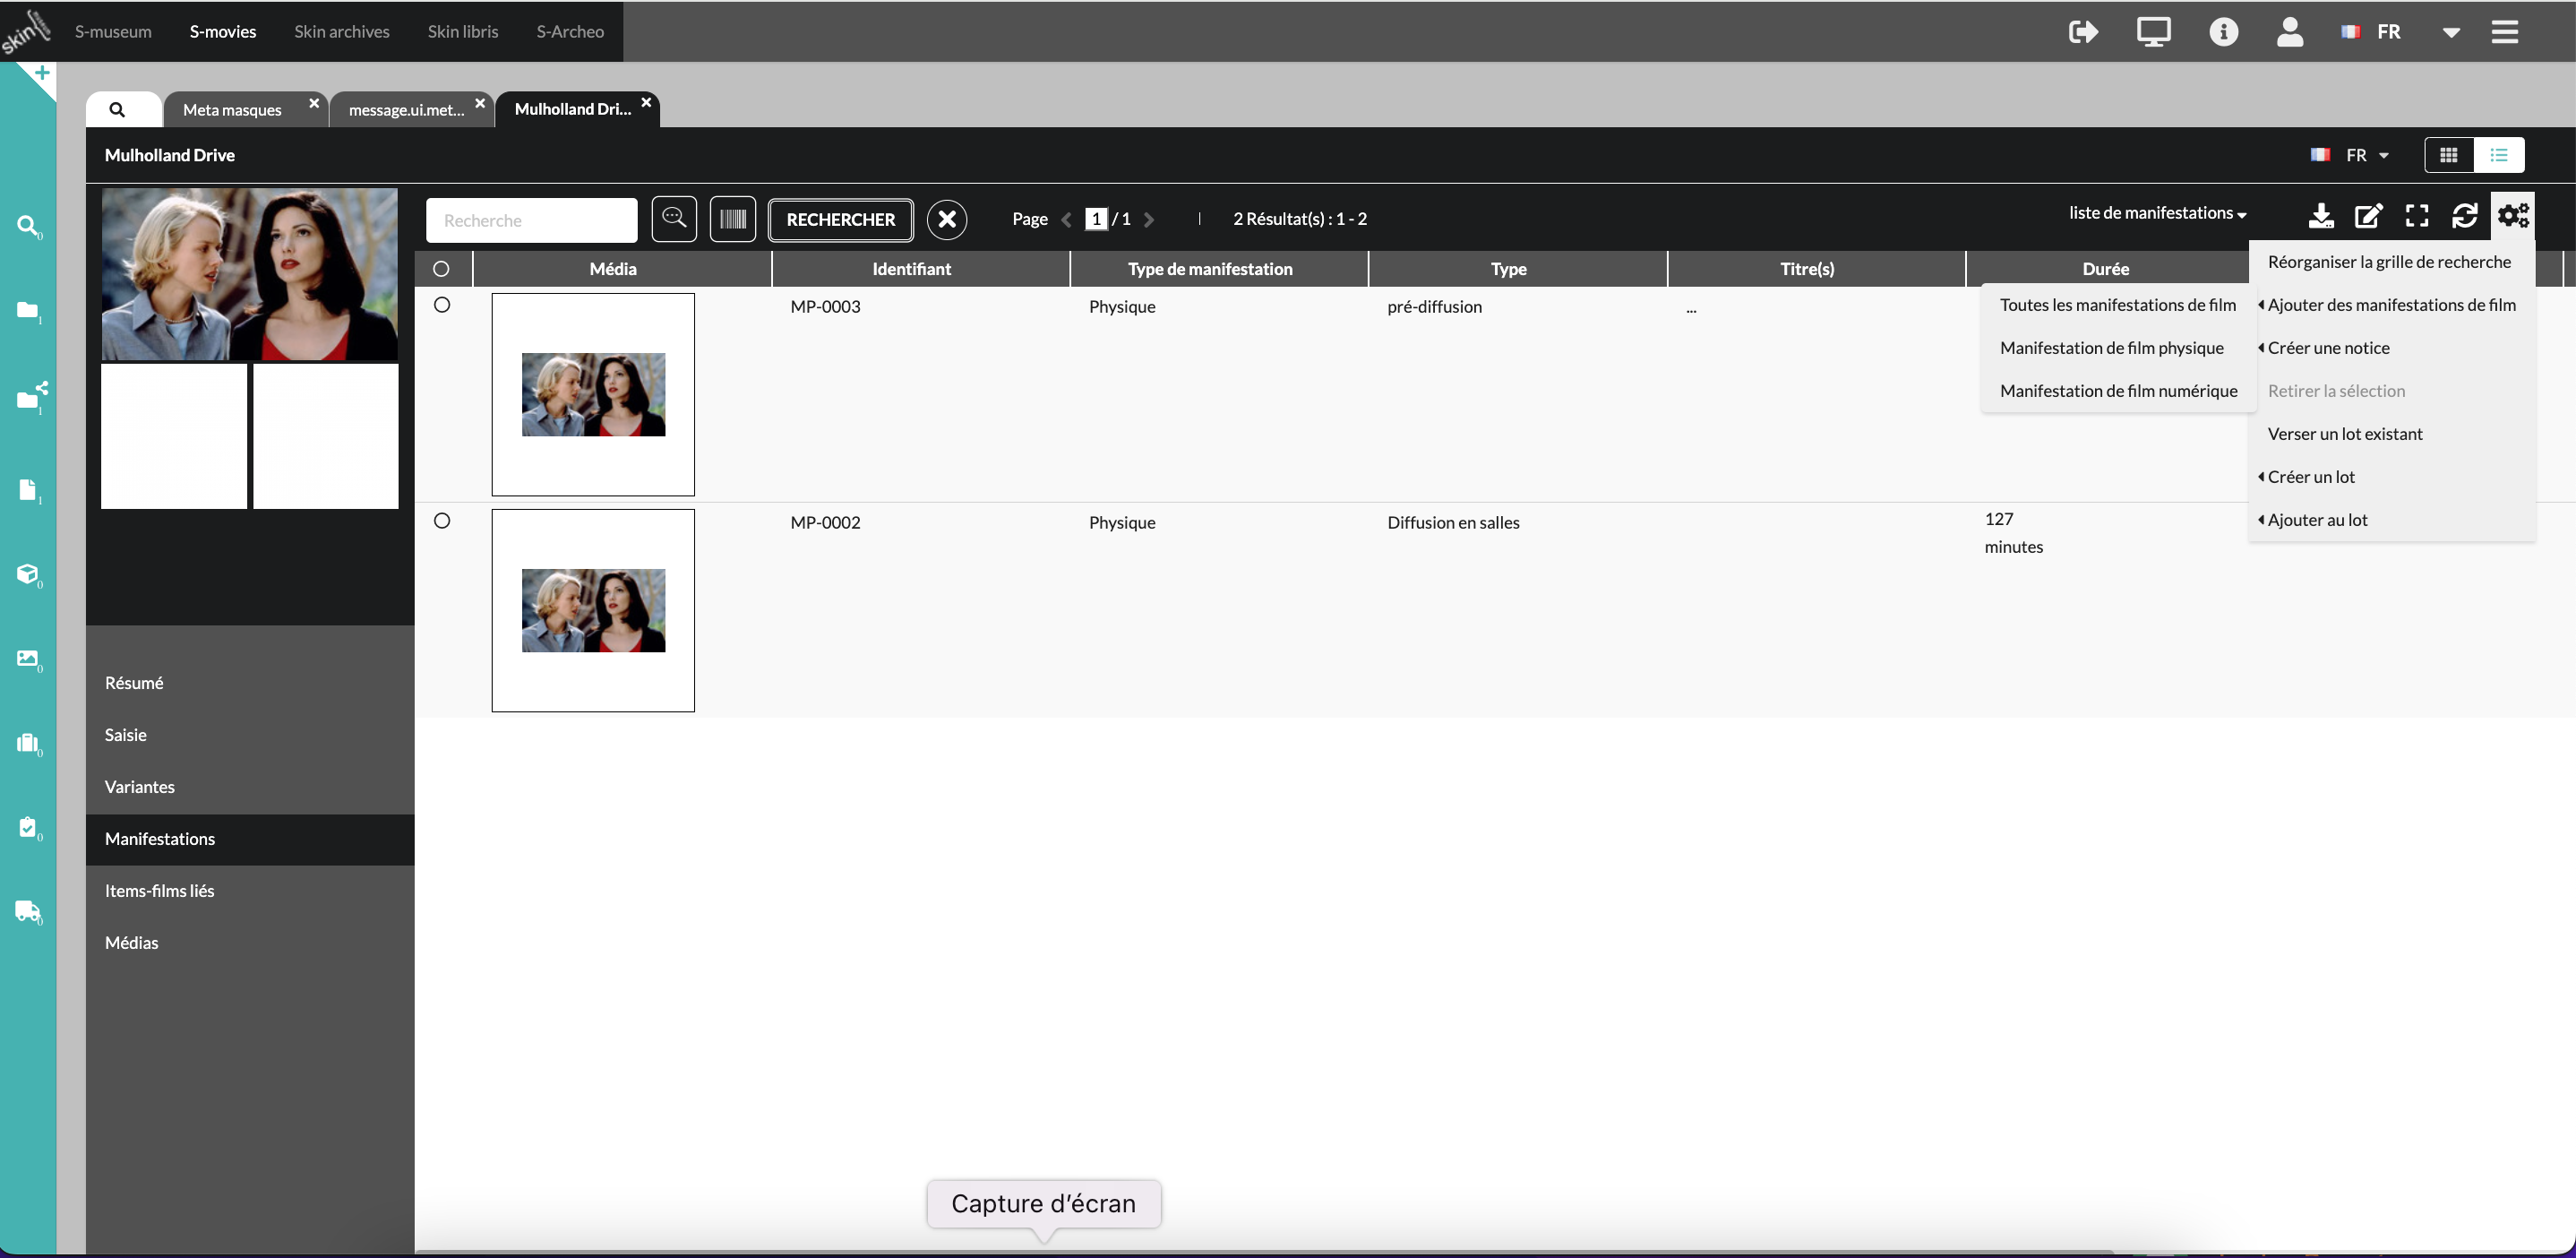
\includegraphics[width=1.0\textwidth]{images/image7.png} 
	
	\caption{Affichage des Manifestations liées dans une notice d'item} 
	
	\label{figManifsLiées} 
	
\end{figure}

Toutefois, les espaces de travail structurés sur le modèle FRBR, comme c'est le cas de S-Movies, requièrent un niveau de configuration supplémentaire, afin de concrétiser le découpage de la description en niveaux hiérarchiques. C'est le rôle des méta-masques, des formulaires de masques de saisie pouvant cibler les champs de plusieurs types de notices –et donc plusieurs niveaux du FRBR à la fois, afin d'imbriquer ces niveaux de description au sein d’une même notice. Ce système permet à l'utilisateur de saisir implicitement des éléments de description sur plusieurs niveaux du FRBR en une seule notice, permettant de surcroit au système de produire un héritage des champs d’un niveau à l’autre du FRBR.  

Concrètement, dans S-Movies, la notice d'Œuvre/Expression pointe sur les champs de l'Œuvre et de l'Expression, la notice de Manifestation pointe sur les champs de l'Œuvre, l'Expression et la Manifestation, la notice de l'Item pointe sur l'Œuvre, l'Expression, la Manifestation et l'Item. \textbf{(Faire un schéma explicatif) (citer le mode d'emploi interne ?)}. Ce mode de paramétrage de la description permet d’intégrer aux niveaux du FRBR inférieurs des champs hérités des niveaux supérieurs.  

\footnote{Notons que la présence du niveau Expression contredit le modèle FRBR préconisé par la FIAF, qui fusionne le niveau Expression dans celui d’Œuvre. Etant donné que Skinsoft possède d’autres espaces de travail modélisé sur le FRBR, comme c’est le cas de l’espace dédié à la gestion des collections bibliographiques, le niveau Expression existe seulement en théorie, mais inutilisé en pratique au sein de S-Movies.} 

Ici par exemple (\ref{figMetamasque}), un méta masque de saisie pour une notice de film physique, ciblé sur l’expression, le film physique, la manifestation de film physique, l’œuvre cinématographique : 

\begin{figure}[htbp] 
	
	\centering 
	
	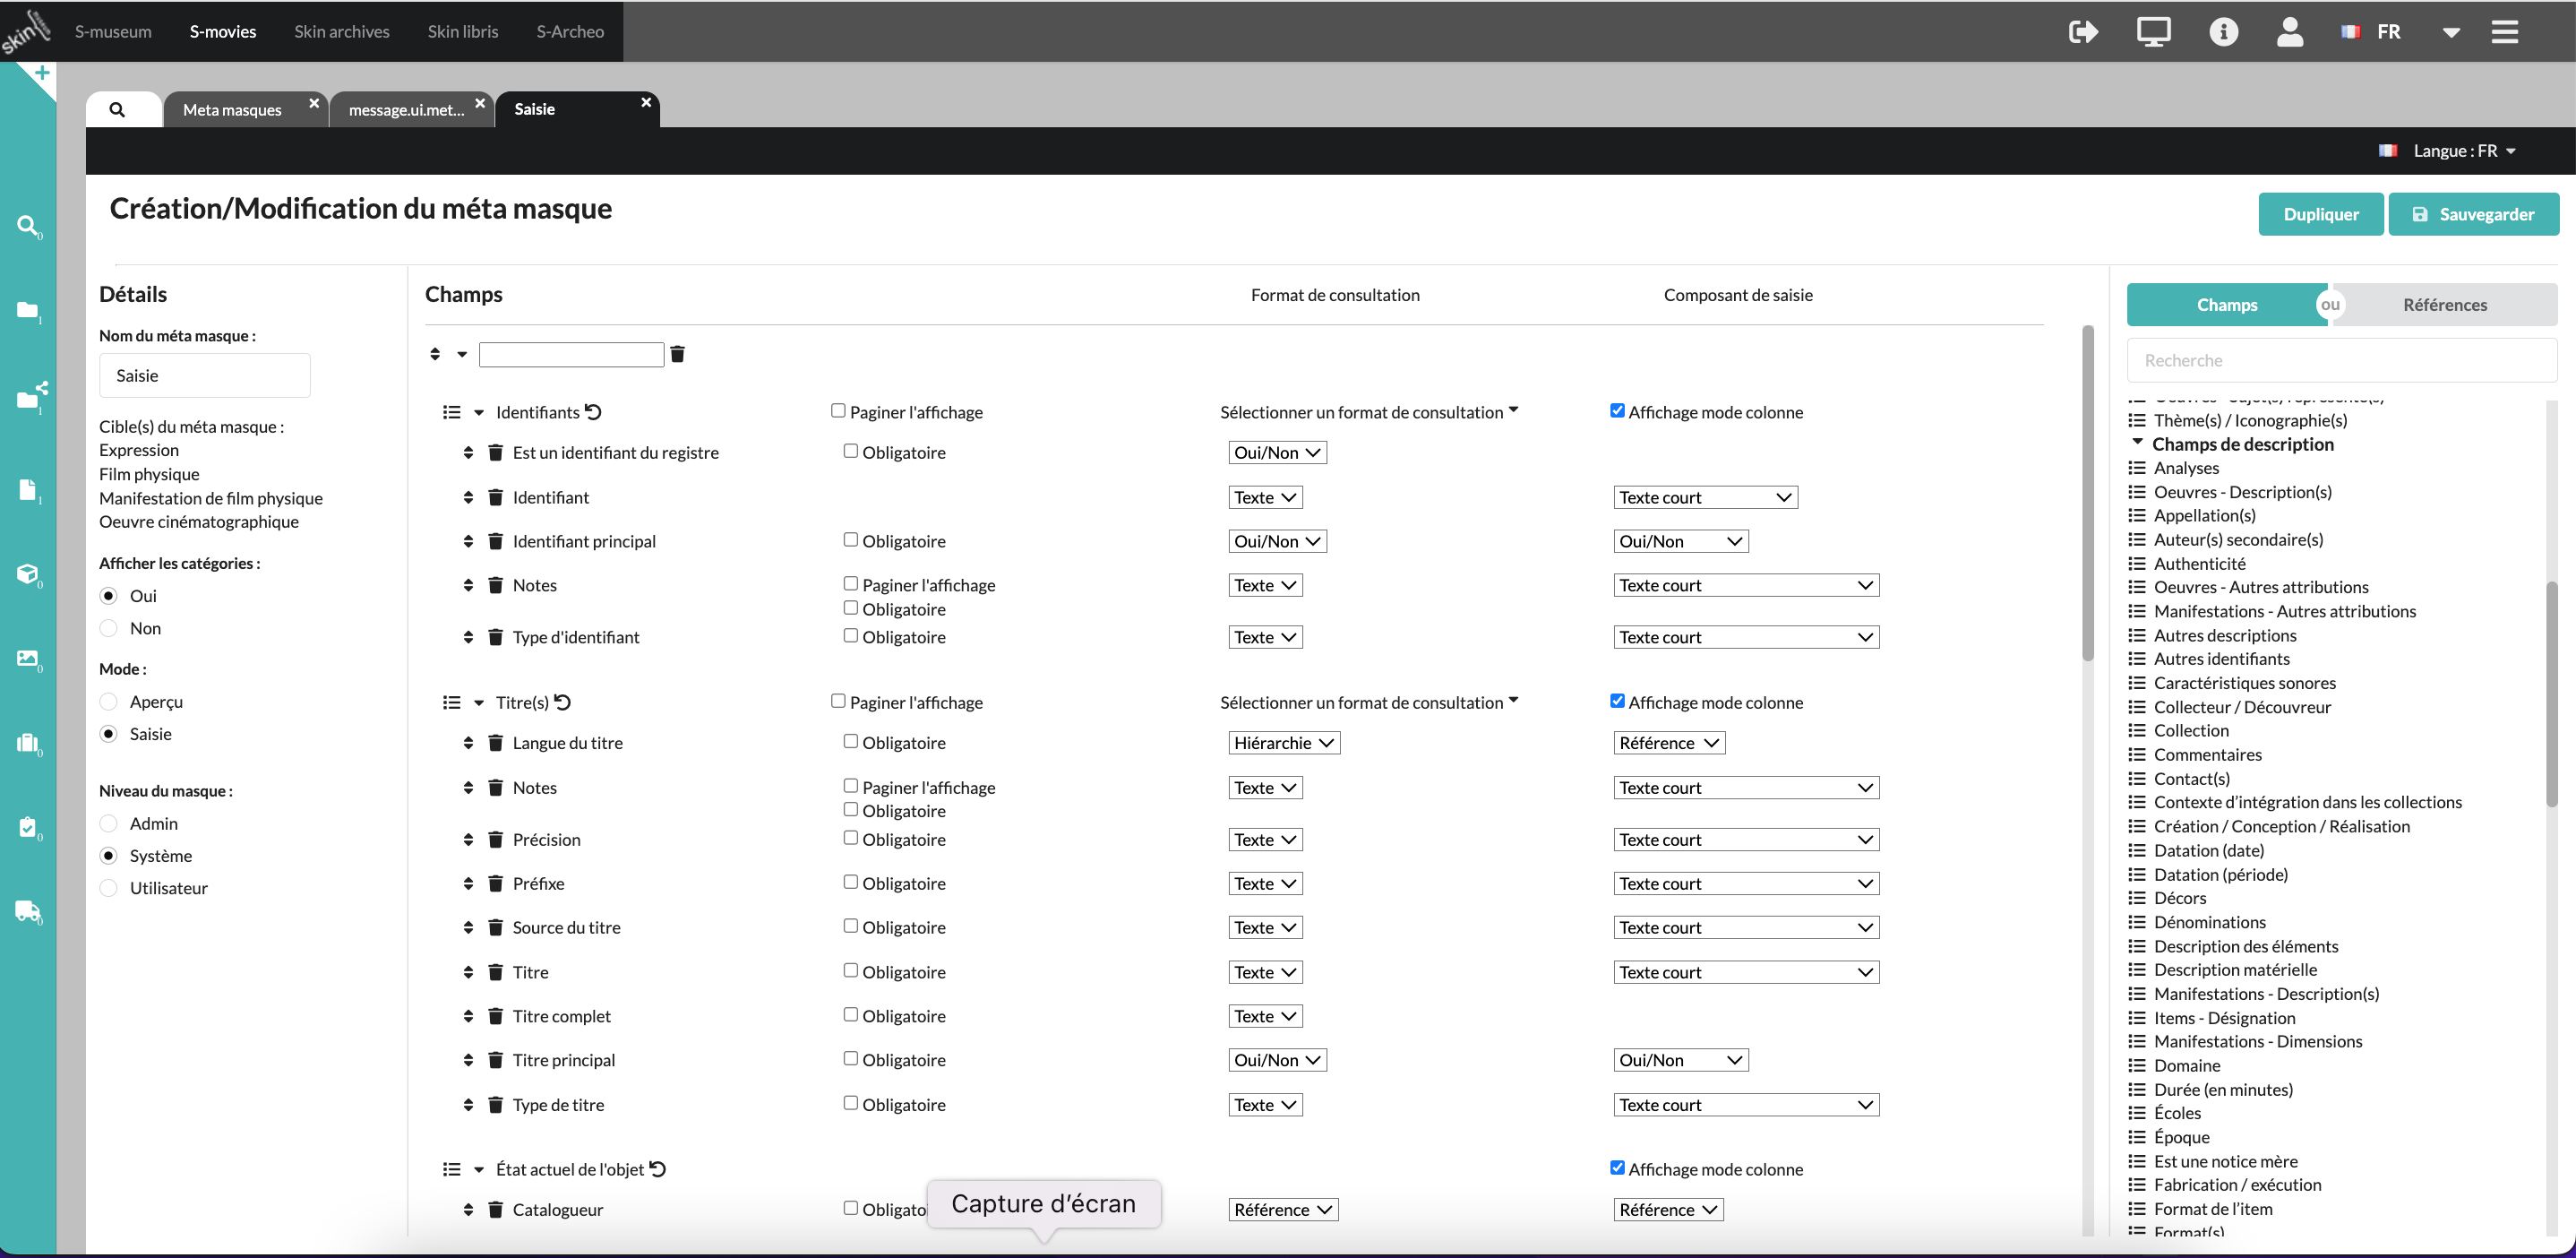
\includegraphics[width=1.0\textwidth]{images/imageb.png} 
	
	\caption{Configuration d'un méta-masque au niveau Item} 
	
	\label{figMetamasque} 
	
\end{figure}

À droite, les champs disponibles signalent à quel niveau de description ils appartiennent. Par exemple ci-dessus (\ref{figMetamasque}), le champ description appartient au niveau Œuvre, le champ dimensions appartient au niveau Manifestation.

%(: média (notice du fichier numérique, média), accessoire (modèle d'accessoire, accessoire), contenant (modèle de contenant, contenant).) 

Ces masques et méta masques créent ainsi une structure pérenne qui fait l'objet d'un paramétrage individuel qui permet d’ajuster la structure en fonction du type de collection et des usages métiers du client concerné. Ce paramétrage est défini au cours d’un travail de mapping entre les données client et la structure proposée par Skinsoft, afin de trouver un accord sur les champs qui seront utilisés pour la description des collections. L'équipe de Skinsoft organise ensuite ces champs dans des formulaires de saisie (masques et méta masques), eux-mêmes organisés pour constituer des menus de notice et des grilles de résultats de recherche. L'équipe produit également des imports de thésaurus propres aux usages de l'institution en question, afin d'assurer l'interopérabilité des données saisies. %Afin d'assurer l'interopérabilité des données, l'indexation des champs est liée à des thésaurus et des référentiels contrôlés qui ont importés au moment de la configuration de l'espace de travail pour le client. À développer  

Les fondements de l'architecture de S-Movies, doublement adaptée d’une part aux collections cinématographiques et d’autre part aux pratiques métiers spécifiques à chaque institution, constitue la condition de la qualité des données et de l’expérience utilisateur. L'enjeu de l'espace de travail est d'offrir une interface qui permette à l'utilisateur de décrire les collections en plusieurs niveaux sans difficulté et de pouvoir circuler entre ces niveaux et les liens qu’ils entretiennent. Cette circulation est notamment permise par les grilles de recherche que nous avons évoquées dont le paramétrage permet d’afficher les entités liées pour chaque notice. De plus, les différents outils de recherche permettent de circuler au sein des éléments de description indexés. (À développer ?) 

Toutefois, malgré la haute configurabilité de l’interface, l’hétérogénéité des corpus audiovisuels gérés d’une institution à l’autre complexifie le travail de mapping qui doit être effectué. En effet, la modélisation FRBR préconisée par la FIAF est un cadre qu’il s’agit d’ajuster aux pratiques spécifiques de gestion des collections, elles-mêmes adaptées au type de corpus géré. L’ajustement à des corpus audiovisuels spécifiques complexifie potentiellement la fluidité de la navigation entre les liens des différentes entités du FRBR au sein de l’interface.   

%Présentation espace S-Movies : aperçu des fonctionnalités communes et spécifiques (à placer en annexe ?): ces fonctionnalités sont chacune rattachées à un ou plusieurs niveaux du FRBR 

%- gestion des entrées : création d'un objet de collection via l'import de son média 

%- gestion des médias : associer un nouveau média à une notice de film ou un média existant 

%définir des vignettes sur les notices de films à l'aide des médias importés  

%- documents associés  

%- table collections/thématiques : regroupement des collections par thématiques : décrit le contexte de la collection, de l'assemblage des films, et présentent les items présents dans cette collection 

%- projets et mouvements : intervention, conservation, acquisitions, entrées, expositions, prêts, diffusion/programmation 

%fonctionnalités communes : gestion des contrats, évènements, interventions, expositions 

%Lien de la FIAF à S-Movies : mise en application du manuel de la FIAF, remodélisation, adaptable selon les corpus. tension public/privé 



%à bouger dans la première sous partie 

%S- Movies s'appuie sur deux normes descriptives audiovisuelles européennes : la norme EN 15744, qui définit le contenu obligatoire de description pour l'identification d'un film, ainsi que la norme EN 15907 qui découle du manuel de la FIAF et décrit une structure en couches et niveaux de données. Ces normes définissent les métadonnées essentielles pour faciliter l'échange de données et l'identification des films. \footcite{zotero-item-646} 



%Au niveau de la description des archives, il s'appuie sur la norme RDA pour la description et l'accès aux ressources. \footcite{zotero-item-646} 

%mentionner les données techniques ? : type de serveur, type de base de données 




\subsubsection{L'inscription des corpus de données dans la remodélisation du FRBR} 

En effet, la nature du corpus audiovisuel complexifie le paramétrage puisqu'elle conditionne la capacité des données à s'adapter et s'intégrer au sein du modèle FRBR. Le modèle FRBR fait partie d'une structure fixe de l'espace de travail, avec cette séparation en trois tables de saisie (Œuvres, Manifestations, Films), dont le paramétrage peut toutefois amoindrir la rigidité. Afin d'analyser la mesure dans laquelle les corpus s'intègrent au sein du modèle FRBR, nous analyserons dans cette sous partie deux corpus de données différents gérés au sein de l’application Skinsoft. \footnote{Notons que pour des raisons de confidentialité, nous décrirons les corpus de ces institutions sans les nommer de manière explicite.}.  

Premièrement, analysons l'intégration d'un corpus de cinéma dit "classique", au sein de l'espace de travail S-Movies. Cette collection est gérée par une institution qui préserve essentiellement des films de fiction issus d'une production commerciale "grand public" depuis les débuts du cinéma jusqu'à nos jours. Cette collection est composée d’œuvres cinématographiques à proprement parlé, dont la description prend tout son sens au sein d’une modélisation selon le FRBR. La production cinématographique étant une production industrielle, les films qui en sont issus s'adaptent particulièrement bien à un modèle de données par niveaux, ces différents niveaux correspondant aux étapes de production. Ces films, après leur création, ont donc été produits et distribué à une échelle plus ou moins large. Ainsi, dans ce cas précis, le modèle FRBR est plutôt bien adapté. La réalisation du film par le montage et le tournage est décrite au niveau Œuvre, ses versions sont décrites au niveau variante, son édition et sa distribution sont décrites au niveau Manifestation, et l'exemplaire individuel du film, conservé par l'institution est décrit au niveau Item. De fait, le paramétrage décrit dans le chapitre précédent peut être réalisé sans trop de complexité au sein du cadre modélisé par le FRBR de la FIAF. (Développer + ?) 

Deuxièmement, analysons l'implémentation d'un corpus plus spécifique, celui d'une collection de \textit{rushes} documentaires muets et non montés, tournées des années 1910 à 1920. Les \textit{rushes} en termes cinématographiques correspondent à des épreuves de tournages non montées\footcite{universalis.} Ces \textit{rushes} bruts, ont été tourné dans une optique de documentation sur différents sujets, et ne sont pas destinés à une diffusion auprès du grand public. 

Dans ce cas, l'absence de montage et de distribution commerciale rend difficile l'adaptation du corpus à la modélisation prévue par la FIAF, qui structure S-Movies. Si le contexte de création du tournage peut être décrit au niveau Œuvre, les niveaux de description inférieurs sont inadaptés. En effet, en l'absence de montage, la Variante n'existe pas puisque chaque \textit{rushe} correspond à une matière brute et unique. Ainsi, l'absence de différentes versions d'une même œuvre invalide l'entité de Variante.  

De la même façon, le niveau Manifestation perd de sa pertinence descriptive puisque ces \textit{rushes} ne sont ni produits ni distribué officiellement auprès d'un public. L'inscription de l'œuvre sur un support s'effectue ici de manière unique, et en un seul et même exemplaire. Les caractéristiques matérielles pourraient donc être décrites directement au niveau de l'item.  Ainsi, d'un modèle à quatre niveaux, il ne reste, dans ce cas précis, plus que deux niveaux de descriptions exploitables : l’Œuvre et l’Item. Toutefois, notamment pour des raisons de conservation, une œuvre peut être copiée sur différents supports, physiques ou numériques. En effet, l'institution peut être amenée à produire des copies d’une œuvre sur des supports plus stables à des fins de préservation ou de diffusion en ligne, par exemple. Ces différentes matérialisations, bien qu'elles ne soient pas issues d'un processus commercial de distribution, peuvent être décrites comme des Manifestations. Telle que définie par le manuel de la FIAF, une manifestation induit en effet, "tous les médias analogiques, numériques et en ligne associés à une matérialisation particulière d'une Œuvre/Variante." \footcite{zotero-item-646}. Sa description peut alors être justifiée par des objectifs de conservation : copie, numérisation, restauration. Selon le FIAF, la description d'une Manifestation inclut les attributs suivants, -ici sélectionnés selon leur niveau de pertinence pour un tel corpus : type de manifestation, format (incluant les champs suivants : type de support, caractéristiques sonores, caractéristiques de couleur), notes.  

Or, si théoriquement le niveau Manifestation peut être décrit, en pratique dans le cas de la description de ce corpus produite par l’institution, il ne l’est pas. Est-ce que le modèle de description utilisé en pratique correspond au modèle à deux niveaux présentés brièvement par la FIAF ?  

Si au sein d'une notice d'œuvre, les champs suivants sont décrits : identification, titre, créateur, description (sujet de la prise de vue), mots clés, films associés, manifestations associées, matériel non-film associé, archives associées, bibliographie, médias, données de gestion ; la table Manifestations, en revanche, contient un nombre conséquent de notices vides. En effet, l'application Skinsoft crée automatiquement une notice de manifestation liée lorsque l'utilisateur crée une notice d'item. Dans ce cas, l’entité Manifestation devient une condition structurelle afin de maintenir la cohérence du modèle, mais perd son sens au sein d’un contexte d'indexation concret. La table des items, quant à elle, est répartie en trois catégories d'objets : bobines, cassettes ---qui constituent les films physiques--- et films numériques. Lorsqu'un même film physique est présent en plusieurs exemplaires dans la collection, les notices sont distinguées par la mention "bobine originale" et "reproduction". Les notices de films physiques contiennent une description matérielle sur le support et la condition de ce support. Elles mentionnent également les collections liées vers d'autres Items et Œuvres, vers des médias et des documents. La manifestation référente est tout de même mentionnée mais il s'agit, nous l'avons évoqué, d'une notice factice. Enfin, les films numériques décrivent le support original depuis lequel la numérisation a été effectuée, les raisons de la numérisation ---par exemple, copie de sauvegarde---, et l'item physique qui a fait l'objet de cette numérisation.  

Par ailleurs, un élément précis a retenu notre attention dans le cadre de notre étude. En effet, la présence de \textit{time-codes} ---marqueurs temporels dans des notices de films numériques, traduisant l'inscription de la copie numérisée dans une œuvre plus large. En effet, certaines Œuvres-rushes, dont les modalités matérielles sont décrites dans une notice de film physique, ont été divisées en extraits puis numérisées. Étant donné que les Œuvres conservées sont des rushes non montés, cette division en extraits a pour but de réaliser une forme de montage et de rendre ces films intelligibles via une diffusion en ligne. Ainsi, la plupart des films numériques gérés au sein de S-Movies sont issus de ce découpage depuis les rushes originaux. Les repères temporels expriment le rattachement précis de l'item numérique au sein d'un item physique.  

Ainsi, la modélisation de données adaptées à ce corpus audiovisuel précis s'apparente à un modèle hiérarchique à deux niveaux, celui d'une Œuvre matérialisée dans une Manifestation/Item, fusionnés en une seule entité. Cette hiérarchie à deux niveaux est brièvement décrite dans le catalogue de la FIAF en tant qu'exemple, mais ses modalités ne sont pas détaillées. (À développer?) 

\begin{figure}[htbp] 
	
	\centering 
	
	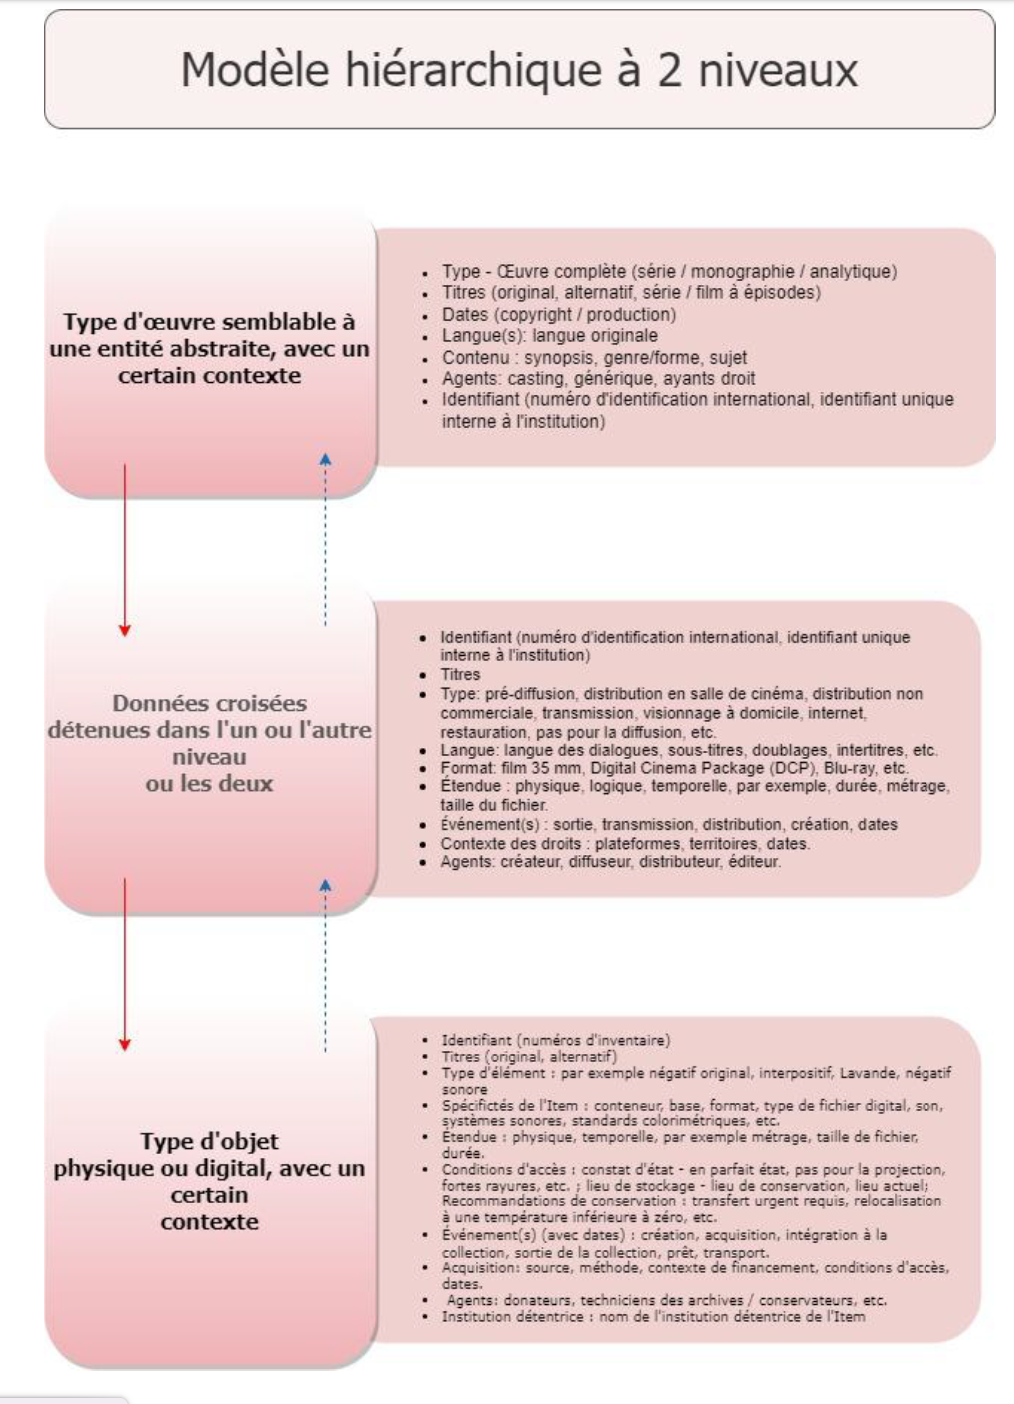
\includegraphics[width=1.0\textwidth]{images/imagec.png} 
	
	\caption{Modèle hiérarchique à deux niveaux schématisé par le manuel de la FIAF} 
	
	\label{figModele2Niveaux} 
	
\end{figure}

Développer davantage le schéma de données que ça produit dans l’appli client ? Avec un schéma ? À partir des captures d’écran suivantes : schématiser les liens complexes entre éléments pour le corpus en question  

Par exemple : Une notice Œuvre est liée à un item numérique, lui- même lié à un ou plusieurs films physiques : cassette, bobine, avec le time code mentionné pour traduire la place de l’extrait/film numérique au sein de ces supports physiques.  

Les films physiques : contiennent la liste des films numériques qu’ils ont pour extrait + les différentes reproductions du film physiques sur d’autres supports physiques : plusieurs bobines, plusieurs cassettes (à des fins de conservation)  

Si l'espace de travail S-Movies parvient à maintenir le modèle du FRBR en trois niveaux principaux pour les corpus audiovisuels standards, la description de corpus plus spécifiques éclipse notamment le niveau Manifestation pour ne conserver qu'une hiérarchie à deux niveaux. L’analyse de l’inscription d’un corpus donné au sein de la modélisation de données proposée par S-Movies soulève des interrogations sur la fluidité de la navigation de l’utilisateur au sein de l’interface.  En effet, le caractère brut du corpus observé nécessite une description fine du contenu afin de restituer une intelligibilité, d’habitude produite par le montage, qui doit être prévue par une saisie ergonomique au sein de l’interface. Afin d’adapter l’espace de travail à des corpus aussi spécifiques, l’éditeur Skinsoft engage notamment une démarche de refonte de S-Movies, dont l’objectif est de repenser d’une part l’interface fondée sur le FRBR, et d’autre part d’intégrer des fonctionnalités innovantes d’indexation automatique afin d’assister l’utilisateur dans la description des collections. C’est dans ce contexte d’innovation technique que s’inscrit notre stage, au cours duquel nous avons étudié l’usage de S-Movies afin d'en améliorer l’expérience utilisateur, et ainsi préparer l’implémentation de fonctionnalités automatiques pour la description des collections audiovisuelles.  

\subsubsection{Vers une refonte de S-Movies} 

Si le cadre posé par la modélisation FRBR s’avère limité pour des collections spécifiques telles que celles que nous avons analysé, le modèle induit des difficultés plus globales au niveau de l’interface et de la navigation utilisateur. Le FRBR est fondé sur des besoins utilisateurs dont l’objectif serait “d’identifier, sélectionner et acquérir” efficacement l’ensemble des éléments décrits et répartis entre différents nie=veaux hiérarchiues \footcite{zotero-item-646}. Ces besoins semblent respectés au sein de l’interface S-Movies, via la navigation permise entre les entités et les outils de recherche disponibles. Toutefois, une double complexité subsiste dans l’implémentation de la modélisation FRBR au sein d’une interface. D’une part, il reste complexe de mettre en place une interface intuitive permettant à l’utilisateur de connaître immédiatement le rôle descriptif de telle entité du FRBR et sa place au sein de la hiérarchie du modèle. D’autre part, la visualisation des liens entre les entités du FRBR reste limitée, puisqu’elle supposerait des développements supplémentaires innovants tels que la visualisation en graphe, par exemple.  

Parmi les complexités d’interface révélés par l'expérience utilisateur, certains éléments semblent anodins. Par exemple, l’affichage d’une hiérarchie inversée du FRBR dans le menu de l’application, pouvant nuire à l’intuitivité du rôle de chaque entité pour la description des collections. En effet, au sein du menu, les tables sont présentées de telle manière à ce que le plus bas niveau du FRBR (l'item) apparaisse en haut, suivi de la manifestation et du plus haut niveau (l'œuvre). Cet affichage visuel descendant peut induire en erreur l'utilisateur sur la navigation hiérarchique à employer au sein du modèle. De plus, au sein de S-Movies le plus bas niveau de la hiérarchie (l’Item) est désigné par la notion de “Film”. Or, dans un contexte cinématographique, le film peut communément désigner à la fois une œuvre et un item individuel. La notion de film n'évoque pas le caractère unique et individuel de l'exemplaire tel qu'il est défini par le manuel de la FIAF. Une autre confusion terminologique potentielle peut être créée par la présence de la notion d'Expression, alors même que ce niveau, issu du modèle FRBR bibliographique, est fusionné dans celui d'œuvre.  

La visualisation des liens entre les entités descriptives au sein de l’interface est également motrice d’améliorations au sein de l’espace de travail. L'interface actuelle permet, après configuration, de visualiser les liens d’une notice avec d’autres notices issues de niveaux différents du FRBR. Or, il serait pertinent pour l’utilisateur d’avoir la possibilité de visualiser les liens entre entités à un niveau plus large, et de manière graphique. Par exemple, il serait pertinent de pouvoir visualiser, au niveau d’une notice Œuvre, l'ensemble des manifestations dans lesquelles elle est matérialisée, ainsi que tous les exemplaires issus de ses manifestations respectives et conservés par l’institution. Cette visualisation des liens pourrait être étendue de manière plus large au niveau de la table d’une entité, ou de celui de la collection de l’institution.  

Par ailleurs, la mise en place de liens indissociables entre entités prévus par le modèle FRBR nécessitent, au sein de l’interface, des configurations spécifiques complexes. En effet, l’indissociabilité des liens entre les entités suppose que l’interface rende obligatoire pour l’utilisateur l’association de certaines notices entre elles. Par exemple, un Item doit obligatoirement être lié à une Manifestation et/ou à une Œuvre. Or l’obligation de ces liens n’est pas encore prévue par l’interface, laissant ainsi la possibilité à l’utilisateur de créer un Item sans Œuvre liée par exemple. De même, l’interface permet par exemple la suppression d'une notice Œuvre et de tous ses éléments liés (notices de Manifestations et d’Items), sans avertissement préalable. 

Ces difficultés d’interface sont en réalité issues de la complexité de traduire un cadre de modélisation défini, en termes d’expérience utilisateur. Cette traduction est cruciale afin d’assurer la qualité des données indexées au sein de l’interface. En effet, l’intuitivité de l'interface permet à l'utilisateur de diviser la description d’un objet entre les différents niveaux prévus par l’application, et d’associer ces niveaux entre eux afin qu’ils soient requêtables au sein de l’interface. L’absence d’intuitivité peut notamment empêcher l’héritage des données entre les différents niveaux, dans le cas d’une notice dépourvue de liens, par exemple. L’interface doit ainsi assurer la qualité des données en instaurant une circulation intuitive au sein du modèle FRBR.  

Transition interface utilisateur > et projet IA : 

L’analyse de l’espace de travail S-Movies a permis d’étudier la manière dont le modèle FRBR structure l’architecture des relations entre entités, permettant la description des collections. Toutefois, la qualité de ce système repose moins sur la description que sur l’indexation des collections. L’indexation désigne la mise en place d’une description contrôlée et normalisée en lien avec des thésaurus, par exemple, permettant de concrétiser les besoins utilisateurs fondateurs du modèle FRBR. En effet, c’est l’indexation qui permet à l’utilisateur d’accéder à des objets de collection via des requêtes contenant des éléments de description indexés. Cette opération d’indexation peut s’avérer complexe et chronophage dans le cas de corpus tels que nous avons analysés, poussant un éditeur d’outil de gestion des collections à proposer des outils d’assistance automatique. En effet, Skinsoft souhaite par exemple intégrer à S-Movies des fonctionnalités d’indexation fondées sur l’intelligence artificielle capables d’effectuer une segmentation d’extraits vidéo et de décrire ces extraits afin de les indexer au sein du modèle FRBR.  

%Or, pour pouvoir mettre en place un modèle d'intelligence artificielle qui automatiserait des pratiques métier d'indexation, il est nécessaire de clarifier en amont la définition de la hiérarchie des niveaux FRBR au sein de l'application, et des liens qu'ils entretiennent. En effet, l'interface graphique constitue bien une définition et une traduction du modèle FRBR pour les utilisateurs. Si un modèle d'IA est mis en place alors que des incohérences subsistent, l'automatisation de l'indexation qui, de fait, accélère son processus, produira des erreurs de données à plus large échelle. 















. 
%	\subsection{Le projet d'une indexation automatisée des archives audiovisuelles, conditionnée par le modèle en place}

%I 3 

L’architecture modélisée par le FRBR que nous avons décrite jusqu’ici a pour objectif de fonctionnel de permettre la recherche, la navigation et l’accès aux données dans un logiciel de gestion des collections. Le modèle définit la structure dans laquelle s’inscrivent les métadonnées issues de la description des collections. Toutefois, c’est véritablement l’indexation qui alimente les différentes entités du FRBR et qui rend les données requêtables, navigables et accessibles.  

L’indexation de collections audiovisuelles implique un travail d’extraction du contenu conséquent, en particulier dans le cas de corpus audiovisuels opaques, non montés tels que nous avons décrits. Il revient à l'utilisateur métier d’identifier à partir de l’archive, des événements, des lieux, des personnes et même, dans le cas du corpus analysé, des découpages temporels et thématiques au sein du flux vidéo. Ces éléments doivent ensuite pouvoir être inclus dans une ou plusieurs entités du modèle FRBR.  Face à la masse potentielle des collections, l’indexation peut s’avérer laborieuse et chronophage, justifiant ainsi la mise en place d’une indexation automatisée afin d’assister l’utilisateur dans cette tâche. Toutefois, avant de pouvoir proposer des algorithmes adéquats, il est essentiel de comprendre les mécanismes et les tâches induits par l’indexation documentaire des images animées.  

Norme de description RDA préconisée par la FIAF  

\subsubsection{Indexation} 

L’indexation documentaire peut être définie de la manière suivante :  

\begin{quote} 
	
	"L'indexation est cette technique consistant à caractériser le contenu d'un document et l'information qu'il détient de manière à le retrouver quand on effectue des recherches sur l'un des sujets dont il traite. [...] L'indexation permet de s'orienter dans la masse des documents et d'organiser ses connaissances. "\footcite{zotero-item-582} 
	
\end{quote} 

Afin de "fournir un point d'accès sûr et vérifié à l'information", l'indexation implique la mise en relation des termes produits par la description avec des référentiels, des thésaurus et des listes d'autorité, afin de pouvoir les intégrer au modèle de données.\footcite{zotero-item-675} Ainsi, par exemple, le réalisateur d’un film est indexé au niveau Œuvre, par une liste contrôlée d’autorités prévue par l’outil de gestion des collections.  

La structuration des métadonnées d’indexation permet d'améliorer la découvrabilité de ces métadonnées via des outils de recherche et la navigation entre les différentes connaissances produites.\footcite{zotero-item-675} Une indexation reliée à des thésaurus contrôlés permet notamment à l’utilisateur d’effectuer des requêtes croisées complexes au sein de l’outil de gestion des collections. Cette tâche, prévue par le logiciel, effectue le lien indispensable entre la description produite et l’exploitabilité des données par l’utilisateur via des outils de recherche. À terme, l'indexation permet l’interopérabilité des données et leur partage sur le web. \footcite{zotero-item-675}  

Toutefois, la nature des archives audiovisuelles complexifie l’indexation pour l’utilisateur. En effet, nous l’avons évoqué, de telles archives se constituent comme des “boites noires”, nécessitant le matériel de lecture adéquat afin d’en extraire le sens et de pouvoir l’indexer. De plus, l’indexation du corpus que nous avons décrit, composé de rushes documentaires, suppose en amont la division du flux vidéo en différentes unités de sens thématiques. La description ne peut pas s’appliquer de manière précise dans le cas d’un document vidéo brut contenant de multiples séquences spatio-temporelles. Dans le cas de ce type d’archives audiovisuelles, la segmentation temporelle constituerait alors la condition préalable à toute opération d’indexation.  



\subsubsection{Segmentation} 

Dans le cas des archives audiovisuelles, une indexation fine ne peut s’effectuer à l’échelle du fichier brut dans sa totalité, en particulier lorsqu’il s’agit de rushes contenant une succession importante de séquences non montées. Afin de rendre le contenu de telles archives exploitable au sein d’un modèle de données cohérent, il est indispensable d’analyser finement le flux continu de l’image via une tâche de segmentation. Cette opération est à l’origine de questionnements autour de l’intelligibilité du document audiovisuel :  

\begin{quote} 
	
	"Quels sont les mécanismes qui permettent d’in-terpréter cette longue séquence d’images [...] en une séquence d’actions dramatiques, reliées entre elles par des liens de causalité, et qui nous permettent d’en comprendre le sens (l’histoire) ? "\footcite{zotero-item-644} 
	
\end{quote} 

L’intelligibilité du document audiovisuel passerait ainsi par une interprétation, via une segmentation de l’enchaînement des images afin d’en extraire le sens. La segmentation revêt, dans le cadre de l’indexation d’archives audiovisuelles, une dimension essentiellement temporelle, dans l'optique de découper un flux vidéo selon certains critères. Il s'agit d'un découpage conceptuel et non d'un montage technique qui modifie le sens de l’image animée. La segmentation s'imposerait comme la condition d'une indexation fine puisqu'en apposant à des séquences des balises temporelles, elle permettrait de rendre possible "la production de descriptions structurées". \footcite{stockinger2011} Ces balises temporelles délimitent des ensembles homogènes au sein d'une archive audiovisuelle, à la manière de chapitres dans un ouvrage textuel \footcite{stockinger2011}. Si la structuration de certains types de contenus audiovisuels tels que les journaux télévisés, le sport, la publicité, sont "relativement stable et explicite de leur structure", et peuvent alors facilement être segmentés, les archives audiovisuelles regroupent des corpus divers et variés à la structure aléatoire qui rendent complexe cette tâche \footcite{carrive2014} 

La segmentation s’applique particulièrement bien au corpus d’archives audiovisuelles composé de rushes documentaires, que nous avons décrit. En effet, au sein du logiciel prévu par Skinsoft, la segmentation est pratiquée par l’institution patrimoniale préservant ces archives, qui associe des repères temporels à des extraits numérisés et issus de rushes filmés plus larges. Cette pratique permet d’extraire des rushes certaines séquences jugées importantes à indexer de manière précise. Ces séquences sont ensuite rendues intelligibles par l’indexation de leur contenu précis et deviennent requêtables de manière autonome au sein du modèle de données.  

La segmentation répond donc à un objectif fixé par l’indexation, celui d’agir comme “un filtre de pertinence" sur les éléments à indexer \footcite{stockinger2011}. Sa mise en place suppose d’en définir la granularité (analyse au niveau du plan, du changement de plan, de scènes, de séquences, etc), afin d’isoler les éléments d’analyse \footcite{stockinger2011}. Ce travail d’analyse s’articule autour de trois types de segmentation, conditionnée par la nature du médium cinématographique. En effet, la segmentation temporelle est non seulement conditionnée par l’image mais également par le son, composant essentiel des documents audiovisuels \footcite{carrive2014}. La segmentation temporelle suppose également une segmentation spatiale, induisant l'analyse de la situation des éléments dans l'image \footcite{zhou2022}. Enfin, une segmentation sémantique intervient, apposant une description aux éléments extraits, permettant de produire un découpage logique \footcite{zhou2022}. Les catégories sémantiques sont prédéfinies par l'utilisateur et peuvent être de plusieurs types conformément à la nature de l’image animée. Ces catégories peuvent être d’ordre technique, relationnelles, de contenu, de mouvement, etc.  

Parmi ces trois types de segmentation, seule la segmentation temporelle est spécifique à l'image animée, puisqu'elle analyse la différence temporelle et de mouvement entre les plans ainsi que les relations qu’ils entretiennent, afin de pouvoir en extraire des séquences distinctes. Les segmentation spatiales et sémantiques sont, en revanche, également applicables à l'image fixe. 

Ce processus de segmentation s’inscrit directement dans l’architecture du modèle FRBR. Les segments temporels créés sont décrits et indexés comme des nouvelles entités et rattachés aux entités pertinentes du modèle. C’est dans le contexte de l’indexation de grands volumes d’archives et spécifiquement de corpus complexes que peut être envisagée la mise en place d’une automatisation de la segmentation, puis de l‘indexation. Selon Attard, la mise en place d’une segmentation automatisée permettrait “d’accélérer le traitement de grands volumes vidéo tout en garantissant la cohérence du processus” (traduction : automated segmentation accelerates the processing of large volumes of video content and ensures consistency and accuracy in the segmentation process." ) \footcite{attard2025}. 

Toutefois, l’efficacité promise par l’automatisation de la segmentation et de l’indexation ne pourra être mise en place qu’à la condition selon laquelle les algorithmes d’apprentissage automatique puissent produire ces tâches selon des règles métiers précises et un modèle de données explicite. En tant qu’éditeur de logiciel de gestion des collections, Skinsoft ambitionne de résoudre ces complexités afin d’intégrer ces nouvelles fonctionnalités au sein de l’espace de travail S-Movies. Dès lors, il convient d’examiner les directions adoptées par l’éditeur afin de proposer une automatisation innovante conditionnée par une structure de données complexe.  

\subsubsection{Projet SKAI} 

La mise en place d'une indexation automatique, visant à faciliter le travail des utilisateurs et à le rendre efficace, s'inscrit dans un projet de mise en place de l'intelligence artificielle à une plus large échelle au sein de l'application chez Skinsoft, afin d'automatiser et de faciliter les pratiques de gestion des collections. L'intelligence artificielle (IA) peut être définie ainsi : 

\begin{quote} 
	
	Par IA, on entend, dans une acception large et ouverte, la tentative de construire des machines et des systèmes capables de penser et d'agir rationnellement. 
	
	\footcite{zotero-item-584} 
	
\end{quote} 



L'objectif serait alors celui de rendre ces systèmes capables de pouvoir raisonner afin d'effectuer les mêmes actions que l'homme. Dans le cadre d'un système de gestion des collections, cela signifie que les systèmes d'intelligence artificielle devront effectuer des tâches documentaires complexes. Cette implémentation s'inscrit donc dans cadre défini par l’éditeur, qui donne la direction de développement de ces "machines", dans un contexte patrimonial. 



L'implémentation de l'IA au sein de l'application n'est pas seulement issue d'une logique “produit”, mais elle est davantage centrée sur l'amélioration de l'expérience utilisateur. L'une des caractéristiques majeures de l'application, nous l'avons dit, est sa flexibilité et son adaptabilité aux spécificités des collections et des règles métier. La mise en place de l'IA permettrait de mettre cette adaptabilité en place plus efficacement et à plus large échelle. Automatiser la migration de données, le paramétrage de l'application, la navigation dans l'application permettrait à l'entreprise de satisfaire ses clients plus rapidement et de gérer ainsi de multiples contrats. Cette volonté d'implémenter l'IA s'inscrit notamment dans l'appel à projets "France 2030" qui couvre la maitrise des technologies numériques et le "déploiement de l'innovation" \footcite{zotero-item-636}. Ce projet finance des initiatives à l'intersection de la culture, du numérique et de l'IA. 

Toutefois, la question du besoin est centrale, pour une utilisation de l'IA éthique. En effet, l'IA est-elle une fonctionnalité attendue côté client ? Comme le mentionne le ministère de la culture : "il ne s’agit pas d’utiliser l’IA par défaut, mais d’abord d’examiner le besoin à couvrir et de vérifier la capacité des systèmes d’IA à satisfaire ce besoin dans des conditions optimales ; le cas échéant, de favoriser des alternatives moins consommatrices que l’IA si elles sont suffisantes à répondre au besoin". \footcite{2025a} L'objectif est double pour Skinsoft. La mise en place de l'IA dans l'application permettrait d'autonomiser les institutions sur leur usage du logiciel et d'être plus productifs dans l'indexation de leurs collections. Ainsi, les équipes Skinsoft seraient moins sollicitées pour des difficultés liées à l'usage de l'application qui pourraient être réglés par une machine intelligente. Pour répondre à ces objectifs, Skinsoft prévoie notamment la mise en place d'une recherche en langage naturel, c'est-à-dire de permettre à l'utilisateur d'effectuer des recherches plus facilement en utilisant un langage naturel---son propre langage--- plutôt qu'un langage contrôlé. L'objectif est ainsi de rendre l'utilisation de l'application plus simple, et d'améliorer l'efficacité de la gestion de collections. 

Toutefois, l'implémentation de l'IA pour la création de contenus structurées soulève des questions éthiques dès lors que l'objectif de l'indexation est de produire des connaissances pour la transmission auprès du public. De plus, les pratiques documentaires, nous l'avons vu, sont des pratiques normalisées par des modèles de données (FRBR), des normes, des référentiels, afin d'assurer leur intéropérabilité.  

Ainsi, Skinsoft porte des points d'attention au projet. Les moteurs d'intelligence artificielle implémentés devraient faciliter le travail des utilisateurs et être construits comme des outils de proposition, sans réaliser entièrement eux-mêmes la production de connaissance. L'humain est toujours intégré au sein de la chaîne de travail dans la définition du projet, en étant le décisionnaire de ce que produit l'IA.  

Concrètement, Skinsoft souhaite mettre en place différents moteurs d'intelligence artificielle, entraînés sur des données patrimoniales, et dédiés à l'automatisation partielle de tâches métier dans l'application. Parmi ces tâches, il est prévu l'automatisation de l'indexation au sens large au sein de l'application, et notamment appliquée aux archives audiovisuelles, dans S-Movies. Si, pour les images fixes, peut être mise en place une analyse automatique de leur contenu afin de l'indexer,  l'indexation automatique des archives audiovisuelles se découpe, elle, en plusieurs sous-tâches, propres à la nature du médium cinématographique.  

Ainsi, le moteur d'intelligence artificielle dédié à l'indexation des archives audiovisuelles se divise en plusieurs sous-moteurs, dédiés à l'analyse de la coordination du son avec le mouvement des images et leur contenu. Concrètement, cela désigne les tâches automatiques suivantes : transcription et analyse du son, reconnaissance des locuteurs, segmentation et analyse des images en mouvement, qui induit à elle-même, nous le verrons d'autres sous-tâches, une reconnaissance des voix des interlocuteurs, transcription du texte présent dans l'image. Les données extraites de ces tâches automatiques devront être automatiquement inscrites dans des référentiels (thésaurus) afin d'assurer leur interopérabilité. Par exemple, lors de la reconnaissance d'un locuteur, son nom doit pouvoir être relié à sa notice d'autorité dans l'application.  

La segmentation désigne la division d'images en mouvements en plusieurs séquences. Une séquence au cinéma peut être définie comme suit : "La séquence est une unité d'action, un fragment du film qui raconte en plusieurs plans une suite d'événements isolable dans la construction narrative." \footcite{journot2008} 

Ce besoin de séparer un film en différentes séquences est issue d'un besoin client, celui du second corpus d'archives audiovisuelles que nous avons décrit. En effet, ce corpus contient essentiellement des \textit{rushes}, donc des images en mouvement brutes dépourvues de montage. Le client souhaiterait ainsi avoir un outil qui détecterait automatiquement les changements de séquences, pour pouvoir les décrire individuellement, et ainsi éviter de décrire des \textit{rushes} dans leur entiereté. Des marqueurs temporels sont déjà présents dans les données de ce client, au sein des notices Oeuvres, afin de délimiter les \textit{rushes} en séquences pertinentes. L'objectif est alors d'automatiser l'apposition de marqueurs temporels sur la vidéo en détectant les changements d'actions, de lieu, d'objets ou de personnages, marquant le passage d'une séquence à une autre. Si elle est dédiée au besoin d'un client précis, cette fonctionnalité pourra être toutefois étendue à toutes les institutions préservatrices de collections audiovisuelles. 

La volonté d'automatiser les pratiques documentaires vise à faciliter l'expérience utilisateur, mais elle ne répond pas pour l'instant aux problèmes soulevés par la modélisation de S-Movies par le FRBR. La mise en place de l'IA ajoute simplement de nouvelles fonctionnalités afin de fluidifier le travail documentaire. Ainsi, il s'agit de proposer dans un premier temps des améliorations d'interface relatives au modèle FRBR pour pouvoir, à terme, y inscrire une indexation automatique fondée sur un processus de segmentation. Il s'agit également d'analyser la manière dont l'automatisation pourrait modifier les pratiques et le modèle de données au sein de l'interface, et penser les améliorations en fonction de ces éléments. 



segmentation >> découper la vidéo en segments analysables >> pour pouvoir les décrire et ainsi les indexer >> inscrire ces descriptions dans la hiérarchie documentaire >> mais cette hiérarchie n'est pas claire pour le moment (II) 



%	\include{chapitres/analyse_video.tex}
%	\include{chapitres/skinsoft.tex}
%	\include{chapitres/s_movies.tex}
%	\include{chapitres/problematique.tex}
%	
%	\include{chapitres/notions_indexation.tex}
%	\include{{chapitres/analyse_automatique.tex}}
%	\include{chapitres/indexation_automatique.tex}
%	\include{chapitres/indexation_iconographique.tex}
%	\include{chapitres/indexation_audio.tex}
%	
%	\include{chapitres/IA_generale.tex}
%	\include{chapitres/machine_learning.tex}
%	\include{chapitres/computer_vision.tex}
%	\include{chapitres/IA_video.tex}
%	\include{chapitres/segmentation.tex}
%	
%	\include{chapitres/limites_critiques.tex}
%	
%	\include{chapitres/archives_audiovisuelles.tex}
%	\include{chapitres/notions_NLP.tex}
%	\include{chapitres/experience_utilisateur.tex}
%	
%	\include{chapitres/limites_critiques.tex}
	
	
	\chapter{Remerciements}
	
\lettrine{M}es remerciements vont tout d'abord à mon directeur de recherche, Maxime Challon, pour ses précieux conseils tout au long de l'écriture du mémoire. 
Je tiens également à remercier l'ensemble de l'équipe métier chez Skinsoft pour sa bienveillance, qui a permis à mon stage d'être riche d'apprentissages. 
Je remercie également ma famille et mes amies pour leur soutien lors de la rédaction, et tout particulièrement Florence et Xavier pour leurs relectures. 

	\newpage{\pagestyle{empty}\cleardoublepage}
	
%%%%%%%%%%%% \bibliographie ici (normes de l'EnC)
%\nocite{*} %pour afficher la bibliographie sans que les sources soient citées dans le texte%
\printbibliography


\chapter*{Sources par notions} %impression de la bibliographie par mots clés défiis dans zotero%

\printbibliography[keyword=indexation,
heading=subbibliography,
title={Indexation automatique}]

\printbibliography[keyword=nlp,
heading=subbibliography,
title={NLP}]

\printbibliography[keyword=nlp,
heading=subbibliography,
title={Modélisation de données}]

\printbibliography[keyword=nlp,
heading=subbibliography,
title={Indexation et archivistique}]

\printbibliography[keyword=nlp,
heading=subbibliography,
title={Intelligence artificielle}]


\printbibliography[keyword=nlp,
heading=subbibliography,
title={Segmentation temporelle et analyse vidéo automatique}]

\printbibliography[keyword=nlp,
heading=subbibliography,
title={Outils et plateformes techniques}]

	
	
%\begin{quote}
%"Les archives audiovisuelles doivent satisfaire à des normes sévères en ce qui concerne la documentation de leurs acquisitions, des communications et d’autres transactions afin de démontrer le sérieux de leur gestion. Du fait de la complexité de leurs fonds, la précision de l’information est ici essentielle." \footcite{zotero-item-772} 
%\end{quote}
%L'indexation de fonds d'archives doit être "globale pour rendre compte de la finalité du fonds et de sa structure" et "locale pour permettre l’accès et la consultation des unités documentaires composant le fonds"
%"le cinéma a la capacité de traiter n'importe quel fait saisi dans le temps, de prendre tout ce qu'il veut de la vie"

%ou alors : accroche sur le fait que l'indexation manuelle ne suffit plus
%Or, l'indexation = une représentation de la nature des contenus et de leur localisation dans le fonds pour le rendre accessible et exploitable." \footcite{bachimont}
%"Il est nécessaire d’avoir une représentation de la nature des contenus et de leur localisation dans le fonds pour le rendre accessible et exploitable." \footcite{bachimont2007} 
%indexation : permise par un système de gestion des collections 


\begin{quote}
	La nature audiovisuelle des documents [...] leur confère le statut d’objets temporels. Il se pose alors le problème spécifique à l’audiovisuel de parcours et de navigation dans un objet temporel [...] pour le rendre manipulable dans le cadre d’une exploitation donnée \footcite{bachimont}. 
\end{quote}

Dès 1998, le chercheur Bruno Bachimont exprime la manière dont la manipulation des contenus audiovisuels, au sein des pratiques documentaires, est contrainte par leur nature temporelle, fixée sur un support. En effet, les documents audiovisuels comprennent "des images et / ou des sons reproductibles réunis sur un support matériel dont : l’enregistrement, la transmission, la perception et la compréhension exigent le recours à un dispositif technique" \footcite{zotero-item-772}. Le suport, numérique ou analogique, contraint la consultation du contenu, poussant les institutions patrimoniales à privilégier une "consultation indirecte" via sa description \footcite{bachimont}. \\
De fait, l'appui sur un logiciel de gestion des collections joue un rôle déterminant dans la mise en valeur et l'organisation de la description des fonds audiovisuels. Dispositif avant tout technique, il permet de gérer les "informations structurées" produites par les tâches d'indexation, conformément à des règles métiers, en fournissant notamment un modèle de données, afin d'organiser la description en couches intelligibles et interreliées \footcite{zotero-item-766}. \\
Or, la structuration de la description  au sein d'un tel outil (indexation) présuppose justement l'analyse approfondie du contenu audiovisuel comme "objet temporel", via l'étude de sa syntaxe en différents plans et séquences, permettant de concrétiser une "navigation" précise \footcite{bachimont}. Cette analyse précise dont un tel type de document devrait être l'objet, est toutefois contrainte par la densification des collections patrimoniales \footnote{Cette densification est produite par la nature même du document audiovisuel, dont la reproductibilité technique permet la copie multiple à l'identique des exemplaires.}. Il devient ainsi difficile de traiter l'ensemble des documents audiovisuels, via leur lecture sur un support, leur analyse fine et la structuration de leur description. 
Si le logiciel permet de structurer la description produite, il ne permet toutefois pas encore de palier à ces contraintes de temps et de moyens. \\
Or justement, le développement croissant de l'intelligence artificielle offre des fonctionnalités innovantes afin d'automatiser certaines pratiques documentaires, dont l'indexation. L'automatisation de l'indexation appliquée aux collections audiovisuelles permettrait l'analyse et la description du flux audiovisuels de manière efficace, afin d'y donner largement accès. L'éditeur de gestion des collections, dont la logique commerciale encourage l'innovation, possèderait alors rôle pivot dans la proposition de fonctionnalités automatiques aux intitutions, permettant ainsi d'accélerer et d'améliorer la découvrabilité de documents complexes. \\
Néanmoins, si certaines tâches classiques d'analyse du contenu de l'image sont démocratisées, y compris en milieu patrimonial, la compréhension fine de la syntaxe audiovisuelle reste encore sous développée, puisqu'elle nécessite a priori des algorithmes lourds et couteux. C'est notamment le cas de la segmentation du flux audiovisuel en les différentes séquences qui le composent, qui permettrait pourtant une description fine du contenu afin d'établir une "navigation" au sein du document \footcite{bachimont}. \\
Une double complexité se pose ainsi. D'une part, la nécesité de devélopper une automatisation de l'indexation des documents audiovisuels est contrainte par l'inexploitation d'une compréhension fine de leur syntaxe en différentes séquences, par les algorithmes d'intelligence artificielle existants. D'autre part, l'implémentation de processus automatisés au sein d'un outil de gestion densifie la production de l'information, complexifiant de fait la structuration du modèle de données exitante, propre à des normes et règles métier contextuelles. 
%pour les documents textuels ou même iconographiques, l'émergence des modèles fondés sur l'intelligence artificielle, offre des possibilités de description automatique efficaces, certaines tâches appliquées à l'audiovisuel restent encore sous développées. C'est notamment le cas de la segmentation d'un document audiovisuel en les différentes séquences qui le composent, qui permettrait une description fine du contenu et d'établir une "navigation" \footcite{bachimont}. Cette tâche implique une compréhension fine du langage temporel propre à l'audiovisuel et nécessiterait a priori des algorithmes lourds et couteux. 



%Pourtant, une réelle nécessité subsiste concernant ce type d'archives puisque, nécessitant du matériel de lecture, on privilégie la "consultation indirecte", via l'indexation de description, plutot qu'une "consultation directe", nécessitant du matériel spécifique \footcite{bachimont}. 
%Ainsi, contrairement aux documents imprimés et textuels dont la forme rend accessible le contenu, les supports audiovisuels sont opaques et rendent la description documentaire fastidieuse, et d'autant plus leur indexation, qui rend la description accessible et exploitable par des utilisateurs \footcite{bachimont}. 
%Ainsi, ces "objets temporels" nécessitent un "dispositif technique", qu'il soit numérique ou analogique, capable d'en réaliser la lecture et d'en permettre la manipulation \footcites{bachimont}{zotero-item-772}. 
%(face à la masse des documents : décrire de manière précise des documents sélectionnés : séquences, plutôt que de tout décrire grossièrement) Or, pour éviter une consultation directe, la description doit détailler le caractère temporel du contenu et sa syntaxe, notamment constitué d'unités telles que les plans ou les séquences,  L'indexation manuelle ne peut pas atteindre ce niveau de précision, qui supposerait un temps dédié considérable. 

C'est précisément cette double difficulté qui anime l'étude de ce mémoire de recherche, réalisé dans le cadre d'un stage de six mois au sein de l'entreprise Skinsoft, éditrice de solutions logicielles de gestion des collections. Effectué au sein de l'équipe métier, initiatrice de fonctionnalités innovantes adaptées aux besoins du patrimoine, ce stage se porte spécifiquement sur l'amélioration générale d'un espace de travail dédié à la gestion des archives audiovisuelles (S-movies), fondé sur le FRBR. L'amélioration de cette interface est motivée par le projet d'automatiser certaines tâches d'indexation à l'aide de l'intelligence artificielle. Ces tâches, issues d'une demande client spécifique, comprennent la segmentation automatique de contenus audiovisuels en séquences, puis leur indexation. Les réflexions et observations, à la fois techniques et métier, qui ont traversé notre stage, constituent le point de départ de ce mémoire, qui examine les conditions de faisabilité et les modalités d'intégration d'une indexation automatique appliquée à l'audiovisuel au sein d'une modélisation adaptative du FRBR. Si le projet n'a pas été développé en cours de stage, notre étude examine toutefois les implications et les enjeux soulevés par la mise en place d'une automatisation de l'indexation des collections audiovisuelles, en accord avec les besoins métier existants.

Dès lors, dans quelle mesure la variabilité du modèle de données FRBR adapté aux archives audiovisuelles conditionne-t-elle la mise en place d'une segmentation, et d'une indexation automatiques pour ce type d'archives ? Quels types d'algorithmes, fondés sur l'intelligence artificielle, peuvent être proposés au sein d'un outil de gestion des collections, à destination d'institutions patrimoniales ?

Dans une première partie, nous analyserons les fondements du modèle de données FRBR tel qu'il a été pensé pour le milieu des bibliothèques, avant de nous pencher sur les modalités de son adaptation aux archives et documents audiovisuels. Nous prendrons pour exemple l'espace de travail S-Movies, développé par Skinsoft, à travers l'étude d'un corpus audiovisuel spécifique. La présentation contextuelle du modèle de données nous amènera à examiner les complexités documentaires posées par le projet de la mise en place d'une segmentation et d'une indexation automatiques des documents audiovisuels. \\
Dans une seconde partie nous nous focaliserons d'une part sur les technologies existantes pour l'automatisation du traitement audiovisuel, avant de nous pencher sur les outils disponibles pour la segmentation automatique du flux audiovisuel en séquences. Nous proposerons une mise en application de la segmentation à travers l'outil pyscenedetect, en mettant à l'épreuve le corpus audiovisuel présenté en première partie. D'autre part, à partir du même corpus, nous proposerons la description des segments produits par mots-clés, à l'aide du modèle YOLO, dont nous examinerons les modalités d'entraînement et de validation. Nous nous pencherons finalement sur l'indexation des données produites automatiquement au sein du modèle de données FRBR, à travers une validation utilisateur, afin d'améliorer la découvrabilité des documents.  \\
Dans une troisième partie, nous examinerons la manière dont le contrôle de la qualité des données produites pourra s'effectuer au sein d'un logiciel de gestion des collections, afin d'intégrer l'utilisateur à la boucle automatique. Nous proposerons par ailleurs des perspectives d'améliorations d'interface afin d'assurer la qualité des données et d'intégrer l'automatisation. Enfin, nous évaluerons la mesure dans laquelle un tel processus pourra être généralisé à d'autres institutions, au regard des besoins existants concernant l'indexation et la segmentation.  

%C'est pourquoi face à l'augmentation croissante des productions de documents et des acquisitions patrimoniales, la mise en place de solutions automatiques au sein d'outils de gestion permettrait d'accélérer la structuration de l'information afin de pouvoir y donner largement accès. \footcite{barreaux2017}
%En effet, la temporalité des documents audiovisuels limite la description "locale" et précise de leur contenu, qu'il faudrait segmenter en unités temporelles réduites afin d'en préparer l'indexation \footcite{bachimont}.
%Mise en place d'une segmentation automatique : 1er pb : comment faire comprendre à la machine la temporalité audiovisuelle ?
%
%
%7. indexation : pratique normée : modèle de données 
%deuxième pb : comment intégrer ces fonctionnalités automatiques dans un logiciel de gestion des collections dont la structure est conditionnée par des normes et pratiques documentaires normées. 
%
%
%
%Intégrer un état de l'art : sur l'automatisation de l'indexation des archives audiovisuelles : combinaison de plusieurs algorithmes, pas d'outils concret qui feraient l'ensemble du processus d'indexation. Ce mémoire tente d'articuler un pipeline d'indexation automatique avec un modèle FRBR adaptatif  
%
%
%
%
%
%
%OLD 
%
%Dans la Philosophie de l'archivistique audiovisuelle publiée par l'UNESCO, Edmonson Ray pose les fondements de la complexité de la gestion et de l'indexation des documents audiovisuels en raison de la nature de leur support, une indexation qui doit alors être soumise à une structure définie et claire pour en instaurer la compréhension. L'auteur définit les documents audiovisuels comme suit : 
%
%\begin{quote}
%"Constituent des documents audiovisuels les œuvres comprenant des images et / ou des sons reproductibles réunis sur un support matériel dont : l’enregistrement, la transmission, la perception et la compréhension exigent le recours à un dispositif technique;le contenu visuel présente une durée linéaire"
%\footcite{zotero-item-772}
%\end{quote}
%
%
%% : préparation et gestion de l’entrée dans les collections, prise d’inventaire, documentation, gestion des informations liées à la conservation, récolement, post-récolement, gestion des multimédias, des droits d’auteur, des mouvements, mais aussi diffusion au public (sous forme d'extraction de données ou de catalogue numérique), outil de médiation, etc 
%
%%La collection incarne, selon la même source, un "ensemble non fini d'objets matériels ou immatériels, réunis et classés par un individu ou une institution, en raison de leur valeur scientifique, artistique, esthétique, documentaire, affective, pour leur prix, leur rareté, etc. \footcite{zotero-item-766} 
%
%Ainsi défini, un outil de gestion des collections permet la réalisation des diverses actions liées au cycle de vie de l'ensemble des objets de collection préservés au sein d'une instutition.
%
%La réalisation de ces actions repose nécessairement sur la production "d'informations structurées" exploitables au sein du système. Cette structuration est permise par l'indexation, « l’opération qui consiste à décrire et à caractériser un document à l’aide de représentations des concepts évoqués dans ce document ». \footcite{zotero-item-767} 
%
%L'indexation permet précisément d'intelligibiliser un objet au sein d'un système de gestion des collections et de le rendre repérable et interrogeable auprès de l'utilisateur. Dans le cas des collections audiovisuelles, la description d'un objet existe à plusieurs niveaux : contenu intellectuel de l'oeuvre, versions de l'oeuvre, publications de l'oeuvre, localisation et état matériel de ses exemplaires... Une indexation simple ne permet pas la hiérarchisation de ces différents niveaux de description, or, ils facilitent la gestion de l'objet. La mise en place d'une modélisation des données d'indexation permet notamment de les structurer et de les hiérarchiser, afin de mieux appréhender la complexité de la description de tels contenus. 
%
%Un outil de gestion des collections peut ainsi s'appuyer sur un modèle de données, tel que le FRBR (\textit{Functional Requirements for Bibliographic Records}), modèle que nous analyserons au cours de cette étude. Issu du milieu des bibliothèques, il est également largement utilisé pour la gestion de collections audiovisuelles dont la nature se prête particulièrement à une indexation à différents niveaux. En effet, un document audiovisuel, reproductible par nature, se caractérise par son contenu intelectuel et ses multiples versions et publications, ainsi que ses exemplaires physiques. Ce modèle, implanté au sein d'un outil de gestion des collections, permet alors de dissocier le contenu intellectuel d'un objet de son support matériel. Le FRBR est toutefois variable selon la collection audiovisuelle, dont la nature conditionne les niveaux d'indexation nécessaires. Une collection expérimentale non diffusée ne nécessite pas les mêmes niveaux d'indexation qu'une collection destinée au grand public. Ainsi, la structure de l'indexation des collections au sein d'un outil de gestion peut être adapté en fonction de la nature de la collection gérée au sein de chaque institution.
%
%Par ailleurs, si la modélisation des données d'indexation permet d'adapter l'outil de gestion des collections à la complexité descriptive des collections audiovisuelles, le volume de ces collections ne permet pas à une institution de rendre compte de la globalité de ses objets au sein d'un tel outil. C'est pourquoi face à l'augmentation croissante des productions de documents et des acquisitions patrimoniales, la mise en place de solutions automatiques au sein d'outils de gestion permettrait d'accélérer la structuration de l'information afin de pouvoir y donner largement accès. \footcite{barreaux2017}
%
%
%Les tâches d'indexation permises par un outil de gestion des collections restent en effet répétitives et chronophage, et font désormais l'objet de tentatives  d'automatisation à l'aide de l'intelligence artificielle. Dans le cas de documents textuels ou iconographiques, l'émergence des modèles fondés sur l'intelligence artificielle, offre des possibilités d'extraction automatique de métadonnées efficaces sur des documents numérisés. Toutefois, les collections audiovisuelles, résistent à la mise en place d'une extraction automatique de leur contenu, en raison de leur format "boite noire" \footcite{zotero-item-582}.
%
%Ainsi, d'une part, l'indexation automatique de ces fonds supposerait que les modèles d'intelligence artificielle soient capables de lire et de comprendre le langage cinématographique, caractérisé par la mise en mouvement d'images fixes, le son, et le montage. Or, la compréhension automatique de ce langage reste inégale, en particulier lorsqu'elle est confrontée à des fonds d'archives audiovisuels patrimoniaux, anciens ou dégradés, dont la qualité sonore et visuelle est compromise. A priori, l'étude d'un tel type de documents nécessiterait des algorithmes d'intelligence artificielle lourds et couteux, incompatibles avec les logiques institutionnelles patrimoniales. Le rôle de recherche et de proposition d'une indexation automatique pour les collections audiovisuelles reviendrait à l'éditeur de l'outil de gestion des collections, dont la logique produit encourage l'innovation constante. 
%Toutefois cette innovation se heurte à une double difficulté que nous avons posée : la complexité pour les modèles automatiques de lire et de comprendre un contenu visuel, sonore et temporel, ainsi que l'inscription de fonctionnalités automatiques au sein d'un modèle de données (FRBR) variable, hautement dépendant du contexte institutionnel. 
%C'est précisément cette double difficulté qui anime l'étude de ce mémoire de recherche, réalisé dans le cadre d'un stage de six mois au sein de l'entreprise Skinsoft, éditrice de solutions logicielles de gestion des collections. Effectué au sein de l'équipe métier, forte de propositions de  fonctionnalités innovantes adaptées aux besoins des clients institutionnels, ce stage se porte spécifiquement sur l'amélioration de l'espace de travail dédié aux archive audiovisuelles (S-movies), fondé sur le FRBR, à travers le projet d'automatiser certains pans de l'indexation à l'aide de l'intelligence artificielle. Les réflexions et observations d'un point de vue métier qui ont traversé ce stage constituent le point de départ de ce mémoire, dont l'étude examine les conditions de faisabilité et les modalités d'intégration d'une indexation automatique appliquée à l'audiovisuel au sein d'un système de gestion de collections fondé sur une modélisation adaptative du FRBR.
%
%Intégrer un état de l'art : sur l'automatisation de l'indexation des archives audiovisuelles : combinaison de plusieurs algorithmes, pas d'outils concret qui feraient l'ensemble du processus d'indexation. Ce mémoire tente d'articuler un pipeline d'indexation automatique avec un modèle FRBR adaptatif  
%
%Dans quelle mesure la variabilité du modèle de données FRBR adapté aux archives audiovisuelles conditionne-t-elle la mise en place d'une indexation automatique pour ce type d'archives ? Quels types d'algorithmes fondés sur l'intelligence artificielle peuvent être proposés au sein d'un outil de gestion des collections adaptatif à la nature des collections audiovisuelles ?
%Dans une première partie, nous analyserons les fondements du modèle FRBR et les modalités de son adaptation aux archives audiovisuelles, afin d'examiner les questions documentaires posées par le projet de la mise en place d'une indexation automatique de tels documents. 
%Dans une seconde partie nous étudierons la possibilité d'une implémentation concrète d'outils d'indexation automatique au sein d'une modélisation FRBR d'un outil de gestion des collections. Nous y analyserons la faisabilité technique d'une mise en place de l'indexation à partir d'un séquençage automatique de fichiers numériques audiovisuels et d'une extraction automatique de mots-clés, pour en analyser le reversement au sein des différents niveaux de description modélisés par le FRBR.
%Enfin, nous évaluerons dans une troisième partie 
%les limites, biais et enjeux éthiques liés à l'inadaptation des données d'entraînement d'IA aux fonds d'archives. Nous montrerons alors que les limites du « tout-automatique » invitent à réorienter la conception des logiciels métier vers un paradigme d'**indexation augmentée et d'intelligence hybride**, plaçant l'interaction homme-machine au cœur de la gouvernance de la qualité documentaire.
%
%
%%Le FRBR, issu du milieu des bibliothèques et élaboré par l'IFLA en 1998, puis révisé sous le modèle LRM, est fondé sur une approche entité-relation au sein de laquelle la description de l'objet documentaire en répartie en quatre niveaux : l' \textit{Œuvre} (la création intellectuelle), l' \textit{Expression} (sa réalisation linguistique ou artistique), la \textit{Manifestation} (sa matérialisation éditoriale) et l' \textit{Item} (l'exemplaire physique ou numérique conservé). Ce modèle permet de dissocier le contenu intellectuel d'un objet de son support matériel, dissociation que l'outil de gestion des collections doit concrétiser. Il est adapté, au sein d'un outil de gestion des collections, en fonction de la nature des collections au sein de chaque institution. En effet, si la modélisation FRBR est pensée en premier lieu pour la description d'ouvrage bibliographiques, le modèle est également largement utilisé pour la description des archives et en particulier celle des archives audiovisuelles. Le modèle est alors réadapté en fonction de la nature des objets décrits afin de proposer un mode de description et une structure de données pertinents. Un outil de gestion des collections peut alors proposer une modélisation adaptative à raison des collections de nature multiples préservées par les institutions patrimoniales. 

%D'autre part, la modélisation des données audiovisuelles pose un défi théorique tout aussi complexe. Pour s'adapter aux spécificités du médium cinématographique, la Fédération Internationale des Archives du Film (FIAF) a révisé le modèle FRBR original en fusionnant les niveaux \textit{Œuvre} et \textit{Expression} et en introduisant la notion de \textit{Variante} (passant d'une structure WEMI à une structure WVMI). En effet, une œuvre audiovisuelle est indissociable de son expression, mais elle existe à travers une multitude de variantes (montages alternatifs, censures, doublages, restaurations). Si la FIAF propose un cadre théorique, le FRBR reste un modèle extrêmement flexible, réinterprété par chaque institution en fonction de la nature de ses corpus et de ses règles métiers propres.




 

%\chapter{Partie 1 - Indexer les archives audiovisuelles}  
%
%\begin{itemize}
%
%\section{Le FRBR, modèle d’indexation conçu pour les bibliothèques}
%
%
%
%\item {Un modèle entité-relation qui permet la description de concepts reliés entre eux. Avant ce modèle, une notice bibliographique correspondait à un objet physique. Il permet par ailleurs de mieux décrire les objets complexes comme les archives audiovisuelles.}  
%
%\item{La structure WEMI, qui permet de décrire chaque niveau : Oeuvre, expression, manifestation, item. C’est une structure pensée pour des oeuvres textuelles, avec une verticalité limitée }
%
%\item{Les objectifs du FRBR sont les besoins utilisateurs. Il doit pouvoir répondre à quatre tâches utilisateurs : trouver, identifier, sélectionner, obtenir. Afin de remplir ces objectifs, une interface intuitive doit pouvoir accueillir le modèle FRBR.  
%}
%
%\end{itemize}
%
%
%\section{Adapter le FRBR aux archives audiovisuelles}
%
%\begin{itemize}
%
%
%\item{Remodéliser le FRBR sur les caractéristiques complexes du médium cinématographique. L’exemple de S-Movies : un espace de travail pour la gestion des archives audiovisuelles, fondé sur une remodélisation du FRBR, adaptable selon les corpus de données} 
%
%\item{L'inscription de différents types de corpus audiovisuels dans ce modèle repensé du FRBR : la cause d’une expérience utilisateur complexe et non-intuitive }
%
%\item{Le projet d’ajouter sur cette remodélisation du FRBR, une indexation augmentée et automatisée des collections audiovisuelles}
%	
%\end{itemize}
%
%\section{Automatiser l’indexation des collections audiovisuelles basée sur le FRBR} 
%
%\begin{itemize}
%
%
%\item{L’automatisation de l’indexation des archives audiovisuelles, motivée par les caractéristiques physiques de ce type de collection.  En effet, les collections audiovisuelles sont indexées par leur contenu puisque leur support physique est qualifié de “boite noire”. Leur indexation est donc un travail long et fastidieux. } 
%
%\item{Les possibilités d’automatisation de l’indexation sur les collections audiovisuelles : 
%
%Analyse d’objets, (segmentation sémantique) 
%
%Analyse et transcription de texte  
%
%Analyse et tanscription audio  
%
%Reconnaissance vocale et reconnaissance des locuteurs 
%
%Extraction d’entités nommées (lier ces analyses automatiques à des référentiels) }
%
%\item{Séquençage (segmentation temporelle)  : une fonctionnalité spécifique aux archives audiovisuelles puisqu’il s’agit de comprendre les relations entre les plans pour pouvoir adéquatement les séquencer.  
%
%Faire de l’adaptation de cette automatisation au modèle FRBR dédiée aux archives audiovisuelles, un objectif } 
%
%
%\end{itemize}
%
%\chapter{Partie 2 -  Implémenter l’indexation automatique des archives audiovisuelles au sein d’une remodélisation du FRBR} 
%
%
%
%\section{Le projet d’implémentation de l’IA chez Skinsoft (projet Skai), dont l'analyse vidéo est une composante majeure} 
%
%\begin{itemize}
%
%\item{L’objectif du projet est de proposer différents moteurs IA spécialisés dans différents tâches automatisées, entraînés sur des données ouvertes patrimoniales (POP, Joconde, Europeana). Cela permettrait aux modèles d'être adaptés au contexte patrimonial et de produire des métadonnées conformes aux normes bibliographiques. En revanche, ces bases de données contiennent majoritairement des archives textuelles et iconographiques. }
%
%\item{L’orientation donnée est de proposer des modèles force de proposition, et facilitateurs pour l’utilisateur : l’utilisateur doit pouvoir garder le contrôle sur ses données }
%
%\item{Parmi les moteurs IA en cours de développement : un moteur spécialisé pour l’analyse vidéo multimodale, adapté aux collections audiovisuelles. Une des composantes principales de ce moteur, issue d’une demande client, est la segmentation temporelle, c’est-à-dire le séquençage vidéo. L’objectif est, à partir des séquences produites, d’apposer des mots clés sur le contenu de l’image.  }
%
%
%\end{itemize}
%
%
%
%\section{Séquençage et analyse d’un corpus audiovisuel (exemple du corpus de musée Albert Kahn)}
%
%\begin{itemize}
%
%\item{Séquençage des archives audiovisuelles en unités analysables, la première étape complexe d’un pipeline multimodal, dépendante du type de corpus analysé : la détection des coupures permet une classification des segments uis une vérification humaine.}  
%
%\item{Combinaison des approches syntaxique et sémantique pour la segmentation de scènes : réseaux de neurones récurrents (RNN), réseaux de neurones convolutifs (CNN) ou Transformers ? }
%
%\item{L’adaptation de ces outils au corpus Albert Kahn, archives audiovisuelles des années 1920, documentaires et muettes : un séquençage facilement identifiable mais difficilement classifiable d’un point de vue sémantique.} 
%
%\end{itemize}
%
%
%\section{Reversement des métadonnées dans le modèle FRBR : dans quelle mesure les résultats produits peuvent-ils s’inscrire au sein de ce modèle d’indexation ? } 
%
%\begin{itemize}
%
%
%\item{Cartographie du reversement des métadonnées : quels résultats pour quels niveaux du FRBR ? Cette cartographie dépend de l’utilisation du FRBR par l’institution concernée. }
%
%\item{Le reversement adéquat des métadonnées produites sur différents niveaux du FRBR ne peut se produire sans une interface navigable et intuitive entre ces différents niveaux. Une refonte est ainsi nécessaire pour la mise en place d’un reversement automatique. Actuellement, il existe une confusion des liens entre les niveaux, qui fait l’objet d’un projet de refonte dans l’espace de travail S-Movies. } 
%
%\item{La mise en place d’une interface dans laquelle l’utilisateur pourrait valider les données produites, et décider de leur reversement de tel ou tel niveau du FRBR. Le moteur d’IA aurait alors bien ce rôle de “facilitateur” en proposant des solutions, tout en laissant le choix final à l’utilisateur. Cette solution pourrait rendre la compréhenion du FRBR plus claire. } 
%
%
%\end{itemize}
%
%
%\chapter{Partie 3 - Biais, limites et enjeux }
%
%
%
%\section{Les archives audiovisuelles comme données d’entraînement} 
%
%\begin{itemize}
%
%\item{La sous-représentation des archives audiovisuelles anciennes dans les corpus d’entraînement. Il faudrait entraîner le modèle sur les corpus individuels de chaque institution pour pouvoir produire des résultats pertinents. L’inadaptation des corpus d’entraînement entraîne des biais d’indexation.}  
%
%\item{le manque de temps et d’argent dédié à l’entraînement d’un modèle sur de multiples corpus. Quelles solutions ? Fine tuning, transfert learning, données synthétiques. }
%
%\item{Trouver le juste milieu entre un pipeline complexe multimodal qui demande beaucoup de puissance de calcul, et un pipeline léger mais moins performant. Ce choix dépend effectivement du type d’archives à indexer. }
%
%
%\end{itemize}
%
%\section{La difficulté d’adaptation au modèle de données, même avec un entraînement adéquat  }
%
%\begin{itemize}
%
%
%\item{L’utilisation des niveaux du FRBR varie pour chaque institution, puisqu’elle dépend de la nature du corpus audiovisuel. Le modèle est donc interprété par des règles métiers internes et propres à chaque institution. Il faudrait ainsi entraîner un modèle IA sur ces règles métier liées à l’utilisation du FRBR. Par exemple, la collection du musée Albert Kahn s’adapte mal au FRBR puisqu’il s’agit d’archives documentaires, sans réelle diffusion. Un reversement automatique suppose que le modèle d’IA soit entraîné sur le contexte spécifique de chaque institution. }
%
%\item{S’impose alors la mise en place d'une indexation semi automatisée où l’utilisateur choisit, décide pour respecter la cohérence de l’usage du modèle de données. }
%
%
%\end{itemize}
%
%\section{Vers une indexation augmentée plutôt qu’automatisée }
%
%\begin{itemize}
%
%\item{L’interactivité et le dialogue entre le modèle et l’utilisateur comme réponse aux biais et aux manques des données d’entraînement. Il faudrait rendre le processus transparent comme le préconise Skinsoft dans son projet Skai, en rendant accessible les données sur lequelles le modèle a été entraîné, la réflexion effectuée... }
%
%\item{La transparence comme éthique de la transmission du savoir au public : la diffusion des connaissances est facilitée et augmentée par le modèle d’IA. La mise en place d’une interface de dialogue entre le modèle et l’utilisateur en est la condition essentielle }
%
%\end{itemize}	




%si l'introduction est longue, elle peut être importée avec input

\newpage{\pagestyle{empty}\cleardoublepage}

%%%%%%%%%%%%%%%%%Le corps du mémoire
	\mainmatter
%Trier par dossiers si besoin (front, main,annexes,), se crérer un docuemnt .tex par structure (section ou chapter selon la taille et la pertinence) Exemple de chemin à partir du dossier où se trouve le document maître: ./dossierA/fichier.tex

	

\part{Modéliser les données archivistiques audiovisuelles}

%intro de la partie
La modélisation des données constitue le fondement de la gestion structurée de fonds patrimoniaux. Appliquée aux \gls{Archivesaudiovisuelles}, la modélisation se heurte toutefois à la nature temporelle de tels objets de collection. Cette partie explore la modélisation théorique des données puis son application logicielle, condition de toute implémentation de fonctionnalité automatique.

Le premier chapitre examine les fondements théoriques de la modélisation en s'appuyant sur le modèle \gls{FRBR} (\textit{Functional Requirements for Bibliographic Records}). Fondé sur les besoins d'accès des utilisateurs, il offre une structure verticale de nature entité-relation, que la \gls{fiaf} (Fédération internationales des archives audiovisuelles) adapte aux \gls{Archivesaudiovisuelles}.

Le second chapitre étudie la mise en œuvre de l'adaptation du \gls{FRBR} aux \gls{Archivesaudiovisuelles} au sein de l'architecture logicielle développée par l'éditeur Skinsoft, à travers l'analyse de l'espace de travail S-Movies. Nous évaluerons l'adaptation du modèle aux normes métier documentaires via l'analyse d'un corpus audiovisuel spécifique.

Enfin, le troisième chapitre évoque le projet d'automatisation de l'indexation pensé par Skinsoft. Nous analyserons la nécessité documentaire de la tâche de segmentation, préalable à l'indexation dans le cas du corpus étudié, afin de prévoir l'inscription d'un processus adapté aux besoins.

\chapter{\label{I_1}Le FRBR, modèle d'indexation conçu pour les bibliothèques} 


Cette partie s’attache à définir le \gls{FRBR} comme modèle de données adaptatif à différents items intégrés à un logiciel de gestion des collections. Si le FRFR est un modèle créé pour les items bibliographiques, il est également employé et adapté aux items de musée et aux archives audiovisuelles. Les collections d’archives audiovisuelles peuvent être modélisées par le \gls{FRBR} pour deux raisons. Leur statut hybride entre objet de collection et archives leur confère une complexité qui nécessite de modéliser leur description en niveaux. De plus, leur nature reproductible peut multiplier les versions, les publications, les exemplaires d’une même œuvre. La modélisation permet donc de rendre compte des liens entre les différents éléments d’une même œuvre. 


\section{\label{I_1_A}Un modèle conceptuel fondé sur les besoins utilisateurs}

La modélisation de données est structurante au sein d’un logiciel de gestion des collections, puisqu’elle désigne le “processus de création d’une représentation visuelle de l’ensemble d’un système d’information ou de parties de celui-ci pour communiquer les connexions entre les points de données et les structures."\footcite{2021d}. Le \gls{FRBR}, en tant que modèle de données, centralise l’expérience utilisateur au sein d’un outil de gestion des collections, lui permettant de visualiser les liens entre les contenus et de les localiser plus facilement.  Définissons plus en détail ce modèle de données dont la structure est déterminante pour notre étude sur l’implémentation de l’indexation automatique. 

Le FRBR, Functional Requirements for Bibliographic Records, est un modèle conceptuel de données bibliographiques élaboré par l'\gls{IFLA} (Fédération internationale des associations et institutions de bibliothèques) de 1992 à 1996. \footcite{zotero-item-651} Ce modèle établit la mise en place de quatre niveaux hiérarchiques pour le catalogage d'un document, comme le montre la figure \ref{figFRBR1}: le niveau Œuvre, niveau le plus haut décrivant les caractéristiques abstraites de la création l’œuvre, le niveau Expression, qui englobe les caractéristiques de son contenu intellectuel, le niveau Manifestation, qui décrit les modalités de sa publication, et finalement le niveau Item, qui décrit les caractéristiques individuelles du document en tant qu'exemplaire.  \footcite{zotero-item-651}  



\begin{figure}[htbp] 
	
	\centering 
	
	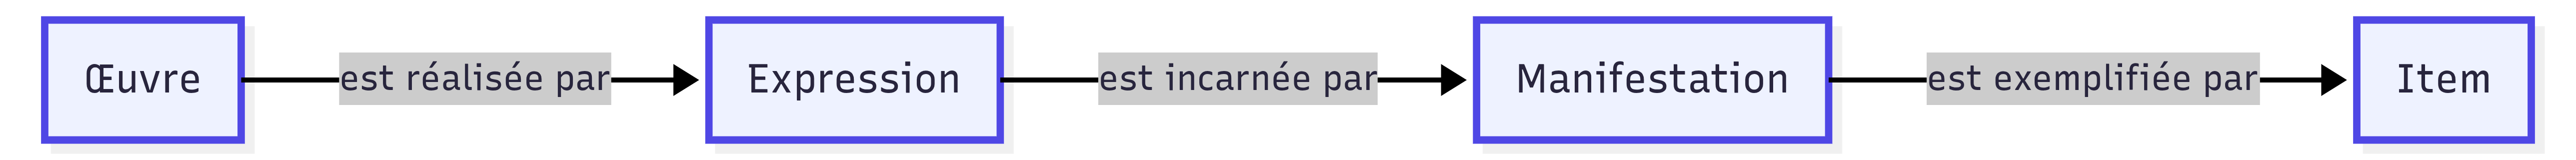
\includegraphics[width=1.0\textwidth]{images/FRBRfirstgroup.png} 
	
	\caption{Entités du modèle \gls{FRBR}} 
	
	\label{figFRBR1} 
	
\end{figure} 



Le \gls{FRBR} est qualifié de modèle entité-relation, qui modélise précisément les relations qui peuvent exister entre les différents niveaux de description et, de ce fait, entre les éléments d'un système d’information, afin de permettre à l'utilisateur de les retrouver plus facilement. Afin d’illustrer la manière dont s’articule la description d’un ouvrage bibliographique selon la modélisation proposée par le FRBR, prenons l'exemple de l'ouvrage \textit{Qu'est-ce que le cinéma} d'André Bazin. Au niveau Œuvre, est décrite l'idée intellectuelle de l'ouvrage, essentiellement matérialisée par son contexte de création. Cet ouvrage, est notamment exprimé et matérialisé au sein d'un texte intégral en quatre volumes écrit entre 1958 et 1962, dont les modalités sont décrites au niveau Expression. Cette expression de l’ouvrage est notamment publiée comme édition originale aux Editions du Cerf, dont les modalités sont décrites au niveau Manifestation. Enfin, l’exemplaire individuel de cette manifestation est potentiellement conservé dans une bibliothèque avec une côte unique, dont les caractéristiques physiques sont décrites au niveau Item. Une même œuvre peut être exprimée au sein de multiples expressions, de même qu’une expression peut faire l'objet de diverses manifestations. Le foisonnement d’éléments liés à une même œuvre peut rapidement rendre complexe la navigation de l’utilisateur au sein d’un outil de gestion des collections. La description proposée par le modèle \gls{FRBR} permet de distinguer les différentes étapes du cycle de vie d’une œuvre et ses différentes matérialisations, permettant ainsi une navigation plus fluide entre les éléments liés au sein d’un catalogue.  

Notons qu’à ces quatre entités de premier groupe Œuvre, Expression, Manifestation, Item), s'ajoutent deux entités de second groupe : Personnes et Collectivités. Elles expriment le rôle joué sur la production ou le contenu d'une ou plusieurs entités du premier groupe. \footcite{zotero-item-657} Par exemple, l'auteur est relié aux niveaux Œuvre et Expression, l'éditeur au niveau Manifestation, le catalogueur au niveau Item. 

Enfin, il existe des entités de troisième groupe intégrées au modèle, qui correspondent à des Concepts, Objets, Évènements ou Lieux liés aux entités de premier et de second groupe. \footcite{zotero-item-657} 

Réunies, les entités des trois groupes confondus modélisent une structure complexe caractérisée par les liens entre éléments, comme le montre la figure \ref{figFRBR2}  

\begin{figure}[htbp] 
	
	\centering 
	
	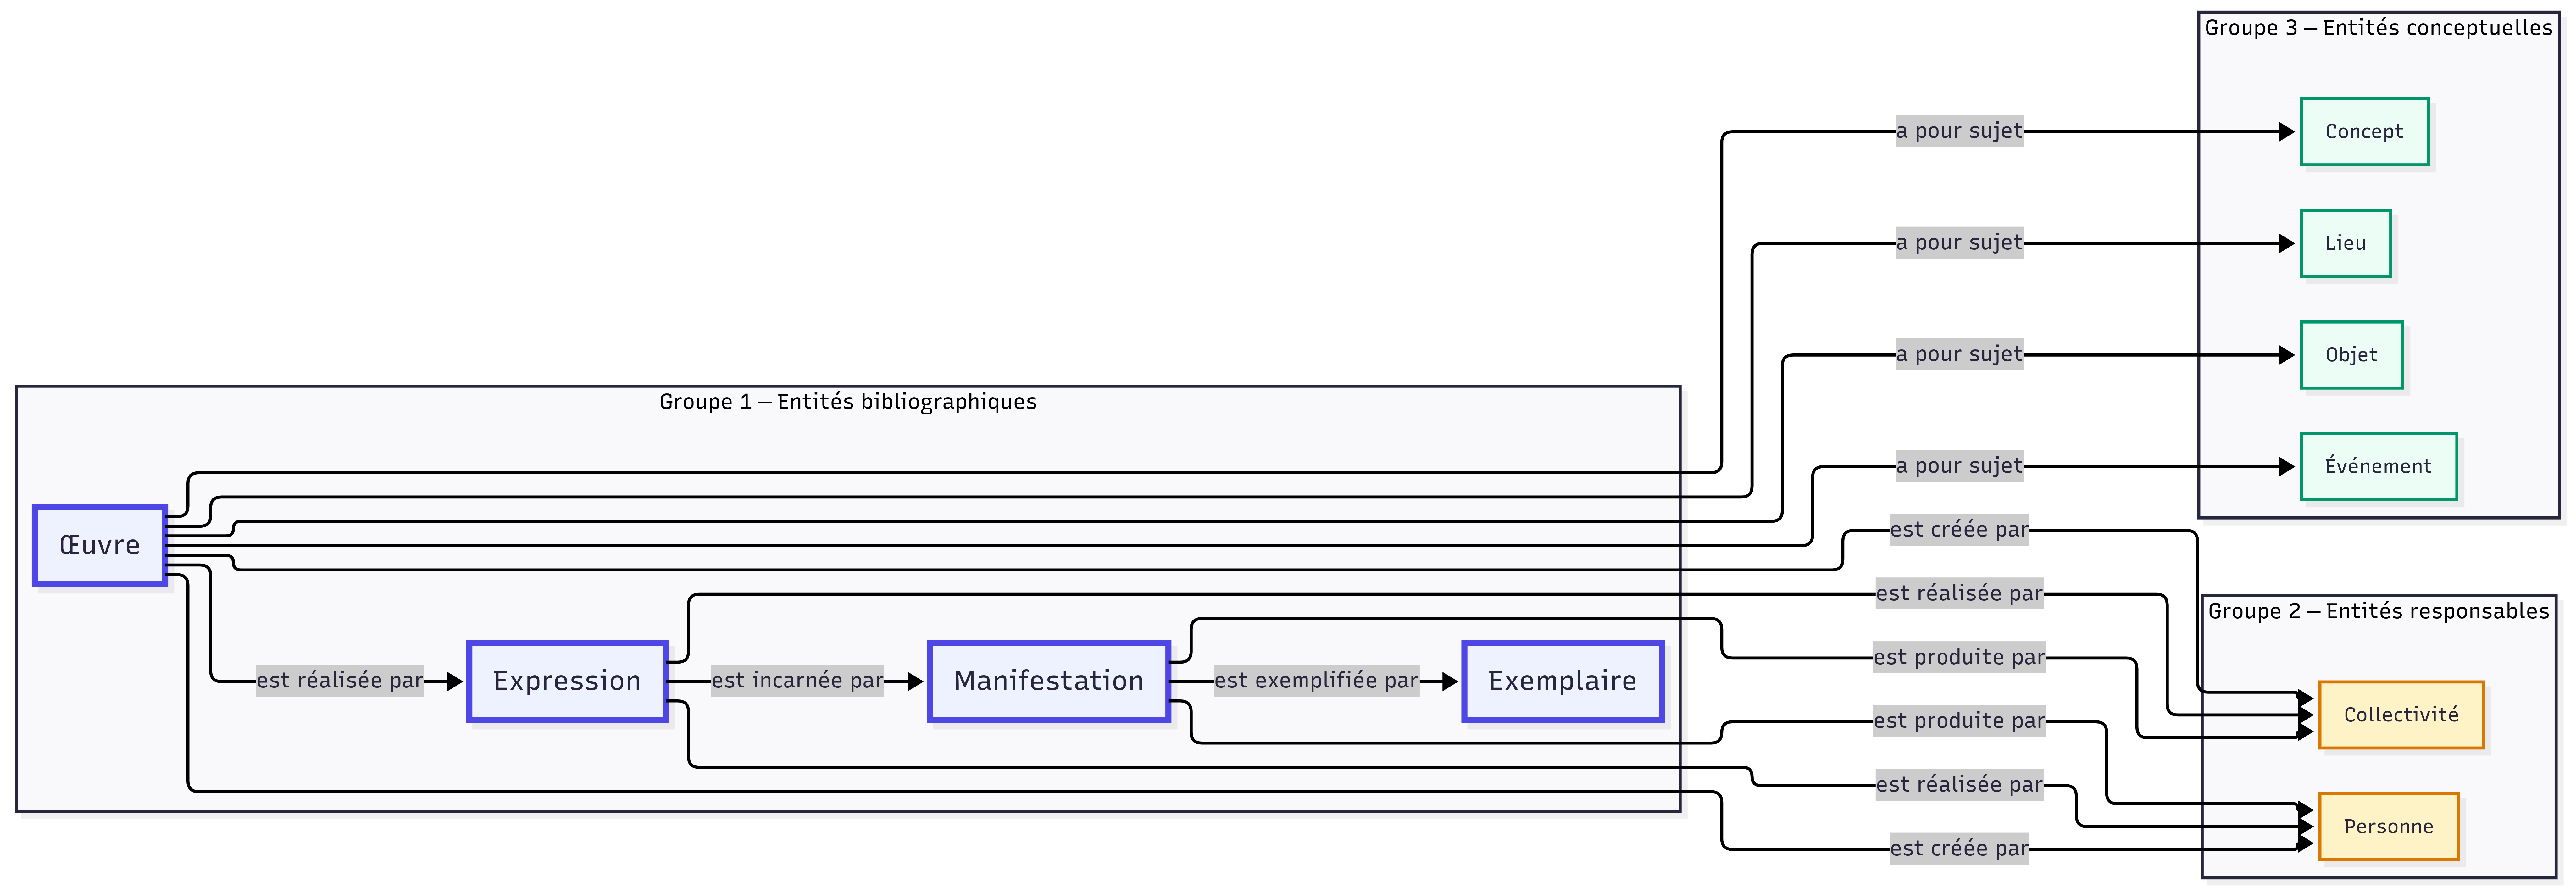
\includegraphics[width=1.0\textwidth]{images/FRBRentitesBiblio.png} 
	
	\caption{Entités du modèle FRBR} 
	
	\label{figFRBR2} 
	
\end{figure} 

Toutefois, dans le cadre de ce mémoire, nous nous concentrerons sur les entités de premier groupe, qui constituent les entités principales de description pour les archives audiovisuelles au sein du logiciel de gestion des collections créé par Skinsoft. Les entités de second et troisième groupe constituent moins des entités à part entière que des éléments de description contrôlés par des thésaurus.  

Le modèle \gls{FRBR}, fondé sur les relations entre entités, est avant tout conçu dans l’optique de faciliter la navigation de l'utilisateur au sein d'un catalogue, entre les liens qui régissent les différents éléments d'une collection.  Le \gls{FRBR} prétend en effet répondre à quatre besoins utilisateur principaux : trouver, identifier, sélectionner, obtenir. \footcite{zotero-item-653}. Il permet à l'utilisateur de localiser la ressource, d'identifier si elle correspond bien à ce qu'il cherche, de la sélectionner selon ses besoins, avant d'accéder finalement à son contenu. Nous ajouterons que le besoin fondateur de la création d'un tel modèle est également celui de pouvoir visualiser et explorer les liens de la ressource identifiée avec d'autres ressources pertinentes qui y sont directement associées. \footcite{zotero-item-653} Ce modèle de données se situerait donc à l'intersection de deux besoins principaux : celui d'améliorer la connaissance sur une ressource donnée en visibilisant ses relations, et celui d'améliorer l'expérience utilisateur en proposant une interface navigable et intuitive. 

%Donner un exemple d’institution qui utilise ce modèle et comment ça se matérialise dans un catalogue en ligne (bibliothèque kandinsky?) 

Notons que ces besoins s'appliquent non seulement à l'utilisateur faisant partie d'un public, au sein d'un catalogue ou d'une base de données en ligne, mais également à un utilisateur métier, interne à l'institution et gestionnaire des collections. C'est précisément sur les besoins métier de ce dernier que se concentre l'analyse de ce mémoire de recherche, puisque Skinsoft propose avant tout un outil de gestion des collections interne. De fait, les enjeux de l'implémentation et de l'adaptation du modèle \gls{FRBR} se situent au cœur des ambitions d'un logiciel de gestion des collections, dont l’objectif est d’améliorer l’interface afin d’assurer l’efficacité de l’utilisateur métier.  







%L'adoption de ces modèles dans les catalogues est réalisé dans l'objectif d'améliorer la visibilité des données au sein du web de données et donner accès au public aux données produites, même si ce mémoire se concentre sur l'utilisateur métier. (définir le web de données?) \footcite{zotero-item-661} 
\section{\label{I_1_B}Son adaptation à l'archivistique et au contexte muséal}

Le modèle \gls{FRBR} est un modèle conçu par et pour les bibliothèques. À ce jour, les bibliothèques n'utilisent plus seulement le modèle FRBR mais la somme du FRBR et de ses modèles étendus : le \gls{FRAD} (Fonctionnalités requises des données d'autorité) pour la description des autorités, et le FRSAD (Fonctionnalités requises des données d'autorité matière) pour la description des sujets.\footcite{zotero-item-651}. La somme de ces modèles constitue le modèle \gls{IFLA-LRM}, successeur du \gls{FRBR}. Le modèle \gls{FRBR} est toutefois largement utilisé dans le domaine de la gestion des collections muséales. Or, sa qualité de modèle ne prétend pas normaliser la description des données, seulement d’en cadrer l’affichage. De fait, les entités proposées par le modèle \gls{FRBR} peuvent paraître génériques, et doivent être soumises à une redéfinition à chaque implémentation selon le contexte donné \footcite{boeuf2008}. Cette flexibilité ne doit toutefois pas nuire à l'objectif principal, celui de faciliter la navigation de l'utilisateur, en explicitant les “interrelations" entres les notices et les données produites \footcite{boeuf2008}. Nous étudierons dans les chapitres suivants une double adaptation, celle du modèle \gls{FRBR} à d’autres types de documents : objets de collections et archives, et son adaptation à différents contextes institutionnels pour une même nature de documents, celle des archives audiovisuelles.  

%Analysons premièrement son adaptation au milieu archivistique. La difficulté principale de l'adaptation du modèle FRBR aux collections d'archives est que le niveau Œuvre ne peut contenir le plus haut niveau archivistique : le fonds d'archives. En effet, un fonds d'archive ne peut être considéré systématiquement comme une œuvre, puisque dans la plupart des cas, il s'agit plutôt d'une agrégation naturelle d'éléments quotidiens produits par une personne morale ou physique. Ainsi, un fonds d'archives ne peut être intégré à la définition d'une œuvre comme création intellectuelle et artistique distincte \footcite{fick2015}. Un fonds d'archives correspondrait davantage à un agrégat d'œuvres ou de travaux, niveau intermédiaire décrit par le modèle FRBR : "un ensemble de documents privés classés par des archives en un seul fonds"(traduction). \footcite{fick2015}. Le niveau manifestation est obsolète car les archives ne sont pas publiées ?  

%Développer un peu plus sur l’adaptation du modèle aux archives : qu’en est-il des autres niveaux ? À quoi ressemble un catalogue d’une institution qui utilise le FRBR pour les archives ? (À relier avec le sujet) 

Le modèle de données \gls{FRBR} a été adapté au milieu muséal à travers une version orientée objet, le \gls{FRBRoo}, extension du \gls{CIDOC-CRM} (object-oriented Conceptual Reference Model), l'ontologie de référence dédiée au patrimoine culturel et muséal \footcite{gillis2015}. Il s’agit d’un modèle conceptuel général visant l’interopérabilité entre les données provenant d’institutions diverses dont les musées, centres d’archives et bibliothèques.  

Ce dernier modélise une approche descriptive centrée sur les évènements entourant l’objet décrit. Ainsi, les entités bibliographiques ne sont plus seulement décrites par des attributs, mais par des évènements spatio-temporels qui les créent et les font évoluer selon différents contextes \footcite{dialogue2017} Cette adaptation du \gls{FRBR} est particulièrement pertinente pour la description de collections de musées composites et de différentes natures, pouvant englober à la fois la description de tableaux, sculptures, ouvrages, specimens, films, etc. Tandis que le \gls{FRBR} est modélisé à partir de la nature d’un document bibliographique le FRBRoo replace la description dans un contexte plus large, celui d’évènements situés dans l’espace et dans le temps, évènements qui peuvent agir sur n’importe quel type d’objet.  

Le \gls{FRBRoo} est un modèle intéressant pour la gestion des archives audiovisuelles. En effet, les \gls{Archivesaudiovisuelles} possèdent un statut hybride au sein d’institutions patrimoniales, relevant à la fois de la création artistique, de l’œuvre et d’un archivage du réel, d’un témoignage \footcite{zotero-item-669}. Le \gls{FRBRoo} propose deux entités pertinentes, qui pourraient permettre de distinguer l’évolution de ce double statut : l’œuvre (Individual work), et la captation ou l’enregistrement (Recording work). Par exemple, l’étape du tournage serait documentée par l’entité Captation ainsi que l'ensemble des évènements et des personnes qui y sont liés, alors que le montage serait documenté par l’entité Œuvre ainsi que les évènements et les personnes qui y sont liés. Le FRBRoo conserve ensuite les entités prévues par le FRBR : l’Expression, la Manifestation, l’Item.  

Néanmoins, si le FRBRoo constitue une adaptation pertinente du FRBR pour le milieu muséal, sa structure trop large ne permet pas de rendre compte la nature propre du médium cinématographique, qui fonde la gestion des collections audiovisuelles. Ainsi, les institutions préservatrices de collections audiovisuelles se tournent davantage vers des adaptations métier spécifiques, comme celle de la fédération des archives du film (FIAF). La FIAF propose en effet une application du FRBR spécifique aux usages métier de description des archives audiovisuelles, au sein d’un manuel de catalogage des images animées. 

\section{\label{I_1_C}Un modèle adapté aux archives audiovisuelles : le manuel de catalogage des images animées de la FIAF } 

L’adaptation du modèle FRBR aux archives audiovisuelles impose une double redéfinition : elle doit prendre en compte d’une part la nature propre du langage cinématographique, et d’autre part, les spécificités des corpus audiovisuels conservés. La modélisation en différentes couches de description prévue par le FRBR est pertinente pour le cinéma, qui partage avec le milieu bibliographique un mode de production industriel, permettant ainsi de distinguer la création intellectuelle de ses copies et diffusions multiples. Toutefois, les niveaux bibliographiques classiques dits WEMI (Work, Expression, Manifestation, Item) restent limitées pour la description métier des spécificités des archives audiovisuelles.  

Premièrement, alors que les bibliothèques conservent principalement des copies identiques d’une même publication, les archives d’images animées sont fréquemment amenées à gérer des objets uniques et rares tels que des \textit{rushes}, des films amateurs, montages inachevés, copies annotées, etc. \footcite{zotero-item-646}. Pour ce type de collections, le niveau Manifestation devient obsolète, en raison du caractère inédit de leur création. Deuxièmement, la distinction du FRBR bibliographique entre l’Œuvre (l’idée de création), et l’Expression (sa réalisation) s’adapte mal au contexte cinématographique. En effet, un film prend véritablement forme au moment du tournage puis du montage, rendant ainsi l’idée d’une existence abstraite de création en amont, caduque. Il parait alors plus pertinent d’appréhender l’œuvre cinématographique moins comme une entité abstraite en amont de son expression que comme une entité concrète ancrée dans un processus d’expression.  

Afin de répondre à ces contraintes imposées par le processus de création cinématographique, la FIAF a élaboré un manuel de catalogage des images animées \footcite{zotero-item-644}. Le manuel adapte le modèle FRBR en le combinant aux règles descriptives RDA (Ressources, Description, Accès) dédiées aux archives, et aux normes de description des œuvres cinématographiques (EN 15744 / EN 15907) \footcite{zotero-item-646}. Le manuel se focalise sur les entités de premier groupe afin d’en repenser l’articulation et de proposer de remplacer le schéma WEMI par le schéma WVMI (Work, Variant, Manifestation, Item).  

En effet la FIAF propose de fusionner le niveau Expression dans celui de l'Œuvre, permettant alors à l’Œuvre de regrouper la description intellectuelle et le processus de création de l’archive cinématographique. Par exemple, si nous prenons le film \textit{L'Aigle à deux têtes} (France, 1948, réalisé par Jean Cocteau), le niveau Oeuvre permettrait d’y décrire le contexte de création ainsi que le contenu. De plus, la FIAF propose une nouvelle entité, celle de Variante, optionnelle, qui se substitue à celle d’Expression. Elle permet de décrire toute version différente d’une œuvre originale dans la mesure où son sens principal n’est pas altéré. Par exemple, une version d’un film qui serait colorisée, censurée, doublée, remontée, etc. Si nous reprenons \textit{L'Aigle à deux têtes}, une variante possible est celle de la restauration du film en 4K en 2023, dont le niveau Variante permettrait de décrire les variations portées sur l’œuvre. La FIAF conserve par ailleurs le niveau de Manifestation, toutefois redéfini afin de pouvoir décrire la matérialisation physique ou numérique d’une Œuvre ou de sa Variante sur un support, ainsi que son contexte de diffusion. Par exemple, la manifestation de la version restaurée de \textit{L'Aigle à deux têtes} décrirait la sortie de cette version en Blu-Ray et DVD chez Rimini Editions. Enfin, le niveau Item est également conservé afin de décrire l’exemplaire physique ou le fichier numérique unique issu de la Manifestation d’une Œuvre ou de sa Variante. Cet exemplaire est concrètement préservé et géré par l’institution et décrit par des métadonnées de conservation.  

Cette restructuration du FRBR permet ainsi de répondre aux besoins métiers spécifiques de gestion de collections d’images animées. Selon la FIAF, la modélisation de cette réadaptation du FRBR au sein d’un outil de gestion des collections devrait permettre aux utilisateurs métier “d’identifier, sélectionner et acquérir” efficacement toutes les variantes d’une œuvre, l’ensemble des manifestations d’une version d’une œuvre, les exemplaires physiques disponibles d’une manifestation d’une œuvre \footcite{zotero-item-646}. La FIAF reprend ainsi les besoins utilisateurs fondateurs de la structuration du FRBR bibliographique en les adaptant à une nécessité de pouvoir circuler entre les différentes versions d’une œuvre à différents stades du processus de l’industrie cinématographique.  

Toutefois, l’implémentation d’un tel modèle au sein d’un outil de gestion des collections se heurte aux spécificités des différents corpus audiovisuels, dont certains ne possèdent pas de manifestation par exemple. En effet, si le modèle s'applique adéquatement aux corpus de cinéma dits "classiques" dont la chaîne de production industrielle est respectée : un film est réalisé à l'issue d'un tournage et d'un montage (Œuvre), puis distribué (Manifestation), et copié en multiples exemplaires (Item). Or, dans le cas de corpus spécifiques, expérimentaux, personnels, ou amateurs, qui font l’objet de descriptions complexes, la modélisation FRBR classique s'avère limitée. Ce type de corpus est notamment peu distribué ou diffusé, rendant notamment le niveau de Manifestation obsolète. 

Ainsi, le FRBR reste un modèle qu’il s’agit de réadapter à chaque contexte institutionnel \footcite{boeuf2008}. Le manuel de la FIAF agit comme un cadre théorique de structuration de la description pour la globalité des archives audiovisuelles, qui subit une redéfinition pour chaque type de corpus audiovisuel : amateur, commercial, documentaire, grand public, etc.  

Reproductibilité technique ? \footcite{zotero-item-669} 






		
		
		
		%le but ultime de la modélisation des données et de leur structuration est leur interopérabilité et leur versement sur le web de données par les institutions qui le souhaitent. Permet de passer de la donnée brute à l'information intelligible. dès l'inventaire des données, la modélisation doit être prise en compte et également le multilinguisime pour faciliter l'ouverture des données. \footcite{chambonnet} 
		
		%Nécessité d'uniformiser même si les corpus sont hétérogènes pour assurer l'intéropérabilité des données.  
		
		%Transition vers la deuxième sous partie : adapter le FRBR aux archives audiovisuelles 
		
		
		
		%à replacer - fin de la deuxième sous partie :  
		
		%Transition entre le modèle de données et l'automatisation :  
		
		%justification de la clarté du modèle FRBR pour la mise en place d'un modèle automatique :  
		
		% 
		
		%Impact de l'indexation automatique sur les données : 
		
		% 
		
		%"Comme le repérage d’entités visuelles demande énormément d’informations locales, les bases de données d’indexation constituées à partir de la reconnaissance des entités sont conséquentes (elles peuvent avoir une taille supérieure à celle des vidéos elles-mêmes) et font l’objet de recherches au sein de l’établissement pour en optimiser les temps de calcul. Dans ce contexte, la qualité et la modélisation des données jouent un rôle fondamental car c’est sur les bases de données que les algorithmes sont entrainés."\footcite{moiraghi2018} 
		
		% 
		
		%Nous prenons ici la pensée inverse, ce n'est pas seulement l'indexation automatique qui nécessite un modèle de données qualitatif, mais nous réfléchissons justement à la manière dont le modèle de données façonne l'indexation automatique et la manière dont l'indexation automatique permet de repenser le modèle de données dans lequel est implémentée.  
		
		% 


\chapter{\label{I_2}Implémenter le FRBR adapté aux archives audiovisuelles au sein d’un outil de gestion des collections} 

%I 2 

%Reprendre la définition du logiciel de gestion des collections ? Pour montrer que le FRBR aide à la gestion des collections 

Comme défini en introduction, un logiciel de gestion des collections est un outil “spécialisé permettant de gérer des informations structurées” \footcite{zotero-item-766}. De ce fait, il structure le système d’information qui permet à une institution d’orchestrer le cycle de vie de sa collection. Cette structuration des données doit être modélisée selon les spécificités propres au type de collection d’un institution cliente, à partir de normes descriptives définies et de cadres de référence pour l’indexation des collections. Dans le cas des archives audiovisuelles, le logiciel des gestions des collections devrait ainsi permettre une structuration de l’information adaptée au type de corpus conservé, respectant toutefois le cadre de référence pour la modélisation des données, le FRBR. La restructuration du modèle de données permet de construire pour l’utilisateur, un logiciel de gestion des collections intelligible avec des outils de recherche performants. (En accord avec les besoins utilisateurs FRBR)  


\section{\label{I_2_A}Un espace de travail dédié à la gestion de collections audiovisuelles : S-Movies}

Si le manuel de la FIAF pose le cadre d’une adaptation du modèle FRBR pour la gestion des archives audiovisuelles, il s'agit désormais de confronter ce cadre à une implémentation concrète. Pour cela, nous analyserons au cours de ce chapitre l’implémentation d’une telle modélisation au sein d’un outil de gestion des collections, celui développé par Skinsoft. Nous y analyserons spécifiquement l’espace de travail développé pour la gestion des archives audiovisuelles : S-Movies. En effet, le contexte de notre étude se situe principalement dans le cadre de l’analyse de cet espace de travail afin d’en analyser la modélisation, en vue de l’améliorer et d’y implémenter potentiellement des fonctionnalités automatiques, fondées sur l’intelligence artificielle.  

Présentons d’abord le fonctionnement général de l’outil de gestion des collections développée par Skinsoft. Celui-ci est divisé en espaces de travail, chacun dédiés à un type de collection, comme le montre la capture d'écran de la page d'accueil ci-dessous (\ref{figAccueil}). (dire en note de bas de page que les captures viennent d’une appli de test configurée par nos soins)

\begin{figure}[htbp] 
	
	\centering 
	
	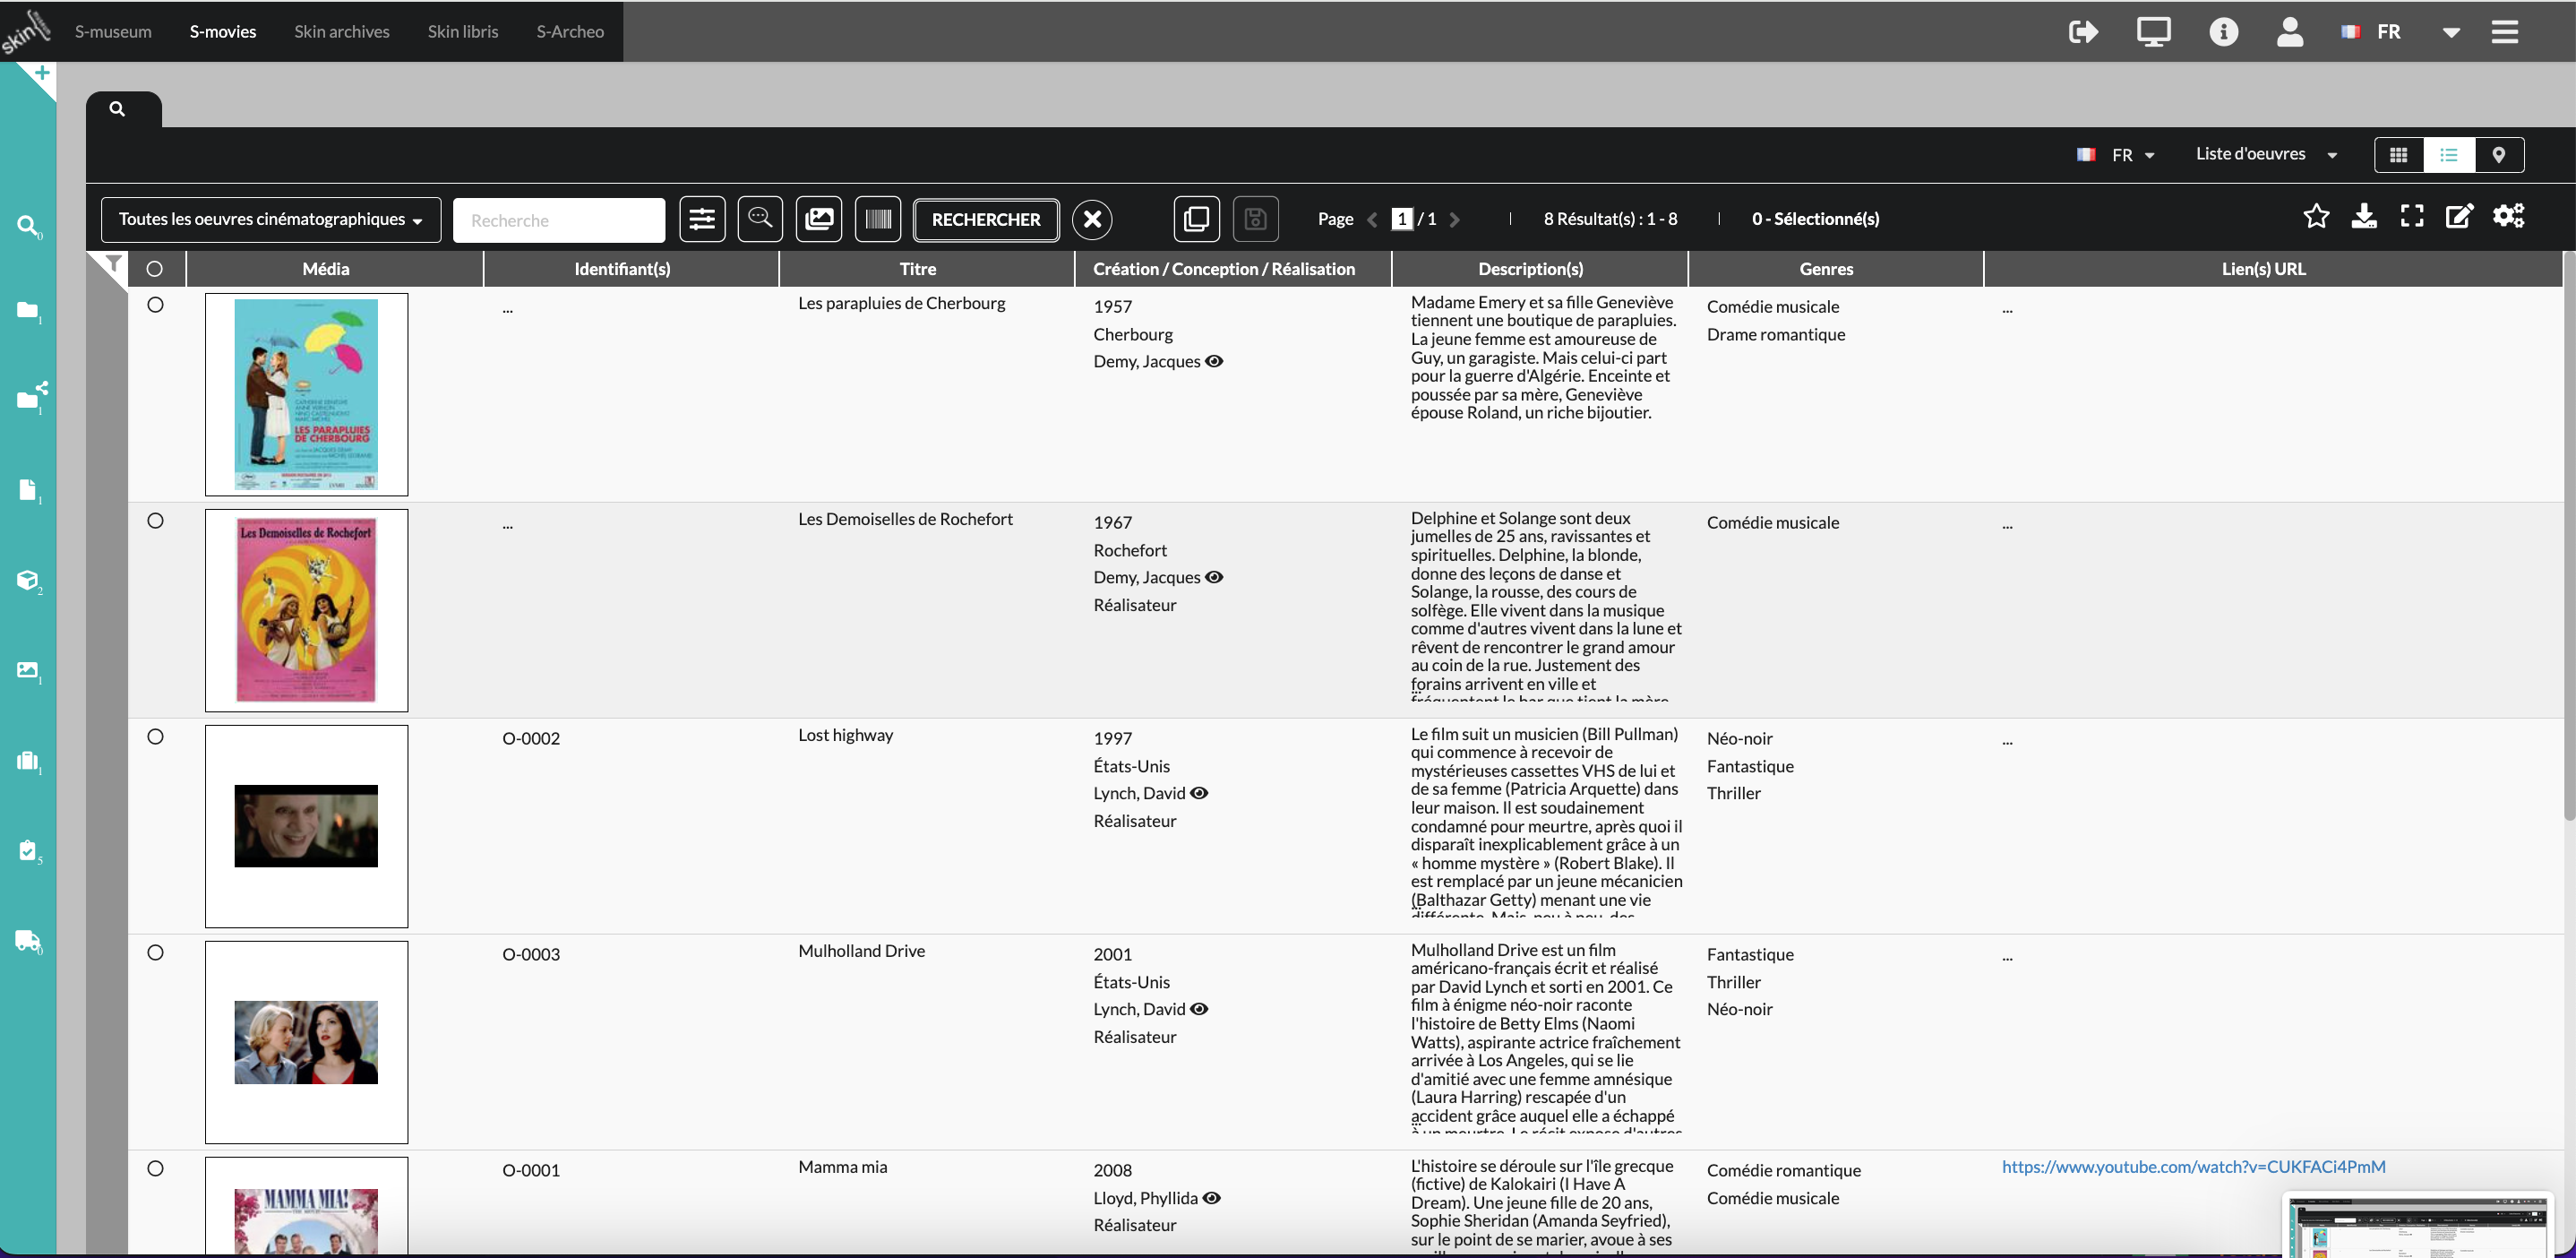
\includegraphics[width=0.85\textwidth]{images/image.png} 
	
	\caption{Page d'accueil de l'espace de travail} 
	
	\label{figAccueil} 
	
\end{figure}

Une institution cliente de l’outil peut combiner un ou plusieurs espaces de travail, selon les données à gérer. Cette structure permet justement d’adapter l’interface à chaque type de collection géré : objets de collection de musée, collections archéologiques, collections de films, collections bibliographiques, collections d’archives, etc. Chaque espace de travail permet notamment la gestion des acquisitions, des collections, de leurs mouvements, de projets, d’expositions, des médias... De plus, chaque espace de travail est structuré selon des normes de description et un cadre de modélisation adaptés au type de collection qui y est géré. L'espace de travail S-Movies est modélisé selon les préconisations de la FIAF sur l’adaptation du FRBR, et structuré selon les normes de descriptions évoquées. Ainsi, les collections sont organisées en trois entités distinctes, conformément aux adaptations du FRBR par la FIAF : Films, Manifestations, Œuvres cinématographiques (Films désigne ici le niveau Item), comme le montre la capture d'écran du menu de l'espace de travail, ci-dessous :   

\begin{figure}[htbp] 
	
	\centering 
	
	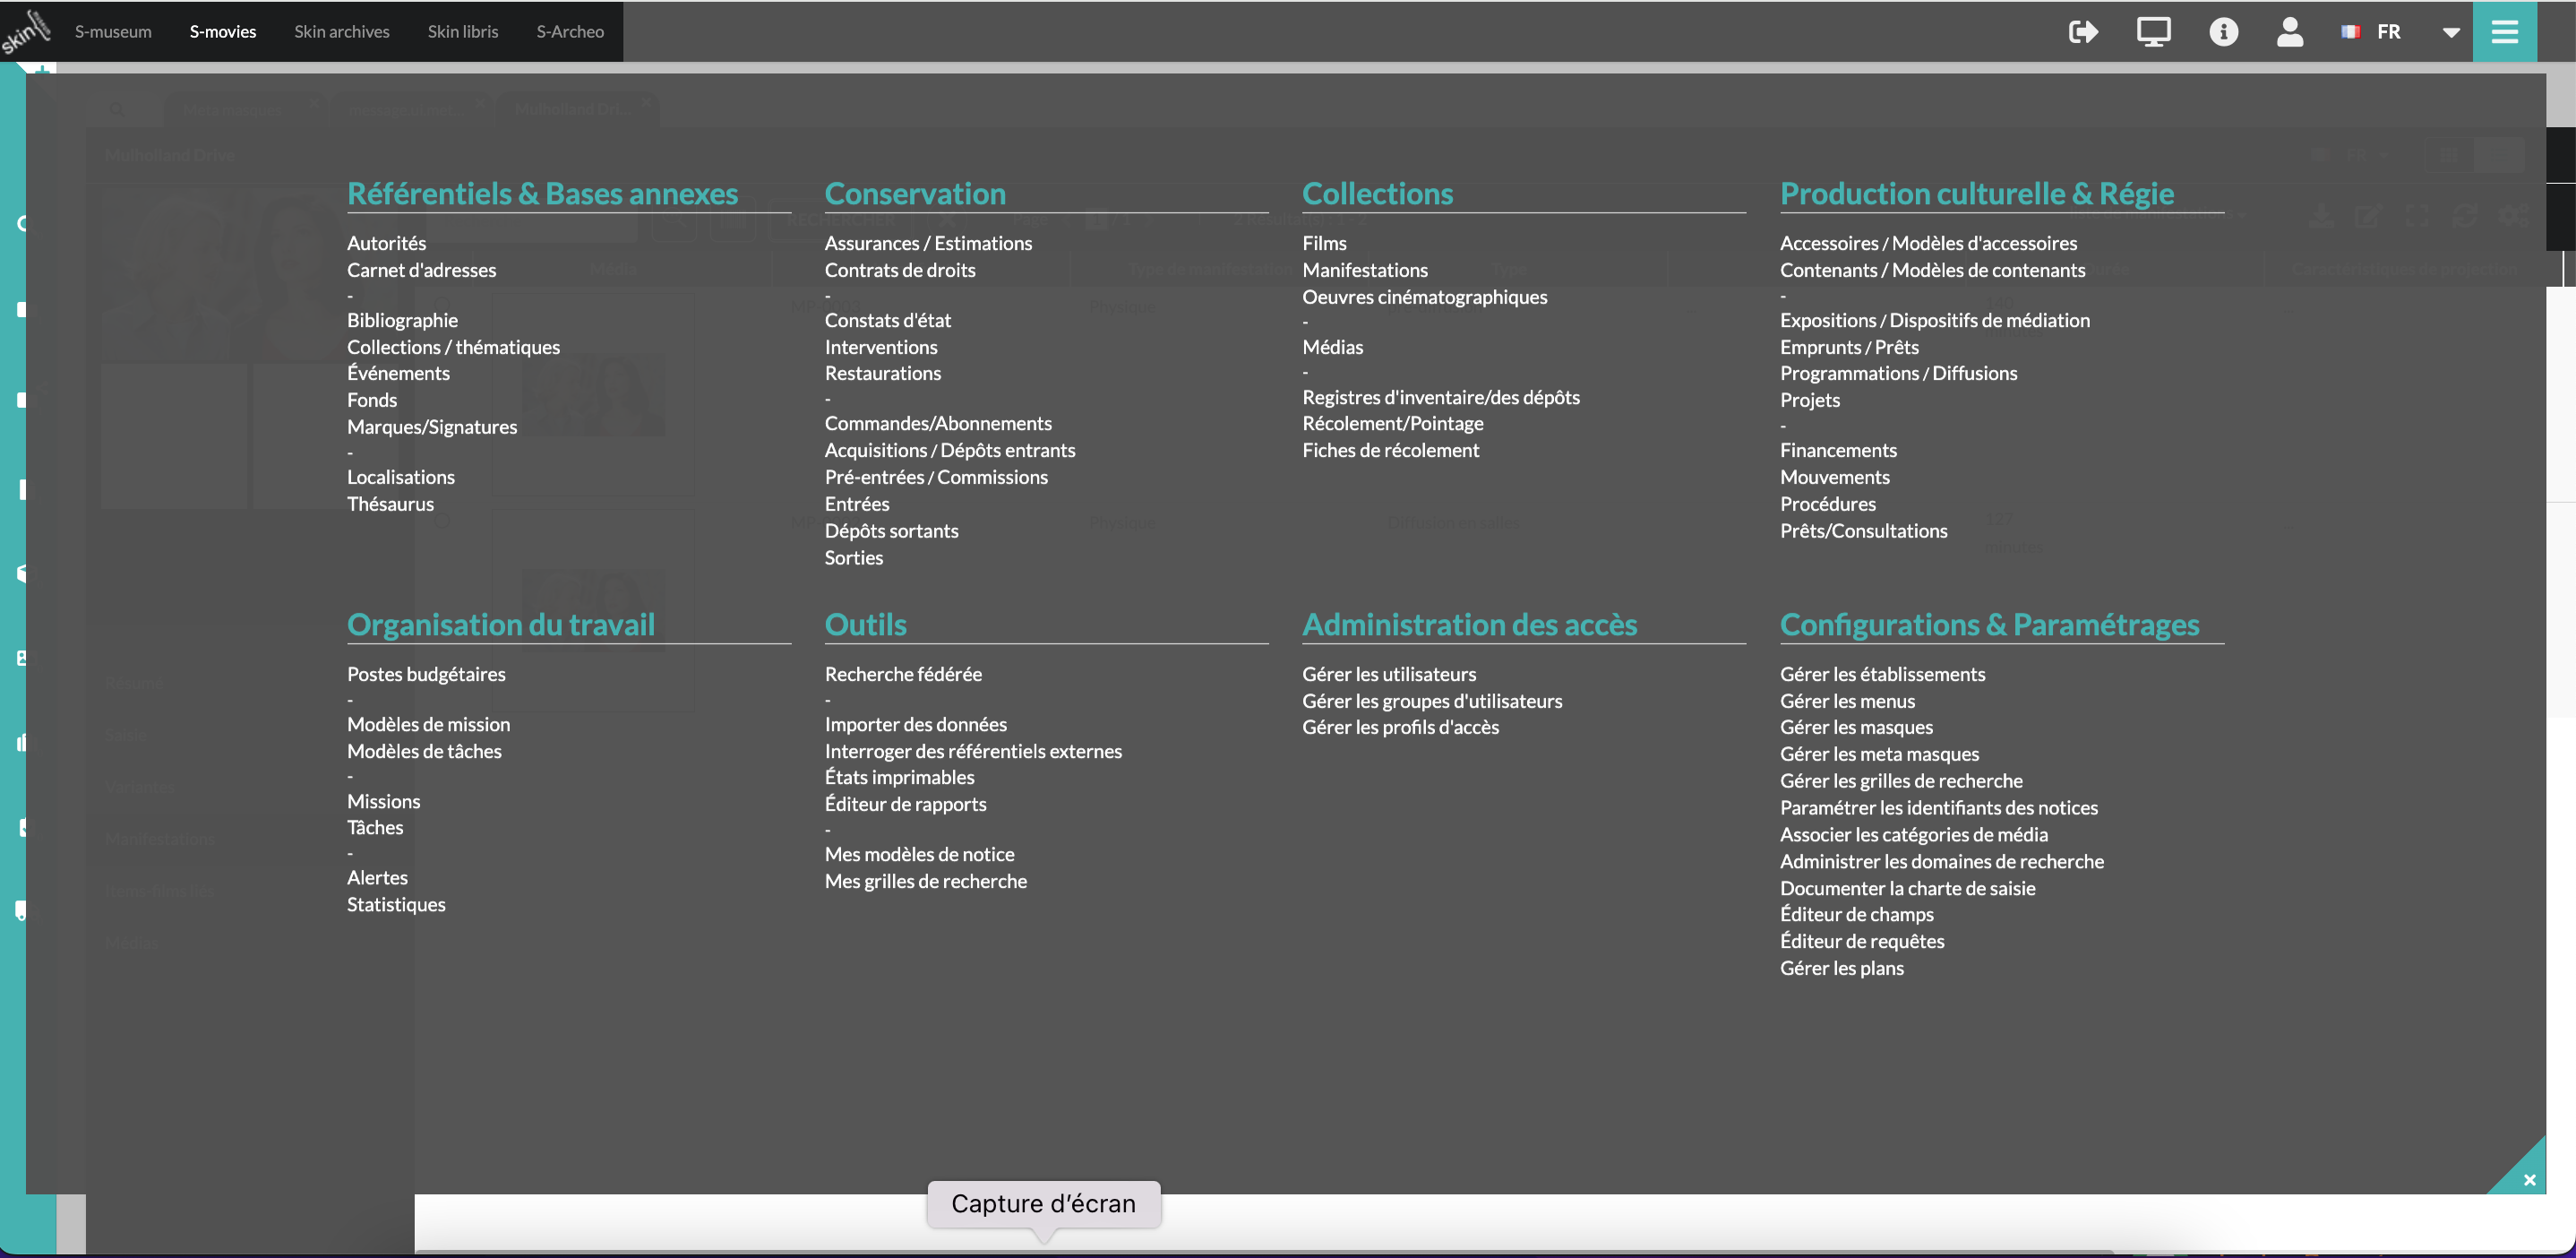
\includegraphics[width=0.85\textwidth]{images/image6.png} 
	
	\caption{Menu burger de l'espace de travail} 
	
	\label{figMenu} 
	
\end{figure}

Dans chacune de ces tables de données, l'utilisateur peut créer de nouvelles notices, et y associer des notices des autres tables. Par exemple, depuis la table Œuvres cinématographiques, l'utilisateur peut créer une notice d’Œuvre et y associer des notices de Manifestations et d'Items qui y sont directement liées. La Variante telle que définie dans le manuel de la FIAF n’est pas représentée par une entité à part entière sous la forme d’une table comme c’est le cas pour les autres entités. Toutefois, il est possible de créer une notice de Variante au sein de la table Œuvres cinématographiques, directement liée à une Œuvre. La Variante aura le même statut qu’une Oeuvre, mais elle sera de type Variante.  

Par exemple ci-dessous, une notice d’Œuvre cinématographique à laquelle sont associées deux notices de Manifestation :  

\begin{figure}[htbp] 
	
	\centering 
	
	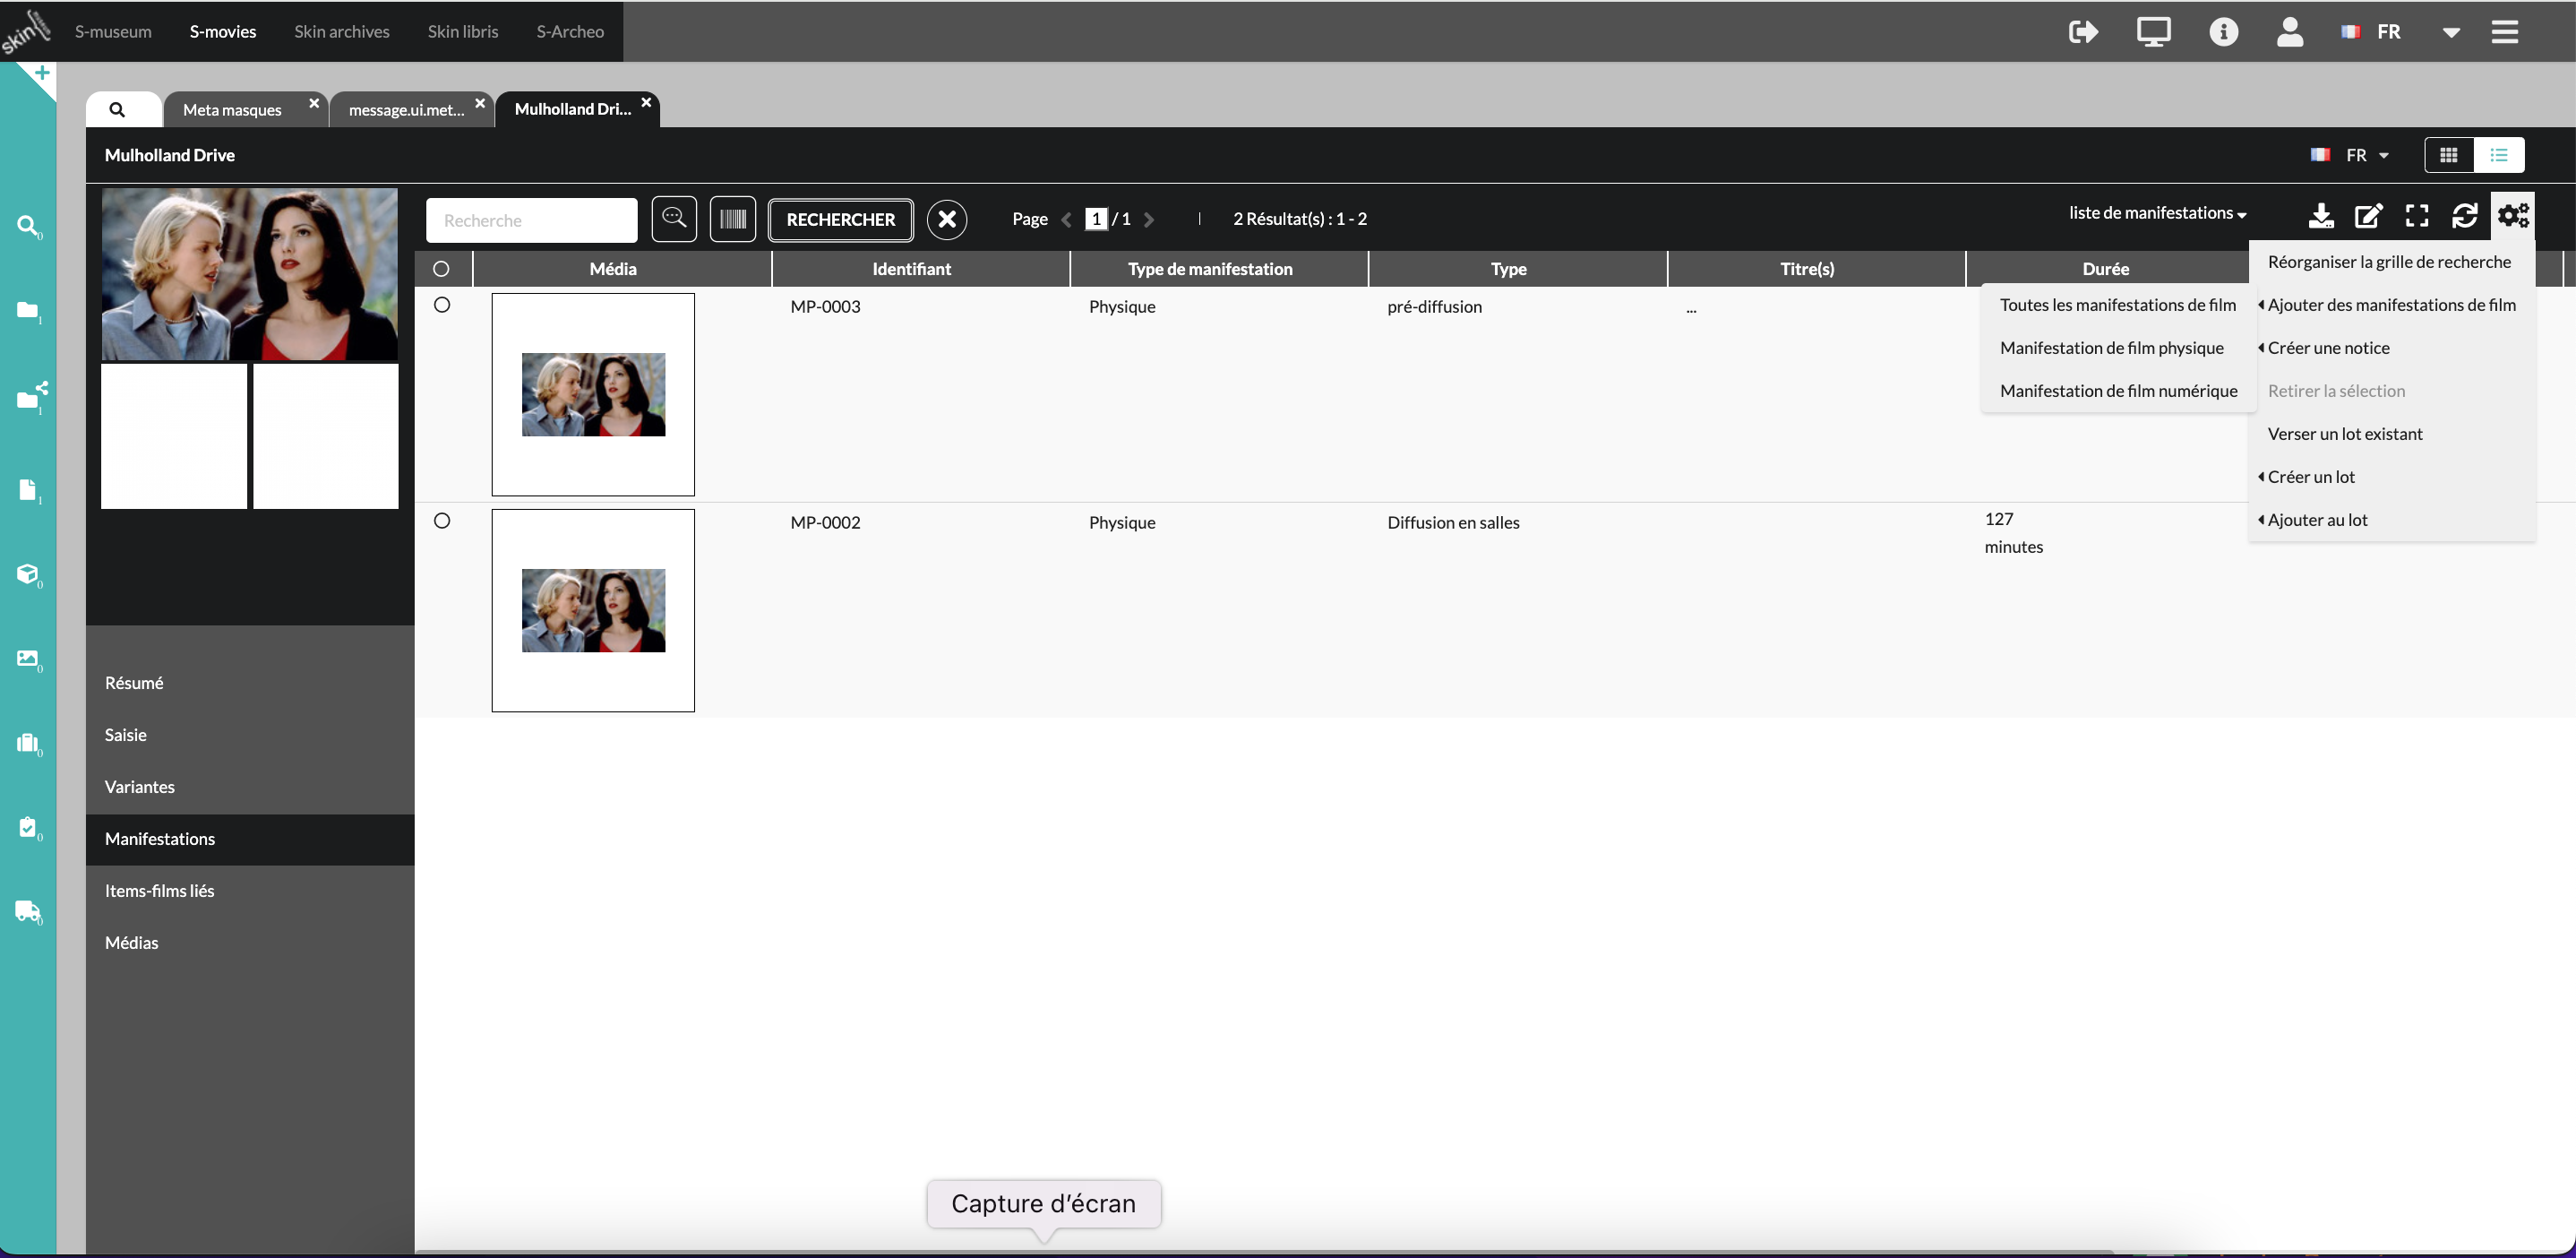
\includegraphics[width=1.0\textwidth]{images/image7.png} 
	
	\caption{Menu burger de l'espace de travail} 
	
	\label{figNoticeOeuvre} 
	
\end{figure}

L’interface permet d’associer des notices depuis un bouton d’action situé à droite.  

De plus, en fonction de la nature du corpus géré, un paramétrage adaptatif est prévu afin d’ajuster l’interface aux pratiques métier de chaque institution. En effet, une adaptation supplémentaire de la modélisation de données via la configuration flexible de chacun des espaces de travail. Trois configurations sont principalement possibles : le paramétrage de champs de saisie pour chaque type de notice, l'organisation de ces champs dans des grilles de résultats de recherche, et l'assemblage des champs et des grilles de recherche dans des menus navigables pour chaque type de notice. (Schémas explicatifs ?) Ce paramétrage concrétise la modélisation de données selon le cadre de référence utilisé.  

%quel rôle joue la modélisation dans ce cas ? En amont du paramétrage ? Ou en aval ? (Reprendre la définition) ou tout ce paramétrage fait partie de la modélisation  

Ainsi, une double adaptabilité est proposée : d’une part un espace dédié à un type de collection et structuré en fonction des normes de description et de la modélisation de données préférée, et d’autre part un paramétrage précis de l’espace de travail, propre au type de corpus géré par l'institution cliente, concrétisant ainsi la modélisation de données propre qui sera utilisée.  

L’espace de travail S-Movies est pré structuré suivant la modélisation FRBR préconisée par la FIAF. Cette structure stable, permet à Skinsoft de proposer un espace de travail pré défini pour chaque institution préservatrice de ce type de collection. En revanche, les corpus audiovisuels préservés par différentes institutions peuvent être de toutes sortes, sur différentes thématiques, sous différents formats. Cette hétérogénéité suppose des règles métiers spécifiques, issues des besoins de gestion de la collection préservé. Ainsi, par exemple, une collection audiovisuelle expérimentale ou amateure ne nécessitera pas les mêmes champs de saisie, les mêmes thésaurus, ou de la même disposition des résultats de recherche, qu'une collection audiovisuelle industrielle, grand public.   

Concrètement, au sein de l’espace de travail, la description d’un élément s’effectue au sein de champs de saisie, sélectionnés de manière adaptée aux besoins de description de l’institution donnée. Ces champs, s'ils sont paramétrables individuellement, font en réalité partie d'une structure plus large, à l'échelle de l'espace de travail dans lequel ils se situent. En effet, ces champs sont regroupés dans des masques, qui correspondent à des formulaires de saisie spécifiques au type de notice concerné. Par exemple, une notice de film physique, décrivant le niveau Item pourra contenir un masque de saisie, contenant des champs de saisie correspondants (cf \ref{figMasques}): identifiants, format de l’item, support de l’item, etc. 

\begin{figure}[htbp] 
	
	\centering 
	
	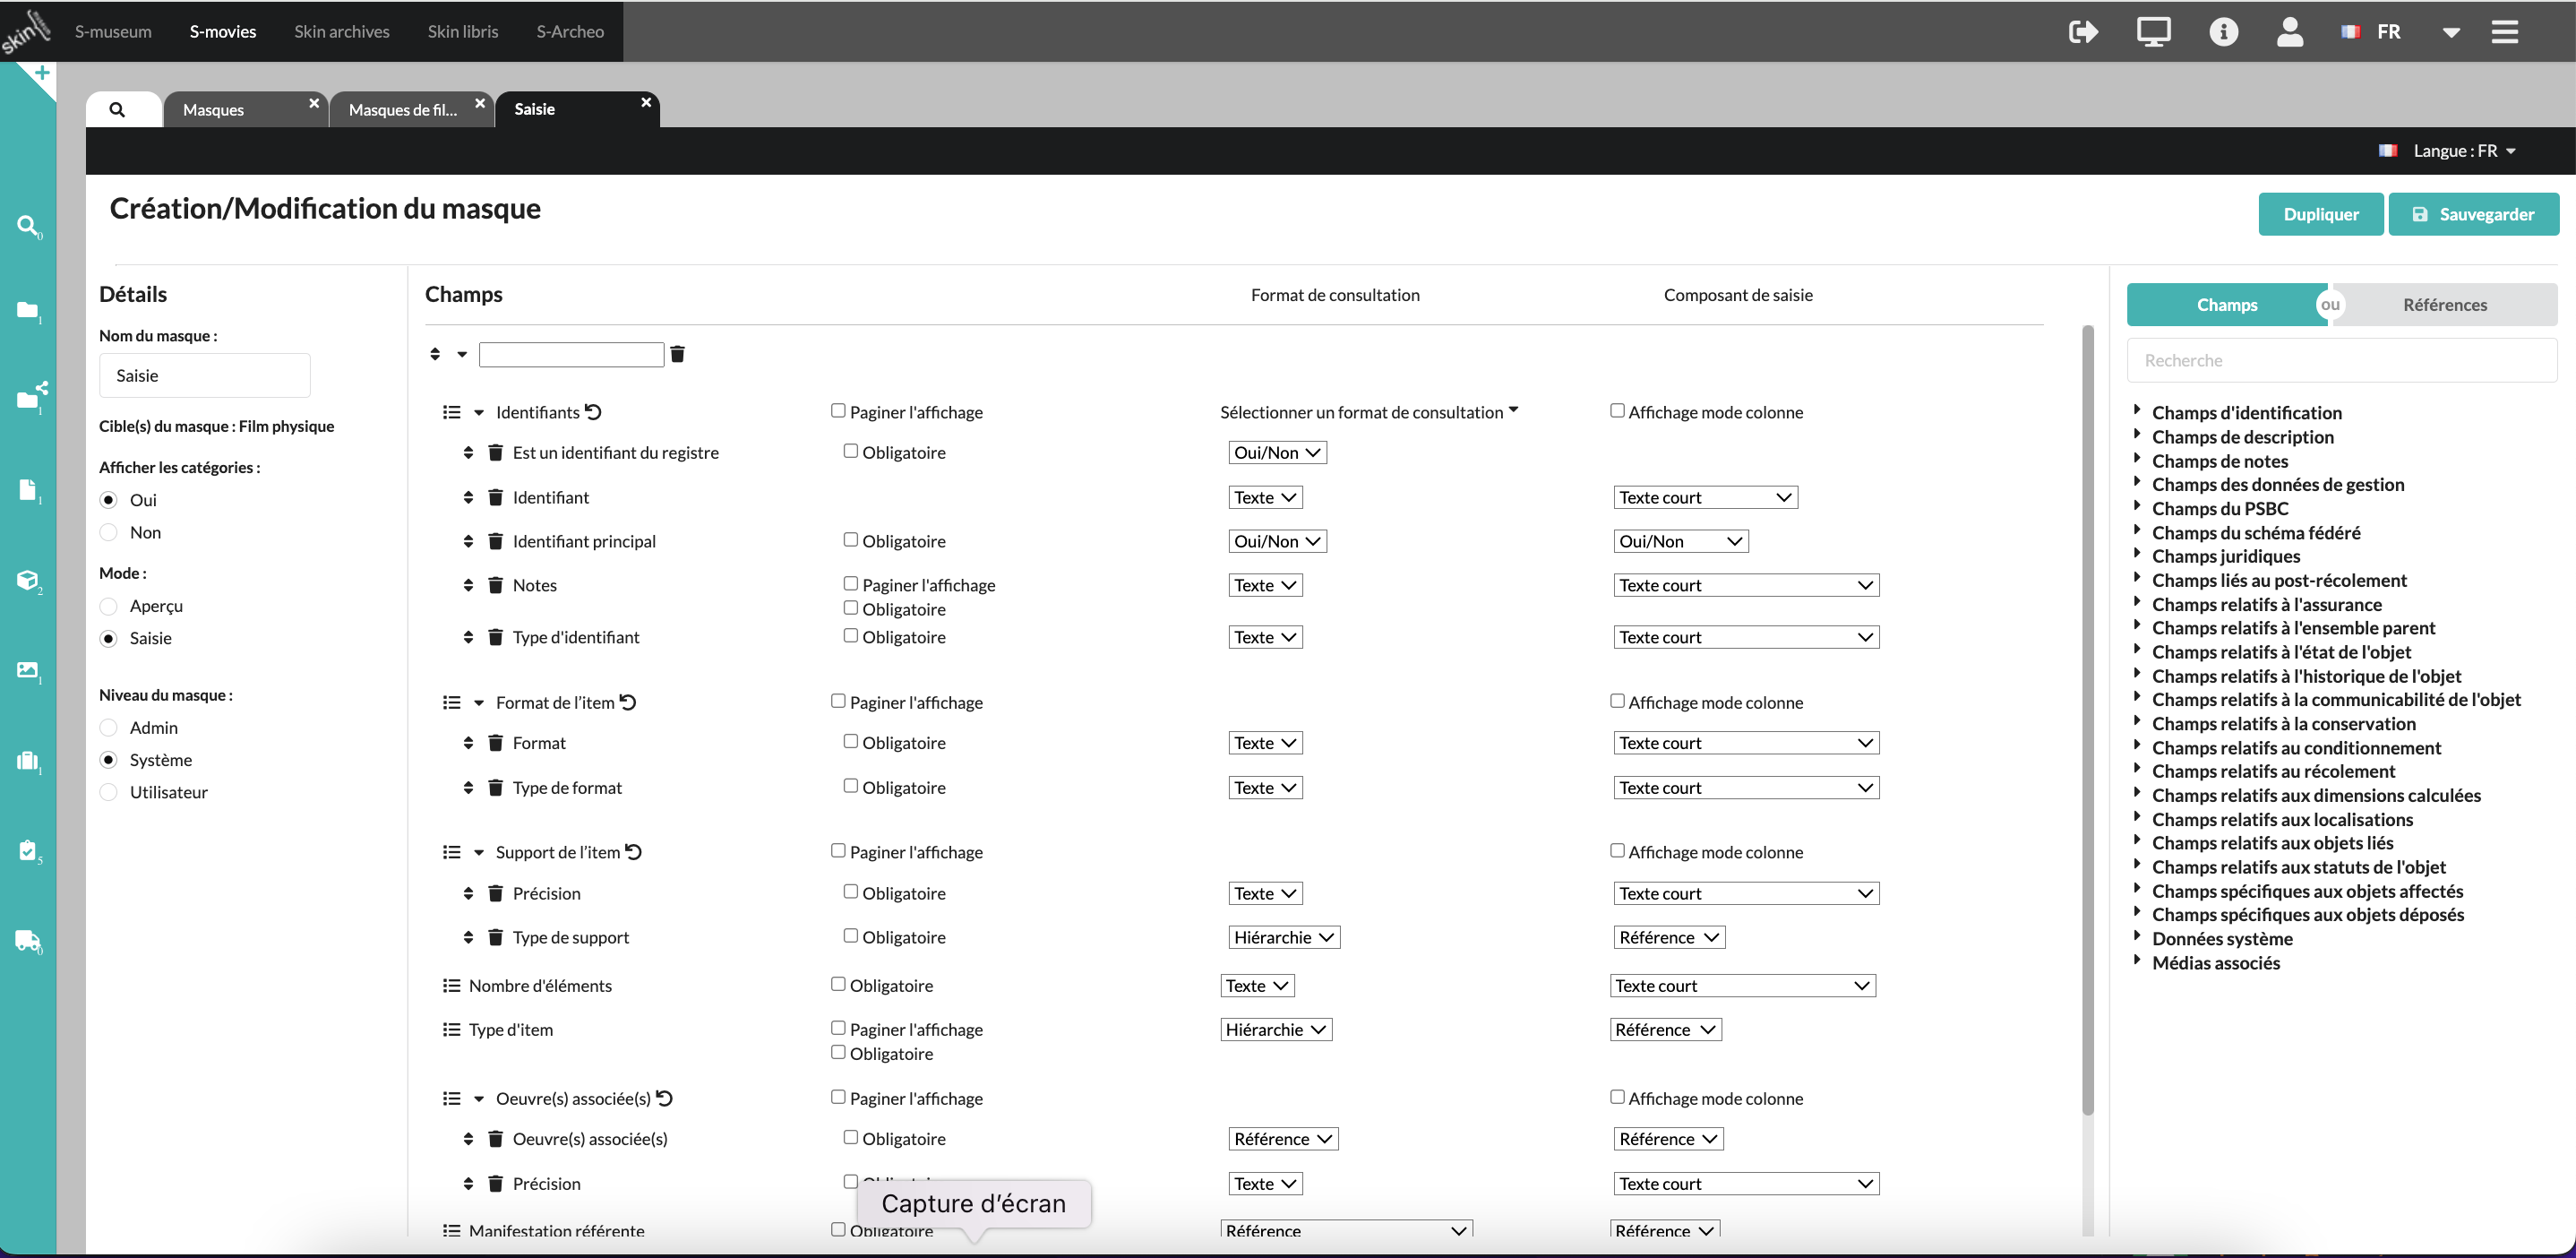
\includegraphics[width=1.0\textwidth]{images/image2.png} 
	
	\caption{Configuration des masques de saisie au niveau Item} 
	
	\label{figMasques} 
	
\end{figure}

Ce masque pourra ensuite être assemblé en tant qu’onglet au sein d’un menu d'une notice de film physique, permettant à l'utilisateur d'y remplir les champs que nous avons mentionnés. Ici, le menu d’une notice de film physique qui contient le masque de saisie mentionné plus haut :  

\begin{figure}[htbp] 
	
	\centering 
	
	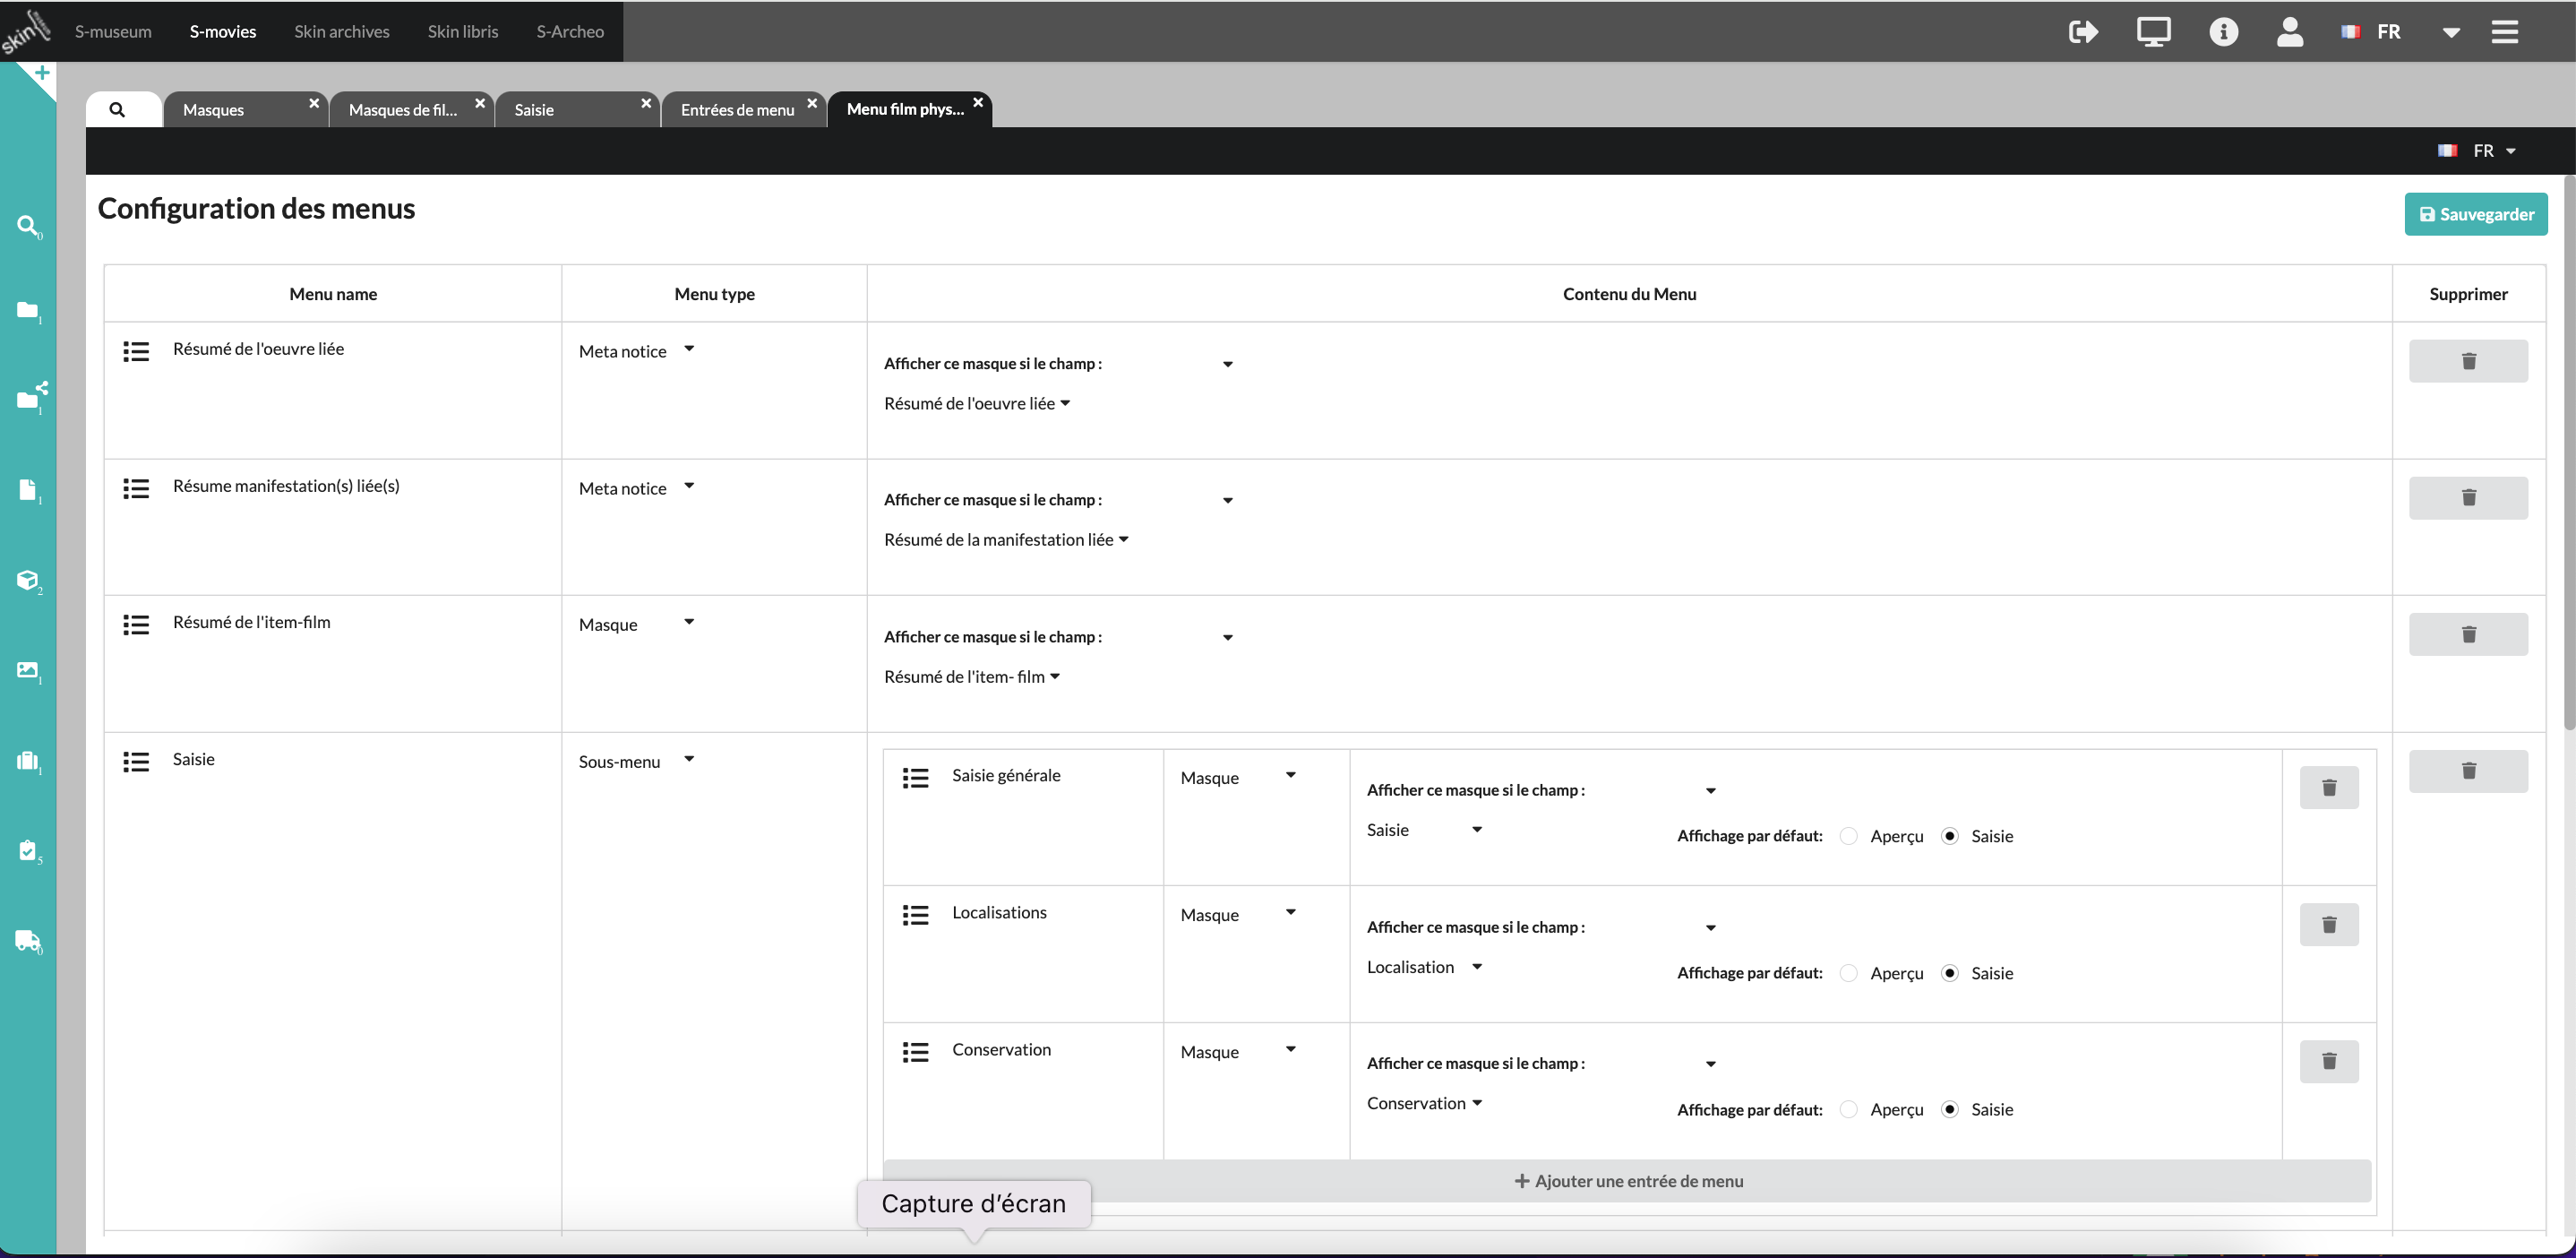
\includegraphics[width=1.0\textwidth]{images/image3.png} 
	
	\caption{Configuration du menu d'une notice de film physique} 
	
	\label{figMenuFilm} 
	
\end{figure}

Et ici la manière dont il s’affiche pour l’utilisateur, à la saisie dans une nouvelle notice de film physique :  

\begin{figure}[htbp] 
	
	\centering 
	
	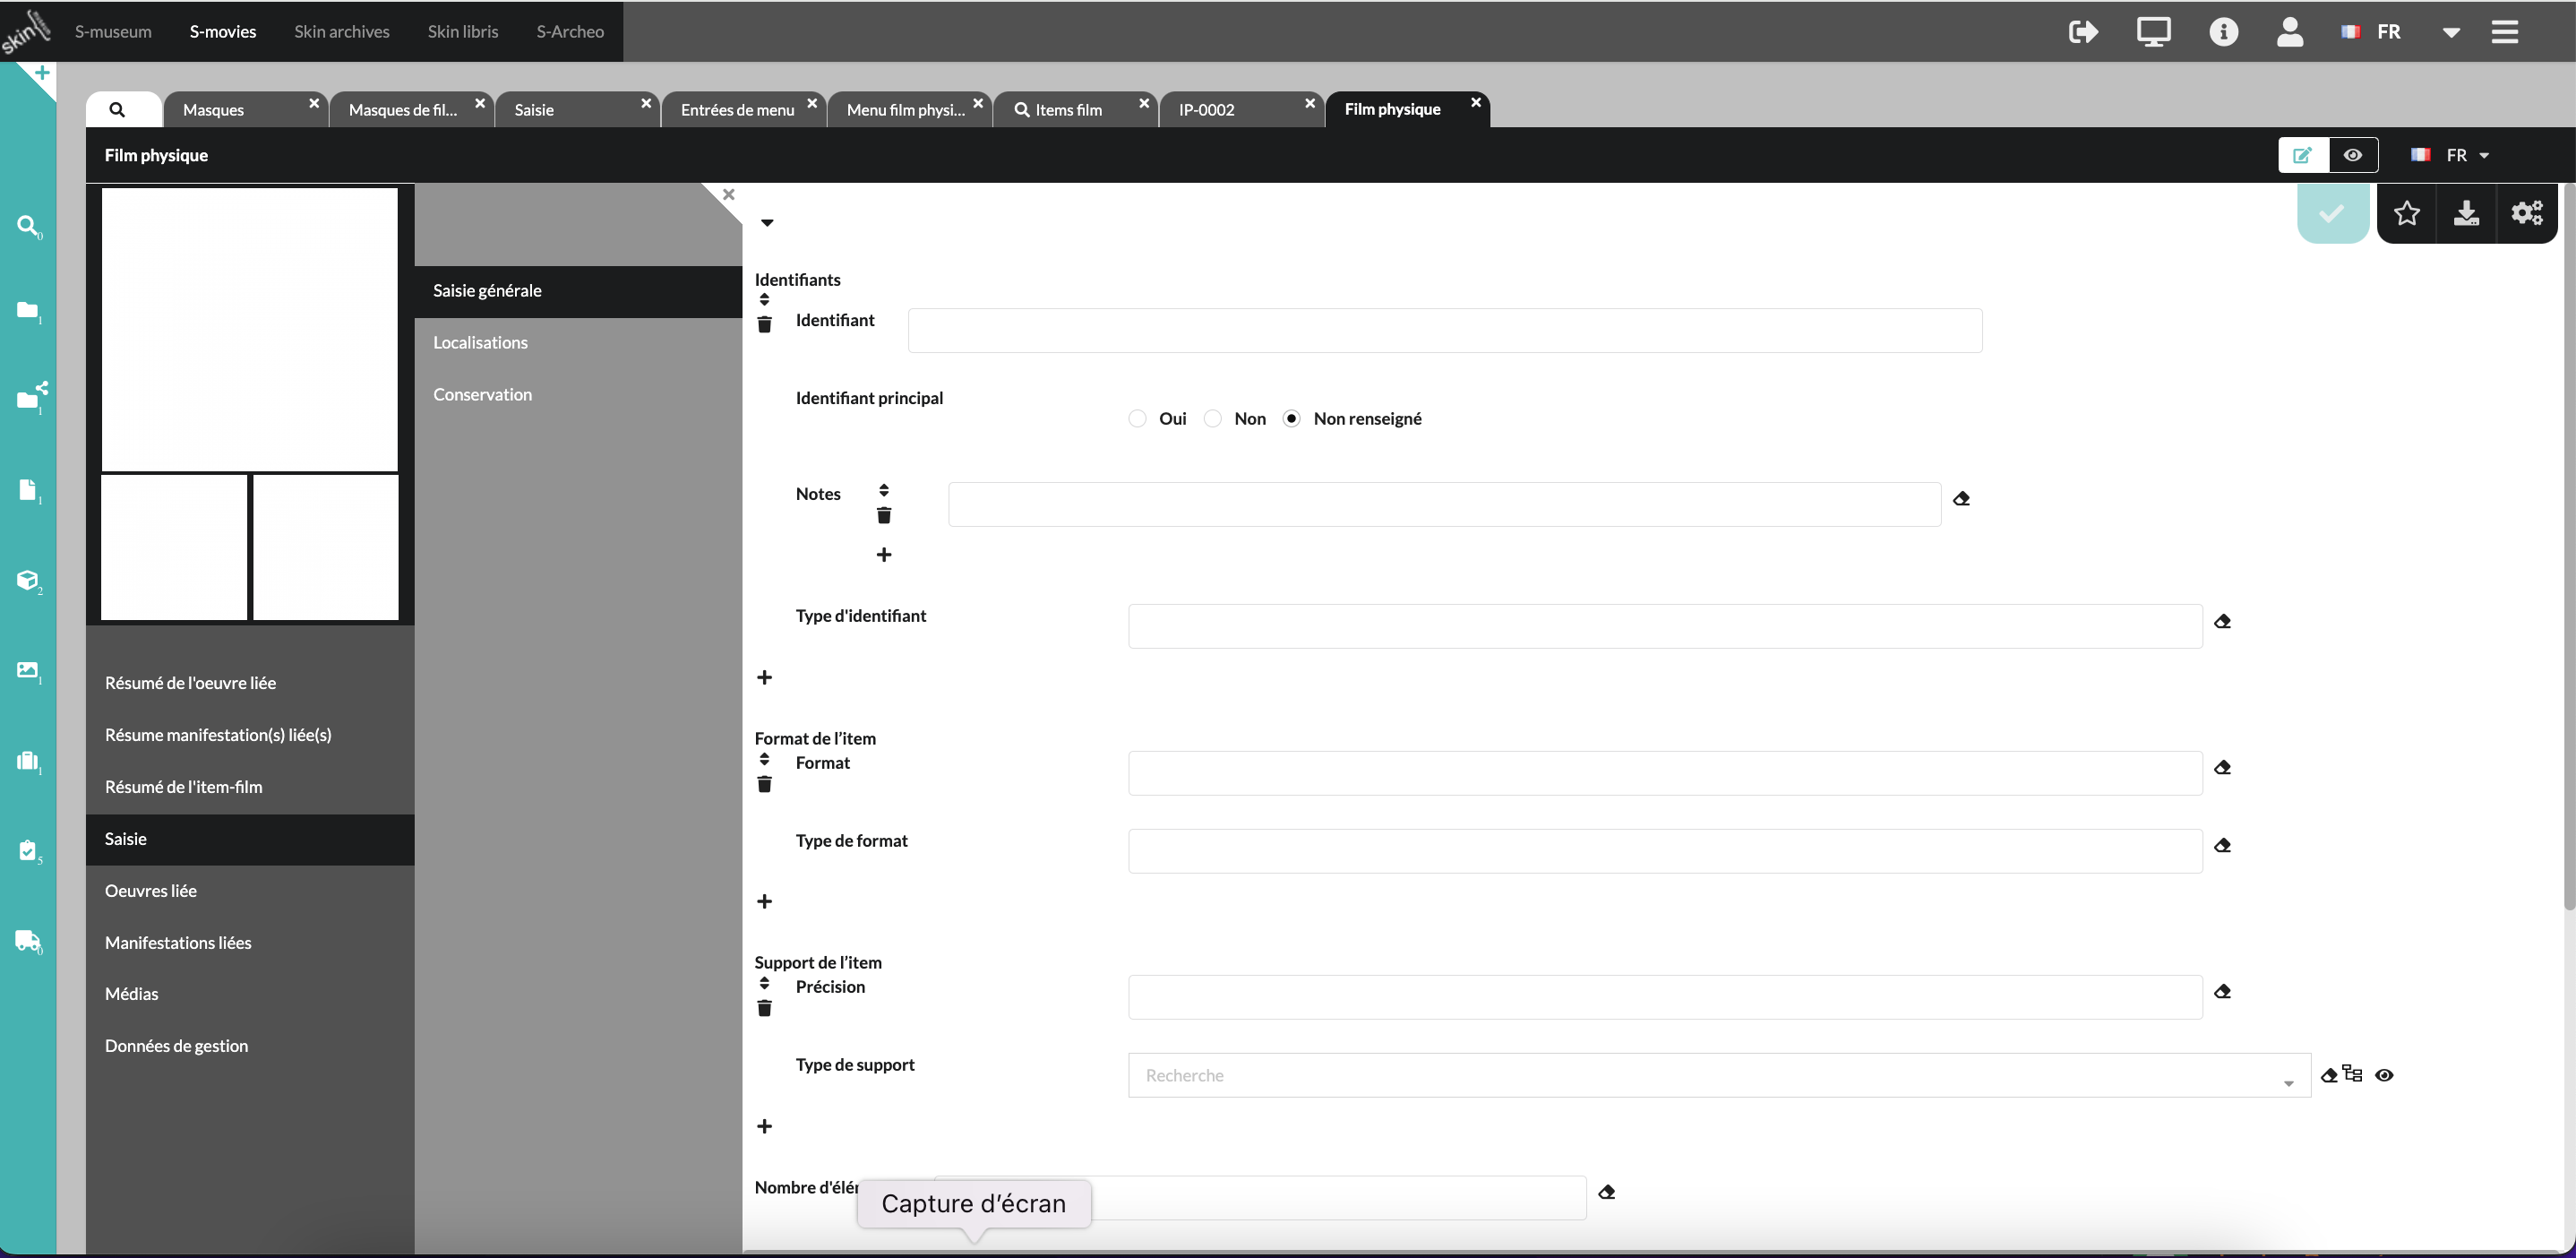
\includegraphics[width=1.0\textwidth]{images/image4.png} 
	
	\caption{Affichage du menu d'une notice de film physique à la saisie} 
	
	\label{figAffichageMenu} 
	
\end{figure}


Ce système d’organisation des masques de saisie au sein de menus permet également d’effectuer des liens avec d’autres types de notices et donc d’autres entités du FRBR. Par exemple la capture d'écran suivante \ref{figMenuGrilles}, montre que dans un menu de film physique, les onglets Œuvre liée et Manifestations liées permettent d’obtenir une grille de recherche, au sein d’une notice de film physique, affichant l’Oeuvre liée au film et les Manifestations dont il découle. 

\begin{figure}[htbp] 
	
	\centering 
	
	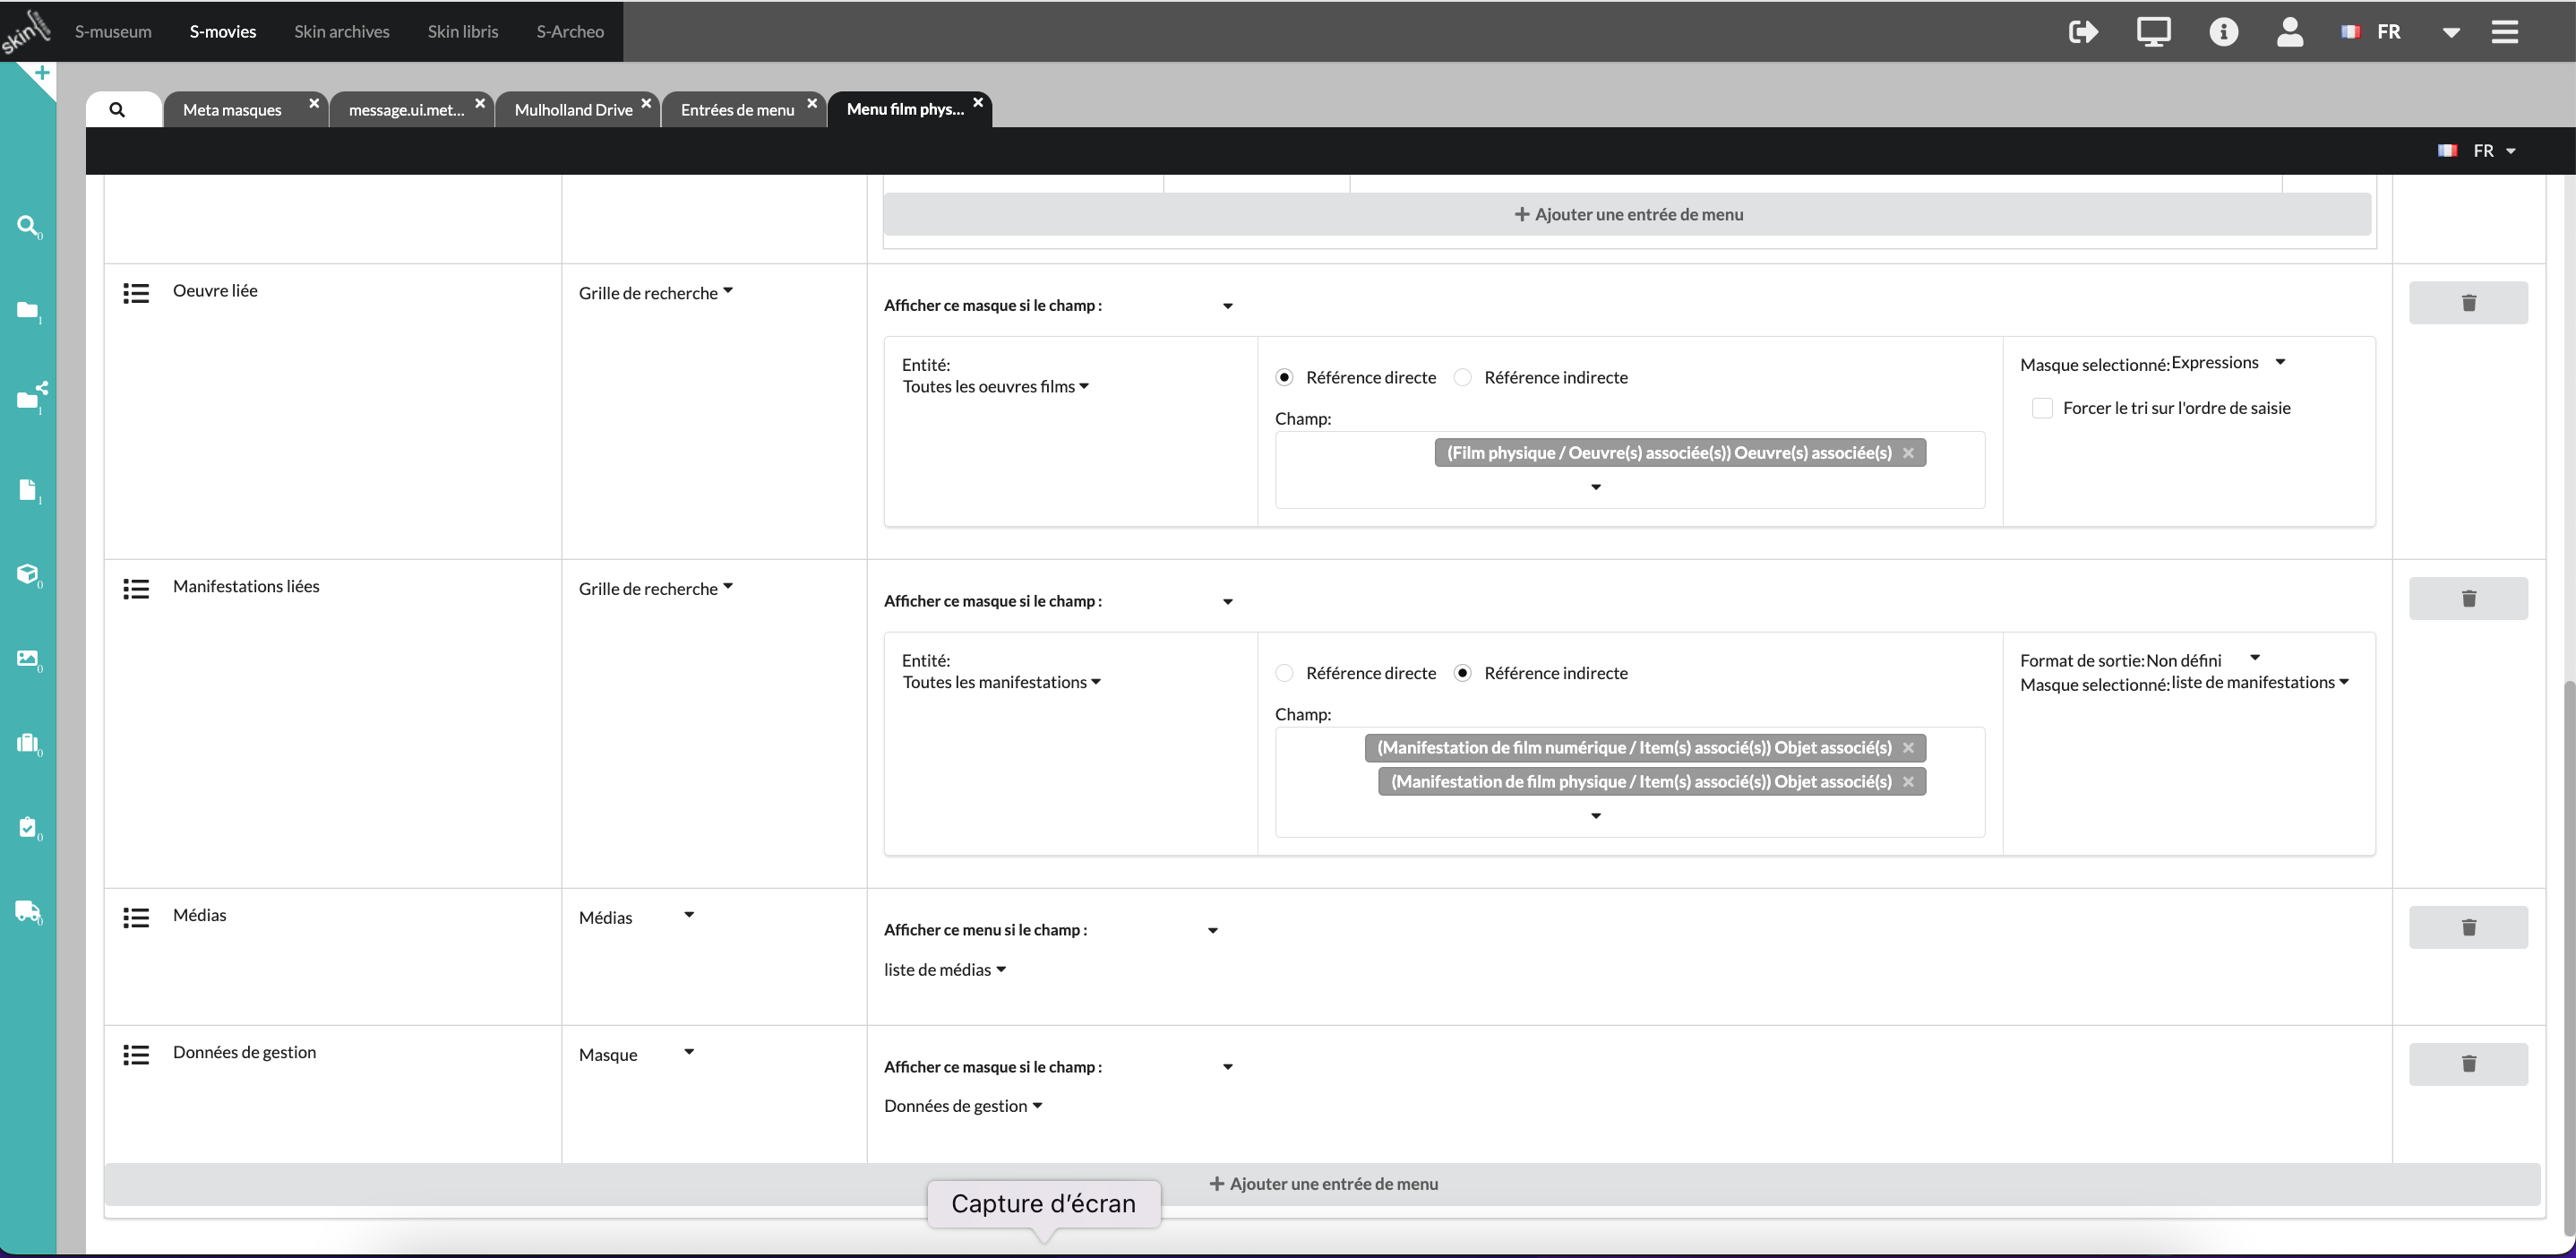
\includegraphics[width=1.0\textwidth]{images/image8.png} 
	
	\caption{Configuration de grilles de recherche pour l'affichage des éléments liés} 
	
	\label{figMenuGrilles} 
	
\end{figure}

L’affichage pour l’utilisateur au sein de la notice de film physique est le suivant, avec d’une part, l’Œuvre liée(\ref{figOeuvresLiées}, et d’autre part, les Manifestations liées \ref{figManifsLiées}: 

\begin{figure}[htbp] 
	
	\centering 
	
	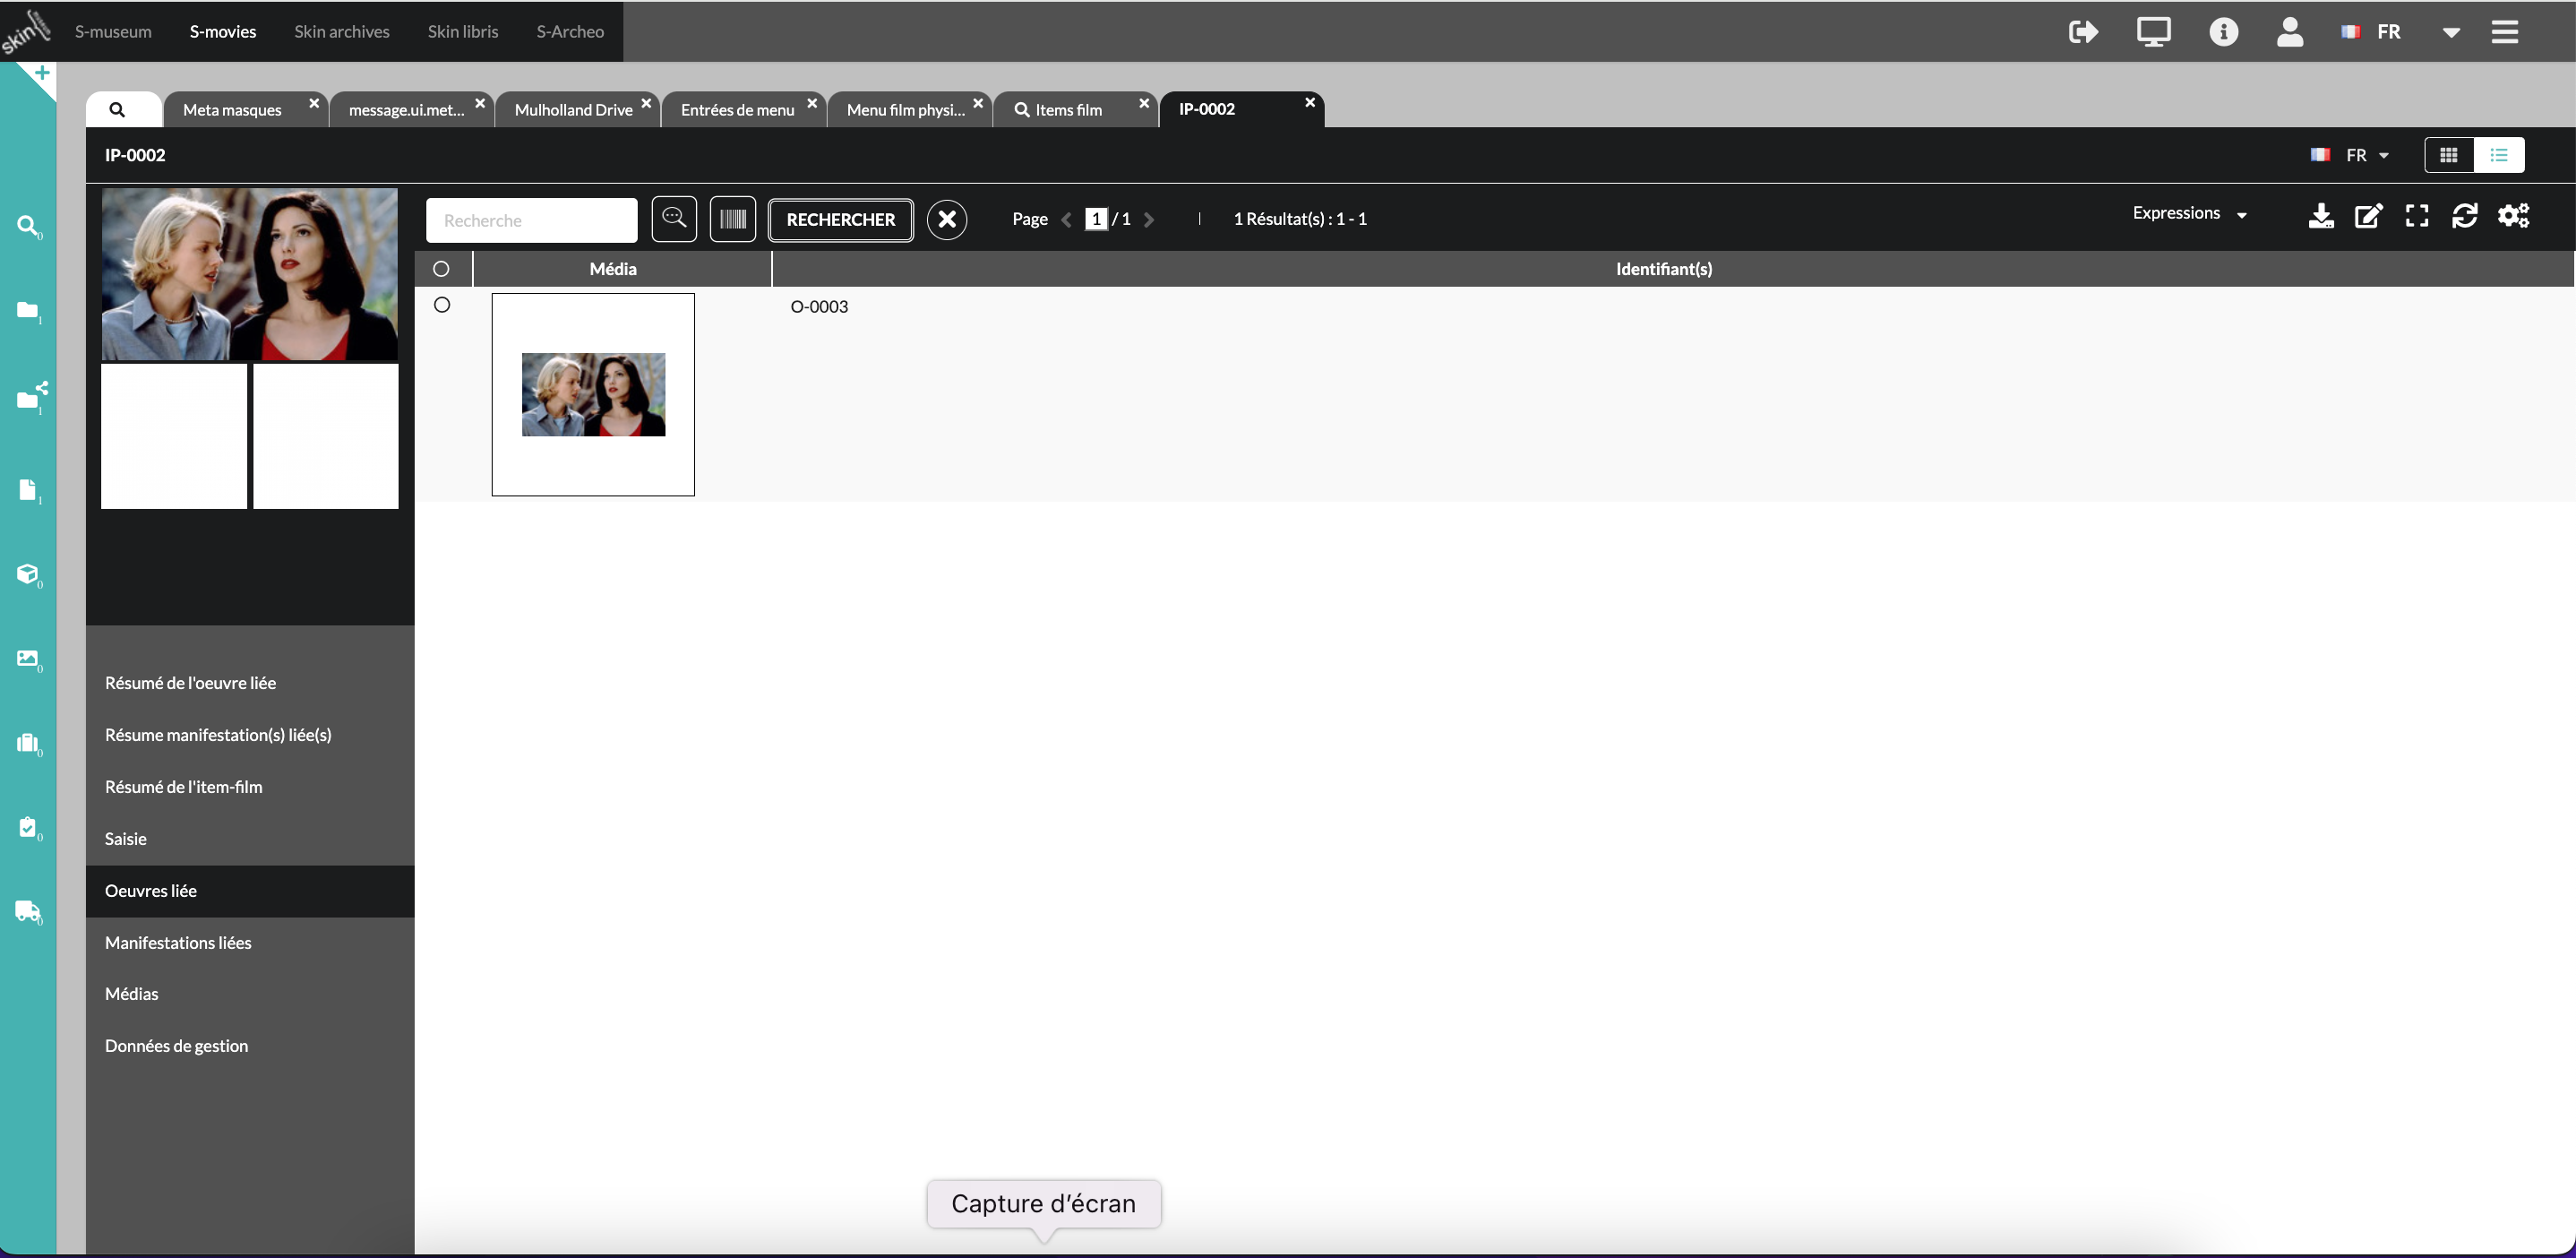
\includegraphics[width=1.0\textwidth]{images/image9.png} 
	
	\caption{Affichage des Oeuvres liées dans une notice d'item} 
	
	\label{figOeuvresLiées} 
	
\end{figure}

\begin{figure}[htbp] 
	
	\centering 
	
	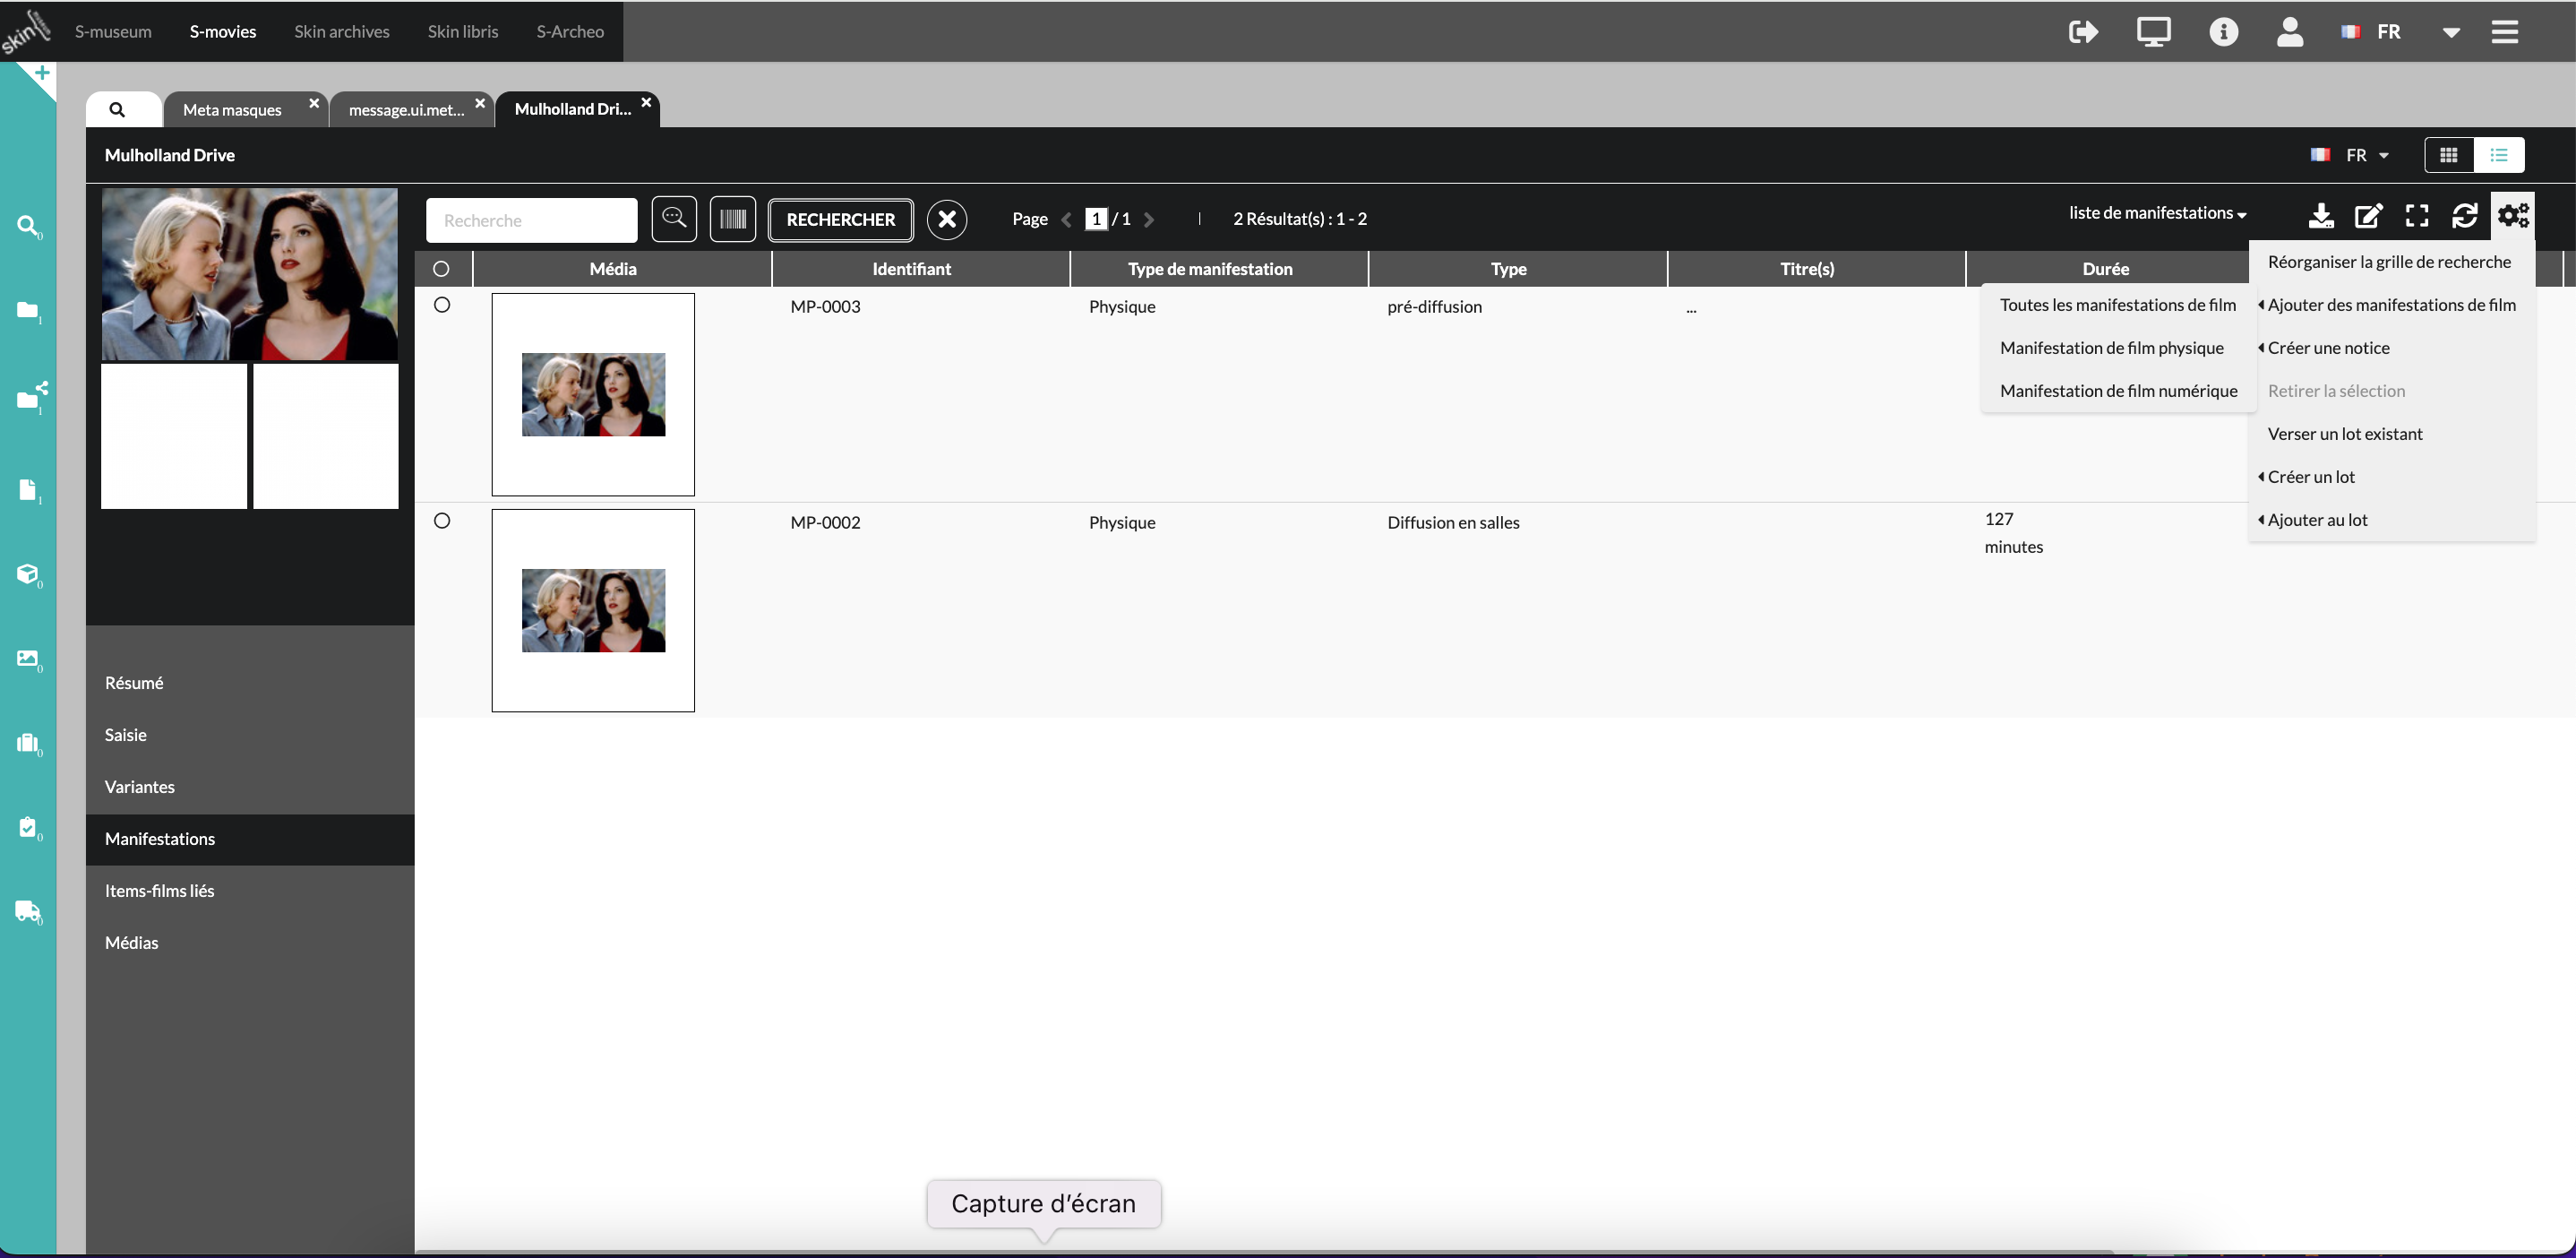
\includegraphics[width=1.0\textwidth]{images/image7.png} 
	
	\caption{Affichage des Manifestations liées dans une notice d'item} 
	
	\label{figManifsLiées} 
	
\end{figure}

Toutefois, les espaces de travail structurés sur le modèle FRBR, comme c'est le cas de S-Movies, requièrent un niveau de configuration supplémentaire, afin de concrétiser le découpage de la description en niveaux hiérarchiques. C'est le rôle des méta-masques, des formulaires de masques de saisie pouvant cibler les champs de plusieurs types de notices –et donc plusieurs niveaux du FRBR à la fois, afin d'imbriquer ces niveaux de description au sein d’une même notice. Ce système permet à l'utilisateur de saisir implicitement des éléments de description sur plusieurs niveaux du FRBR en une seule notice, permettant de surcroit au système de produire un héritage des champs d’un niveau à l’autre du FRBR.  

Concrètement, dans S-Movies, la notice d'Œuvre/Expression pointe sur les champs de l'Œuvre et de l'Expression, la notice de Manifestation pointe sur les champs de l'Œuvre, l'Expression et la Manifestation, la notice de l'Item pointe sur l'Œuvre, l'Expression, la Manifestation et l'Item. \textbf{(Faire un schéma explicatif) (citer le mode d'emploi interne ?)}. Ce mode de paramétrage de la description permet d’intégrer aux niveaux du FRBR inférieurs des champs hérités des niveaux supérieurs.  

\footnote{Notons que la présence du niveau Expression contredit le modèle FRBR préconisé par la FIAF, qui fusionne le niveau Expression dans celui d’Œuvre. Etant donné que Skinsoft possède d’autres espaces de travail modélisé sur le FRBR, comme c’est le cas de l’espace dédié à la gestion des collections bibliographiques, le niveau Expression existe seulement en théorie, mais inutilisé en pratique au sein de S-Movies.} 

Ici par exemple (\ref{figMetamasque}), un méta masque de saisie pour une notice de film physique, ciblé sur l’expression, le film physique, la manifestation de film physique, l’œuvre cinématographique : 

\begin{figure}[htbp] 
	
	\centering 
	
	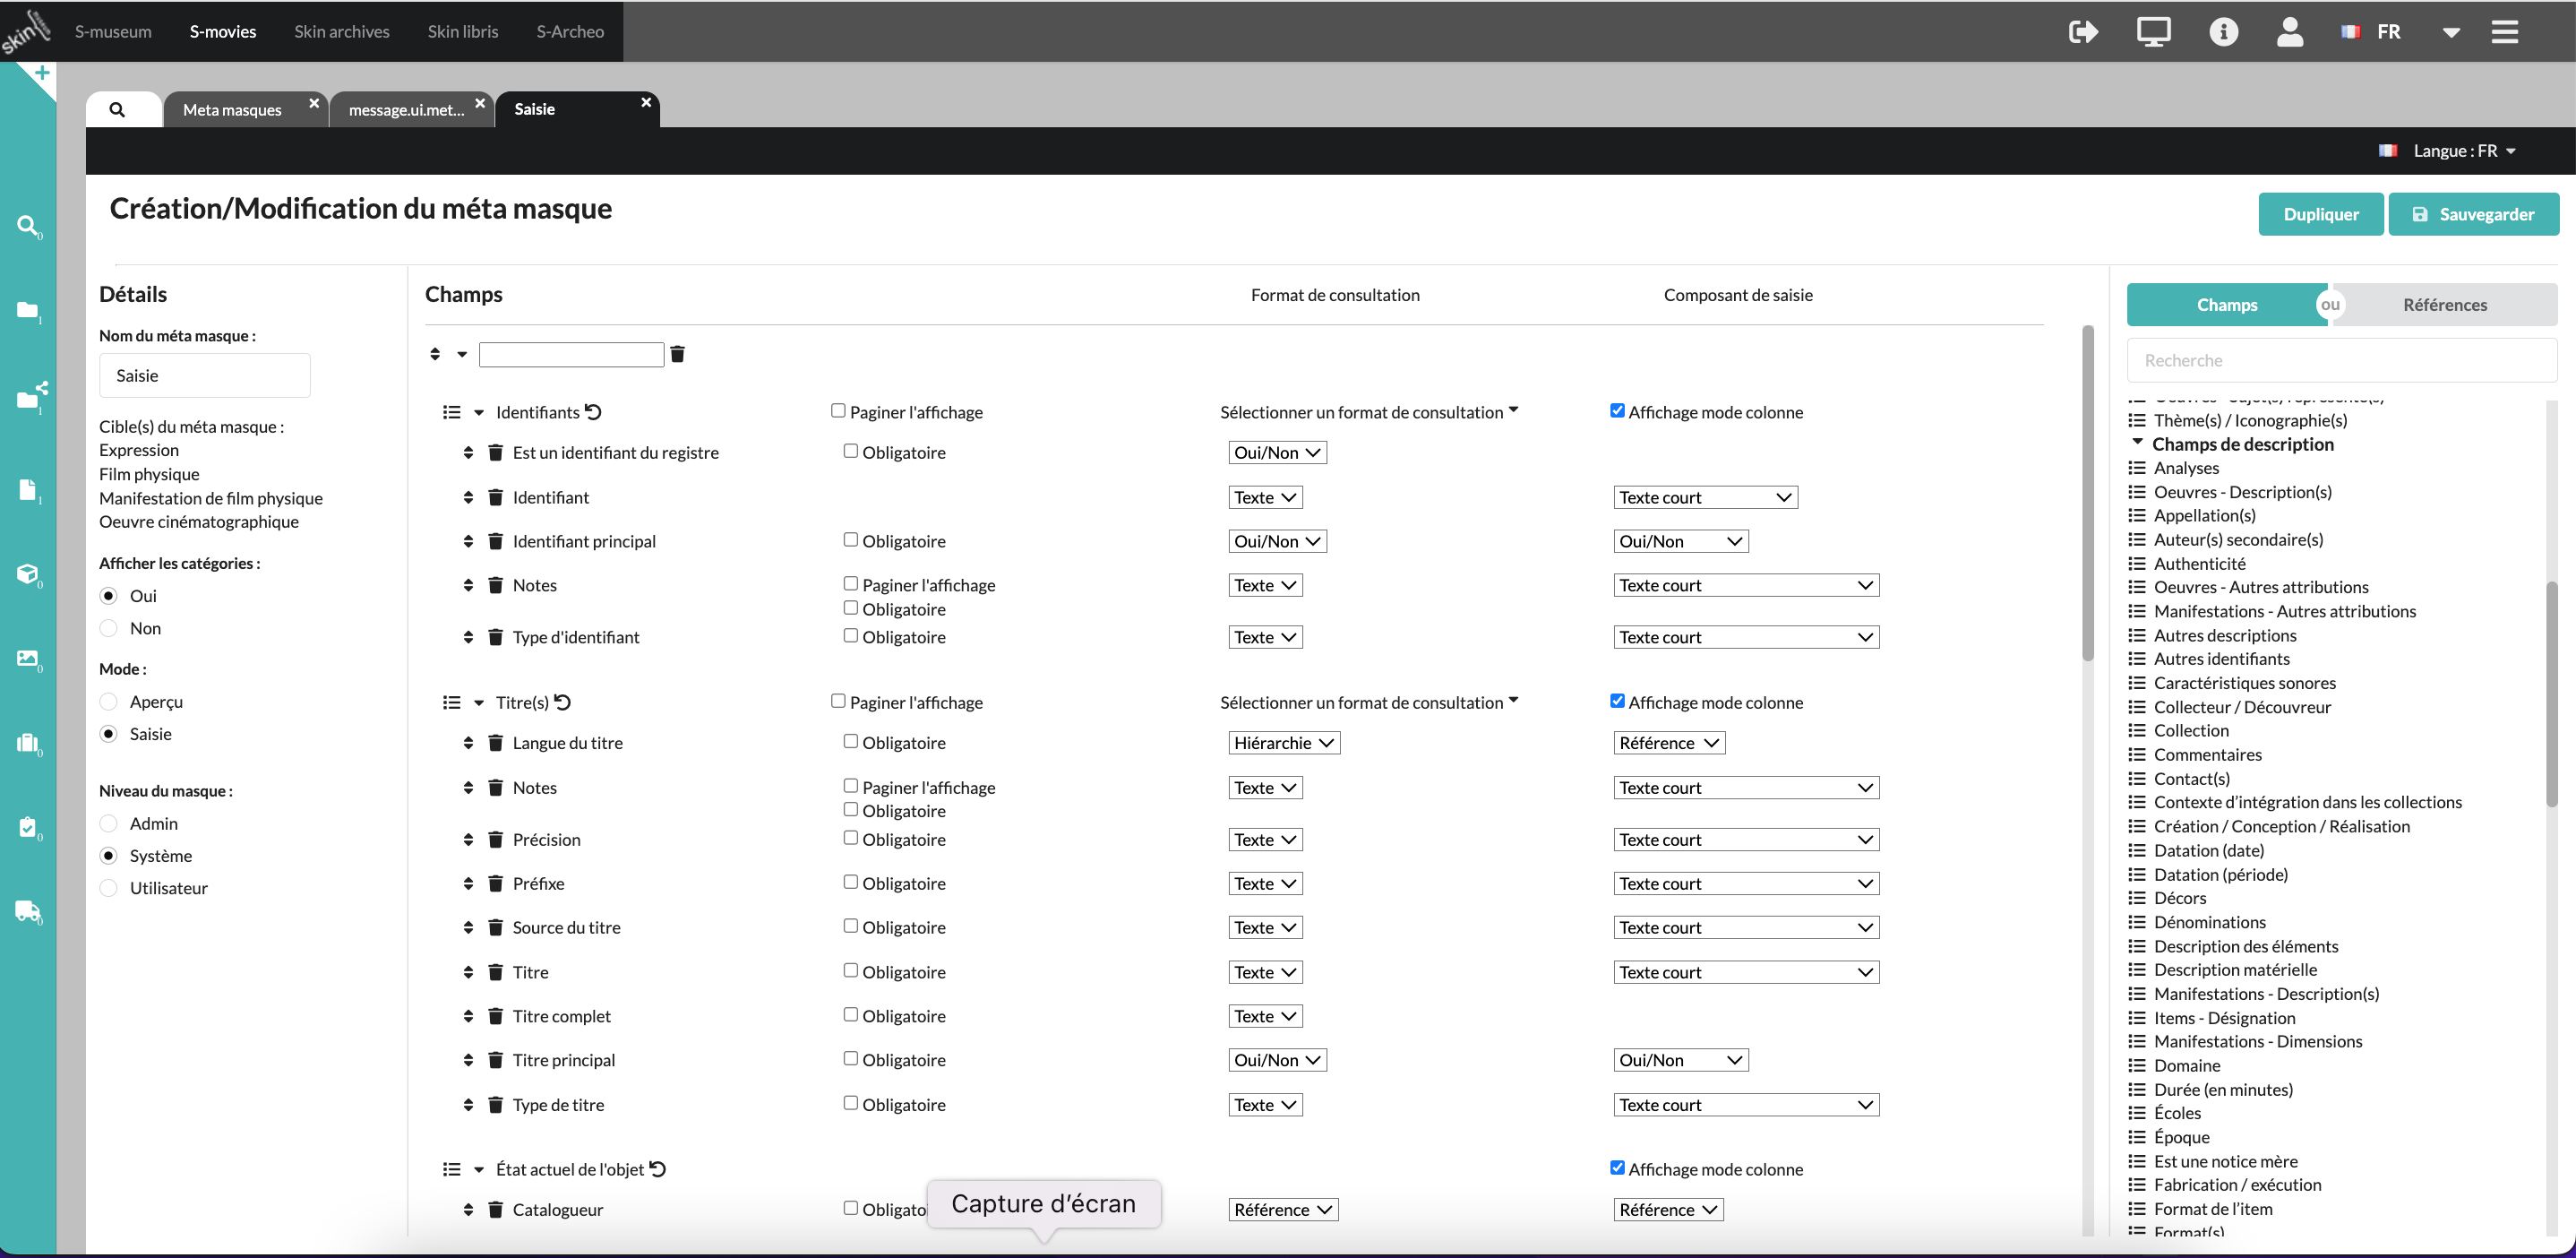
\includegraphics[width=1.0\textwidth]{images/imageb.png} 
	
	\caption{Configuration d'un méta-masque au niveau Item} 
	
	\label{figMetamasque} 
	
\end{figure}

À droite, les champs disponibles signalent à quel niveau de description ils appartiennent. Par exemple ci-dessus (\ref{figMetamasque}), le champ description appartient au niveau Œuvre, le champ dimensions appartient au niveau Manifestation.

%(: média (notice du fichier numérique, média), accessoire (modèle d'accessoire, accessoire), contenant (modèle de contenant, contenant).) 

Ces masques et méta masques créent ainsi une structure pérenne qui fait l'objet d'un paramétrage individuel qui permet d’ajuster la structure en fonction du type de collection et des usages métiers du client concerné. Ce paramétrage est défini au cours d’un travail de mapping entre les données client et la structure proposée par Skinsoft, afin de trouver un accord sur les champs qui seront utilisés pour la description des collections. L'équipe de Skinsoft organise ensuite ces champs dans des formulaires de saisie (masques et méta masques), eux-mêmes organisés pour constituer des menus de notice et des grilles de résultats de recherche. L'équipe produit également des imports de thésaurus propres aux usages de l'institution en question, afin d'assurer l'interopérabilité des données saisies. %Afin d'assurer l'interopérabilité des données, l'indexation des champs est liée à des thésaurus et des référentiels contrôlés qui ont importés au moment de la configuration de l'espace de travail pour le client. À développer  

Les fondements de l'architecture de S-Movies, doublement adaptée d’une part aux collections cinématographiques et d’autre part aux pratiques métiers spécifiques à chaque institution, constitue la condition de la qualité des données et de l’expérience utilisateur. L'enjeu de l'espace de travail est d'offrir une interface qui permette à l'utilisateur de décrire les collections en plusieurs niveaux sans difficulté et de pouvoir circuler entre ces niveaux et les liens qu’ils entretiennent. Cette circulation est notamment permise par les grilles de recherche que nous avons évoquées dont le paramétrage permet d’afficher les entités liées pour chaque notice. De plus, les différents outils de recherche permettent de circuler au sein des éléments de description indexés. (À développer ?) 

Toutefois, malgré la haute configurabilité de l’interface, l’hétérogénéité des corpus audiovisuels gérés d’une institution à l’autre complexifie le travail de mapping qui doit être effectué. En effet, la modélisation FRBR préconisée par la FIAF est un cadre qu’il s’agit d’ajuster aux pratiques spécifiques de gestion des collections, elles-mêmes adaptées au type de corpus géré. L’ajustement à des corpus audiovisuels spécifiques complexifie potentiellement la fluidité de la navigation entre les liens des différentes entités du FRBR au sein de l’interface.   

%Présentation espace S-Movies : aperçu des fonctionnalités communes et spécifiques (à placer en annexe ?): ces fonctionnalités sont chacune rattachées à un ou plusieurs niveaux du FRBR 

%- gestion des entrées : création d'un objet de collection via l'import de son média 

%- gestion des médias : associer un nouveau média à une notice de film ou un média existant 

%définir des vignettes sur les notices de films à l'aide des médias importés  

%- documents associés  

%- table collections/thématiques : regroupement des collections par thématiques : décrit le contexte de la collection, de l'assemblage des films, et présentent les items présents dans cette collection 

%- projets et mouvements : intervention, conservation, acquisitions, entrées, expositions, prêts, diffusion/programmation 

%fonctionnalités communes : gestion des contrats, évènements, interventions, expositions 

%Lien de la FIAF à S-Movies : mise en application du manuel de la FIAF, remodélisation, adaptable selon les corpus. tension public/privé 



%à bouger dans la première sous partie 

%S- Movies s'appuie sur deux normes descriptives audiovisuelles européennes : la norme EN 15744, qui définit le contenu obligatoire de description pour l'identification d'un film, ainsi que la norme EN 15907 qui découle du manuel de la FIAF et décrit une structure en couches et niveaux de données. Ces normes définissent les métadonnées essentielles pour faciliter l'échange de données et l'identification des films. \footcite{zotero-item-646} 



%Au niveau de la description des archives, il s'appuie sur la norme RDA pour la description et l'accès aux ressources. \footcite{zotero-item-646} 

%mentionner les données techniques ? : type de serveur, type de base de données 
\section{\label{I_2_B}L'inscription des corpus de données dans la remodélisation du FRBR} 

En effet, la nature du corpus audiovisuel complexifie le paramétrage puisqu'elle conditionne la capacité des données à s'adapter et s'intégrer au sein du modèle FRBR. Le modèle FRBR fait partie d'une structure fixe de l'espace de travail, avec cette séparation en trois tables de saisie (Œuvres, Manifestations, Films), dont le paramétrage peut toutefois amoindrir la rigidité. Afin d'analyser la mesure dans laquelle les corpus s'intègrent au sein du modèle FRBR, nous analyserons dans cette sous partie deux corpus de données différents gérés au sein de l’application Skinsoft. \footnote{Notons que pour des raisons de confidentialité, nous décrirons les corpus de ces institutions sans les nommer de manière explicite.}.  

Premièrement, analysons l'intégration d'un corpus de cinéma dit "classique", au sein de l'espace de travail S-Movies. Cette collection est gérée par une institution qui préserve essentiellement des films de fiction issus d'une production commerciale "grand public" depuis les débuts du cinéma jusqu'à nos jours. Cette collection est composée d’œuvres cinématographiques à proprement parlé, dont la description prend tout son sens au sein d’une modélisation selon le FRBR. La production cinématographique étant une production industrielle, les films qui en sont issus s'adaptent particulièrement bien à un modèle de données par niveaux, ces différents niveaux correspondant aux étapes de production. Ces films, après leur création, ont donc été produits et distribué à une échelle plus ou moins large. Ainsi, dans ce cas précis, le modèle FRBR est plutôt bien adapté. La réalisation du film par le montage et le tournage est décrite au niveau Œuvre, ses versions sont décrites au niveau variante, son édition et sa distribution sont décrites au niveau Manifestation, et l'exemplaire individuel du film, conservé par l'institution est décrit au niveau Item. De fait, le paramétrage décrit dans le chapitre précédent peut être réalisé sans trop de complexité au sein du cadre modélisé par le FRBR de la FIAF. (Développer + ?) 

Deuxièmement, analysons l'implémentation d'un corpus plus spécifique, celui d'une collection de \textit{rushes} documentaires muets et non montés, tournées des années 1910 à 1920. Les \textit{rushes} en termes cinématographiques correspondent à des épreuves de tournages non montées\footcite{universalis.} Ces \textit{rushes} bruts, ont été tourné dans une optique de documentation sur différents sujets, et ne sont pas destinés à une diffusion auprès du grand public. 

Dans ce cas, l'absence de montage et de distribution commerciale rend difficile l'adaptation du corpus à la modélisation prévue par la FIAF, qui structure S-Movies. Si le contexte de création du tournage peut être décrit au niveau Œuvre, les niveaux de description inférieurs sont inadaptés. En effet, en l'absence de montage, la Variante n'existe pas puisque chaque \textit{rushe} correspond à une matière brute et unique. Ainsi, l'absence de différentes versions d'une même œuvre invalide l'entité de Variante.  

De la même façon, le niveau Manifestation perd de sa pertinence descriptive puisque ces \textit{rushes} ne sont ni produits ni distribué officiellement auprès d'un public. L'inscription de l'œuvre sur un support s'effectue ici de manière unique, et en un seul et même exemplaire. Les caractéristiques matérielles pourraient donc être décrites directement au niveau de l'item.  Ainsi, d'un modèle à quatre niveaux, il ne reste, dans ce cas précis, plus que deux niveaux de descriptions exploitables : l’Œuvre et l’Item. Toutefois, notamment pour des raisons de conservation, une œuvre peut être copiée sur différents supports, physiques ou numériques. En effet, l'institution peut être amenée à produire des copies d’une œuvre sur des supports plus stables à des fins de préservation ou de diffusion en ligne, par exemple. Ces différentes matérialisations, bien qu'elles ne soient pas issues d'un processus commercial de distribution, peuvent être décrites comme des Manifestations. Telle que définie par le manuel de la FIAF, une manifestation induit en effet, "tous les médias analogiques, numériques et en ligne associés à une matérialisation particulière d'une Œuvre/Variante." \footcite{zotero-item-646}. Sa description peut alors être justifiée par des objectifs de conservation : copie, numérisation, restauration. Selon le FIAF, la description d'une Manifestation inclut les attributs suivants, -ici sélectionnés selon leur niveau de pertinence pour un tel corpus : type de manifestation, format (incluant les champs suivants : type de support, caractéristiques sonores, caractéristiques de couleur), notes.  

Or, si théoriquement le niveau Manifestation peut être décrit, en pratique dans le cas de la description de ce corpus produite par l’institution, il ne l’est pas. Est-ce que le modèle de description utilisé en pratique correspond au modèle à deux niveaux présentés brièvement par la FIAF ?  

Si au sein d'une notice d'œuvre, les champs suivants sont décrits : identification, titre, créateur, description (sujet de la prise de vue), mots clés, films associés, manifestations associées, matériel non-film associé, archives associées, bibliographie, médias, données de gestion ; la table Manifestations, en revanche, contient un nombre conséquent de notices vides. En effet, l'application Skinsoft crée automatiquement une notice de manifestation liée lorsque l'utilisateur crée une notice d'item. Dans ce cas, l’entité Manifestation devient une condition structurelle afin de maintenir la cohérence du modèle, mais perd son sens au sein d’un contexte d'indexation concret. La table des items, quant à elle, est répartie en trois catégories d'objets : bobines, cassettes ---qui constituent les films physiques--- et films numériques. Lorsqu'un même film physique est présent en plusieurs exemplaires dans la collection, les notices sont distinguées par la mention "bobine originale" et "reproduction". Les notices de films physiques contiennent une description matérielle sur le support et la condition de ce support. Elles mentionnent également les collections liées vers d'autres Items et Œuvres, vers des médias et des documents. La manifestation référente est tout de même mentionnée mais il s'agit, nous l'avons évoqué, d'une notice factice. Enfin, les films numériques décrivent le support original depuis lequel la numérisation a été effectuée, les raisons de la numérisation ---par exemple, copie de sauvegarde---, et l'item physique qui a fait l'objet de cette numérisation.  

Par ailleurs, un élément précis a retenu notre attention dans le cadre de notre étude. En effet, la présence de \textit{time-codes} ---marqueurs temporels dans des notices de films numériques, traduisant l'inscription de la copie numérisée dans une œuvre plus large. En effet, certaines Œuvres-rushes, dont les modalités matérielles sont décrites dans une notice de film physique, ont été divisées en extraits puis numérisées. Étant donné que les Œuvres conservées sont des rushes non montés, cette division en extraits a pour but de réaliser une forme de montage et de rendre ces films intelligibles via une diffusion en ligne. Ainsi, la plupart des films numériques gérés au sein de S-Movies sont issus de ce découpage depuis les rushes originaux. Les repères temporels expriment le rattachement précis de l'item numérique au sein d'un item physique.  

Ainsi, la modélisation de données adaptées à ce corpus audiovisuel précis s'apparente à un modèle hiérarchique à deux niveaux, celui d'une Œuvre matérialisée dans une Manifestation/Item, fusionnés en une seule entité. Cette hiérarchie à deux niveaux est brièvement décrite dans le catalogue de la FIAF en tant qu'exemple, mais ses modalités ne sont pas détaillées. (À développer?) 

\begin{figure}[htbp] 
	
	\centering 
	
	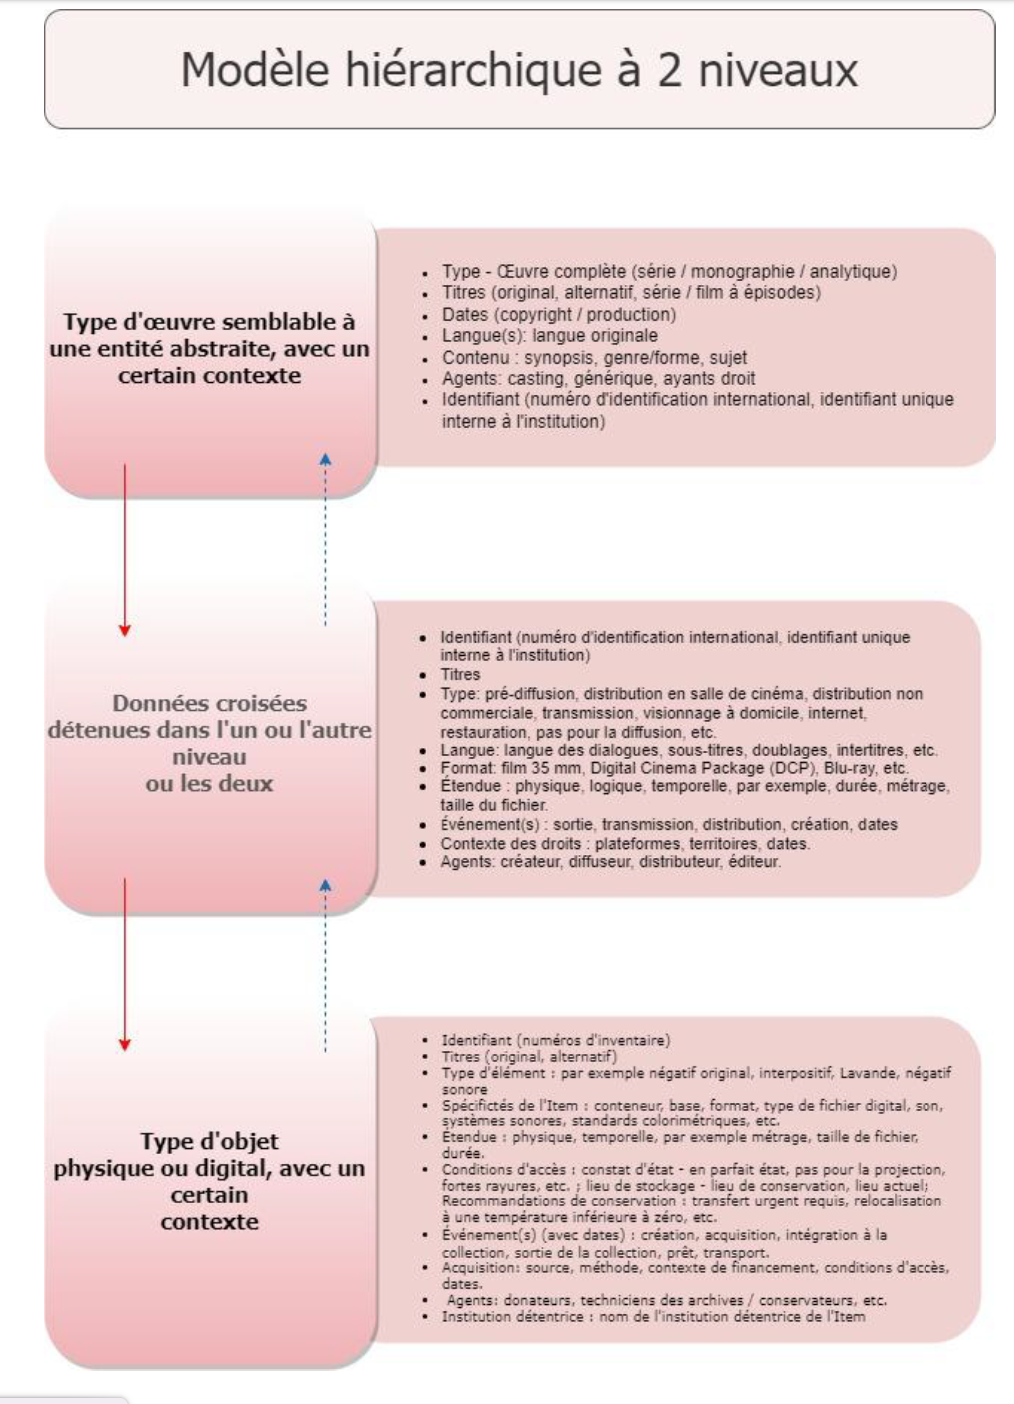
\includegraphics[width=1.0\textwidth]{images/imagec.png} 
	
	\caption{Modèle hiérarchique à deux niveaux schématisé par le manuel de la FIAF} 
	
	\label{figModele2Niveaux} 
	
\end{figure}

Développer davantage le schéma de données que ça produit dans l’appli client ? Avec un schéma ? À partir des captures d’écran suivantes : schématiser les liens complexes entre éléments pour le corpus en question  

Par exemple : Une notice Œuvre est liée à un item numérique, lui- même lié à un ou plusieurs films physiques : cassette, bobine, avec le time code mentionné pour traduire la place de l’extrait/film numérique au sein de ces supports physiques.  

Les films physiques : contiennent la liste des films numériques qu’ils ont pour extrait + les différentes reproductions du film physiques sur d’autres supports physiques : plusieurs bobines, plusieurs cassettes (à des fins de conservation)  

Si l'espace de travail S-Movies parvient à maintenir le modèle du FRBR en trois niveaux principaux pour les corpus audiovisuels standards, la description de corpus plus spécifiques éclipse notamment le niveau Manifestation pour ne conserver qu'une hiérarchie à deux niveaux. L’analyse de l’inscription d’un corpus donné au sein de la modélisation de données proposée par S-Movies soulève des interrogations sur la fluidité de la navigation de l’utilisateur au sein de l’interface.  En effet, le caractère brut du corpus observé nécessite une description fine du contenu afin de restituer une intelligibilité, d’habitude produite par le montage, qui doit être prévue par une saisie ergonomique au sein de l’interface. Afin d’adapter l’espace de travail à des corpus aussi spécifiques, l’éditeur Skinsoft engage notamment une démarche de refonte de S-Movies, dont l’objectif est de repenser d’une part l’interface fondée sur le FRBR, et d’autre part d’intégrer des fonctionnalités innovantes d’indexation automatique afin d’assister l’utilisateur dans la description des collections. C’est dans ce contexte d’innovation technique que s’inscrit notre stage, au cours duquel nous avons étudié l’usage de S-Movies afin d'en améliorer l’expérience utilisateur, et ainsi préparer l’implémentation de fonctionnalités automatiques pour la description des collections audiovisuelles. 
\section{\label{I_2_C}Vers une refonte de S-Movies} 

Si le cadre posé par la modélisation FRBR s’avère limité pour des collections spécifiques telles que celles que nous avons analysé, le modèle induit des difficultés plus globales au niveau de l’interface et de la navigation utilisateur. Le FRBR est fondé sur des besoins utilisateurs dont l’objectif serait “d’identifier, sélectionner et acquérir” efficacement l’ensemble des éléments décrits et répartis entre différents nie=veaux hiérarchiues \footcite{zotero-item-646}. Ces besoins semblent respectés au sein de l’interface S-Movies, via la navigation permise entre les entités et les outils de recherche disponibles. Toutefois, une double complexité subsiste dans l’implémentation de la modélisation FRBR au sein d’une interface. D’une part, il reste complexe de mettre en place une interface intuitive permettant à l’utilisateur de connaître immédiatement le rôle descriptif de telle entité du FRBR et sa place au sein de la hiérarchie du modèle. D’autre part, la visualisation des liens entre les entités du FRBR reste limitée, puisqu’elle supposerait des développements supplémentaires innovants tels que la visualisation en graphe, par exemple.  

Parmi les complexités d’interface révélés par l'expérience utilisateur, certains éléments semblent anodins. Par exemple, l’affichage d’une hiérarchie inversée du FRBR dans le menu de l’application, pouvant nuire à l’intuitivité du rôle de chaque entité pour la description des collections. En effet, au sein du menu, les tables sont présentées de telle manière à ce que le plus bas niveau du FRBR (l'item) apparaisse en haut, suivi de la manifestation et du plus haut niveau (l'œuvre). Cet affichage visuel descendant peut induire en erreur l'utilisateur sur la navigation hiérarchique à employer au sein du modèle. De plus, au sein de S-Movies le plus bas niveau de la hiérarchie (l’Item) est désigné par la notion de “Film”. Or, dans un contexte cinématographique, le film peut communément désigner à la fois une œuvre et un item individuel. La notion de film n'évoque pas le caractère unique et individuel de l'exemplaire tel qu'il est défini par le manuel de la FIAF. Une autre confusion terminologique potentielle peut être créée par la présence de la notion d'Expression, alors même que ce niveau, issu du modèle FRBR bibliographique, est fusionné dans celui d'œuvre.  

La visualisation des liens entre les entités descriptives au sein de l’interface est également motrice d’améliorations au sein de l’espace de travail. L'interface actuelle permet, après configuration, de visualiser les liens d’une notice avec d’autres notices issues de niveaux différents du FRBR. Or, il serait pertinent pour l’utilisateur d’avoir la possibilité de visualiser les liens entre entités à un niveau plus large, et de manière graphique. Par exemple, il serait pertinent de pouvoir visualiser, au niveau d’une notice Œuvre, l'ensemble des manifestations dans lesquelles elle est matérialisée, ainsi que tous les exemplaires issus de ses manifestations respectives et conservés par l’institution. Cette visualisation des liens pourrait être étendue de manière plus large au niveau de la table d’une entité, ou de celui de la collection de l’institution.  

Par ailleurs, la mise en place de liens indissociables entre entités prévus par le modèle FRBR nécessitent, au sein de l’interface, des configurations spécifiques complexes. En effet, l’indissociabilité des liens entre les entités suppose que l’interface rende obligatoire pour l’utilisateur l’association de certaines notices entre elles. Par exemple, un Item doit obligatoirement être lié à une Manifestation et/ou à une Œuvre. Or l’obligation de ces liens n’est pas encore prévue par l’interface, laissant ainsi la possibilité à l’utilisateur de créer un Item sans Œuvre liée par exemple. De même, l’interface permet par exemple la suppression d'une notice Œuvre et de tous ses éléments liés (notices de Manifestations et d’Items), sans avertissement préalable. 

Ces difficultés d’interface sont en réalité issues de la complexité de traduire un cadre de modélisation défini, en termes d’expérience utilisateur. Cette traduction est cruciale afin d’assurer la qualité des données indexées au sein de l’interface. En effet, l’intuitivité de l'interface permet à l'utilisateur de diviser la description d’un objet entre les différents niveaux prévus par l’application, et d’associer ces niveaux entre eux afin qu’ils soient requêtables au sein de l’interface. L’absence d’intuitivité peut notamment empêcher l’héritage des données entre les différents niveaux, dans le cas d’une notice dépourvue de liens, par exemple. L’interface doit ainsi assurer la qualité des données en instaurant une circulation intuitive au sein du modèle FRBR.  




 



Transition interface utilisateur > et projet IA : 

L’analyse de l’espace de travail S-Movies a permis d’étudier la manière dont le modèle FRBR structure l’architecture des relations entre entités, permettant la description des collections. Toutefois, la qualité de ce système repose moins sur la description que sur l’indexation des collections. L’indexation désigne la mise en place d’une description contrôlée et normalisée en lien avec des thésaurus, par exemple, permettant de concrétiser les besoins utilisateurs fondateurs du modèle FRBR. En effet, c’est l’indexation qui permet à l’utilisateur d’accéder à des objets de collection via des requêtes contenant des éléments de description indexés. Cette opération d’indexation peut s’avérer complexe et chronophage dans le cas de corpus tels que nous avons analysés, poussant un éditeur d’outil de gestion des collections à proposer des outils d’assistance automatique. En effet, Skinsoft souhaite par exemple intégrer à S-Movies des fonctionnalités d’indexation fondées sur l’intelligence artificielle capables d’effectuer une segmentation d’extraits vidéo et de décrire ces extraits afin de les indexer au sein du modèle FRBR.  

%Or, pour pouvoir mettre en place un modèle d'intelligence artificielle qui automatiserait des pratiques métier d'indexation, il est nécessaire de clarifier en amont la définition de la hiérarchie des niveaux FRBR au sein de l'application, et des liens qu'ils entretiennent. En effet, l'interface graphique constitue bien une définition et une traduction du modèle FRBR pour les utilisateurs. Si un modèle d'IA est mis en place alors que des incohérences subsistent, l'automatisation de l'indexation qui, de fait, accélère son processus, produira des erreurs de données à plus large échelle. 















. 
\chapter{\label{I_3}Le projet d'automatiser l'indexation des archives audiovisuelles}

%I 3 

L'architecture modélisée par le \gls{FRBR} décrite jusqu'ici conditionne la structure de la description, et de fait, de l'indexation de cette description selon des normes définies. En effet, le modèle de données permet d'organiser l'indexation en couches intelligibles, permettant à l'utilisateur de se repérer au sein d'un logiciel de gestion des collections, et de faciliter les entrées de description. Les tâches d'indexation peuvent toutefois s’avérer complexe et chronophage, spécifiquement dans le cas de corpus audiovisuels tels que celui que nous avons analysé, poussant l'éditeur à émettre le projet de développement d'outils automatisés permettant d'assister l'utilisateur.



  
\section{\label{I_3_A}Indexation} 

L’indexation documentaire peut être définie de la manière suivante :  

\begin{quote} 
	
	"L'indexation est cette technique consistant à caractériser le contenu d'un document et l'information qu'il détient de manière à le retrouver quand on effectue des recherches sur l'un des sujets dont il traite. [...] L'indexation permet de s'orienter dans la masse des documents et d'organiser ses connaissances. "\footcite{zotero-item-582} 
	
\end{quote} 

Afin de "fournir un point d'accès sûr et vérifié à l'information", l'indexation implique la mise en relation des termes produits par la description avec des référentiels, des thésaurus et des listes d'autorité, afin de pouvoir les intégrer au modèle de données.\footcite{zotero-item-675} Ainsi, par exemple, le réalisateur d’un film est indexé au niveau Œuvre, par une liste contrôlée d’autorités prévue par l’outil de gestion des collections.  

La structuration des métadonnées d’indexation permet d'améliorer la découvrabilité de ces métadonnées via des outils de recherche et la navigation entre les différentes connaissances produites.\footcite{zotero-item-675} Une indexation reliée à des thésaurus contrôlés permet notamment à l’utilisateur d’effectuer des requêtes croisées complexes au sein de l’outil de gestion des collections. Cette tâche, prévue par le logiciel, effectue le lien indispensable entre la description produite et l’exploitabilité des données par l’utilisateur via des outils de recherche. À terme, l'indexation permet l’interopérabilité des données et leur partage sur le web. \footcite{zotero-item-675}  

Toutefois, la nature des archives audiovisuelles complexifie l’indexation pour l’utilisateur. En effet, nous l’avons évoqué, de telles archives se constituent comme des “boites noires”, nécessitant le matériel de lecture adéquat afin d’en extraire le sens et de pouvoir l’indexer. De plus, l’indexation du corpus que nous avons décrit, composé de rushes documentaires, suppose en amont la division du flux vidéo en différentes unités de sens thématiques. La description ne peut pas s’appliquer de manière précise dans le cas d’un document vidéo brut contenant de multiples séquences spatio-temporelles. Dans le cas de ce type d’archives audiovisuelles, la segmentation temporelle constituerait alors la condition préalable à toute opération d’indexation.
\section{\label{I_3_B}Segmentation} 

Dans le cas des archives audiovisuelles, une indexation fine ne peut s’effectuer à l’échelle du fichier brut dans sa totalité, en particulier lorsqu’il s’agit de rushes contenant une succession importante de séquences non montées. Afin de rendre le contenu de telles archives exploitable au sein d’un modèle de données cohérent, il est indispensable d’analyser finement le flux continu de l’image via une tâche de segmentation. Cette opération est à l’origine de questionnements autour de l’intelligibilité du document audiovisuel :  

\begin{quote} 
	
	"Quels sont les mécanismes qui permettent d’in-terpréter cette longue séquence d’images [...] en une séquence d’actions dramatiques, reliées entre elles par des liens de causalité, et qui nous permettent d’en comprendre le sens (l’histoire) ? "\footcite{zotero-item-644} 
	
\end{quote} 

L’intelligibilité du document audiovisuel passerait ainsi par une interprétation, via une segmentation de l’enchaînement des images afin d’en extraire le sens. La segmentation revêt, dans le cadre de l’indexation d’archives audiovisuelles, une dimension essentiellement temporelle, dans l'optique de découper un flux vidéo selon certains critères. Il s'agit d'un découpage conceptuel et non d'un montage technique qui modifie le sens de l’image animée. La segmentation s'imposerait comme la condition d'une indexation fine puisqu'en apposant à des séquences des balises temporelles, elle permettrait de rendre possible "la production de descriptions structurées". \footcite{stockinger2011} Ces balises temporelles délimitent des ensembles homogènes au sein d'une archive audiovisuelle, à la manière de chapitres dans un ouvrage textuel \footcite{stockinger2011}. Si la structuration de certains types de contenus audiovisuels tels que les journaux télévisés, le sport, la publicité, sont "relativement stable et explicite de leur structure", et peuvent alors facilement être segmentés, les archives audiovisuelles regroupent des corpus divers et variés à la structure aléatoire qui rendent complexe cette tâche \footcite{carrive2014} 

La segmentation s’applique particulièrement bien au corpus d’archives audiovisuelles composé de rushes documentaires, que nous avons décrit. En effet, au sein du logiciel prévu par Skinsoft, la segmentation est pratiquée par l’institution patrimoniale préservant ces archives, qui associe des repères temporels à des extraits numérisés et issus de rushes filmés plus larges. Cette pratique permet d’extraire des rushes certaines séquences jugées importantes à indexer de manière précise. Ces séquences sont ensuite rendues intelligibles par l’indexation de leur contenu précis et deviennent requêtables de manière autonome au sein du modèle de données.  

La segmentation répond donc à un objectif fixé par l’indexation, celui d’agir comme “un filtre de pertinence" sur les éléments à indexer \footcite{stockinger2011}. Sa mise en place suppose d’en définir la granularité (analyse au niveau du plan, du changement de plan, de scènes, de séquences, etc), afin d’isoler les éléments d’analyse \footcite{stockinger2011}. Ce travail d’analyse s’articule autour de trois types de segmentation, conditionnée par la nature du médium cinématographique. En effet, la segmentation temporelle est non seulement conditionnée par l’image mais également par le son, composant essentiel des documents audiovisuels \footcite{carrive2014}. La segmentation temporelle suppose également une segmentation spatiale, induisant l'analyse de la situation des éléments dans l'image \footcite{zhou2022}. Enfin, une segmentation sémantique intervient, apposant une description aux éléments extraits, permettant de produire un découpage logique \footcite{zhou2022}. Les catégories sémantiques sont prédéfinies par l'utilisateur et peuvent être de plusieurs types conformément à la nature de l’image animée. Ces catégories peuvent être d’ordre technique, relationnelles, de contenu, de mouvement, etc.  

Parmi ces trois types de segmentation, seule la segmentation temporelle est spécifique à l'image animée, puisqu'elle analyse la différence temporelle et de mouvement entre les plans ainsi que les relations qu’ils entretiennent, afin de pouvoir en extraire des séquences distinctes. Les segmentation spatiales et sémantiques sont, en revanche, également applicables à l'image fixe. 

Ce processus de segmentation s’inscrit directement dans l’architecture du modèle FRBR. Les segments temporels créés sont décrits et indexés comme des nouvelles entités et rattachés aux entités pertinentes du modèle. C’est dans le contexte de l’indexation de grands volumes d’archives et spécifiquement de corpus complexes que peut être envisagée la mise en place d’une automatisation de la segmentation, puis de l‘indexation. Selon Attard, la mise en place d’une segmentation automatisée permettrait “d’accélérer le traitement de grands volumes vidéo tout en garantissant la cohérence du processus” (traduction : automated segmentation accelerates the processing of large volumes of video content and ensures consistency and accuracy in the segmentation process." ) \footcite{attard2025}. 

Toutefois, l’efficacité promise par l’automatisation de la segmentation et de l’indexation ne pourra être mise en place qu’à la condition selon laquelle les algorithmes d’apprentissage automatique puissent produire ces tâches selon des règles métiers précises et un modèle de données explicite. En tant qu’éditeur de logiciel de gestion des collections, Skinsoft ambitionne de résoudre ces complexités afin d’intégrer ces nouvelles fonctionnalités au sein de l’espace de travail S-Movies. Dès lors, il convient d’examiner les directions adoptées par l’éditeur afin de proposer une automatisation innovante conditionnée par une structure de données complexe.  
\section{\label{I_3_C}Le projet \gls{ia} chez Skinsoft} 

\subsection{Un projet global}
La mise en place d'une indexation automatique, visant à faciliter le travail des utilisateurs métier et à le rendre efficace, s'inscrit dans un projet de mise en place de l'intelligence artificielle à une plus large échelle au sein de l'application chez Skinsoft, afin d'automatiser et de faciliter les pratiques de gestion des collections. L'intelligence artificielle (\gls{ia}) peut être définie ainsi : 

\begin{quote} 
	
	Par IA, on entend, dans une acception large et ouverte, la tentative de construire des machines et des systèmes capables de penser et d'agir rationnellement \footcite{zotero-item-584}. 
	
\end{quote} 



L'objectif serait alors, pour un éditeur comme Skinsoft, celui de rendre ces systèmes capables de pouvoir raisonner afin d'effectuer les mêmes actions que l'homme. Dans le cadre d'un système de gestion des collections, cela signifie que les systèmes d'intelligence artificielle devront effectuer des tâches documentaires complexes telles que nous les avons décrites. Cette implémentation doit donc s'inscrire dans cadre défini donnant la direction de développement de ces machines, adapté au contexte patrimonial. 

L'implémentation de l'\gls{ia} au sein de l'application n'est pas seulement issue d'une logique commerciale d'innovation, elle est centrée avant tout sur l'amélioration de l'expérience utilisateur, en vue de rendre l'indexation des collections efficace. L'une des caractéristiques majeures de l'application, nous l'avons évoqué, est sa flexibilité et son adaptabilité aux spécificités des collections et à diverses règles métier. La mise en place de l'\gls{ia} permettrait de mettre cette adaptabilité en place plus efficacement et à plus large échelle. Automatiser la migration de données, le paramétrage de l'application, la navigation dans l'application permettrait à l'entreprise de satisfaire ses clients plus rapidement et de gérer ainsi de multiples contrats. Cette volonté d'implémenter l'\gls{ia} s'inscrit notamment dans l'appel à projets "France 2030" qui couvre la maitrise des technologies numériques et le "déploiement de l'innovation" \footcite{zotero-item-636}. Ce projet finance des initiatives à l'intersection de la culture, du numérique et de l'\gls{ia}. 

\subsection{Identifier le besoin pour instaurer un cadre éthique}

Toutefois, la question du besoin est centrale, pour une utilisation de l'\gls{ia} éthique. Comme le mentionne le Ministère de la culture : "il ne s’agit pas d’utiliser l’IA par défaut, mais d’abord d’examiner le besoin à couvrir" \footcite{2025a}. L'objectif est double pour Skinsoft. La mise en place de l'\GLS{ia} dans l'application permettrait d'une part d'autonomiser les institutions sur leur usage du logiciel et d'autre part d'améliorer l'efficacité de l'indexation de leurs collections. Ainsi, les équipes Skinsoft seraient moins sollicitées pour des difficultés liées à l'usage de l'application qui pourraient être réglés par une machine intelligente. Afin de répondre à ces objectifs, Skinsoft prévoie notamment la mise en place d'une recherche en langage naturel, c'est-à-dire de permettre à l'utilisateur d'effectuer des recherches plus facilement en utilisant un langage naturel---son propre langage--- plutôt qu'un langage contrôlé. Cette fonctionnalité est abordée dans la spécification fonctionnelle intégrée à l'annexe A (\ref{annexe_A}). L'objectif est ainsi de rendre l'utilisation globale de l'application plus simple, et d'améliorer l'efficacité de la gestion de collections. 

Toutefois, l'implémentation de l'\gls{ia} pour la création de contenus structurés soulève des enjeux éthiques dès lors que l'objectif de l'indexation est de produire des connaissances pour la transmission auprès du public. De plus, les pratiques documentaires, nous l'avons vu, sont des pratiques normalisées, structurées par un modèle de données afin d'assurer leur intéropérabilité.  

Ainsi, Skinsoft porte des points d'attention au projet. Les moteurs d'intelligence artificielle implémentés devraient notamment faciliter le travail des utilisateurs et être construits comme des outils de proposition, sans réaliser entièrement eux-mêmes la production de connaissance. L'humain est ainsi toujours intégré au sein de la chaîne de travail dans la définition du projet, en étant le réel décisionnaire final de ce que produit l'\gls{ia}.  

\subsection{Le besoin d'une segmentation et d'une indexation automatisées}

Concrètement, Skinsoft souhaite mettre en place différents moteurs d'intelligence artificielle, entraînés sur des données patrimoniales, et dédiés à l'automatisation partielle de tâches métier dans l'application. Parmi ces tâches, il est prévu l'automatisation de l'indexation au sens large au sein de l'application, et notamment appliquée aux archives audiovisuelles, dans S-Movies. Si, pour les images fixes, peut être mise en place une analyse automatique de leur contenu afin de l'indexer, l'indexation automatique des archives audiovisuelles se découpe,en théorie, en plusieurs sous-tâches, propres à la nature du médium cinématographique.  

Ainsi, le moteur d'intelligence artificielle dédié à l'indexation des archives audiovisuelles au sens large, peut être divisé en plusieurs sous-moteurs, tous dédiés à l'analyse de la coordination du son avec le mouvement des images et leur contenu. Concrètement, cela peut désigner les tâches automatiques suivantes : transcription et analyse du son, reconnaissance des locuteurs, segmentation et analyse des images en mouvement, la transcription du texte présent dans l'image. Les données extraites de ces différentes tâches devront être automatiquement inscrites au sein de référentiels afin d'assurer leur interopérabilité. Par exemple, lors de la reconnaissance d'un locuteur, son nom doit pouvoir être relié à sa notice d'autorité dans l'application.  

Toutefois, le projet d'automatiser l'indexation est issu d'une demande spécifique d'une institution cliente du logiciel, gestionnaire du corpus audiovisuel spécifique que nous avons décrit, constitué de \gls{rush}, nécessitant également un processus de segmentation. Or, la mise en place de la segmentation suppose d’en définir la granularité d'analyse au niveau de la syntaxe audiovisuelle, composée d'éléments divers : le \gls{plan}, la \gls{sequence}, la scène, etc. \footcite{stockinger2011}. Dans le cadre de ce corpus, la segmentation manuelle s'effectue déjà au niveau de la \gls{sequence}. Une \gls{sequence}, en termes cinématographiques, peut être définie comme "une unité d'action, un fragment du film qui raconte en plusieurs plans une suite d'événements isolable dans la construction narrative." \footcite{journot2008}. Dans ce contexte, la segmentation désigne donc la division d'images en mouvements en plusieurs \gls{sequence}s. 

L'institution souhaiterait ainsi avoir à sa disposition un outil qui détecterait automatiquement les changements de \gls{sequence}s, pour pouvoir les décrire individuellement de manière fine, évitant ainsi une description trop globale au niveau du \gls{rush}. Comme nous l'avons évoqué, des marqueurs temporels sont déjà présents dans les données de l'institution, au sein des notices Oeuvres, afin de délimiter les \gls{sequence}s pertinentes. L'objectif est alors celui d'automatiser l'apposition de marqueurs temporels sur la vidéo en détectant les changements majeurs d'action, de lieu, d'objets ou de personnages, marquant le passage d'une séquence à une autre. 

À ce besoin s'ajoute celui d'indexer automatiquement les \gls{sequence}s identifiées par des mots-clés, afin de leur donner une valeur sémantique. En effet, les \gls{sequence}s, au sein de la syntaxe cinématographique, désignent une unité à la fois temporelle et sémantique, marquant un changement de forme significatif au sein du flux audiovisuel, mais également un changement de fond et de sens donné à l'image. Ainsi, la segmentation ne suffit pas à les qualifier de \gls{sequence}s, puisque c'est véritablement leur description qui leur redonne leur sens. Cette description doit ainsi pouvoir être automatisée par la production de mots-clés, puis indexée en lien avec les normes métier employées.

Ainsi, le besoin d'automatisation identifié se divise en deux tâches spécifiques : la segmentation du flux audiovisuel en \gls{sequence}s, et leur indexation par mots-clés. L'automatisation de ces tâches permettrait une accélération du traitement des fonds audiovisuels, et à terme, une mise à disposition plus large auprès d'utilisateurs. Si le projet d'automatiser ces tâches est issu d'un besoin spécifique à uen institution, il pourra être généralisé à toute institution qui préserve des collections audiovisuelles. 



Le traitement des collections audiovisuelles exige une articulation entre la segmentation temporelle d'une part, et l'indexation des \gls{sequence}s produites, d'autre part. En effet, la segmentation s'impose comme la condition préalable indispensable à une description documentaire exploitable par les utilisateurs. À travers la construction d'un cadre pour le projet d'implémentation de l'\gls{ia} au sein de son logiciel, Skinsoft souhaite concevoir, à partir des besoins métier, un outil d'assistance pour le traitement massifs des fonds audiovisuels. L'identification des besoins d'une part, et du cadre théorique d'implémentation d'autre part, permet d'imaginer un processus automatique qui s'inscrit au sein de la structure documentaire du \gls{FRBR}. 




%conclu de la partie 
L'analyse du modèle \gls{FRBR} a démontré la pertinence d'une approche entités-relations afin de rendre compte de la complexité des œuvres audiovisuelles. Toutefois, à travers l'analyse de S-Movies, il a été constaté que l'intégration du \gls{FRBR} exige des efforts d'ergonomie afin de garantir une expérience utilisateur fluide, sans pour autant perdre l'intelligibilité du modèle.

Dans ce contexte, afin d'améliorer l'efficacité du traitement, le projet d'automatisation de l'indexation vient ajouter une difficulté à une modélisation déjà complexe. L'analyse théorique des pratiques d'indexation via la tâche de segmentation a permis d'instaurer les fondements d'un processus automatique, qui place l'utilisateur au centre.

Dès lors, nous nous pencherons sur le processus d'automatisation en lui-même, inscrit dans une modélisation de données adaptative, à travers les questionnements suivants : quels outils permettent de segmenter et d'indexer les archives audiovisuelles automatiquement ? Comment intégrer ce processus au modèle de données actuel ? 
	
\part{Implémenter une segmentation et une indexation automatiques des archives audiovisuelles}

\chapter{\label{II_1}Application d'une segmentation temporelle automatique}

Au sein du chapitre suivant, nous proposerons la mise en place d’un processus de \gls{segtemp} automatisée. Notre proposition, considère moins la segmentation comme un prérequis technique que comme une tâche documentaire à part entière, directement articulée à l’indexation. Nos recherches ont montré que les études sur le sujet restent cantonnées aux expérimentations scientifiques et qu'elles n'ont pas été appliquées au domaine des humanités numériques. Nous établirons ainsi un état des lieux de ces expérimentations, afin de proposer la mise en place d'un tel processus dans un contexte de gestion de collections audiovisuelles patrimoniales.    




\section{\label{II_1_A}Traitement audiovisuel automatique}


%marquer davantage la vision par ordinateur classique et la vision par ordinateur fondée sur le deep learning, bcp utilisée dans l'analyse de l'audiovisuel

\subsection{État des lieux}

Les technologies appliquées à l'analyse de contenus vidéo et audio, comprenant la computer vision et la reconnaissance de discours automatique (ASR) sont globalement désignées sous le terme de \gls{AudiovisualProcessing} (AVP)\footcite{noord2021}.

Appliquées à un grand nombre de données, ces technologies permettent de passer du \textit{"close"} au \textit{"distant viewing"}, c’est-à-dire d’une vue des données rapprochée, réduite, à une vue d’ensemble. \footcite{noord2021} Les tâches de traitement automatique permettraient en effet de passer de l’analyse manuelle de certaines archives audiovisuelles, à une vue d'ensemble sur les données afin d'en extraire les tendances globales, modifiant ainsi notre rapport à ces documents. 

Les tâches d’analyse automatique pouvant être appliquées aux documents audiovisuels sont multiples, regroupant notamment le traitement du signal sonore (reconnaissance des locuteurs, transcription et classification audio) et l’analyse d’images (reconnaissance faciale, détection et classification d’objets, extraction de textes). Les chercheurs analysant les objets visuels s’orientent de plus en plus vers le contenu audiovisuel, puisque la détection du mouvement constitue un levier déterminant pour la mise en place d’autres tâches automatiques de reconnaissance \footcite{brostow2009}. 

Toutefois, l’accès au contenu actionné par le flux vidéo exige une structuration spécifique. Si la détection automatique des plans dans un flux vidéo est maîtrisée puisqu’elle n’engage que des changements visibles techniquement dans l’image, la détection sémantique de séquences reste inexploitée. Comme le souligne Samarth Bhargav, “pouvoir détecter de manière fiable les limites des scènes constituerait un exploit technique incroyable, qui ouvrirait d'énormes perspectives pour l'analyse sémantique et narrative des séquences vidéo et cinématographiques. [Traduction personnelle]" \footnote{\textit{"reliably being able to detect scene boundaries would be an incredible technical feat, which would create tremendous potential for semantic and narrative analysis of video and film material"} \cite{bhargav2019}}.

En effet, de nombreux projets sont dédiés à l’analyse automatique de corpus audiovisuels, toutefois, aucun projet n’est concrètement dédié à la \gls{segtemp} en différentes \gls{sequence} afin d'en indexer le contenu. L’Institut National Audiovisuel (\gls{ina}), est notamment pionnier dans la proposition de projets d’analyse automatique appliquée à l’audiovisuel. L’\gls{ina} a par exemple mis en place un outil de segmentation, \textit{InaSpeechSegmenter}, toutefois dédié à la segmentation du discours entre hommes et femmes, dans une optique statistique \footcite{zotero-item-787}. Cet algorithme de segmentation, appliqué au son, ne peut être pris comme exemple d’application pour notre étude, centrée sur l’analyse du sens de l’image en mouvement.  

Par ailleurs, le projet \textit{MeMad}, réunit un ensemble d’outils dédiés à l’analyse automatique de l’audiovisuel développés par l’Université d’Aalto, EURECOM, l’INA et l'Université d'Helsinki \footcite{zotero-item-790}. Parmi les outils développés, nous pouvons citer par exemple un outil de traduction du discours (\textit{Speech translation}), l’outil \textit{InaFaceGender}, un outil de reconnaissance faciale (\textit{Face recognition}), un outil permetttant d’identifier la langue parlée (\textit{Spoken language identification}) \footcite{zotero-item-790}. Ces projets restent centrés sur l’analyse du son et du texte inclut dans l’image et ne peuvent donc pas être pris en compte dans notre analyse. 
Au sein de cette sous section, nous tenterons ainsi d'évaluer les outils et méthodes disponibles et dédiés au traitement audiovisuels, afin de proposer un processus adéquat. 

%https://www.ai4media.eu/  

%Groupe de recherche et de réflexion et de développement d’outils pour l’analyse des médias par l’IA : pas de modules dédiés à la segmentation par séquence. Modules développés : reconnaissance d’objets, génération de résumés, segmentation sémantique. Mais modules bcp basés sur les mécanismes d’auto-attention pour ‘l'analyse vidéo. Documentation des projets non accessible. Un outil intéressant de détection de chnagement de plans mais documentation non accessible : 
%source: voir word 

\subsection{La \gls{Vision par ordinateur}}

\subsubsection{La \gls{Vision par ordinateur} classique}

L’application des technologies d’intelligence artificielle au domaine des images (images fixe ou vidéo) est désignée sous le terme de \textit{computer vision}, \gls{Vision par ordinateur} en français. Le terme définit un sous-domaine d’application de l’intelligence artificielle qui permet d’entraîner un système d’\gls{ia} à l’analyse des images fixes ou en mouvement \footcite{stryker2025}. 

La \gls{Vision par ordinateur} s’appuie largement sur des modèles d' \gls{Apprentissage machine} (\textit{machine learning}), qui désigne une branche de l'\gls{ia} regroupant les techniques, méthodes et processus nécessaires afin de rendre une machine ou un système informatique plus intelligent \footcite{zotero-item-584}. L'\gls{Apprentissage machine} permet d’entraîner des algorithmes capables d’apprendre à partir de données d’entraînement, afin de prédire ou de prendre des décisions sur de nouvelles données \footcite{zotero-item-702}. La \gls{Vision par ordinateur} classique s’appuie sur l’\gls{Apprentissage machine} précisément pour sa capacité à entraîner des systèmes à prédire. En effet, les corpus d’images fixes et d’images en mouvement sont des phénomènes complexes à appréhender pour des algorithmes, contrairement à des données statistiques et mathématiques. La nature de ces corpus les rend imprévisibles autant dans leur forme que dans leur contenu. Les algorithmes d’intelligence artificielle ne peuvent donc pas seulement réaliser une analyse prédictive de ce type de corpus, définie par des critères mathématiques \footcite{mahony2020}. 

Les corpus audiovisuels nécessitent une analyse prédictive, que les algorithmes sont entraînés à réaliser via des méthodes d'\gls{Apprentissage machine} \footcite{mahony2020}. De plus, la plupart de ces corpus sont d’une taille conséquente, forçant ainsi la mise en place d'algorithmes de prédiction, puisque l’entraînement machine ne peut être mis en place sur l’ensemble des données, seulement sur un échantillon donné. 

\subsubsection{\gls{Vision par ordinateur} fondée sur l'\gls{Apprentissage profond}}

Pour des tâches telles que la segmentation en différentes séquences, qui implique l’analyse du contenu de l’image, sont utilisés des modèles d’intelligence artificielle reposant sur des réseaux de neurones, et notamment des \gls{Réseaux de neurones profonds} \footcite{norindr2023}. Ces modèles relèvent également de la \gls{Vision par ordinateur}, mais fondée sur l'\gls{Apprentissage profond}, permettant notamment de gérer l'analyse de flux vidéo. La méthode de mise en place de ces \gls{Réseaux de neurones profonds} en plusieurs couches, est désignée sous le terme de \textit{deep learning}, \gls{Apprentissage profond}, une sous-catégorie de l'\gls{Apprentissage machine}. L'\gls{Apprentissage profond} est basé sur des réseaux de neurones artificiels inspirés du fonctionnement du cerveau humain. Les neurones sont en réalité des cellules de calcul organisées en différentes couches qui interagissent les unes avec les autres afin de s’adapter aux données reçues, et de prendre une décision quelconque. Davantage entrainé que programmé, un modèle fondé sur l’\gls{Apprentissage profond} permet d’exécuter des tâches automatisées, réduisant le besoin d'intervention humaine, et améliorant ainsi le rapport cout-efficacité \footcite{mahony2020}. Il suffirait de fournir au modèle quelques images annotées, dont le réseau de neurones repèrerait les caractéristiques à analyser sur de nouvelles données \footcite{mahony2020}. Par rapport aux techniques traditionnelles de \gls{Vision par ordinateur}, l'\gls{Apprentissage profond} permet d’obtenir une plus grande précision dans les tâches d'analyse audiovisuelle telles que la classification d'images, la segmentation, la détection d'objets \footcite{mahony2020}.

\subsection{\gls{Transformers} et \gls{cnn}}

Au sein des réseaux de neurones, le type de réseau spécifiquement employé dans le domaine de la \gls{Vision par ordinateur} pour la classification d’images et la reconnaissance d’objets, est celui des \gls{cnn}. Appliqués à des corpus d’images, les \gls{cnn} peuvent par exemple analyser une image selon une hiérarchie de caractéristiques afin d’en extraire les couleurs et les contours \footcite{brachmann2017}. Les tâches que permettent les \gls{cnn} sont plutôt bien adaptées à l’image fixe, puisqu’ils extraient des éléments fixes de l’image.  

Néanmoins, d’autres modèles issus de l'\gls{Apprentissage profond} tels que les \gls{Transformers} s’avèrent davantage efficace sur des tâches dédiées à l’image en mouvement, dont fait partie la segmentation. Contrairement aux \gls{cnn}, les \gls{Transformers} fonctionnent grâce à un mécanisme d’auto-attention qui leur permet de détecter les relations et dépendances entre les données \footcite{bergmann2025}. Tandis que les \gls{cnn} analysent les données de manière locale dans l'image, sans prendre en compte les interdépendances qui les régissent temporellement, les \gls{Transformers} examinent simultanément les données dans leur ensemble et décident de se concentrer sur certaines étapes de chacune d'entre elles \footcite{bergmann2025}. Les \gls{cnn} ne permettent pas, par exemple, de discerner les “dépendances à longue portée” telles que les corrélations entre les pixels entre différentes images qui ne seraient pas voisins \footcite{bergmann2025}. Ainsi, ils seraient davantage adaptés à l’analyse d’images en mouvement puisqu’ils prendraient en compte les relations entre les images, tandis que les \gls{cnn} seraient davantage adaptés aux images fixes.  Idéalement, la mise en place d’une segmentation automatique des archives audiovisuelles doit donc être fondée sur une architecture de type \gls{Transformers}.  


Toutefois, dans un contexte patrimonial, avec des ressources limitées, ces algorithmes fondés sur l’intelligence artificielle possèdent leurs limites. Premièrement, les réseaux de neurones sont conçus comme des boites noires, ne permettant pas d’interpréter les analyses qui sont produites \footcite{brachmann2017}. En effet, une fois entraînés, il est difficile d’en modifier les paramètres puisqu’ils sont entremêlés entre les différentes cellules de calcul. La réflexion produite est ainsi difficile à comprendre et à exposer\footcite{mahony2020}. 

Deuxièmement, les algorithmes de type \gls{Transformers} sont complexes et restent difficiles à adapter à un corpus audiovisuel lui-même complexe \footcite{yuan2025}. Ils demandent également de grandes puissances de calcul et un temps de paramétrage important, ce qui les rend inadaptés à des contextes de gestion de collections patrimoniales. De plus, ils requièrent un grand nombre de paramètres issu d’un large jeu de données d’entraînement afin d’éviter un surapprentissage impliquant des biais multiples \footcite{pattichis2023}. Ces modèles sont, de surcroit, généralement entraînés sur des jeux de donénes inadaptés, qu'il s'agirait de réadapter à un contexte patrimonial \footcite{pattichis2023}. Cette réadaptation impliquerait un temps conséquent dédié à la validation et à la correction de l'analyse automatique produite. Certaines approches algorithmiques non neuronales ou hybrides, qui combineraient \gls{Vision par ordinateur} et \gls{cnn} par exemple, seraient ainsi davantage adaptées car fondées sur des calculs et des seuils mathématiques les rendant plus stables. 
Ainsi, la nature de chaque modèle conditionne la qualité d'analyse automatique d'un flux vidéo. Afin de synthétiser les apports et les contraintes de ces différentes approches, le Tableau \ref{tab:comparatif_avp} ci-dessous permet de comparer les compétences des types de modèles cités pour l'analyse d'un flux vidéo. 


\begin{table}[H]
	\centering
	\small
	\renewcommand{\arraystretch}{1.3} %spécification de l'espace vertical
	\begin{tabular}{|p{3.6cm}|p{6.2cm}|p{6.2cm}|} %largeur des colonnes
		\hline
		\textbf{Type d'approche} & \textbf{Performances appliquées au flux vidéo} & \textbf{Limites} \\
		\hline
		\textbf{Vision par ordinateur classique} 
		& - Détection de changements de plan \newline
		- Calcul d'histogrammes et variations de couleurs \newline
		- Détection basique de mouvement par seuils
		& - Détection strictement syntaxique, sans extraction du sens \newline
		- Absence de reconnaissance d'objets ou de concepts \newline
		- Sensibilité à tous les types de mouvement, y compris les mouvements involontaires \\
		\hline
		\textbf{Apprentissage profond : CNN} 
		& - Classification d'images fixes extraites du flux vidéo \newline
		- Détection d'objets ou caractéristiques dans l'image
		& - Absence de compréhension des relations contextuelles entre les images \newline
		- Incapacité à saisir les dépendances spatio-temporelles \\
		\hline
		\textbf{Apprentissage profond : Transformers} 
		& - Segmentation sémantique et temporelle du flux \newline
		- Analyse du contexte narratif et des relations longues
		& - Nécessite des infrastructures lourdes à la puissance de calcul conéquente \newline
		- Nécessite un entraînement exigeant fondé sur des jeux de données volumineux et adaptés \\
		\hline
	\end{tabular}
	\caption{Comparatif des approches de traitement audiovisuel automatique}
	\label{tab:comparatif_avp}
\end{table}

Comme l'illustre le Tableau~\ref{tab:comparatif_avp}, si les architectures fondées sur les \gls{Transformers} offrent des compétences puissantes, notamment pour l'automatisation de la segmentation temporelle, ces architectures reposent toutefois sur de lourdes puissances de calcul ainsi que sur des jeux de données d'entraînement conséquents. À l'inverse, la \gls{Vision par ordinateur} classique offre une stabilité d'analyse de la syntaxe audiovisuelle, qui ne permet pas toutefois d'en extraire le sens. Ce constat justifie l'orientation de notre étude vers une approche hybride, combinant une architecture stable fondée sur la \gls{Vision par ordinateur} et sur des \gls{cnn} légers, afin de tenter de comprendre dans quelle mesure ces modèles peuvent segmenter un flux vidéo et en extraire des caractéristiques sémantiques.

% TODO: \usepackage{graphicx} required
%\begin{figure}
%	\centering
%	\includegraphics[width=0.7\linewidth]{images/screenshot001}
%	\caption{mahony2020}
%	\label{fig:screenshot001}
%\end{figure}


%transition vers la prochaine sous partie : parler des données d'entrainement (cf fichier IAvideo pattichis)

%Toutes les tâches automatiques qui peuvent être appliquées à la vidéo nécessitent un entraînement multimodal : 
%entrainement multimodal :  When we refer to multimodal or cross-modal learning, we are referring to learning using video, audio and/or text. These approaches generalize to a greater variety of visual tasks including action step localization, action segmentation, text-to-video retrieval, video captioning. \footcite{schiappa2023}

\section{\label{II_1_B} Outils de segmentation automatique}

Différents projets, extérieurs au domaine du patrimoine, tentent de mettre en place des algorithmes de segmentation vidéo. Bien que ces projets mettent en place l'analyse automatique de corpus vidéos moins spécifiques que ceux constitués d'\gls{Archivesaudiovisuelles}, leur architecture donne des pistes d'expérimentations afin de pouvoir implémenter un tel processus automatique au sein d'un logiciel de gestion des collections. En effet, face aux limites des méthodes d'\gls{Apprentissage profond}, nous tenterons de montrer dans quelle mesure la \gls{Vision par ordinateur} classique, fondée sur une architecture plus stable, peut s'appliquer à la tâche automatique que nous souhaitons implémenter, la segmentation d'un flux vidéo en différentes séquences. L'optique de cette étude est de fournir une proposition d'implémentation de fonctionnalités automatiques au sein d'un outil de gestion des collections d'un point de vue métier, en prenant en compte les besoins utilisateurs.

\subsection{Décomposer le mouvement}

Tout d'abord, afin de pouvoir implémenter des algorithmes plus légers que ceux des \gls{Transformers}, une des solutions envisagée consisterait à transformer un flux d'images en mouvement en la série d'images fixes qui le composent. Ce processus écarterait notamment le besoin d'analyser les relations entre les images par un mécanisme d'auto-attention prévu par les \gls{Transformers}. En effet, le médium cinématographique se caractérise par l'enchaînement d'une succession d'images fixes produisant l'illusion du mouvement. La transformation de ce flux à l'état d'images fixes par un outil technique permettrait de pouvoir gérer l'analyse sémantique de ces images par des processus légers prévus par la \gls{Vision par ordinateur} classique. Ces images fixes pourraient ensuite être regroupées en séquences après une analyse de leurs différences syntaxiques. Grâce à ce procédé, pourraient être appliqués les mêmes procédés d'analyse que ceux prévus pour l'image fixe, fondés sur la \gls{Vision par ordinateur} classique. 

Cette segmentation d'un flux audiovisuel fondé sur les différences de syntaxe entre les \gls{plan} serait la condition préalable d'une analyse sémantique, regroupant ces \gls{plan} fixes en des \gls{sequence} sémantiques. Dans un article sur la mise en place d'un processus de \gls{segtemp}, Yuelin Xin prône notamment le découpage syntaxique tel que nous l'avons défini comme étape préliminaire à l'analyse sémantique des images par des modèles d'intelligence artificielle \footcite{xin2023}. La segmentation syntaxique d'un flux audiovisuel en différents \gls{plan} fixes servirait alors de filtre permettant la classification sémantique de ces \gls{plan}. 

Ainsi, la segmentation automatique d'un document audiovisuel en \gls{sequence}s serait fondée sur l'analyse préalable des différences entre les \gls{plan} fixes qui la composent. Ainsi, si la syntaxe visuelle de deux \gls{plan} fixes est jugée suffisamment différente selon un seuil mathématique prédéfini, ces \gls{plan} appartiendront à des \gls{sequence} distinctes\footcite{xin2023}. Ces \gls{plan} sont en réalité retenus par l'algorithme comme des \gls{imgcle} contenues au sein de chaque \gls{sequence}, calculées comme l'image la plus représentative de la présence des éléments dans un flux donné \footcite{xin2023}. Ce principe, qualifié de sélection de données, permet d'alléger nettement la puissance de calcul et la structure des algorithmes \footcite{xin2023}. Ces \gls{imgcle} seraient ensuite analysées par un algorithme fondé sur des \gls{cnn}, afin d'y ajouter une analyse sémantique et de les regrouper en \gls{sequence}s. 

\subsection{PySceneDetect}

Ce processus est notamment appliqué par la bibliothèque python \gls{pyscene} qui permet la segmentation d'un flux vidéo à l'aide de différents paramètres définis en amont \footcite{zotero-item-706}. Les images extraites peuvent ensuite être regroupées de manière thématique, une fois l'analyse de leurs différences syntaxiques effectuée. Sans toutefois extraire la totalité des images fixes qui composent une \gls{sequence} audiovisuelle, \gls{pyscene} permet d'en extraire les \gls{imgcle}, c'est-à-dire les principaux différents \gls{plan}.

\gls{pyscene} est un outil en accès libre fondé sur des tâches de \gls{Vision par ordinateur} classique (non fondé sur un algorithme d'\gls{ia}), qui concrétise la mise en oeuvre de la comparaison syntaxique d'images fixes. L'outil s'appuie sur des détecteurs mathématiques afin d'analyser les différences structurelles entre les \gls{imgcle} tirées d'une vidéo \footcite{zotero-item-708}. Il s’agit ainsi d’un outil basé sur des seuils et mesures visuelles mathématiques paramétrables, et ne nécesite pas d'entraînement particulier, comme c'est le cas des outils de \gls{Vision par ordinateur} fondés sur l'\gls{Apprentissage profond}. \gls{pyscene} permet d'isoler des \gls{imgcle} de l'image animée, de les regrouper par similarité et de les dissocier selon leurs différences. 

\subsection{Fonctionnement}

\subsubsection{Paramétrages}
Trois méthodes de détection sont proposées par l’outil : une détection des fondus entrants et sortants (méthode \textit{treshold}, qui repère les niveaux de noir dans l’image, une détection de coupes rapides qui repère les changements de contenu entre images (méthode \textit{detect-content}), et une détection de coupes fondée sur la différence d’un plan avec les \gls{plan} adjacents (méthode \textit{detect-adaptative}) \footcite{zotero-item-708}. 
En théorie, \gls{pyscene} isole des \gls{plan} fixes, correspondant à des ruptures syntaxiques dans un flux d'images, et non des \gls{sequence}s, unités de sens narratives. Néanmoins, \gls{pyscene} permet de contourner cette limite grâce à la flexibilité de son paramétrage. 
En effet, l'élévation de la valeur du seuil de détection ou la fixation d'une durée minimale de \gls{sequence} (\textit{min-scene-len}), l'outil est moins sensibles aux variations minimales entre images et ne déclenche une rupture qu'en cas de déctection de changements visuels majeurs tels que l'éclairage, le décor, la composition, etc \footcite{zotero-item-708}. Par ce biais, la segmentation syntaxique proposée par \gls{pyscene} pourrait permettre de diviser un flux vidéo en différentes \gls{sequence}s, que la variation visuelle permettrait de regrouper de manière sémantique. Une fois le processus finalisé, l'outil génère des marqueurs temporels sur les images extraites et enregistre automatiquement \gls{imgcle} associée à chaque \gls{sequence} retenue. Le diagramme de flux \ref{fig:pyscenedetect_pipeline} ci-dessous illustre la manière dont l'outil pourrait être paramétré afin de segmenter le flux vidéo en \gls{sequence}s.

\begin{figure}[H]
	\centering
	\begin{tikzpicture}[node distance=1.5cm, auto, >=stealth,
		block/.style={rectangle, draw, fill=blue!5, text width=2.6cm, text centered, rounded corners, minimum height=1.2cm, font=\small},
		decision/.style={diamond, draw, fill=orange!10, text width=2cm, text centered, inner sep=0pt, font=\small},
		line/.style={draw, ->, thick}]
		
		\node [block] (video) {\textbf{Flux Vidéo Continu}\\};
		\node [block, right=1cm of video] (subss) {\textbf{Extraction de plans}\\};
		\node [block, right=1cm of subss] (diff) {\textbf{Calcul d'écart}};
		\node [decision, below=1cm of diff] (seuil) {\textbf{Écart supérieur au Seuil ?}};
		\node [block, left=1cm of seuil] (continue) {\textbf{Même séquence}\\};
		\node [block, right=1.2cm of seuil] (cut) {\textbf{Nouvelle séquence}\\};
		\node [block, below=0.8cm of cut] (imgcle) {\textbf{Sauvegarde d'images-clés et marqueurs temporels}};
		
		
		% Liens
		\path [line] (video) -- (subss);
		\path [line] (subss) -- (diff);
		\path [line] (diff) -- (seuil);
		\path [line] (seuil) -- node [above] {Non} (continue);
		\path [line] (seuil) -- node [above] {Oui} (cut);
		\path [line] (cut) -- (imgcle);
		
	\end{tikzpicture}
	\caption{Schéma du processus de détection de coupures par \gls{pyscene}}
	\label{fig:pyscenedetect_pipeline}
\end{figure}

Pour chaque changement détecté, une nouvelle \gls{sequence} est ainsi créée et une \gls{imgcle} est automatiquement enregistrée, associée au fichier vidéo d'origine. Nous proposerons la réutilisation de cette image au sein du processus suivant, dédié à l'analyse sémantique des séquences préalablement détectées, afin de ne pas surcharger les algorithmes. Ce système permettrait ainsi d’alléger le processus d’analyse sémantique, puisque les algorithmes reçoivent des images fixes au lieu de fichiers vidéos plus ou moins lourds. 

\subsubsection{Limites}

Toutefois, certaines mises en application de l'outil soulignent ses limites. Dans un article sur l'\gls{Apprentissage profond} comme outil d'analyse du cinéma des premiers temps, Samarth Bhargav explique par exemple que l'outil détecte beaucoup plus de coupures de \gls{plan}s que nécessaire au sein de ce type de corpus \footcite{bhargav2019}. Ce problème peut être lié à la qualité amoindrie de ce type d'archives, même après numérisation ou restauration \footcite{bhargav2019}. En effet, la qualité de l'image détermine nécessairement la performance de l'outil d'analyse utilisé et des résultats reçus \footcite{norindr2023}. De plus, Samarth Bhargav souligne la nécessité de connaître de manière précise les modalités de paramétrage de l'outil, afin de pouvoir l'adapter adéquatement à la nature du corpus analysé \footcite{bhargav2019}. Toutefois, un des avantages majeurs de l'outil \gls{pyscene} est sa disponibilité et la possibilité de le mettre en oeuvre facilement et gratuitement. De plus, c'est un outil fondé sur des tâches classiques de \gls{Vision par ordinateur} analytiques qui ne nécessitent pas d'entraînement particulier. Son paramétrage est également documenté et facilement modifiable, contrairement à ceux des réseaux de neurones. 

\section{\label{II_1_C}Mise en application}

\subsection{Spécificités du corpus traité}
Au sein du chapitre suivant, nous mettrons à l’épreuve l’adaptabilité de l’outil que nous avons décrit pour la segmentation des vidéos en \gls{sequence}s, au corpus d'\gls{Archivesaudiovisuelles} géré au sein du logiciel de Skinsoft. Ce corpus est composé d'archives issues des années 1910 à 1920 essentiellement documentaires, construit par des plans fixes, en noir et blanc et muets. Nous tenterons d’appliquer le processus de segmentation proposé par \gls{pyscene} ur un tel corpus, afin d’en comprendre les données qui pourraient être générées. Le corpus, utilisé ici comme cas d'étude, se caractérise notamment par son ancienneté, et donc par la dégradation de la pellicule sur laquelle l’image s’inscrit. L'outil pourrait ainsi rencontrer des difficultés lors de l’identification des coupures et des changements de plans, brouillés par la dégradation de l’image. Toutefois, la structure du contenu de ces archives facilite la tâche de l’outil, composé d’une succession de \gls{plan}s fixes, dont les coupures sont suffisamment marquées, en fait un corpus relativement bien adapté à ce type de tâche automatique, qui pourrait identifier les coupes plus facilement.  

Par ailleurs, \gls{pyscene}, nous l’avons vu, est un outil dédié à la détection de coupures et à la segmentation d’un flux vidéo en différents plans. Or, dans cette étude, nous cherchons à montrer comment segmenter un flux audiovisuel en différentes séquences, unités sémantiques autonomes. Dès lors, comment paramétrer un tel outil pour la détection d'éléments sémantiques plus larges tels que les \gls{sequence}s ?  

\subsubsection{Paramètres appliqués}

Une solution envisagée serait d'augmenter la valeur du seuil de coupures (treshold), pour que l'outil ne détecte plus les micro-coupures entre les images mais des coupes plus larges, à l'échelle de séquences \footcite{zotero-item-708}. L'outil enregistrerait alors un changement de séquence seulement lors d'une rupture significative de l’espace-temps à l'image. Ce paramétrage reste toutefois limité puisque plusieurs plans adjacents peuvent être radicalement différents d’un point de vue syntaxique, tout en appartenant bien à la même \gls{sequence}. Par exemple, une même \gls{sequence} peut contenir un gros plan et un plan d'ensemble, dont la composition visuelle est bien différente. Dans le cas du corpus d'\gls{Archivesaudiovisuelles} décrit, les plans restent larges et fixes, montrant l'ensemble du décor dans lequel ils s'inscrivent. Ainsi, le paramétrage du seuil pourrait être adéquatement réglé pour la détection de changements de décor, sur ce corpus donné, afin de segmenter le flux vidéo en différentes \gls{sequence}s.  

Par ailleurs, il est possible de régler l’outil sur une durée minimale de détection de coupures à l’aide du paramètre \textit{"min-scene-len"}, pour que le processus n’effectue de coupures qu’après un laps de temps défini \footcite{zotero-item-708}. La définition de ce paramètre nécessite une analyse statistique du corpus segmenté afin d’en définir la durée moyenne d'une séquence. Au sein du logiciel de gestion des collections prévu par Skinsoft, l’institution qui gère ce corpus d’archives documente déjà les séquences contenues par les différentes œuvres au sein des notices de films physiques, sous la forme de repères temporels. Une analyse statistique comparative pourrait être réalisée sur ces données documentées de \textit{time-codes} afin de déterminer la durée moyenne d'une séquence au sein du corpus. D'après nos observations, les séquences extraites sont généralement d'une durée de 60 secondes.

Enfin, sur ce corpus, le mode de détection adaptatif pourrait être privilégié, couplé à une analyse d'images plus importante, permettant à l’outil de comparer le contenu visuel d’un plan par rapport à une grande variété de plans qui l’entourent \footcite{zotero-item-708}. Ce paramètre permettrait encore de régler l’outil sur la détection de changements majeurs dans l'image, dans l'optique d'en extraire uniquement les \gls{sequence}s.  

\subsubsection{Données produites}
Une fois ces paramètres définis, le processus une fois enclenché produit deux types de données en sortie. D'une part, un fichier JSON ou CSV contenant les \textit{time-codes} de début et de fin correspondant aux séquences identifiées au sein de chaque fichier vidéo ingesté. Chaque \gls{sequence} est alors associée à un identifiant unique et à des \textit{times-codes} de début et de fin. D'autre part, l'outil permet également d'extraire pour chaque \gls{sequence} un fichier image, qui correspond à l'image fixe médiane, censée être la plus représentative de la séquence, désignée par le terme d'image clé \footcite{zotero-item-708}. 

Ainsi, la mise en application de l'outil \gls{pyscene}, de l'analyse des données d'origine jusqu'à la production des données de sortie, pourrait être schématisée de la manière suivante (\cref{figpyscene})


\begin{figure}[h!] 
	
	\centering 
	
	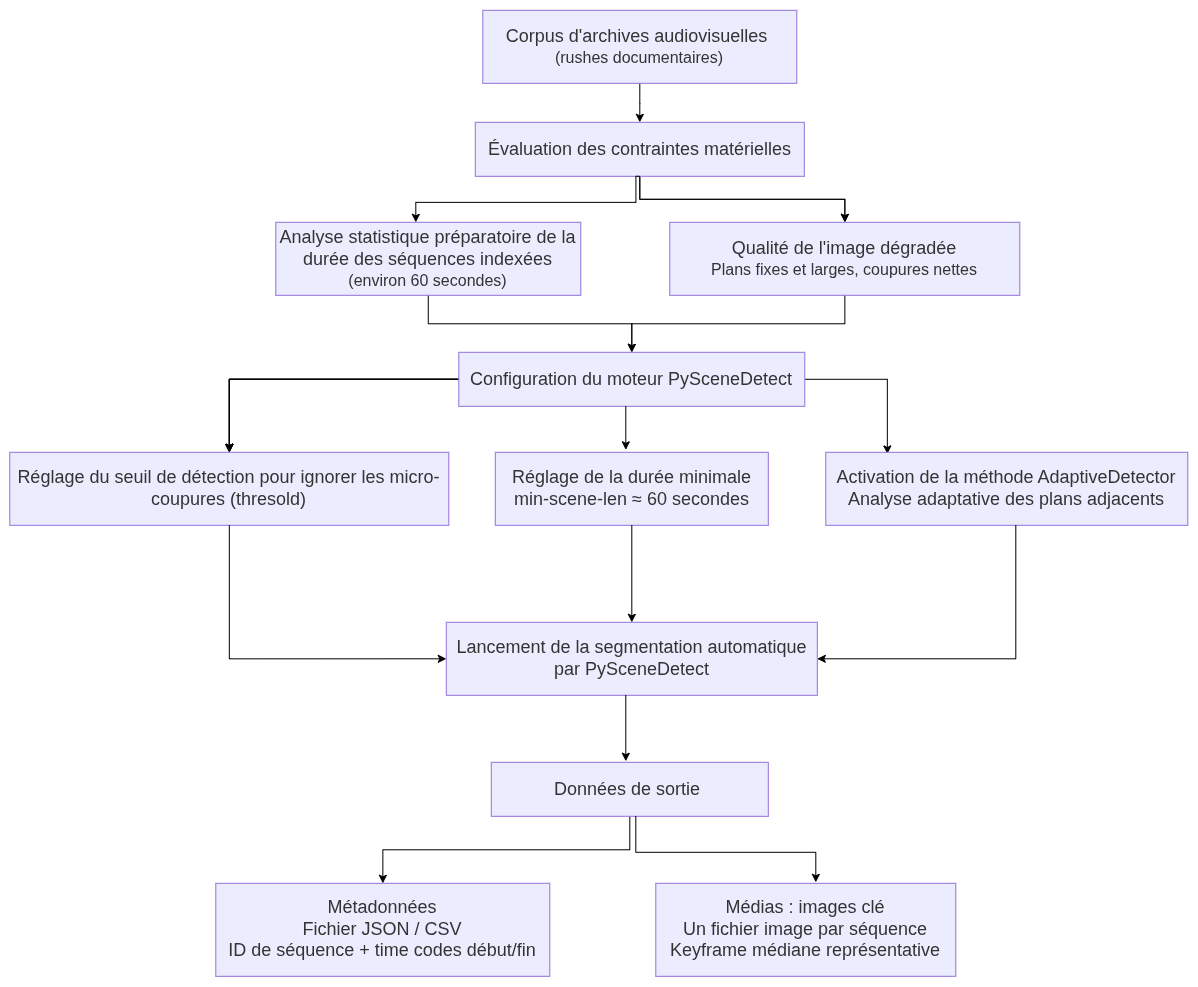
\includegraphics[width=1.0\textwidth]{images/pyscene.png} 
	
	\caption{Mise en application de \gls{pyscene}} 
	
	\label{figpyscene} 
	
\end{figure} 

Toutefois, si ce paramétrage permettrait une plus grande flexibilité pour la segmentation d’un flux vidéo en \gls{sequence}s, l’outil reste limité dans l’automatisation de cette tâche. D’une part l’outil est prévu pour la détection automatique de changement de plan, et d’autre part, une \gls{sequence} ne se définit pas seulement comme une caractéristique syntaxique du langage cinématographique, comme c'est le cas du plan, mais bien par une double caractéristique syntaxique et sémantique. En effet, un changement de séquence concrétise un choix narratif, matérialisé généralement par un changement d’espace-temps. C'est pourquoi, un outil dont l’automatisation est fondée sur des seuils mathématiques reste limité pour une telle tâche. Nous proposons alors de réaliser une analyse sémantique des \gls{sequence}s détectées, afin de ré-associer leur sens à ces coupures détectées automatiquement, tout en réutilisant les données produites : les \textit{times-codes} et l'image clé associés à chaque \gls{sequence}.  


Ainsi, la segmentation syntaxique effectuée par \gls{pyscene} constitue un “filtre”, c’est-à-dire un premier niveau dans notre chaîne d’indexation automatique des archives audiovisuelles \footcite{xin2023}. Les données issues de ce premier niveau permettent d’amoindrir le volume de données, caractéristique des fichiers vidéo, transmis aux algorithmes d’indexation automatique. Dès lors, les \gls{imgcle} produites par \gls{pyscene} peuvent être soumises à un modèle neuronal de détection d’objets tel que \gls{yolo} (\textit{You only look once}), afin d’extraire le sens de ces segments et leur rendre leur valeur sémantique. La sous-section suivante détaille la manière dont ce modèle, appliqué aux \gls{imgcle} issues des différentes \gls{sequence}, permet d’en extraire les caractéristiques sémantiques à des fins d’indexation.  




%Il est courant d’utiliser des modèles préentraînés sur un grand jeu de données et de le réajuster ensuite au jeu de données en question, au sein d’un contexte précis. \footcite{norindr2023} Ce modèle peut justement servir de modèle de caractéristiques à analyser sur les vidéos, un second entraînement, dans le contexte peut aider à l’affiner et à l’adapter au corpus spécifique. Le rendre d’abord familier au langage audiovisuel.  

%Malgré de grandes avancées dans le processing audiovisuel, avec des outils comme la computer vision appliquée à la vidéo, et la reconnaissance de discours automatique (ASR), ces outils restent largement inaccessibles et hors de portée pour les institutions patrimoniales. \footcite{noord2021}. Ils sont utilisés par des entreprises commerciales pour du montage vidéo par exemple. Le manque d'utilisation de ces outils dans le domaine des sciences humaines expliquent l'inexistance de données d'entraînement adaptées au secteur. \footcite{noord2021} 
%l'analyse vidéo par un processus humain prend un temps considérable, puiqu'il faut lire le fichier audiovisuel et en analyser les composants, le langage. Ainsi, l'indexation des archives audiovisuelles se cantonne souvent aux métadonnées, sans en exposer les données, le contenu.

%Et donc en pratique, comment appliquer le traitement audiovisuel à des corpus d'archives audiovisuelles patrimoniales ? 






%\subsubsection{entraîner ces outils et ces modèles}

%les modèles de détection neuronaux sont entrainés sur des datasets de clips courts. Or, la réalité auiovisuelle est bien différente. \footcite{pattichis2023} Des approches algorithmiques non neuronales ou hybrides seraient donc plus adaptées car fondée sur des calculs et des seuils matéhmatiques : plus stable. 

%détection des coupures : 
%approche algorithmique non neuronale (2SDS, pyscenedetect), (xin et attard) pipeline technique en 4 étapes (down sampling (miniaturisation), conversion en niveaux de gris, calcul d'empreinte numérique par hachage binaire des pixels, et calcul de la distance de Hamming pour marquer la rupture visuelle (xin2023)

%efficace sur les plans fixes et mvts lents 

%mettre en rapport avec les travaux d'Arnold  Tilton (2019), qui utilisent une méthode similaire combinant différences d'histogrammes et réduction de résolution des pixels (downsampling) pour mesurer les ruptures de palettes de couleurs et de luminosité d'une frame à l'autre, complétée par des règles logiques pour éviter les faux positifs lors des fondus (fade-in/fade-out).

%L'apport de l'IA (Vers la classification sémantique) : La détection brute des coupures ne suffit plus ; l'enjeu actuel est la Shot semantics (décrire le contenu d'un plan et sa typologie) (Arnold  Tilton, 2019).

%Le rôle des modèles (CNN et Détecteurs) : Pour analyser le contenu de ces plans, on utilise l'apprentissage supervisé (Supervised Learning), où des algorithmes apprennent à partir de données labellisées par l'humain (DeLua, 2024). C'est le cas des réseaux de neurones convolutifs (CNN) comme Faster R-CNN ou YOLO (un détecteur de type Single Shot qui prédit et classifie "en une seule fois") pour la détection d'objets ou de visages (Arnold  Tilton, 2019 ; Robert, 2026).

%Le méta-algorithme de classification : Arnold  Tilton (2019) montrent qu'en combinant la position des visages détectés et les coupures de plans, on peut créer un méta-algorithme capable de classifier automatiquement le type de plan (gros plan/close-up, plan amorce/over the shoulder), permettant de comprendre comment le cadrage construit le récit.

%\subsubsection{analyse du mouvement}

%au lieu d'utiliser des larges modèles qui tentent de tout classifier, plutot utiliser des modèles "low parameter", c'est-à-dire des modèles 3D-CNN légers, avec moins de paramètres dédiés à la reconnaissance d'une seule activité précise. prenennt moins de mémoire vidéo. \footcite{pattichis2023}

%stratégie de réduction de l'annotation humaine : slf supervised learning, semi supervised, active learning, zero shot \footcite{pattichis2023}

%confronter les architectures de réseaux de neurones (CNN vs. Transformers), introduire l'apprentissage non supervisé (Unsupervised Learning / DeepCluster),

%Les limites des CNN 2D classiques (comme ResNet) : ils analysent la vidéo comme des images discrètes et indépendantes, ignorant la continuité du mouvement \footcite{xin2023}. Se tourner vers les vision transformers : CLIP, ViViT (bergmann et al), mécanismes d'auto attention qui analysent l'intégralité d'une séquence

%Les modèles de Video Semantic Segmentation (VSS) et le dilemme entre les méthodes orientées "vitesse" (approche par keyframes peu précise) et orientées "précision" (TDNet, flux optique, mécanismes d'auto-attention) \footcite{zhou2022}.

%La gestion du coût de calcul : présentation de TDSNet (TFRM pour extraire les zones dynamiques par soustraction d'images consécutives, et MMRM pour pondérer selon la magnitude réelle du mouvement) \footcite{yuan2025}. règle ce dilemme 

%alternatives non supervisées : la supervision demande des données annotées (caron et al), l'apprentissage non supervisé (Unsupervised Learning) comme DeepCluster (Caron et al., 2018). Ce type de modèle regroupe les images ou frames similaires en "clusters" algorithmiques (via K-means) pour s'auto-entraîner sans intervention humaine (Caron et al., 2018). Si DeepCluster s'avère robuste face à des changements de distribution d'images (ce qui est prometteur pour des archives spécifiques), il présente deux limites majeures : il introduit des biais imprévisibles en remplaçant les labels par des métadonnées brutes (inacceptable pour la rigueur historienne) et a été conçu sur des bases gigantesques (ImageNet, 1.28 million d'images), le rendant difficilement transposable à des collections d'archives réduites (Caron et al., 2018 ; Norindr, 2023).

%infrastructure locale : amener l'algorithme aux données : C'est la discussion centrale de votre partie. Les outils d'AVP commerciaux (souvent basés sur le Cloud) sont inutilisables pour les archives en raison des droits de propriété intellectuelle et de la sécurité des données (van Noord et al., 2021). La solution réside dans des architectures locales comme DANE (projet CLARIAH), basées sur un système décentralisé de workers (van Noord et al., 2021). Ce type d'infrastructure produit des métadonnées exploitables, mais aussi des vecteurs de caractéristiques (représentations abstraites) ouvrant la voie à la recherche par similarité visuelle ou sonore (van Noord et al., 2021).

%La note finale sur l'explosion des données : L'indexation automatique par IA (comme avec DigInPix ou les modèles de type VLM) génère une masse d'informations locales phénoménale : les bases de données constituées peuvent être plus lourdes en taille que les fichiers vidéos d'origine (Moiraghi  Letessier, 2018).

%transition : nécessité d'un mapping vers le FRBR : faire correspondre la sortie de ces pipelines avec un modèle de données. 
\chapter{\label{II_2}Description et indexation automatique} 

%à rajouter pour faire la transition : %L'apport de l'IA (Vers la classification sémantique) : La détection brute des coupures ne suffit plus ; l'enjeu actuel est la Shot semantics (décrire le contenu d'un plan et sa typologie) (Arnold  Tilton, 2019).

La description automatique d’images peut être centrée sur de nombreux éléments au sein d'une \gls{sequence} de film : dialogues, ambiance sonore, visages, objets, spatialité des éléments, actions, émotions... Toutefois, la définition d’un processus au sein d’un logiciel de gestion des collections impose un cadrage défini des fonctionnalités. Le corpus patrimonial retenu pour notre étude, constitué de \gls{rush} muets des premiers temps, exclue d’emblée l’analyse automatique de caractéristiques sonores. L’analyse automatique se concentre donc exclusivement sur les caractéristiques visuelles de l’image. Deux approches coexistent alors, celle de l’identification des éléments dans l’image de manière précise, ou celle d’éventuellement générer des résumés automatiques sur ces séquences, à une échelle plus globale. Or, la seconde approche, fondée sur des grands modèles de langage, implique des architectures génératives couteuses et lourdes. Nous choisissons ainsi d’adopter la première, afin de garantir une indexation fiable et stable, plus légère, à travers la détection et l’identification d’objets sur les \gls{imgcle}préalablement extraites. Cette tâche peut être réalisée par des architectures de réseaux de neurones relativement légers, pouvant extraire des concepts directement indexables au sein du logiciel.  




\section{\label{II_2_A}Outils utilisés}

Si pour la tâche de segmentation automatique, nous avons écarté les architectures de modèles fondés sur des réseaux de neurones, la reconnaissance d'objets dans l'image suppose une prédiction fondée sur un apprentissage machine profond des réseaux de neurones. En effet, la plupart des outils de reconnaissance d'objets dans l'image sont fondés sur des modèles de réseaux de neurones convolutifs (CNN) dont nous avons exposé le fonctionnement dans la section précédente. Dans le domaine du patrimoine, dont le logiciel de Skinsoft gère les données des institutions, se pose la question d'une infrastructure adaptée qui permet d'assurer la sécurité des données produites. Les solutions commerciales d'analyse automatique sont pour la plupart fondées sur un Cloud externe qui implique le déplacement des données. Ces solutions sont inadaptées au contexte d'analyse de données patrimoniales en raison de propriété intellectuelle et de sécurité. Ainsi, le principe retenu afin de guider notre choix d'outil est celui d'"amener l'algorithme aux données [Traduction personnelle]" \footnote{\textit{"bring algorithms to the data"}}, via un développement local interne des modèles d'analyse \footcite{noord2021}. Afin de répondre à cette contrainte, notre choix s'est trouné vers des modèles en libre accès. Nous détaillerons dans cette section l’utilisation de l’architecture \gls{yolo}, une série d’algorithmes dédiés à la détection d’objets visuels dans les images et les flux vidéo, et fondé sur les réseaux neuronaux convolutifs, développé par Joseph Redmond en 2015, puis repris par Ultralytics en 2020 \footcite{talbi2025}. 
C’est l’un des outils de détection d’objets les plus documentés, y compris dans le domaine des sciences humaines et du patrimoine. Fondé sur la \gls{Vision par ordinateur} et entraîné grâce à des méthodes d'\gls{Apprentissage profond}, \gls{yolo} est en accès libre, et permet notamment la détection d'objets et la classification d'images, permettant ainsi de poser les bases d’une indexation \footcite{jocher2022}. Le modèle extrait dans un premier temps les caractéristiques visuelles de l'image qui lui est donnée, les agrège, afin de finalement proposer une détection d'objets \footcite{norindr2023}. Les versions récentes du modèle telles que YoLo12 ne sont désormais plus seulement basées sur des \gls{cnn} mais sur des mécanismes d'auto-attention, similaires à ceux des \gls{Transformers} dont nous avions évoqué l'architecture \footcite{2025b}. Toutefois, comme nous l'avions évoqué, cette architecture demande une consommation de mémoire élevée et une puissance de calcul lourde \footcite{2025b}. Ultralytics, créateur du modèle, recommande des versions moins avancées pour une mise en application rapide, telles que la version Yolov8, uniquement fondée sur un réseau de neurones convolutif \footcite{2023c}. Yolov8 propose une version optimisée de cette architecture en trois temps : extraction, aggrégation, et détection \footcite{yaseen2024}. Le modèle se caractérise par sa capacité à analyser l'image en une seule fois, contrairement à d'autres modèles dont les résultats impliquent plusieurs analyses de certaines parties de l'image \footcite{redmon2016}.  
Si la détection d’objets prévue par \gls{yolo} peut être appliqué à des flux vidéo, nous souhaitons l'intégrer comme composant complémentaire au processus de segmentation précédemment décrit. De fait, il être pertinent de réutiliser l'image clé fixe, produite et sauvegardée par l'outil pyscenedetect, associée à chaque séquence, afin de la faire analyser par le modèle. Ceci permettrait de réduire le temps de calcul du processus et d'améliorer l'efficacité des prédictions, puisque le modèle reçoit un minimum d’informations.  
Ainsi, l’application du modèle \gls{yolo} s’impose comme la suite logique du pipeline de segmentation détaillé précédemment, afin d’indexer les segments produits, via l’utilisation des \gls{imgcle}. Si le premier processus de segmentation produit des données temporelles associées à chaque séquence sous la forme de time codes, \gls{yolo} produit des données sémantiques sur ces mêmes séquences. À l'issue de l'analyse d'une \gls{imgcle}, le modèle \gls{yolo} est capable de produire trois types de données : des étiquettes sur les objets identifiés, un score de confiance qui indique l'indice de certitude concernant la prédiction, des coordonnées spatiales de localisation de l'objet détecté dans l'image \footcite{redmon2016}. Les étiquettes produites sur les objets identifiés, permettant de décrire les caractéristiques de l’image, pourront être indexées comme des mots-clés au sein du logiciel de gestion des collections. Le processus de détection d'objets prévu par \gls{yolo} à partir de l'image clé peut être schématisé ainsi : 

\begin{figure}[H] 
	
	\centering 
	
	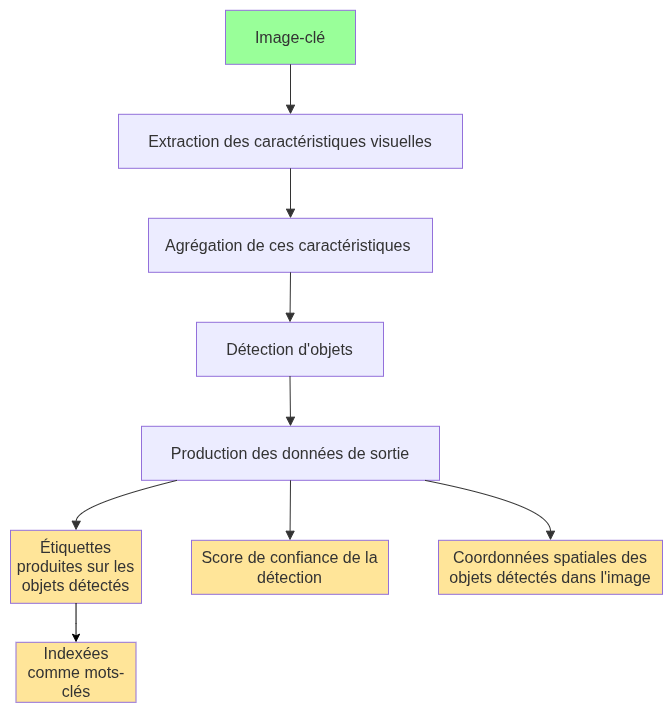
\includegraphics[width=0.7\textwidth]{images/yolo.png} 
	
	\caption{Processus de détection d'objets de \gls{yolo}} 
	
	\label{fig:yolo} 
	
\end{figure}

Les mots-clés produits à partir des étiquettes sont ensuite associés aux time-codes de chaque séquence détectée. Ainsi, chaque séquence contiendrait les données suivantes : des time codes qui l'identifient comme extrait, des étiquettes/mots-clés sur les objets qu'elle contient, et des données qui permettraient aux utilisateurs de vérifier la prédiction et de la valider. Le score de confiance produit par le modèle, permet en effet d'indiquer à l'utilisateur la certitude de l'étiquette associée à tel objet détecté. De même, les coordonnées spatiales de l’étiquette produite permettent à l’utilisateur de vérifier dans l'image si l'étiquette produite est associée au bon objet.  
\section{\label{II_2_B}Entraînement}

L'analyse automatique du contenu des images repose donc sur les architectures des \gls{cnn}, fondées sur des méthodes d'\gls{Apprentissage profond}, dont YOLO est un exemple concret. Toutefois, les algorithmes fondés sur l'\gls{Apprentissage profond} subissent généralement un entraînement supplémentaire afin d'analyse adéquatement le contenu des images en fonction d'un contexte donné. Deux approches méthologiques d'entraînement peuvent être appliquées, l'\gls{appsup} et l'\gls{appnonsup}. L'\gls{appsup} est fondé sur l'utilisation de données annotées pour l'amélioration des prédictions du modèle d'analyse d'image, tandis que l'\gls{appnonsup} exécute des tâches d'analyse et de classification à partir de données brutes, non annotées \footcite{delua2024}. Toutefois, l'\gls{appnonsup} ne permet pas d'adapter suffisamment le modèle de détection d'objets au corpus d'images spécifique étudié. En effet, si Yolov8 a toutefois fait l'objet d'un pré-entraînement en amont de sa mise à disposition, sur le jeu de données COCO, ce dernier, composé de 200 000 images annotées, reste généraliste et adapté à la détection d'objets communs et contemporain\footcite{2023b}. Or, l'efficacité des modèles basés sur l'\gls{Apprentissage profond} sur un corpus spécifique dépend fondamentalement de nature et de la qualité de leur données d'entraînement. 
Au sein des sous sections suivantes, nous prendrons comme exemple d’application le projet des archives britanniques en ligne, qui propose une chaine de traitement pour la détection d’objet basée sur l'\gls{Apprentissage profond} et la supervision humaine \footcite{kasturi2024}. Le projet, à travers la mise en place d'une supervision au sein du processus d'analyse par le modèle, propose de mettre en application le concept de \gls{hil} \footcite{kasturi2024}.
Le corpus étudié, caractérisé par l'ancienneté de ses images en fait un corpus d’images spécifique sur lequel l’algorithme doit subir un entraînement supplémentaire, supervisé. Afin d'adapter le modèle à notre corpus et ainsi d'en améliorer l'efficacité, une phase de pré traitement est nécessaire sur les données du corpus, au cours de laquelle des images sont sélectionnées afin d’être annotées pour être pré-testées par le modèle \footcite{kasturi2024}. La supervision humaine est déterminante dans ce processus, particulièrement dans le cas d’analyse de corpus inédits sur lesquels l’algorithme reste à entraîner \footcite{kasturi2024}. 
Les british online archives implémentent l'adaptation du modèle par la pré selection d'un nombre d'images définis, annotées manuellement à l'aide de la plateforme \gls{labels} \footcite{kasturi2024}. \gls{labels} est une plateforme open source déployable localement, qui permet ainsi de respecter la protection des données analysées \footcite{zotero-item-783}.
Afin d'éviter l'annotation manuelle de l'ensemble des \gls{imgcle} issues du processus de segmentation, il peut être envisagé d'exécuter au préalable \gls{yolo} depuis \gls{labels} sur l'ensemble des \gls{imgcle} du corpus afin de générer une base de prédictions \footcite{development2025}. Les détections brutes générées peuvent ensuite être importées au sein de la plateforme comme une couche d'annotation préalable à partir de laquelle affiner le modèle. Au sein de \gls{labels}, les prédictions s'affichent sous la forme de \textit{bounding boxes}, c'est-à-dire de boîtes englobantes autour des objets detectés dans l'image, avec le score de confiance qui y est associé \footcite{kasturi2024}. Le paramètre [choices] permet au modèle de proposer une classification sur les objets détectés, c'est-à-dire un mot clé \footcite{zotero-item-785}. Afin de focaliser la supervision du modèle sur les éléments les plus pertinents, il peut être décidé de ré annoter les images dont la détection est jugée incertaine par le modèle via un score de confiance en dessous du seuil minimal attendu \footcite{development2025}. Les archives brittaniques préconisent également la uppression des boites englobantes redondantes afin de sélectionner celles qui sont les plus pertinentes pour la supervision \footcite{kasturi2024}. Dans \gls{labels}, les utilisateurs (une équipe technique dans le cas de Skinsoft) examinent les prédictions ainsi générées sur les images, rectifient si besoin la définition des "boites" et la classification associée \footcite{kasturi2024}. Les données ainsi corrigées sont exportées au format \gls{yolo} depuis \gls{labels}, puis réinjectées dans la chaîne de réentraînement du modèle afin d'améliorer les performances en accord avec le corpus \footcite{kasturi2024}.
Cette méthode s'appuie sur le transfert d’apprentissage (transfert learning), qui consiste à \textit{fine tuner} un modèle existant, c’est-à-dire de l’affiner, afin de l'adapter au corpus analysé \footcite{bhargav2019}. À défaut de réentraîner le modèle dans sa globalité, les prédictions réalisées à partir du jeu de données d'entraînement COCO sont conservées puis spécialisées sur un corpus donné \footcite{bhargav2019}. L'affinage du modèle via la rectification et l'annotation des données, constitue une étape de prétraitement, en amont de l’analyse des données, afin d'améliorer l'efficacité de la détection d’objets \footcite{kasturi2024}.
Cette étape de pré-traitement, avant le processus d'analyse, implique la définition des types de mots clés souhaités, pour l'indexation des séquences. En effet, les étiquettes associées aux objets au sein des images correspondent aux mots-clés qui seront prédits par le modèle lors de l’analyse. Dans le cadre du corpus étudié, il est pertinent d’extraire les mots-clés déjà indexés sur les \gls{sequence} au sein du logiciel. Ces mots-clés varient selon le contenu de l’image et peuvent, par exemple, être les suivants : affiche, foule, policier, gendarme, drapeau, etc. Ces mots-clés, tout comme le jeu de données COCO, sont assez génériques. De fait, le pré traitement est avant tout utile pour l’entraînement du modèle à pouvoir détecter des objets au sein d’images dont la qualité est compromise.   
\section{\label{II_2_C}Processus de validation technique}

%Poursuite de l'application du concept HIL 

Afin de gérer les essais-erreurs de l'affinage du modèle sur les données spécifiques du corpus, il est pertinent de mettre en place un processus de validation technique du traitement. Ce processus permettrait d'une part de valider les résultats du modèle, et d’autre part, d'assurer la concordance entre les données produites par le modèle avec les données déjà existantes au sein du logiciel.

La validation des prédictions du modèle peut être effectuée au sein de la plateforme \gls{labels}. Les archives brittaniques proposent que le jeu de données test utilisé précédemment afin de corriger les prédictions, soit distinct d'un second jeu de données test, dédié à l'évaluation des performances du modèle, à différents niveaux de supervision humaine \footcite{kasturi2024}. Sur ce second jeu de données, sont notamment intégrées des métadonnées de supervision humaine. En effet, Kasturi explique l'introduction des notations "HIL-10 \%, HIL-15 \% et HIL-20 \%, qui signifient respectivement que les utilisateurs ont corrigé 10 \%, 15 \% et 20 \% des boîtes englobantes prédites peu performantes dans l’ensemble de données de test." \footcite{kasturi2024}. (traduction de :  HIL-10\%, HIL-15\%, and HIL-20\%, which signify that users have corrected 10\%, 15\%, and 20\% of poorly performing predicted bounding boxes in the test dataset, respectively). Les données corrigées manuellement remplacent ensuite certaines images au hasard dans le premier jeu de données d'apprentissage, contituant un nouveau jeu de données d'entraînement sur lequel le modèle s'affine \footcite{kasturi2024}. 
Le modèle ainsi affiné est finalement exécuté sur le second jeu de données, corrigé selon différents niveaux d'intervention humaine \footcite{kasturi2024}. Pour chaque niveau de supervision, sont analysés les "scores moyens d’Intersection over Union (mIOU) et de précision moyenne (mAP), ainsi que de la précision et du rappel" \footcite{kasturi2024}. 
Les résultats obtenus montrent que les performances du modèle s'améliorent considérablement à mesure que le pourcentage d'images corrigées manuellement augmente \footcite{kasturi2024}. En effet, l'enrichissement du jeu de données permet au modèle d'appréhender l'analyse des images de manière plus précise. L'auteur note toutefois la nécessité de poursuivre l'évaluation du modèle sur d'autres données afin de vérifier son adaptabilité et ses performances pour la détection d'autres types d'objets \footcite{kasturi2024}. En effet, le modèle devrait être ré entraîné constamment, à mesure qu'il soit exécuté sur de nouvelles données. (Active learning)


De plus, le processus de validation technique implique également la validation de l'indexation des données produites au sein du logiciel, en adéquation avec les règles métier en place. Au sein de l’espace de travail S-Movies dédié au corpus étudié, l'indexation des mots-clés est contrôlée par le thésaurus "keyword". Or, le modèle \gls{yolo} est nativement pré entraîné sur un jeu de données généraliste dont les étiquettes produites ne correspondront pas directement aux autorités indexées dans la base de données. Deux cas peuvent être gérés par l'utilisateur côté technique. D'une part, les mots-clés produits par le modèle peuvent déjà être indexés sous une forme contrôlée au sein du logiciel. Dans ce cas, il revient à l'utilisateur de vérifier que les mots-clés générés par le modèle concordent avec la forme indexée contrôlée au sein du logiciel. À terme, cette tâche de validation pourra être gérée par un LLM, un grand modèle de langage, déjà employé par Skinsoft pour un outil de recherche en langage naturel par exemple. Ce grand modèle de langage pourra être capable, à partir du thésaurus indexé dans le logiciel, de valider les formes contrôlées des mots-clés générés par \gls{yolo}. Pour cela, un mapping (tableau de corespondance) pourra être fourni au LLM entre les mots-clés que le modèle peut potentiellement générer, et leur forme contrôlée dans le thésaurus. Nous avons effectivement déjà élaboré un tel tableau au cours de notre stage dans le cadre de la mise en place de l'intelligence artificielle pour d'autres tâches, notamment la mise en place d'une recherche en langage naturel. Pour cette tâche tout à fait différente que celle que nous décrivons dans ce mémoire, nous avons effectué une table de correspondance entre les champs contrôlés pouvant être requêtés dans le logiciel et leur définition en langage naturel, préparant ainsi la gestion de synonymes et de termes employés par l'utilisateur potentiellement pour requêter ces champs. Sur le même principe, nous pourrions mettre en place une table de correspondance afin d'assurer la validation des données produites et d'assurer \textit{in fine} leur indexation au sein de l'application. Un calcul de similarité aide le LLM à repérer les termes simiaires et els rapprocher de leur forme contrôlée.
D'autre part, si les mots clés n'existent pas sous une forme contrôlée au sein du thésaurus et qu'aucune correspondance n'est détectée, un nouveau terme de thésaurus pourra être créé au sein du logiciel, avec l'accord de l'utilisateur.

%à ajouter : Named Entity Linking – NEL compare les entités trouvées avec les données normatives). L'algorithme ou le modèle mathématique effectue une classification multi-labels. Il se base sur des concepts statistiques tels que TF/IDF (Term Frequency/Inverted Document Frequency). \footcite{zotero-item-584}







La \gls{segtemp} ne se suffit pas à elle-même, mais nécessite une description du contenu des segments, afin d'en rétablir la qualité de \gls{sequence}, unité audiovisuelle à la fois syntaxique et sémiotique. L'approche retenue afin de décrire automatiquement le contenu de ces segments est celle de l'implémentation du modèle YOLOv8, dont le temps de calcul et de prédiction est réduit par son application aux \gls{imgcle} produites par la segmentation. L'efficacité du processus repose sur la supervision et la validation humaine, côté technique, des prédictions produites par le modèle, en accord avec les règles métier du logiciel. Toutefois, l'indexation définitive au sein du logiciel doit être validée par l'utilisateur métier via une interface dédiée, et au sein du modèle de données FRBR. 








%généralement, un algorithme de machine learning comprend trois étapes : data pre processing, data modelling, process optimisation. Dans le pre processing : humain requis pour transformer des données non structurées en données structurées et annotées \footcite{kasturi2024}

 











\chapter{\label{II_3}Indexation des données produites au sein du modèle de données} 
\titreEntete{Indexation des données produites}

L’objet de notre étude est le reversement des données produites par l’indexation automatique au sein du modèle FRBR, adapté aux archives audiovisuelles. Si les outils d’extraction automatique tels que YOLOv8, nécessitent un réentrainement spécifique au corpus étudié, une seconde difficulté s'impose, celle de l'alignement de ces données avec un modèle de données personnalisé. Le modèle de données FRBR est, en effet, configuré selon les besoins métier de chaque institution et conditionne l’organisation des données pour l’utilisateur au sein de l’interface. Dès lors, comment reverser des données produites automatiquement, au sein d’un modèle de données configurable ? Ce reversement concrétise en effet l’indexation automatique, puisque les données deviennent visibles et requêtables par les utilisateurs, au sein de l'interface du logiciel. 

%Faire le lien avec le NLP le plus possible : le NLP pourra être étendu pour la recherche de contenus visuels  

%Yolo est une IA discriminative 


\section{\label{II_3_A}Reversement des données au sein du FRBR} 

Le processus automatisé proposé repose sur l'exécution de deux phases : d'une part la segmentation temporelle d'un flux vidéo (géérant des time codes et des images-clé), et d'autre part la détection et la classification d'objets (générant des mots-clés). L'enjeu est de prévoir la structuration de ces différents types de données, chiffrées et textuelles, au sein du modèle FRBR existant. 

%Certains outils ont déjà été développés dans d’autres applications de gestion des collections afin d’effectuer ce reversement de manière automatique : Wedia, Keepeek, Einden, MomaSoft “classent automatiquement les images et vidéos en leur attribuant les métadonnées appropriées.” \footcite{zotero-item-732}

Les outils automatiques utilisés lors du processus ont extrait des données depuis un média, associé au niveau de l'item numérique au sein du modèle de données préexistant. Or, le niveau item contient des éléments de description matérielle techniques, alors que les mots-clés et repères temporels relèvent d'une description intelectuelle et syntaxique. Dès lors, la création d'une entité intelectuelle dédiée à la séquence s'impose. 
Afin d'illustrer l'intégration d'une entité de description intermédiaire, entre l'oeuvre et l'item numérique, prenons l'exemple de la plateforme Okapi (Open and Knowledge-based Annotation and Publishing Interface), développée par le département Recherche et Innovation de l'\gls{ina} \footcite{lalande2022}. Afin de favoriser la description collaborative de contenus multimédias, la plateforme offre la possibilité aux utilisateurs de concevoir des modèles de description personnalisés \footcite{lalande2022}. La plateforme permet notamment de séparer l'extrait audiovisuel du média, dont il constitue un niveau descriptif propre. Une strate supplémentaire de description est ainsi dédiée à la description intellectuelle du média. Le modèle FRBR tel que nous l'avons décrit ne propose, a priori, pas d'entité descriptive dédiée à la séquence. L'entité "d'agrégats", proposée par le manuel de la \gls{fiaf} pourrait y correspondre. Toutefois, ceux-ci “sont conçus et créés dès le début pour rassembler plusieurs composantes individuelles formant un tout." \footcite{zotero-item-646}. Or, au sein du corpus étudié, les rushes ne font pas partie d'un montage. Toute segmentation est une interprétation a posteriori de la construction de l’archive, et donc un remontage. L'entité de "fragment d'expression" proposé par l'IFLA au sein du modèle FRBR bibliographique semble plus adéquate \footcite{iflastandards.info2026}. L’\gls{IFLA} définit le fragment comme “des parties d’expressions qui ne constituent pas elles-mêmes des expressions autonomes.[...] Un « Fragment d’expression » n’est identifié qu’en fonction de son occurrence au sein d’un tout connu ou supposé.” \footcite{iflastandards.info2026}. Cette entité semble correspondre à la notion de séquences telle que nous l'avons décrite. Elle serait rattachée à l’Oeuvre, conformément à l’adaptation du FRBR par les recommandations de la FIAF, et permettrait le reversement spécifique des times-codes et mots-clés. La figure \ref{figfragment} ci-dessous illustre l'intégration de l'entité du fragment d'oeuvre au modèle de données existant. 

\begin{figure}[htbp] 
	
	\centering 
	
	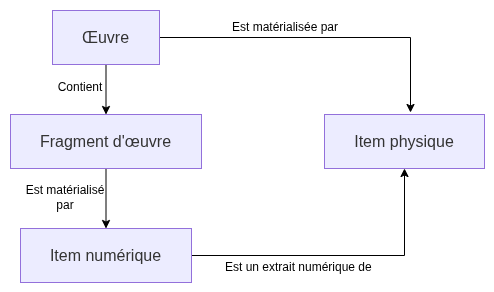
\includegraphics[width=0.7\textwidth]{images/fragment_frbr.png} 
	
	\caption{Intégration du Fragment au modèle de données} 
	
	\label{figfragment} 
	
\end{figure} 

Au sein de la plateforme Okapi, la création d'une entité intermédiaire de description, permet aux données descriptives produites à partir du média, d'être reversées au sein d'un niveau parent essentiellement descriptif, celui de l'extrait. Au sein du modèle de données existant, adapté au corpus étudié, les time codes et les mots-clés sont déjà indexés manuellement en tant que données au sein de l’application. En effet, les times codes sont renseignés au niveau de l'item numérique, dans un champ notes, et l'item comporte le champ type renseigné par la valeur “fichier time codé”, afin de signifier sa qualité d'extrait. De plus, les mots-clés sont renseignés au niveau de l’indexation de l’œuvre, donc du rush original. La modélisation de la segmentation au sein du modèle actuel implique un nombre conséquent de relations entre les éléments, complexifiant ainsi la navigation de l'utilisateur. En effet, une notice d'item physique renseigne tous les extraits numériques (items numériques) qui lui sont liés. L’item numérique (segment) renseigne le film physique duquel il est extrait, tandis que le niveau œuvre renseigne uniquement les extraits numériques qui lui sont associés. 
La création d’une nouvelle entité simplifierait la navigation au sein de l'interface et permettrait de séparer la description en différents niveaux, intellectuel et technique, conformément aux principes du FRBR. La nouvelle entité de fragments permettrait éventuellement de préciser un contexte de segmentation et des champs dédiés aux mots clés et aux time codes. Le tableau \ref{tab:reversement_metadonnees_frbr} ci-dessous illustre la répartition de la description entre le fragment d'Oeuvre et l'item numérique. Pour des raisons de clarté, d'autres données descriptives ont été intégrées afin d'illustrer la répartition entre la description intellectuelle et matérielle. 

\begin{table}[H]
	\centering
	\small
	\renewcommand{\arraystretch}{1.3}
	\begin{tabular}{|p{3.8cm}|p{4.2cm}|p{6.4cm}|}
		\hline
		\textbf{Entité FRBR} & \textbf{Champ / Attribut} & \textbf{Exemples de valeurs} \\
		\hline
		\multirow{6}{=}{\textbf{Fragment d’Oeuvre} \newline \textit{(Description intellectuelle)}} 
		& Contexte & Segmentation automatique de tel item physique \\ \cline{2-3}
		& Description générale & Description du contenu sémantique de la séquence \\ \cline{2-3}
		& Processus de segmentation & Automatique (Outil utilisé et paramètres appliqués) \\ \cline{2-3}
		& Time codes & Time codes de début et de fin de la séquence \\ \cline{2-3}
		& Mots-clés & Mots-clés extraits par YOLO \\ \cline{2-3}
		& Image-clé associée & Lien direct vers le fichier de l'image-clé \\ \cline{2-3}
		& Oeuvre parente & Identifiant de l'oeuvre associée, lien direct vers la notice \\ \cline{2-3}
		& Item physique associé & Identifiant de l'item physique associé dont est tirée la séquence, lien direct vers la notice \\ \cline{2-3}
		& Item numérique associé & Identifiant de l'item numérique associé, lien direct vers la notice \\ 
		\hline
		\multirow{3}{=}{\textbf{Item Numérique} \newline \textit{(Description technique et matérielle)}} 
		& Fragment associé & Identifiant du fragment associé, lien direct vers la notice \\ \cline{2-3}
		& Données techniques & Résolution de l'image, taille, format \\ \cline{2-3}
		& Données de conservation & Emplacement, contenant \\ \cline{2-3}
		& Média associé & fichier média de la séquence \\ \cline{2-3}
		\hline
	\end{tabular}
	\caption{Attributs et exemples de valeurs associées aux entités Fragment d'Expression et Item Numérique.}
	\label{tab:reversement_metadonnees_frbr}
\end{table}

Les métadonnées automatiquement produites seraient intégrées au niveau du fragment, tandis que l'item numérique contiendrait le média et les données techniques. 
Une difficulté subsiste toutefois. En effet, les processus s'exécutent au niveau du fichier numérique et de son média, tandis que les métadonnées produites doivent pouvoir enrichir un niveau descriptif supérieur, celui du fragment. Dexu configurations peuvent être envisagées afin d'opérer ce reversement automatiquement. D'une part, l'application gère actuellement l'héritage des données d'un niveau supérieur à un niveau inférieur via la configuration de méta-masques, qui ciblent les niveaux iférieurs au sein desquels reverser les données. Néanmoins, le processus automatisé décrit impliquerait la configuration de masques ascendants, permettant de reverser des métadonnées générées au niveau de l'item, vers l'entité de fragment. Cette configuration complexifie toutefois la compréhension du modèle de données.
D'autre part, pourrait être envisagé la mise en place d'un tableau de correspondance ou d'un script permettant d'associer les sorties de données du processus aux entités dans lesquelles elles doivent être injectées. 
Une fois la modélisation du transfert établie entre les métadonnées automatiquement produites, et le modèle de données existant, le reversement définitif est toutefois laissé à l'utilisateur métier, au sein de l'interface du logiciel. 
%À l’ingest : données interdépendantes entre la description d’un item numérique et de son média. Mentionner la relation nouvelle sur l’item numérique et son média : facilite les choses pour le reversement  
%Pour les times codes, des champs dédiés devrons être prévus sous le champ film associé.  
%Faire un schéma de métadonnées pour pouvoir adapter les données aux normes du logiciel via des connecteurs par exemple.  

\section{\label{II_3_B}Proposer une interface de validation pour l'utilisateur} 

Si la redéfinition du modèle \gls{FRBR} s'effectue en \textit{backend} de l’application, par les équipes techniques et les équipes métiers du logiciel, afin de préparer l’implémentation de processus automatiques, les étapes de ces processus doivent toutefois être restituées au sein de l'interface auprès de l'utilisateur métier. Afin de donner à l'utilisateur le rôle de validation finale sur les données produites, l'espace de travail S-Movies doit permettre de visualiser les résultats afin de les valider. 

\subsection{Un enjeu de transparence}

En effet, dans le cadre de l'implémentation de fonctionnalités automatiques, fondées sur l'intelligence artificielle, la \gls{cnil} recommande que les utilisateurs soient familiarisés au fonctionnement et aux limites de ces outils, par exemple “la manière dont sont produites les sorties, les éventuels transferts de données, ainsi que les usages autorisés et les usages interdits." \footcite{zotero-item-729}. Ces informations pourraient notamment guider l’utilisateur pour la validation des données produites par les modèles. Si l'exposition de ces étapes peut être effectuée au sein de modes d'emploi dédiés, comme Skinsoft le prévoit déjà, les informations relatives aux fonctionnalités automatiques devront toutefois être directement intégrées à l’interface pour un souci de transparence. Ainsi, la \gls{cnil} recommande que "l’intégration de briques d’IA générative dans un système d’information (SI) devrait être pensée avec des éléments de design informant clairement les utilisateurs de l’origine de la proposition [...]." \footcite{zotero-item-729}.
De plus, en cas de non-validation des données produites par l'utilisateur, il pourrait être pertinent de proposer "un point de contact pour remonter des problèmes ou des difficultés d’ordre éthique"\footcite{zotero-item-729}. L’interface devra ainsi prévoir un formulaire décrivant la raison du refus des données, envoyé à l’équipe technique afin que l'algorithme puisse être amélioré, voire affiné. Au cours de notre stage, un système similaire a été proposé afin de prévoir la gestion des erreurs d'un outil de recherche en langage naturel, visible en Annexe B (\ref{annexe_B}). Un formulaire est prévu pour l'utilisateur en cas de résultats non pertinents pour que le processus soit amélioré.

\subsection{Développer une interface dédiée à la validation de l'utilisateur}
Si notre étude ne relève pas de l'\gls{ia} générative, il est toutefois pertinent d'offrir à l'utilisateur un niveau de transparence maximal au sein de l'interface, via la viualisation des données produites et leur validation finale. À l'image des deux phases de traitement automatiques développées dans les sections précédentes (segmentation et classification), la validation côté interface pourra prendre la forme de deux phases de décision. Il pourra d'abord être demandé à l'utilisateur d'actionner ou non le processus de segmentation puis de le valider ou de l'invalider. Une fois le processus de segmentation finalisé, l'utilisateur pourra décider de déclencher le processus de détection d'objets sur les segments produits, puis de finalement les modifier ou de les valider.
Afin de concrétiser le processus de validation côté interface, nous nous appuyons sur l'exemple de la plateforme Amalia.js, développée par l'\gls{ina} en 2015, conçue pour visualiser les résultats d’algorithmes d’analyse audiovisuelle \footcite{zotero-item-740}. Le besoin à l'origine d'Amalia.js est donc de permettre de visualiser les résultats divers issus de pipelines d'automatisation \footcite{herve2015}. Cette interface permettrait d'une part de visualiser les résultats et d'autre part, de vérifier la conformité des données produites en lien avec les standards métiers en vigueur au sein du logiciel \footcite{herve2015}. L'interface permet également d’annoter directement le flux vidéo afin de corriger les données produites \footcite{herve2015}. La correction effectuée par l'utilisateur  permet de constituer des données d'entraînement supplémentaires afin d'améliorer les algorithmes d'indexation automatique \footcite{herve2015}. 
Amalia.js intègre notamment un \textit{plugin} de \textit{timeline} pour l'affichage des segments temporels et des images-clés associées, ainsi qu'un \textit{plugin} de superposition (\textit{overlay}) qui permettrait l'affichage de l'encadrement des objets détectés \footcite{zotero-item-740}.
Plutôt que de développer deux modules distincts, cette logique pourrait être combinée au sein de S-Movies sous la forme d'un module d'édition des données. Ce module présenterait d'abord à l'utilisateur la ligne temporelle des séquences associées aux images-clés, puis après leur validation, le module prévoierait l'ouverture d'une fenêtre d'édition latérale contenant les propositions de mots-clés et les objets détectés entourés au sein des images-clés. Ce module d'édition s'inspire du \textit{plugin} \textit{Editor} au sein d'Amalia.js dont la figure \ref{figamalia} ci-dessous ilustre la disposition : 

\begin{figure}[H] 
	
	\centering 
	
	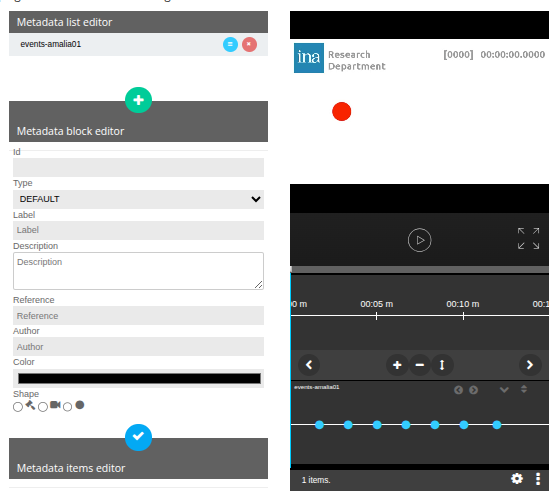
\includegraphics[width=1.0\textwidth]{images/amalia.png} 
	
	\caption{\textit{Plugin Editor} dans Amalia.js \footcite{zotero-item-794}} 
	
	\label{figamalia} 
	
\end{figure}

En cas de modification par l'utilisateur, l'interface pourrait enregistrer les données validées, tout en les envoyant en \textit{backend}, afin que le processus soit amélioré. 
Le développement de l'interface serait ainsi conforme à la mise en place d'une automatisation facilitatrice de la création de données, en incitant l'utilisateur "à vérifier les données fournies en entrée et la qualité des sorties" \footcite{zotero-item-729}.

\subsection{Déroulé du processus de validation}

Concrètement, en \textit{frontend}, dans l’interface de l’application prévue pour l’utilisateur, le processus suivant peut-être imaginé, illustré par un diagramme de décision (\ref{fig:validation}):

\begin{figure}[H] 
	
	\centering 
	
	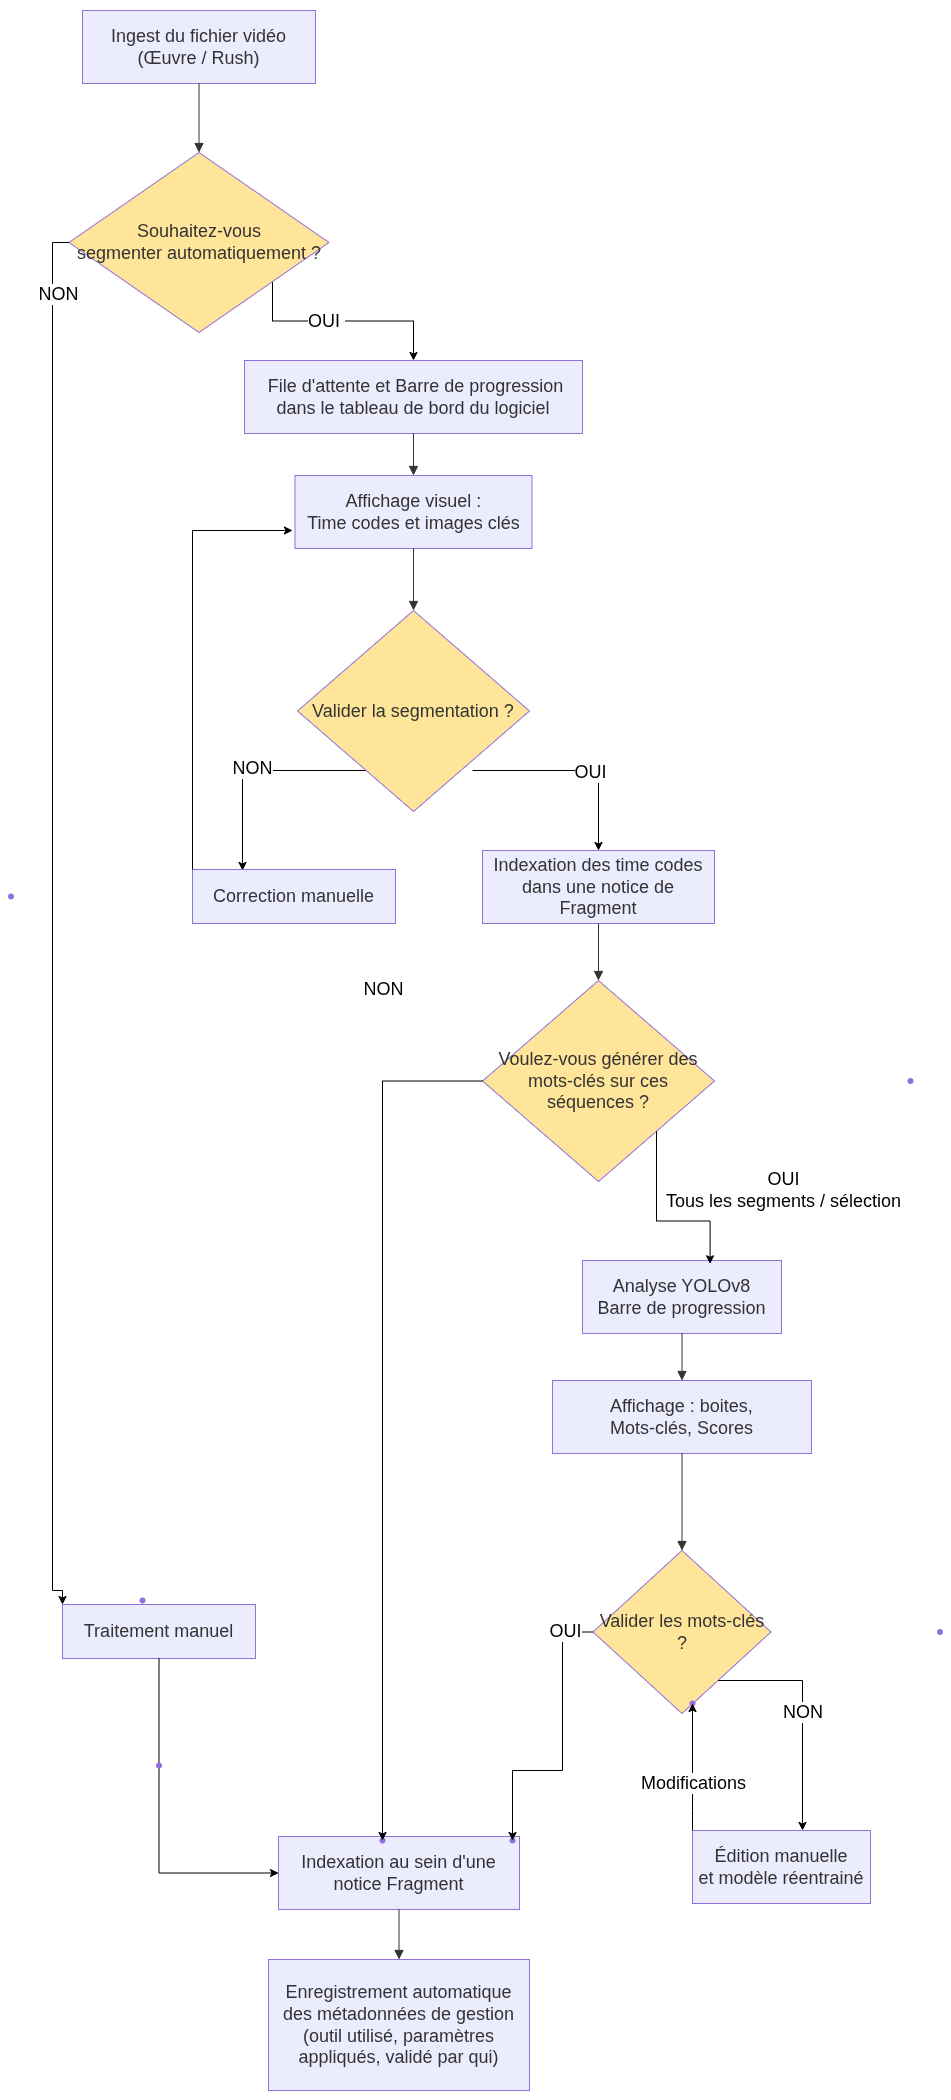
\includegraphics[width=0.6\textwidth]{images/validation.png} 
	
	\caption{Processus de validation de l'utilisateur métier} 
	
	\label{fig:validation} 
	
\end{figure}

Ce processus permet de laisser l'utilisateur métier décider de l'indexation des données via l'actionnage ou non des fonctionnalités automatiques. L'utilisateur décide en amont du processus, et valide ensuite les données produites à es fins d'indexation. 

%Exemple de la plateforme okapi :  

%“Okapi fournit un ensemble d’outils destiné à l’analyse sémantique et sémiotique de contenus multimédia (vidéo, image, son) et à la gestion de corpus de vidéos, d’extraits sonores et de parties d’images. Les outils d’analyse permettent l’indexation et la description sémantique de contenu sur la base d’ontologies qui décrivent les objets et classes des domaines étudiés. Les outils de gestion de corpus fournissent des services pour la constitution, la visualisation, l’enrichissement et la valorisation de corpus thématiques.” \footcite{lalande2022} (cf capture d'écran)
\section{\label{II_3_C}Rendre les données recherchables et découvrables} 

Une fois les données validées et indexées au sein du modèle de données, elles modifient l'accès aux archives. L'indexation de séquences décrites par une nouvelle entité de description, permet à  l'institution de non plus seulement avoir accès aux archives dans leur globalité, mais à une "indexation fine" de leur contenu \footcite{bachimont2007}. Ainsi, par une recherche de mots-clés, l'utilisateur peut directement accéder aux segments d’archives concernés. La modélisation descriptive prévue par le FRBR permet de conserver le contexte du fragment, associé d'une part à l'oeuvre dont il est extrait, et d'autre part au média numérique associé. Les liens entre le fragment et les entités liées sont toujours requis, empêchant ainsi un risque de désolidarisation du contexte. 
Les séquences créées par le processus automatique pourront ainsi être requêtées par l'utilisateur via les outils de recherche offerts par le logiciel développé par Skinsoft. En effet, le logiciel propose les modes de recherche suivants : recherche simple, recherche avancée, recherche plein texte ciblée, recherche par image. De plus, une recherche en langage naturel, basée sur le \gls{nlp} et sur une génération augmentée de récupération (\gls{rag}), imaginée au cours de notre stage, est en cours de développement au sein du logiciel.  
Ce mode de recherche permet à l'utilisateur de formuler des requêtes complexes en langage naturel, afin d'améliorer l'expérience de navigation au sein de l'interface. L'utilisateur, via ce mode de recherche, n'a plus besoin d'employer les mots-clés exacts pour obtenir certains résultats. Par exemple, il peut formuler la requête suivante : "toutes les archives sur des défilés militaires". Le moteur effectue ensuite le lien entre la formulation de l'utilisateur en langage naturel, et les mots-clés indexés sur les séquences. Les résultats de recherche pourront par exemple présenter les séquences contenant les mots-clés suivants : "foule", "drapeau", "armée", "police". Une fois les résultats de recherche présentés, l'utilisateur peut cliquer sur une notice et accéder directement au média lié à une séquence spécifique, au sein d'une grille de recherche. Cela permet une large découvrabilité des archives, concrétisant ainsi les besoins utilisateurs fondateurs du modèle FRBR, de "trouver, identifier, sélectionner, obtenir" \footcite{zotero-item-653}. 
Les résultats de recherche pourront présenter en vignette, l’image clé associée au segment décrit, sur laquelle l’utilisateur peut cliquer. 
Outre la recherche textuelle, l'indexation fine des contenus audiovisuels peut développer l'usage d'autres modes de recherche visuels innovants. Le moteur Snoop, développé conjointement par l'\gls{ina} et l'Institut national de recherche en informatique et en
automatique (\gls{inria}), permet de croiser une exploration fine des contenus audiovisuels avec une interactivité qui place l'utilisateur au centre \footcite{zotero-item-744}. Fondé sur un bouclage de pertinence, il permet, à partir d'une requête sur une caractéristique visuelle, de proposer à l'utilisateur des résultats pertinents que celui-ci peut annoter comme résultats pertinents ou non pertinents \footcite{zotero-item-796}. Le moteur prend ces annotations en compte afin d'affiner la pertinence des résultats de recherche.
Ce moteur innovant suit la même logique que l'interface de validation pensée sur le modèle d'Amalia.js, et que le mode de recherche en \gls{nlp}, qui prévoit d'être affiné en fonction des retours utilisateurs. Les retours utilisateur, intégrés à l'interface, ne srevent pas seulement à valider les données mais améliorent le fonctionnement du logiciel, fond sur des processus automatisés. 

Conclusion sous partie 
\textit{In fine}, l'intégration de l'indexation automtique au sein d'un logiciel de gestion des collections exige une réadaptation du modèle de données via la création d'une nouvelle entité qui permet d'accueillir adéquatement les nouvelles métadonnées produites. De plus, l'implémentation du processus automatique implique la mise en place d'une interface de validation qui place l'utilisateur au centre de l'indexation définitive. Une fois indexées, la masse de données produites permet de concrétiser la finalité du FRBR, celle de la découvrabilité, via des outils de recherche innovants qui permettent d'explorer directement le contenu de l'image. 


\textit{In fine}, l'intégration de l'indexation automtique au sein d'un logiciel de gestion des collections exige une réadaptation du modèle de données via la création d'une nouvelle entité qui permet d'accueillir adéquatement les nouvelles métadonnées produites. De plus, l'implémentation du processus automatique implique la mise en place d'une interface de validation qui place l'utilisateur au centre de l'indexation définitive. Une fois indexées, la masse de données produites permet de concrétiser la finalité du \gls{FRBR}, celle de la découvrabilité, via des outils de recherche innovants qui permettent d'explorer directement le contenu de l'image. 



%"Si l’utilisation envisagée consiste à fournir des données personnelles (données des clients ou des collaborateurs) ou de la documentation sensible ou stratégique (par exemple pour le RAG), il semble généralement plus opportun et plus sécurisé de privilégier le déploiement de solutions « sur site » (on premise) qui présentent l’avantage de limiter les risques d’extraction de données auprès d’un tiers" \footcite{zotero-item-729}
%"s’il est envisagé d’utiliser un système sous forme d’API, il faut souligner que la maîtrise du système est alors quasi exclusivement dans les mains du fournisseur. Il convient donc d’être particulièrement vigilant sur les données soumises au système d’IA" \footcite{zotero-item-729}

%Le besoin à l'origine d'Amalia.js est de permettre de visualiser les résultats de pipelines d'automatisation, avec leur lot de métadonnées produites : « Whatever the field of analysis, we always need to be able to quickly and easily view the results of the methods we are developing. This problem is particularly true as we often manipulate large amount of videos. Developing visualization and annotation tools is often a tedious task that deserves to be pooled. »\footcite{herve2015}
%« The analysis being at different levels (keyframes, video segments, audio channels, associated synopses, one video alone or relative to a corpus...) results are obtained in very different natures, often needing quite specific approaches to be presented to the end user. »\footcite{herve2015} L'indexation utomatique regroupe tout un tas de métadonnées issues d'algorithmes et d'outils différents qu'il faut réunir dans ne interface de présentation. 

%"A major challenge for making AVP tools available
%is that the underlying algorithms need direct access to the data, yet due to strict IPR regulation this data often cannot leave the archives’ digital environment. A side effect of this is that for the analysis of AV material commercially available tools cannot be used, as these are primarily cloud based. it is necessary that any AVP infrastructure can be integrated with a local archival infrastructure, i.e., we need to bring the algorithms to the data, rather than the data to the algorithms." \footcite{noord2021}. Solution : projet CLARIAH 

%"Moreover, DANE is designed
%to be able to function in environments where there are fewer compute resources, or environments where access to the data is rate limited, as is typical for AV archives. To make this possible, the DANE architecture (as shown in Figure 2) divides the tasks to be performed over different workers that perform one specific type of analysis, where the work is assigned to a worker by means of message broker queuing system. The results of the analyses are communicated back to the server by the workers, and made available via an API to clients (e.g., other services or individual users)." \footcite{noord2021} (+ schéma qui montre l'architecture)

%"To enrich the AV collections in the Media Suite with automatically generated (and time-coded) metadata an assortment of AVP tools had been added to DANE, ranging from Semantic Object Detection, to colour analysis, to Automatic Speech Recognition."\footcite{noord2021}

%"These tools generate two types of metadata: (i) structured data which can be integrated into the existing metadata systems, and (ii) feature vectors which describe the data on a more abstract level, but which can be integrated in new types of interfaces and search systems. For instance, with an Object Recognition model it is possible to recognise which objects are present in an image, but the output of such a model can also be used to perform more abstract visual similarity queries" \footcite{noord2021}

%exemple d'indexation automatique à la bibliothèque nationale de finlande "L’API « suggest » est au cœur de ce web service : en fournissant un document textuel en entrée, on obtient en sortie une liste (au format JSON) de suggestions de concepts pour l’indexer ainsi que l’appréciation quantifiée de leur niveau de pertinence. Autre fonctionnalité importante, « learn » est capable de mettre à jour les programmes en exploitant des correspondances vérifiées entre des documents décrits et les mots sujets choisis."\footcite{suominen2019a}ss

La seconde partie de cette étude a permis de poser les fondements d'une proposition d'un processus automatisé pour la segmentation et l'indexation des archives audiovisuelles au sein d'un logiciel de gestion des collections. Afin de répondre aux contraintes de sécurité des données et de la réduction du temps de traitement, nous avons proposé un processus en deux temps: une segmentation automatique exécutée par un outil de vision par ordinateur classique, et une classification par mots-clés avec un outil de fondé sur la vision par ordinateur et l'apprentissage profond. Enfin, l'adaptation du modèle de données afin d'accueillir ces nouvelles fonctionnalités automatiques a permis d'imaginer un processus de validation au sein duquel l'utilisateur est décisionnaire de l'indexation. 
Toutefois, l'opérationnalité d'un tel processus réside moins dans la performance des outils employés que dans l'adaptation aux contraintes de développement d'un éditeur de logiciels pour la navigation fluide de l'utilisateur et la personnalisation des interfaces. 

\part{Perpectives d'une intelligence hybride}


\chapter{\label{III_1} Une intelligence hybride}

L'intégration de l'apprentissage automatique aux processus d'archivage audiovisuel,relève d'un large potentiel de découvrabilité du contenu de ces archives. Toutefois, ces outils restent difficiles à mettre en application au sein d'un tel milieu, nécessitant la mise en place d'efforts communs afin de "redéfinir en permanence la répartition du travail en l'homme et la machine dans le sens d'un partenariat" \footcite{zotero-item-584}. En effet, le processus tel que nous l'avons décrit ne saurait être entièrement automatisé, et laisserait plutôt la place à une cohabitation entre l'extraction automatique et l'indexation documentaire manuelle.

Cette cohabitation est illustrée par le concept d'"\gls{Intelhyb}" définie par Zeynep Akata comme :

\begin{quote}
	La combinaison de l'intelligence humaine et de l'intelligence des machines qui complète l'intellect et les capacités humaines, plutôt que de les remplacer, afin de prendre des décisions judicieuses, d'effectuer des actions appropriées et d'atteindre des objectifs qui ne peuvent être atteints ni par les humains ni par les machines seules [Traduction personnelle]" \footnote{\textit{"the combination of human and machine intelligence, augmenting human intellect and capabilities instead of replacing them and achieving goals that were unreachable by either humans or machines."} \cite{akata2020}}.
\end{quote}
Ce concept implique notamment la mise en place de quatres étapes distinctes : la collaboration entre l'homme et la machine, l'adaptabilité, la responsabilité, et l'explicabilité \footcite{akata2020}.



\section{\label{III_1_A}Une segmentation manuelle} 

La préparation des pratiques utilisateurs à ces nouvelles fonctionnalités passe notamment par une préparation méthodologique de l'interface, dédiée aux collections audiovisuelles. Par exemple, la mise en place d'un outil de visionnage et d'annotation vidéo pourrait permettre de préparer les utilisateurs à de telles pratiques. Cet outil pourrait répondre à un double enjeu, celui d'encourager les pratiques d'annotation et de segmentation sur les fichers numériques, ainsi que celui d'éventuellement collecter les données produites par un tel outil afin d'entraîner les modèles à implémenter. (collection as data)
La mise en place de cet outil permettrait également de faciliter le contrôle qualité, en comparant les données manuelles et automatiques. 

L'outil Mediascope, développé par l'\gls{ina} à destination des chercheurs à l'INAthèque, est un outil d'aide à l'analyse des contenus audiovisuels. Il permet de structurer le développement temporel du document à l'aide d'annotations associées à des "time-codes" et à des images fixes \footcite{zotero-item-746}. L'utilisateur peut ainsi visionner un document audiovisuel, annoter des marqueurs temporels sur des images fixes, ainsi qu'y saisir du texte. L'outil permet également l'export des images, du texte, et de statistiques sur le contenu \footcite{zotero-item-746}. Mediascope unifie ainsi la lecture vidéo et l'indexation d'annotations au sein d'une même interface.

Cette proposition s'inscrit dans un document global d'améliorations : cf annexe :

Au sein de l'application Skinsoft, la gestion des médias se limite à la visualisation simple d'un fichier mutimédia lié à une notice. Afin d'améliorer cette visualisation des médias, nous avons proposé au cours de notre stage, sur l'insipration du Médiascope, une visionneuse permettant le séquençage manuel et l'annotation de données. 
Cette amélioration s'appuierait d'une part sur deux possibilités de séquençage manuel. L’utilisateur peut saisir des repères temporels sur un fichier vidéo sans pour autant le modifier. Ces repères sont reversés dans des champs prévus pour accueillir les “time codes” dans la notice de l’objet numérique. Au sein du fichier vidéo, les marqueurs sont matérialisés et visibles sur la barre de défilement de la vidéo, permettant une navigation interactive. De plus, la visionneuse permettrait à l’utilisateur de segmenter le fichier vidéo en plusieurs séquences distinctes, à partir de repères temporels placés (développement en annexe). Chaque séquence identifiée est reversée dans un fichier d'item numérique propre, lié à une notice descriptive du niveau Fragment. 
D'autre part, cette amélioration permettrait deux niveaux d'annotations sur le média. Une annotation globale au niveau de la séquence qui prendrait par exemple la forme d'un résumé, de mots-clés généraux thématiques, inscrits pau sein de marqueurs temporels. Une annotation précise de tags apposés sur des éléments de l'image tels que des objets, personnes, éléments de décor, similaire à la détection d'objet prévue par \gls{yolo}. Ces éléments seraient indexés dans un champ dédié avec un ancrage temporel et spatial. (développement en annexe)
À la manière du médiascope, cette amélioration du visionnement des médias permettrait de combiner visualisation, segmentation et annotation au sein d'un même outil. 

La mise en place d'un tel outil permettrait déjà d'améliorer la recherche en la faisant porter sur des éléments précis portés par le contenu des images. De plus, le séquençage et l'annotation manuelle sur les documents audiovisuels prépare es utilisateurs à la structure des données engendrées en masse par les algorithmes à implémenter. Enfin, la production manuelle de ces données (time codes et mots-clés) faciliterait l'entraînement et le réentraînement des modèles, ainsi que le contrôle qualité effectué par l'utilisateur. Les données produites en amont permettraient en effet de constituer un jeu de données d'entraînement pour les modèles implémentés. Ces données serviraient également de référence afin d'inspecter la qualité de celles produites automatiquement par les modèles.
\section{\label{III_1_B}Visualisation du FRBR en graphe pour préparer la mise en place d’une nouvelle entité : la séquence et de nouvelles données produites automatiquement : alourdit les bdd donc nécessite des visualisations}

Visualisation des données et contrôle qualité (rappeller la sous partie des problèmes de navigation au sein du FRBR)

Comme nous l'avons évoqué dans la première partie, bien que le modèle FRBR soit élaboré afin d'optimiser la découvrabilité des collections, il complexifie toutefois la mise en place d'une interface intuitive et navigable, enjeu au coeur des préoccupations d'un éditeur tel que Skinsoft. L'implémentation de nouvelles fonctionnalités automatisées accentue cette complexité, avec la mise en place d'une nouvelle entité, celle du Fragment d'oeuvre, et la génération massive de données supplémentaires, qui risque de rendre moins claires les relations entre les notices. Pour ne pas entraver la lisibilité des liens entre les niveaux de description, il est nécessaire de proposer une vue d'ensemble de la structure des données au sein de S-Movies. 
Au cours de notre stage, nous avons proposé une visualisation de la structure de données sous forme de graphe relationnel. Cette proposition s'inspire notamment des travaux de la Bibliothèque Nationale Allemande qui ont amener à développer une visualisation en graphe du modèle FRBR afin de structurer les résultats de recherche indexés \footcite{zotero-item-749}. En s'appuyant sur la plateforme \textit{Culture Graph} et des outils de spatialisation tels que \textit{Gephi}, des algorithmes regroupent les œuvres sous des clés uniques et cartographient leurs liens sémantiques \footcite{zotero-item-749}. De plus, des mots-clés reliés aux entités sont également modélisés sous forme d'arrêtes \footcite{zotero-item-749}. Appliqués à une structure de données audiovisuelles, le même type de visualisation en graphe peut être imaginée, traduisant visuellement la densité des relations entre les entités du modèle. À terme, après l'implémentation des fonctionnalités automatiques d'indexation, les mots-clés générés et les times codes pourront, de la même manière, alimenter le graphe afin d'améliorer le contrôle qualité sur les données. La visualisation en graphes représente ainsi un "complément précieux" aux résultats de recherche traditionnels, permettant à l'utilisateur de comprendre beaucoup plus facilement le regroupement d'entités \footcite{zotero-item-749}. La visualisation en graphe n'est pas seulement utile pour l'amélioration de la visualisation des liens entre les entités dans les résultats de recherche, mais elle permet également d'évaluer la cohérence du modèle de données dans son ensemble. En effet, "l’impression visuelle donnée par le graphe d’une œuvre est très utile car elle attire l’ attention sur les sommets qui sont cruciaux pour la structure d’un cluster d’œuvres."\footcite{zotero-item-749}. identifier d'un coup d'œil les erreurs d'association ou les ruptures de cohérence générées par les traitements automatiques avant leur validation définitive. 
Concrètement, au sein de S-Movies, nous proposons l'intégration d'une vue d'ensemble du modèle en graphe, jouxtant la vue des résultats de recherche classique. Cette vue pourra être étendue au sien des ntoices individuelles, permettant d'obtenir une granularité différente, à partir d'un item individuel. Cette vue en graphe permettrait de faciliter la navigation entre les entités descriptives et de vérifier la cohérence des liens, dans le cadre de l'implémentation d'une indexation automatisée. 
Une description détaillée de cette proposition est présentée en annexe.

Intéropérabilité des données ?
\section{\label{III_1_C} Explicabilité et transparence}  

Le contrôle de la structure et de la qualité des données dépend également de la responsabilité de l'éditeur logiciel via-à-vis d'une transparence et d'une explicabilité du processus mis en place. Comme le rapelle Jonas Arnold, la gestion de la qualité de l'indexation dépend des utilisateurs, ainsi "la transparence envers ces derniers est primordiale." \footcite{zotero-item-584}. Afin de garantir cette transparence, les processus automatiques implémentés pourront être expliqués à deux niveaux au sein de l'interface. 

Tout d'abord, via une note d'information en amont du déclenchement du processus, au sein du diagramme de décision schématisé précédemment (\ref{fig:validation}). Avant le déclenchement du processus, l'interface devra indiquer que la fonctionnalité utilisée est fondée sur l'intelligence artificielle. Le même principe est prévu pour le développement de la recherche en langage naturel, via une infobulle qui en explique brièvement le fonctionnement à des fins de transparence (Voir Annexe B, \cref{figinfobulle}). De plus, une documentation pourra être mise à la disposition des utilisateurs sous la forme d'un mode d'emploi explicatif de la fonctionnalité. Skinsoft prévoit déjà ce type de documentation à l'usage des utilisateurs métier, via un manuel \textit{wiki} dédié à chaque espace de travail ets es fonctionnalités. Le mode d'emploi pourra mentionner de manière synthétique les critères d'extraction du modèle utilisé, justifier le choix des outils ainsi que la mention de leurs limites, pouvant guider les utilisateurs dans leur contrôle qualité des données. Il serait pertinent de mentionner également les limites liées à l'entraînement du modèle, qui apprend à extraire des informations brutes, mais qu'il n'apprend pas à les placer au sein d'une structure de données, en lien avec des normes métier. 

Il s'agira également de mentionner le périmètre au sein duquel sont analysées les données, qui est celui de l'éditeur seul. En effet, l'une des réticences majeures identifiés face à l'implémentation de fonctionnalités automatiques réside dans la perte de souveraineté des données patrimoniales lors de leur injection au sein de solutions commerciales externes \footcite{zotero-item-584}. Pour un éditeur comme Skinsoft, l'enjeu consiste à garantir une architecture logicielle éthique, étanche et souveraine, au sein de laquelle les données du client ne sont jamais réutilisées à son insu pour enrichir des réservoirs tiers.


L'"\gls{Intelhyb}" telle que définie par Akata se concrétise ainsi à travers la mise en place de trois étapes intégrées à la validation du processus automatique : l'indexation du nouveau statut de données "fluides" à travers des métadonnées de processus, le contrôle de la qualité de ces données au sein de la structure logicielle, et l'explicabilité du processus afin d'assurer sa transparence \footcites{akata2020}{zotero-item-584}. Le développement actuel de \gls{llm} par Skinsoft pourra être mis à profit afin d'assister l'utilisateur dans la mise en place d'un contrôle critique. Toutefois, la mise en place de cette "\gls{Intelhyb}" au profit de la qualité des données exige une innovation de l'environnement de travail lui-même \footcite{akata2020}. Il convient ainsi d'étudier les évolutions requises au sein de S-Movies, afin d'assurer la fluidité du contrôle des données automatisées. 
\chapter{\label{III_2}Adapter ces fonctionnalités à tous les clients (passer du cas d’étude à la généralisation} 

L'éditeur logiciel aurait un rôle à jouer dans la mise à disposition de nouvelles fonctionnalités innovantes aux musées et centres d'archives, d'autant plus ceux qui préservent des archives audiovisuelles. En effet, "les institutions de mémoire contenant des contenus audiovisuels sont prédestinées à explorer les avantages du ML ou de l'intelligence hybride pour la mise en valeur et l'accès à leurs contenus audiovisuels. [...] dans ce cas, la collaboration avec des partenaires, tels que des prestataires de services ou des portails, s'impose.” Nous avons vu comment proposer un pipeline automatique à partir d'un exemple de corpus audiovisuel bien précis. Toutefois, ce pipeline doit pouvoir être adapté à tous types de corpus et à toutes institutions hébérgées par le logiciel.  




\section{\label{III_2_A}Logique produit vs logique patrimoniale}

La proposition d'une nouvelle fonctionnalité au sein d'un logiciel de gestion des collections impose de concilier deux logiques distinctes : la logique industrielle de l'éditeur logiciel et la logique de préservation et de gestion des institutions patrimoniales. Ainsi, l'objectif pour l'éiteur n'est pas seulement de proposer des fonctionnalités performantes, mais surtout de proposer des fonctionnalités adaptatives à tous les types de collections potentiellement gérées par les isntitutions clientes. 
Le premier obstacle à l'adaptation d'une fonctionnalité fondée sur l'IA comme c'est le cas de l'indexation automatisée réside dans le paramétrage des modèles de visions par ordinateur. Comme nous l'avons évoqué dans notre étude, un pipeline de segmentation (pyscenedetect) et de détection d'objets (Yolov8) nécessite des ajustements fins en fonction du corpus étudié, notamment en ce qui concerne le seuil de confiance ou le seuil de séquencage. La généralisation de ce pipeline à une clientèle large suppose de renoncer aux modèles lourds que nous avons évoqué tels que les visions transformers, fondés sur le deep learning, qui nécessitent des paramétrages locaux lourds. La tendance s'oriente vers des architectures légères mais hautement interactives afin de permettre à l'utilisateur d'être intégré au fonctionnement de l'algorithme (référence?). Objectif : pouvoir garder le contrôle sur le paramétrage.
Le choix de ce type d'architecture pose la question de l'hébergement des données, pour pouvoir garder le contrôle sur celles-ci. En effet, l'éditeur de logiciel de gestion des collections est reponsable des données clients. Skinsoft propose dans la plupart des cas d'héberger les données de ses clients, afin d'éviter d'installer un serveur de données chez chaque client individuellement et pouvoir facilement gérer les problèmes potentiels. La plupart des outils automatiques disponibles et prêt à l'emploi sont hébergés sur des nuages externes (\textit{clouds}). Dans le cas de l'adoption d'un tel outil en nuage, cela suppose que les données clients sont "envoyées" sur un serveur externe appartenant à une grande entreprise, sur lequel l'éditeur de logiciel n'aurait qu'un contrôle limité, créant ainsi une "dépendance". \footcite{zotero-item-584} En tant qu'éditeur, le rôle de Skinsoft, par exemple, serait de s'approprier un algorithme déjà existant et de le développer pour pouvoir l'adapter à ses clients. De fait, les données seraient entièrement hébérgées par l'éditeur permettant ainsi de gérer les potentiels problèmes sur les données entrantes au sein des algorithmes et les données sortantes. 

De plus, au delà des contraintes posées par de nouvelles fonctionnalités automatisées, se pose la question de la pertinence du déploiement de tels outils, en lien avec les besoins profesionnels actuels. En effet, l'éditeur de logiciel est animé par une logique commerciale qui devance les pratiques ancestrales de gestion des collections. La posture de l'éditeur, en prise avec l'innovation pour devancer toute concurrence contraste donc avec les logiques institutionnelles et patrimoniales de ses clients. Dans son guide pour une IA responsable dans le secteur culturel, le Ministère de la Culture rappelle que dans le cadre d'une mise en place de fonctionnalités fondées sur l'IA, il s'agit "d’examiner le besoin à couvrir et de vérifier la capacité des systèmes d’IA à satisfaire ce besoin dans des conditions optimales" ; le cas échéant, de favoriser des alternatives moins consommatrices que l’IA si elles sont suffisantes à répondre au besoin. » \footcite{2025a}
Dans le cas de Skinsoft, si certains clients sont demandeurs d'une automatisation de certaines tâches réalisables au sien d'un système de gestion des collections, d'autres les refusent catégoriquement de peur de perdre le contrôle sur les données existantes et celles qui seront produites. Le pipeline proposé dans notre étude, fondé sur la computer vision est une alternative intéressante puisqu'elle permet de configurer pleinement les tâches automatisées et de garder le contrôle sur ce qui est produit. Les risques associés habituellement aux modèles d'IA tels que les risque d'hallucination, d'erreurs, de biais, seraient amoindris dans le cadre de ce pipeline, puisque les outils seraient intégrés à un logiciel professionnels comme facilitateurs et propositions, mais jamais comme décisionnaires. 
exemple du NLP : nous avons proposé le NLP comme un module que l'utilisateur peut désactiver s'il le souhaite. 
Les professionnels pourraient mettre à profit l'IA pour un double objectif : la préservation et l'accessibilité des collections. \footcite{zotero-item-640}. C'est exactement le cas pour l'indexation automatique.



Deux idées : 
- adapter via des pipelines plus lourds mais contraintes d'infrastructures (Clariah Dane) le pipeline que nous avons proposé à l'aide de la computer vision nécessite un paramétrage pour chaque corpus pour le seuil de séquencage. et yolo ? comment l'adapter ? 


Proposer des outils plus performants que ceux proposés dans cette étude afin de pouvoir s’adapter à tous les types de corpus, tout en prenant en compte les contraintes d’infrastructures. Mais : contraintes d’infrastructures. Skinsoft héberge les données clients donc amener un algorithme lourd en local.  

Transformers : Revisiting Human-in-the-Loop Object Retrieval with Pre-Trained Vision Transformers  K. Zaher, O. Buisson et A. Joly ICPR 2026 - 28th International Conference on Pattern Recognition, 2026le 


En 2025, le ministère de la culture identifie "l'enrichissement de la connaissances et des savoirs" comme un usage potentiel de l'IA en secteur culturel avec par exemple "de l’aide au catalogage, à l’indexation automatique des collections, au tri et au classement des documents et données destinés à être archivés, à la transcription des textes manuscrits, à la reconnaissance de formes, à la diffusion et à la valorisation des contenus culturels et patrimoniaux quel que soit leur format (image, son…)". \footcite{2025a}
\section{\label{III_2_B}Jeux de données patrimoniaux} 

The ‘collections as data’ movement seeks to make digital cultural heritage materials available for computational use, encouraging LAM institutions to provide their holdings in machine-actionable formats.Footnote25 For archives, this shift can be valuable, enabling new forms of analysis and engagement. However, as Caswell reminds us, ‘the archive’ in abstract computational discourse is not the same as ‘archives’ as institutions, records, and practices.Footnote26 Treating archives exclusively as data risks flattening their complex provenance, legal status, and social meanings. In this article we therefore adopt a more cautious framing of collections as/for data: we acknowledge that digital surrogates and descriptive metadata can be structured for computational purposes, while insisting that such structuring must remain accountable to archival principles and to the communities whose lives and histories are represented in the records. \footcite{colavizza2026}

La validité d'un modèle d'apprentissage automatique repose sur la qualité et la pertinence des données d'entraînement. Si notre étude a montré la potentielle efficacité d'un pipeline de segmentation puis d'indexation sur un corpus d'images animées spécifique, la généralisation de cette fonctionnalité à un nombre large d'institutions se heurte à l'hétérogénéité des fonds audiovisuels patrimoniaux. 
C'est essentiellement la reconnaissance d'objets fondé sur YoLov8 qui nécessite un jeu de données d'entraînement. L'outil est actuellement entraîné sur des jeux de données d'images génériques, différentes d'images patrimoniales. Les collections conservées au sein des musées et des centres d'archives audiovisuelles se caractérisent en effet par des spécificités visuelles et sémantiques uniques : supports anciens dégradés, esthétiques cinématographiques variées, vocabulaire documentaire hautement spécialisé. Un modèle d'IA entraîné sur un jeu de données restreint risque de produire un surapprentissage (\textit{overfitting}) peu adaptable à la variété des collections gérées par les différents clients de l'éditeur. Pour garantir la robustesse des fonctionnalités automatiques, il s'avère donc indispensable de s'appuyer sur des jeux de données d'entraînement davantage représentatif.
Pour constituer ces corpus d'entraînement à grande échelle sans dépendre des données privées des institutions, la stratégie la plus pertinente réside dans la réutilisation des ressources publiques sous licence libre. 
Dans cette optique, l'entraînement et l'affinage (\textit{fine-tuning}) des modèles de vision par ordinateur peuvent s'appuyer sur d'immenses réservoirs de données ouvertes. Le projet Dataset, créé par l'INA, met notamment à disposition des corpus de données audiovisuelles  "destiné à la mise au point, l’expérimentation et l’évaluation d’outils de recherche et d’analyse de contenus multimédias " \footcite{zotero-item-754}. Ces corpus contiennent des images animées issues de la télévision : journaux télévisés, actualités, captations... Or, ce jeu de données n'entraîne pas nécessairement le modèle sur des images dégradées, en pellicule, en noir et blanc. 
Les Prelinger archives, par exemple, réunissent des archives audiovisuelles américaines de tous types, dénuées de droits d'auteur, y compris des films amateurs ou éducatifs par exemple. \footcite{zotero-item-756}
wikimedia commons 
L'exploitation des API et des corpus sous licence ouverte d'intégrateurs majeurs tels qu'Europeana, le Portail Open Data de la Plateforme Ouverte du Patrimoine (POP) du Ministère de la Culture, ou les fonds numérisés de Gallica (BnF).

Double entraînement : données + règles métier (FRBR) : pour le NLP : LLM

L'entraînement des modèles reposant sur un fonds unique d'un client donné, comme nous l'avons exposé en seconde partie, poserait plusieurs difficultés pour la généralisation de la fonctionnalité. D'une part, les données d'une seule institution ne sont pas suffisantes ; d'autre part, cela exige un accord contractuel explicite de cession de droits d'usage sur les données. La création d'un modèle mutuel suppose une gouvernance transparente, où chaque institution accepte d'alimenter un réservoir partagé de \textit{Ground Truth} dans une logique de mutualisation des ressources.

Enfin, cette réflexion sur les jeux de données d'entraînement résonne directement avec les autres briques technologiques en cours de spécification au sein de l'entreprise, notamment la recherche en langage naturel et la recherche visuelle par similarité. La construction d'un jeu de données patrimonial universel — associant visuels sous licence libre, descripteurs FRBR et thésaurus normés — profite à l'ensemble du système d'information :
\begin{enumerate}
	\item Les métadonnées textuelles ouvertes renforcent le \textit{mapping} sémantique de la recherche en langage naturel.
	\item Les paires images-concepts réutilisables affinent les réseaux de neurones dédiés à la recherche par l'image et à la segmentation vidéo.
\end{enumerate}

En plaçant la réutilisation des données ouvertes et le principe des \textit{Collections as Data} au cœur de sa R\&D, Skinsoft garantit la soutenabilité technique de ses fonctionnalités automatiques tout en respectant scrupuleusement le cadre légal et éthique de ses clients patrimoniaux.



choix d'appui sur des données produites directement par des institutions culturelles. utiliser exclusivement des sources ouvertes. pour les images : entrainement sur des images disponibles sous licence ouverte : european, POP + textes de lois, méthodologie des gestion des collections, thesaurus, normes de catalogage...R
Il faut l'accord client et les données d'un seul client ne sont pas suffisantes.
\section{\label{III_2_B}Jeux de données patrimoniaux} 

The ‘collections as data’ movement seeks to make digital cultural heritage materials available for computational use, encouraging LAM institutions to provide their holdings in machine-actionable formats.Footnote25 For archives, this shift can be valuable, enabling new forms of analysis and engagement. However, as Caswell reminds us, ‘the archive’ in abstract computational discourse is not the same as ‘archives’ as institutions, records, and practices.Footnote26 Treating archives exclusively as data risks flattening their complex provenance, legal status, and social meanings. In this article we therefore adopt a more cautious framing of collections as/for data: we acknowledge that digital surrogates and descriptive metadata can be structured for computational purposes, while insisting that such structuring must remain accountable to archival principles and to the communities whose lives and histories are represented in the records. \footcite{colavizza2026}

La validité d'un modèle d'apprentissage automatique repose sur la qualité et la pertinence des données d'entraînement. Si notre étude a montré la potentielle efficacité d'un pipeline de segmentation puis d'indexation sur un corpus d'images animées spécifique, la généralisation de cette fonctionnalité à un nombre large d'institutions se heurte à l'hétérogénéité des fonds audiovisuels patrimoniaux. 
C'est essentiellement la reconnaissance d'objets fondé sur YoLov8 qui nécessite un jeu de données d'entraînement. L'outil est actuellement entraîné sur des jeux de données d'images génériques, différentes d'images patrimoniales. Les collections conservées au sein des musées et des centres d'archives audiovisuelles se caractérisent en effet par des spécificités visuelles et sémantiques uniques : supports anciens dégradés, esthétiques cinématographiques variées, vocabulaire documentaire hautement spécialisé. Un modèle d'IA entraîné sur un jeu de données restreint risque de produire un surapprentissage (\textit{overfitting}) peu adaptable à la variété des collections gérées par les différents clients de l'éditeur. Pour garantir la robustesse des fonctionnalités automatiques, il s'avère donc indispensable de s'appuyer sur des jeux de données d'entraînement davantage représentatif.
Pour constituer ces corpus d'entraînement à grande échelle sans dépendre des données privées des institutions, la stratégie la plus pertinente réside dans la réutilisation des ressources publiques sous licence libre. 
Dans cette optique, l'entraînement et l'affinage (\textit{fine-tuning}) des modèles de vision par ordinateur peuvent s'appuyer sur d'immenses réservoirs de données ouvertes. Le projet Dataset, créé par l'INA, met notamment à disposition des corpus de données audiovisuelles  "destiné à la mise au point, l’expérimentation et l’évaluation d’outils de recherche et d’analyse de contenus multimédias " \footcite{zotero-item-754}. Ces corpus contiennent des images animées issues de la télévision : journaux télévisés, actualités, captations... Or, ce jeu de données n'entraîne pas nécessairement le modèle sur des images dégradées, en pellicule, en noir et blanc. 
Les Prelinger archives, par exemple, réunissent des archives audiovisuelles américaines de tous types, dénuées de droits d'auteur, y compris des films amateurs ou éducatifs par exemple. \footcite{zotero-item-756}
wikimedia commons 
L'exploitation des API et des corpus sous licence ouverte d'intégrateurs majeurs tels qu'Europeana, le Portail Open Data de la Plateforme Ouverte du Patrimoine (POP) du Ministère de la Culture, ou les fonds numérisés de Gallica (BnF).

Double entraînement : données + règles métier (FRBR) : pour le NLP : LLM

L'entraînement des modèles reposant sur un fonds unique d'un client donné, comme nous l'avons exposé en seconde partie, poserait plusieurs difficultés pour la généralisation de la fonctionnalité. D'une part, les données d'une seule institution ne sont pas suffisantes ; d'autre part, cela exige un accord contractuel explicite de cession de droits d'usage sur les données. La création d'un modèle mutuel suppose une gouvernance transparente, où chaque institution accepte d'alimenter un réservoir partagé de \textit{Ground Truth} dans une logique de mutualisation des ressources.

Enfin, cette réflexion sur les jeux de données d'entraînement résonne directement avec les autres briques technologiques en cours de spécification au sein de l'entreprise, notamment la recherche en langage naturel et la recherche visuelle par similarité. La construction d'un jeu de données patrimonial universel — associant visuels sous licence libre, descripteurs FRBR et thésaurus normés — profite à l'ensemble du système d'information :
\begin{enumerate}
	\item Les métadonnées textuelles ouvertes renforcent le \textit{mapping} sémantique de la recherche en langage naturel.
	\item Les paires images-concepts réutilisables affinent les réseaux de neurones dédiés à la recherche par l'image et à la segmentation vidéo.
\end{enumerate}

En plaçant la réutilisation des données ouvertes et le principe des \textit{Collections as Data} au cœur de sa R\&D, Skinsoft garantit la soutenabilité technique de ses fonctionnalités automatiques tout en respectant scrupuleusement le cadre légal et éthique de ses clients patrimoniaux.



choix d'appui sur des données produites directement par des institutions culturelles. utiliser exclusivement des sources ouvertes. pour les images : entrainement sur des images disponibles sous licence ouverte : european, POP + textes de lois, méthodologie des gestion des collections, thesaurus, normes de catalogage...R
Il faut l'accord client et les données d'un seul client ne sont pas suffisantes.





\chapter{\label{III_3} Généraliser le processus} 

L'éditeur logiciel aurait un rôle à jouer dans la mise à disposition de nouvelles fonctionnalités innovantes auprès d'institutions patrimoniales, d'autant plus lorsqu'il s'agit de collections audiovisuelles. En effet, selon Jonas Arnold, 

\begin{quote}
	Les institutions de mémoire contenant des contenus audiovisuels sont prédestinées à explorer les avantages du \gls{ml} ou de l'intelligence hybride pour la mise en valeur et l'accès à leurs contenus audiovisuels. [...] Dans ce cas, la collaboration avec des partenaires, tels que des prestataires de services ou des portails, s'impose.” \footcite{zotero-item-584}. 
\end{quote}

Or, le processus décrit en seconde partie, centré sur une validation utilisateur, a été analysé à partir d'un corpus spécifique, choisit comme exemple de mise en application. Si le rôle de l'éditeur est celui de la mise à disposition de fonctionnalités innovantes pour le domaine patrimonial, cellec-ci doivent pouvoir être généralisées à tous les tyoes de corpus audiovisuels hébergés par le logiciel. Ce chapitre propose ainsi une mise en perspective des propositions élaborées au cours de notre étude.




\section{\label{III_3_A}Statut des données : données automatiques et données manuelles/métiers}

L'introduction de processus fondés sur l'intelligence artificielle au sein d'un logiciel de gestion des collections modifie la nature et le statut des données produites sur les documents. Comme le souligne Jonas Arnold dans le \textit{Livre blanc sur l'apprentissage automatique dans les archives}, les données automatiquement produites possèdent une nature "fluide" puisqu'elles sont amenées à évoluer au rythme des améliorations des outils, internes ou externes \footcite{zotero-item-584}. 

(transition avec sous partie suivante : nécessité de généraliser le processus pour que les données ne bougent pas trop) (transition ausis avec refonte de S-Movies : le contrôle qualité exige une meilleure navigation de l'interface te une vue d'ensemble)

La nouvelle nature des données implique la mise en place d'une intelligence hybride qui impliquerait par exemple que l'utilisateur métier supervise la cohérence entre les entités du modèle. Ainsi, tandis que le processus automatique nourrit des entités inférieures, celles du fragment et de l'item, il reviendrait à l'utilisateur de garantir les liens avec les entités supérieures, celle de l'Oeuvre, et la cohérence du reversement des données au sein du modèle dans son ensemble. Le reversement des données automatique en \textit{backend} prévu au sein de la seconde partie est un revesrement théorique, qu'il revient à l'utilisateur de vérifier la cohérence. 
Afin d'assurer la vérification de la cohérence du modèle de données, deux dispositifs pourront être mis en place au sein du logiciel. 
D'une part, afin de pouvoir garantir l'homogénéité de l'indexation de ces données, le logiciel doit prévoir leur traçabilité via une "historisation ou un contrôle des versions" \footcite{zotero-item-584}. 
Skinsoft prévoit des champs de métadonnées de gestion au sein du logiciel contenant par exemple la date de modification de la notice, le dernier utilisateur à l'avoir modifié. Les métadonnées peuvent être définies comme de l'information structurée décrivant des données \footcite{colavizza2026}. Le même type de métadonnées pourra être conservé au sein de champs dédiés aux métadonnées de processus, telles que les outils utilisés, les paramètres appliqués, l'utilisateur ayant validé l'indexation, la date. Ces métadonnées apparaitraient dans une notice de Fragment par exemple. 
La traçablité des métadonnées produites permettrait ainsi à l'archiviste non seulement de suivre les évolutions et de veiller à la conformité de leur structure, mais également aux données d'être réemployées à des fins de réentraînement des machines. Ainsi, si le processus est modifié par l'emploi d'un nouvel outil par exemple, les métadonnées de processus permettront une réadaptation efficace sans modifier l'interface utilisateur encore davantage. 
D'autre part, pour une question de transparence et de visibilité au sein de l'interface, l'origine des données doit être excplicitement signalée. Si des métadonnées de processus sont intégrées au sein des notices, les données issues de processus automatiques doivent être clairement identifiée d'emblée au sein des grilles de résultats de recherche, par exemple. Cette identification peut prendre la forme d'un code couleur ou de tags de provenance apposés sur les données. Ce système permettrait à l'utilisateur de vérifier immédiatement si les données sont associées au bonne entités du modèle FRBR. 
Ainsi, la mise en place d'une intelligence hybride consiste à permettre la production automatique de données patrimoniales, à la condition que l'utilisateur garantisse leur cohérence et leur validation au sein du modèle de données. 
afin de gérer les erreurs potentielles et les bugs : système de tickets et de tests pour régler ensuite les régressions de l'application. 
\section{\label{III_3_B}Qualité des données : une tâche à part entière}

Ainsi, le contrôle de la cohérence des données au sein du modèle de données s'impose comme une tâche à part entière, à laquelle s'ajoute le contrôle de la qualité des données elles-mêmes. Si un pipeline de validation permet d'encadrer la création des données descriptives, les erreurs peuvent persister et dépendent du temps dédié à la validation. Dès lors, l'évaluation de la qualité des données produites s'ajoute à la vérification de leur cohérence structurelle au sein du modèle FRBR. 

À ce stade du processus, la qualité des données ne désigne pas de métrique technique mais plutôt une valeur métier, en lien avec les normes descriptives en vigueur. Deux niveaux d'exigence de qualité peuvent être établis. Premièrement, les données produites doivent être évaluées en lien avec les normes de description employées au sein de l'espace de travail. Par exemple, S-Movies est fondé sur les règles de description des archives (\gls{rda}) conformément aux reccommandations de la \gls{fiaf}. Deuxièmement, les données pourront être vérifiées en accord avec les règles internes et propres à chaque institution patrimoniale. Par exemple, les thésaurus, les autorités, les dates. Comme nous l'avions mentionné, les mots-clés produits sur le corpus étudié en seconde partie sont contrôlés par un thésaurus "keyword". Il s'agira alors de vérifier si les mots-clés versés dans l'application existent bien sous une forme contrôlée au sein d'un thésaurus dédié. 

Toutefois, ces vérifications laissées à l'utilisateur métier peuvent prendre un temps considérable et ne permettent pas de couvrir l'entiereté de la masse de données produites automatiquement. Dans ce cadre, l'usage de grands modèles de langage (\gls{llm}) peut être envisagé afin de contrôler la qualité des données au niveau institutionnel. En effet, Skinsoft développe déjà l'intégration d'un \gls{llm} pour les fonctionnalités de recherche en langage naturel et de \gls{rag}, entraîné sur les règles d'indexation métier générales et spécifique aux institutions. Le même \gls{llm} pourra être utilisé afin de pointer les incohérences au sein des notices contenant des données indexées automatiquement et manuellement. Un tel outil permettrait également d'homogénéiser l'ensemble des données indexées. Ainsi, l'utilisation d'un outil basé sur l'IA supplémentaire permettrait d'améliorer la production de données homogènes en regard des normes en vigueur, contrairement aux données indexées manuellement, souvent hétérogènes.  

Utiliser des LLM pour corriger les données et exécuter ces tâches de validation d'une manière hybride entre l'humaine et la machine, l'IA ne dégrade pas forcément la qualité des métadonnées mais peut l'améliorer en produisant des métadonnées homogènes au regard des normes. Selon Nikki Wise, certaines études montrent même que les utilisateurs préfèrent "les métadonnées générées par des machines ou par des systèmes hybrides à celles créées par des humains, en invoquant leur contexte plus riche, leur spécificité et leur exhaustivité [Traduction personnelle]" \footnote{\textit{"human users preferred machine-and hybrid-generated metadata over human-generated content, citing its increasedcontext, specificity, and comprehensiveness"} \cite{wise2026}}." Les capacités d'interprétation et d'analyse des \gls{llm} s'avèrent particulièrement efficaces pour assister l'utilisateur, et ce, même avec un entraînement limité, offrant ainsi "une perspective prometteuse pour les flux de travail hybrides associant humains et IA dans la création et la correction des métadonnées. [Traduction personnelle]" \footnote{\textit{"suggest promise for hybrid human-AI workflows in metadata creation and remediation"} \cite{wise2026}}.
Ce contrôle de la qualité des données ne peut toutefois pas s'effectuer sans leur traçabilité, prévue par les métadonnées de processus décrites précédemment, permettant d'avoir accès à l'historique des modifications et au contexte de création de ces données.

%Contrôle qualité et apprentissage continu : erreurs identifiées comme données d'annotation 
%Enfin, cette traçabilité alimente une boucle d'apprentissage continu. Les erreurs détectées par l'archiviste lors du contrôle qualité ne sont pas seulement corrigées dans la notice : elles sont requalifiées en données d'annotation. Réinjectées dans le pipeline, ces corrections enrichissent le jeu d'entraînement des modèles, perfectionnant ainsi les performances des futures propositions automatiques. 
\section{\label{III_3_C} Une automatisation nécesaire ?}

\subsection{La réalité des besoins}
Au delà des contraintes posées par la segmentation et l'indexation automatisées, se pose la question de la pertinence du déploiement de telles fonctionnalités, en lien avec les besoins professionnels actuels. En effet, un éditeur tel que Skinsoft est animé par une logique commerciale d'innovation qui contraste avec les habitudes métier de gestion des collections. Au sein d'un \textit{guide pour une IA responsable dans le secteur culturel}, le Ministère de la Culture rappelle que dans le cadre d'une mise en place de fonctionnalités fondées sur l'IA, il s'agit "d’examiner le besoin à couvrir et de vérifier la capacité des systèmes d’IA à satisfaire ce besoin dans des conditions optimales" ; le cas échéant, de favoriser des alternatives moins consommatrices que l’IA si elles sont suffisantes à répondre au besoin." \footcite{2025a}.
Dans le cadre de notre étude, notre proposition se limite à l'expérimentation d'un processus à partir d'un besoin précis identifié sur un corpus spécifique. Or, ce besoin fait partie d'une réalité globale documentaire, celle de la nécessité d'exploiter davantage le contenu des archives audiovisuelles, dont le caractère temporel rend les caractéristiques inexploitées, inadaptées aux outils de recherche existants. Comme l'explique le chercheur Bruno Bachimont, 
\begin{quote} 
	La temporalité des séquences audiovisuelles a pour conséquence qu’il est impossible de consulter rapidement un document, de le "feuilleter" pour trouver un élément que l’on recherche : pour feuilleter une heure de vidéo, il faut une heure. \footcite{bachimont}. 
\end{quote} 

L'automatisation permettrait alors d'agir comme accélérateur d'une découvrabilité fine des contenus audiovisuels et d'une accélération de leur numérisation, par le temps réduit de leur indexation. Dans ce contexte,  l'éditeur de logiciel occupe un rôle d'intermédiaire technique entre le développement innovant de l'IA et les besoins patrimoniaux. À terme, les institutions culturelles occupent le rôle d'intermédiaire du contenu ainsi nouvellement indexé auprès du public. 

\subsection{Le coût matériel et humain de la supervision humaine}
Toutefois, nous avons pu observer au cours de notre stage certaines institutions refuser le projet d'implémentation de l'IA au sein du logiciel, pour des raisons de perte de transparence sur le traitement des données et de réticences quant à la confidentialité des données exploitées. Notre proposition est précisément axée sur un processus régit par une transparence maximale, permise par la validation indispensable du processus par l'utilisateur. En effet, le processus proposé dans notre étude, fondé sur la \gls{Vision par ordinateur} via des méthodes d'\gls{appsup}, est une alternative pertinente pour instaurer la transparence. Les outils que nous avons proposé permettent une liberté de configuration afin de conserver le contrôle sur les tâches automatisées. Les risques associés habituellement aux modèles d'IA tels que les risques d'hallucination, d'erreurs, de biais, seraient amoindris par le statut qui leur est donné : celui de facilitateur et d'assitant ponctuel, mais jamais celui de décisionnaire. 

Or, si ce processus centré sur la supervision humaine parait idéal, il impose des contraintes matérielles et financières importantes. D'une part, l'éditeur devra superviser le développement du processus via l'annotation de larges jeux de données, pour entraîner un modèle comme \gls{yolo}. D'autre part, l'institution cliente devra mettre en place des ressources dédiées à la validation du processus et au contrôle qualité des données automatiquement produites. L'implémentation de la segmentation et de l'indexation automatiques, devra ainsi s'effectuer au cas par cas, selon les besoins identifiés par les retours clients. Nous pouvons dès lors nous demander si l'implémentation du processus idéal tel que nous l'avons décrit, constitue un gain de temps de travail ou une charge supplémentaire.



Afin de satisfaire un besoin plus global, il est justement pertinent de mettre le modèle de données au premier plan de l'implémentation, afin de rapeller la capacité d'un modèle d'IA à s'adapter à des pratiques métier.
 

%Vers une publication conforme sur le web 
%éditeur comme vecteur de du web de données liées : préparer les données à leur publication sur lweb via des référentiels et une structuration frbr 

\subsection{Proposer un module paramétrable}
Afin de faire face à la disparité des besoins et des moyens entre les institutions, l'implémentation d'une segmentation et d'une indexation automatiques pourra s'effectuer sous la forme d'un module paramétrable et optionnel. En effet, étant donné la variabilité du modèle de données d'une institution à une autre, et des différences de configurations entre les espaces de travail, l'automatisation décrite pourra être intégrée à l'image du fonctionnement du logiciel, sous une forme paramétrable au cas par cas. De la même manière que l'éditeur propose la configurabilité de l'espace de travail par des masques, méta masques et menus, un dialogue en amont pourra être établi afin de définir les modalités d'implantation de la fonctionnalité. La modification du modèle de données par l'ajout d'une nouvelle entité pouvant recueillir les séquences pourra notamment être proposée comme une option. De plus, l'éditeur pourra prévoir un environnement logiciel de test afin de garantir une appropriation des fonctionnalités et d'en modifier le paramétrage au cours des pratiques. 
Ainsi, la segmentation et l'indexation automatiques pourront être fondées sur une architecture paramétrable, de la même manière que l'ensemble du logiciel. Le mode configurable de ces fonctionnalités par l'éditeur auront pour but d'une part de soulager les institutions de la mise en place de moyens couteux, et d'autre part de garantir la mise en place d'une IA comme outil d'assistance pour l'utilisateur.  




La nécessité d'implémenter une segmentation et une indexation automatiques est remise en perspective par la disparité des besoins patrimoniaux. Si la constitution de jeux de données d'entraînement patrimoniaux permettrait d'améliorer la qualité des prédictions, et la généralisation de l'automatisation à d'autres institutions clientes, la supervision humaine décrite au sein de notre processus implique des besoins et des coûts considérables. 
Ainsi, la pertinence d'une telle automatisation résiderait dans une implémentation configurable, adaptée aux besoins et aux moyens de chaque institution.




	

%	\addcontentsline{toc}{chapter}{Conclusion}
%\newpage{\pagestyle{empty}\cleardoublepage}
\chapter*{Conclusion}

% rappel : problématique : 
%Dès lors, dans quelle mesure la variabilité du modèle de données FRBR adapté aux archives audiovisuelles conditionne-t-elle la mise en place d'une segmentation, et d'une indexation automatiques pour ce type d'archives ? Quels types d'algorithmes, fondés sur l'intelligence artificielle, peuvent être proposés au sein d'un outil de gestion des collections, à destination d'institutions patrimoniales ?


Le point de départ de cette étude est un constat d'inexploitabilité des fonds audiovisuels en raison de leur nature temporelle, qui en contraint la projection et nuit à l'efficacité de leur indexation documentaire. Si l'outil de gestion des collections permet de structurer et de faciliter la description via un modèle de données adaptatif, il ne résout pas encore le caractère chronophage des tâches d'indexation dédiées aux archives audiovisuelles. Le développement de l'intelligence artificielle offre des solutions intéressantes à ces difficultés, puisqu'elle permet d'automatiser l'indexation, qui suppose, dans le cas des archives audiovisuelles, une segmentation préalable. Ainsi nous avons cherché à répondre à la question suivante : dans quelle mesure la variabilité institutionnelle et sémantique du modèle FRBR adapté aux archives audiovisuelles limite-t-elle la mise en place d'une indexation automatique, et comment une intelligence hybride entre humain et machine permet-elle de dépasser ce verrou ?

lien indexation : FRBR. si l'indexation permet de normaliser la description, le FRBR la structure en différentes couches pour constituer , afin que l'utilisateur puisse se repérer au sein du logiciel

En amont d'une proposition d'un processus automatique, nous avons évoqué le modèle de données FRBR dans lequel s'inscrit l'indexation des archives audiovisuelles, conçu à l'origine pour les bibliothèques, et adapté aux images animées par la \gls{fiaf}. À travers l'analyse de la structure de données d'un corpus spécifique au sein de l'espace de travail S-Movies, développé par Skinsoft, nous avons évoqué la variabilité du FRBR et les complexités de navigation qu'il engendre. Dépendant de la nature du corpus décrit, le modèle de données, paramétré et adapté différemment pour chaque institution, conditionne ainsi l'implémentation de fonctionnalités innovantes pour les archives audiovisuelles, dont le besoin identifié est une segmentation automatique, préalable à leur indexation. la variabilité du FRBR ne peut pas être réduite lors de sa prise en compte dans un processus technique, ce processus doit tenter de s'inscrire au sein des cette variabilité. 

Dans ce cadre, nous avons proposé un processus de traitement automatique à partir de nos observations au sein du logiciel de gestion des collections développé par Skinsoft. Processus possible, à condition qu'il place la validation de l'utilisateur au centre et que le modèle de données soit repensé pour le reversement des données automatiquement produites. 
Face à l'absence de processus existants pour la segmentation des archives audiovisuelles en séquences, nous avons proposé d'adapter un outil de \gls{Vision par ordinateur} en libre accès, \gls{pyscene}, mis à l'épreuve à partir d'un corpus spécifique d'archives. Nous avons ensuite proposé une indexation automatique de ces séquences par mots-clés à l'aide du modèle \gls{yolo}. Si ce modèle est largement expoité, y compris dans le domaine patrimonial, la question de son entraînement reste décisive pour l'adapter à des corpus audiovisuels spécifiques. Le processus élaboré dans notre proposition résulte d'un choix d'une automatisation partielle qui place en son centre la validation d'un utilisateur, à la fois technique et métier. La place de l'utilisateur est notamment décisive pour assurer lea validation du reversement des données produites au sein du modèle de données existant, réadapté pour accueillir un tel processus. En effet, l'anticipation de la masse de données produites au cours de traitement automatiques nous a conduit à repenser le modèle de données, pour l'élargir à la notion de Fragment. L'étude du reversement des données automatiquement produite au sein du modèle de données existants, nous a conduit à proposer l'entité de "Fragment" proposée par l'IFLA, afin de rattacher les séquences segmentées à la hiérarchie existante, sans forcer le modèle dans des catégories inadaptées.

Dans cette optique, la proposition d'un tel processus s'inscrit finalement dans une structure fondée sur l'intelligence hybride réunissant l'homme et la machine, en cours de traitement, en amont et en aval, afin de valider la structure des données produites et leur qualité intrinsèque. Toutefois, elle reste conditionnée par les difficultés d'interface du système existants liées au modèle de données aux relations complexes, qu'il s'agit d'améliorer afin d'instaurer un tel processus, centré sur la validation humaine. L'amélioration de l'interface permettrait d'intégrer au mieux l'utilisateur en amont du processus, pour produire des données d'entrainment, et en aval, afin de valider la qualité et la structure des données produites. La notion d'intelligence hybride répond notamment aux enjeux d'entraînement du modèle \gls{yolo}, qui pourrait mettre à profit les données audiovisuelles constituées par les clients de Skinsoft. Cette notion répond également aux difficultés de généralisation du processus. En proposant un processus paramétrable, cela permet d'intégrer l'utilisateur métier dès le début et de l'intégrer aux besoins nécessaires quant au modèle de données et au processus à effectuer. 
les perspectives ouvertes par l'IA sont nombreuses et placent l'éditeur logiciel au sein d'un rôle pivot, facilitateur de fonctionnalités innovantes pour aider la découvrabilité des fonds audiovisuels, tout en adaptant aux besoins patrimoniaux documentaire d'interopérabilité des données : adapter ces fonctionnalités au FRBR. 
le rôle d'interface entre des outils technologiques génériques et des institutions patrimoniales aux besoins spécifiques. Ni l'automatisation totale promise par les grandes plateformes commerciales, ni le maintien du tout-manuel des pratiques traditionnelles — mais une voie intermédiaire, adaptative, centrée sur l'utilisateur et respectueuse de la complexité documentaire des collections qu'elle sert.



%La troisième partie a évalué les limites structurelles de cette démarche. Trois limites se sont révélées particulièrement robustes. La sous-représentation des archives audiovisuelles patrimoniales historiques dans les corpus d'entraînement disponibles est la plus fondamentale : les modèles sont entraînés sur des vidéos contemporaines en couleur, et leurs performances se dégradent significativement sur des archives muettes en noir et blanc. Le fine-tuning et le transfer learning offrent des pistes, mais supposent des ressources humaines et computationnelles que la plupart des institutions ne possèdent pas. La variabilité institutionnelle du FRBR constitue une limite complémentaire : même si un modèle générique peut produire des métadonnées pertinentes, leur insertion correcte dans la hiérarchie documentaire reste une opération qui exige une connaissance des règles métier propres à chaque institution. Enfin, la question éthique de la transparence s'impose : la data provenance — la traçabilité de chaque métadonnée automatique jusqu'à sa source algorithmique — est une condition de confiance sans laquelle l'archiviste ne peut ni valider intelligemment les propositions du modèle, ni assumer la responsabilité des données intégrées dans la base.

%et la manière dont il conditionne l'implémentation de nouvelles fonctionnalités. Dans le cadre de ce mémoire de recherche, nous avons mesuré la complexité de la mise en place d'une segmentation puis d'une indexation automatisées pour les collections audiovisuelles, alors même que le modèle de données contraint la navigation et la compréhension documentaire pour les utilisateurs. 
%L'analyse de l'adaptation du modèle \gls{FRBR} aux archives audiovisuelles a notamment permis de pointer sa verticalité, 
%malgré une adaptation par la \gls{fiaf}, pose des difficultés pour structurer une interface de gestion pour des corpus audiovisuels spécifiques. Concu pour organiser la description et facilite la navigation, il pose en réalité des problèmes d'interface en permettant de multiplier les liens, supposant une interface innovante qui permet de aviguer et de comprendre les liens et la place des entités au niveau hiérarchique. Difficile d'adapter un modèle conçu par les bibliothèques aux archives audiovisuelles qui sont hétérogènes et reproductibles : multiplicité des liens (segments, extraits, bobines, numériques...). nécessite une interface 
%Ainsi, l'utilisation du FRBR et la navigation entre ses différents niveaux dépend de la nature du corpus audiovisuel et est, de fait, hétérogène.  
%C'est dans ce contexte que nous avons placé l'étude d'un projet de mise en place d'une segmentation automatique des archives audiovisuelles, puis de leur indexation par mots-clés elle aussi automatisées, projet pensé par l'éditeur Skinsoft pour une demande institutionnelle. Ce projet, toujours à l'état de projet et de réflexions, n'est pas encore développé. Notre étude est une proposition et une mise à l'épreuve d'outils, en lien avec les enjeux de modélisation et d'interface, à travers l'exemple d'un corpus spécifique afin d'en déceler les difficultésn les enjeux propres aux archives audiovisuelles. 
%Étant donné l'absence de solutions de segmentation automatiques en séquences, nous avons proposé la mise à l'épreuve d'un outil de vision par ordinateur classique conçu pour la segmentation d'un flux vidéos en ses différents plans. Puis les segments obtenus sont ensuite indexés par des mots clés par un outil de vision par ordinateur fondé sur des réseaux de neurones \gls{cnn}. Nous avons analysé les modalités d'netraînement d'un tel modèle, sur des images d'archives. Pour que ce processus automatique reste une assistance à l'usager, une aide (enjeux de transparence et de production qualité des données), nous avons imaginé une manière d'intégrer l'utilisateur au processus à chaque étape, donc un processus de validation. afin de valider les données produites puis de les reverser adéquatement au sein du modèle de données. Nous avons prévu une modification du modèle de donénes, face à la massification anticipée des données créées automatiquement. 
%
%Dès lors, nous en avons conclu que la modélisation du FRBR selon le contexte institutionnel constitue un frein à la mise en place de l'indexation automatique, puisqu'elle repose sur des règles métier d'usage selon le corpus indexé. La refonte de la navigation entre les niveau du FRBR constitue alors un tournant essentiel et nécessaire à la mise en place d'une telle automatisation, permettant aux modèles d'apprentissage et à l'utilisateur de mieux comprendre les liens entre les différents niveaux d'indexation. 
%
%Partie 3 
%
%Mise en place d'une intelligence hybride et contrôle qualité + nécessité d'evolution de l'espace de travail en accord avec la nécessité de garder une approche d'ergonomie d'interface comme les applications web commerciales. Toutefois, notre étude est une proposition, c'est pourquoi nous avons proposé une mise en place expérimentale à travers un exemple. complexités de généralisation du processus à l'ensemble de l'institutionpose également la question des besoins de telles foncionnalités. mise en place de fonctionnalités modulables, paramétrables, s'adaptant ainsi au FRBR

%Finalement, il s'agit de centrer notre approche sur l'expérience utilisateur en raison des difficultés d'entraîner un modèle d'intelligence artificielle adapté aux corpus audiovisuels et au modèle de données associé. Nous proposons alors la mise en place d'une aide à l'indexation, d'une indexation augmentée, qui suggèrerait à l'utilisateur des choix en les explicitant, sans pour autant automatiser l'ensemble du processus.  Par ses choix de validation, l'utilisateur entraînerait lui-même le modèle à la fois sur les corpus utilisés et à la fois sur l'utilisation du modèle FRBR. Une telle interface d'échange pourrait permettre de rendre l'indexation plus efficace et d'améliorer la compréhension des liens entre les niveaux d'indexation du FRBR. 








%%%%%%%%%%%%%%%%%%

\appendix %Des appendices: tables figures, etc

%\chapter[Titre court]{Le titre très long de la première annexe}

\appendix
\part*{Annexes}	
\addcontentsline{toc}{part}{Annexes}
\setcounter{chapter}{0}

\chapter{\label{annexe_A}Améliorations fonctionnelles - S-Movies}

Le présent document a été élaboré à la demande de Skinsoft afin de réfléchir à des évolutions d'interface pour l'espace de travail S-Movies, à partir de la structure fondée sur le \gls{FRBR}. Le document a été réduit pour les besoins de cette étude, et fait en réalité partie d'une proposition plus large, rendue en tant que livrable technique.
Le document est structuré en deux parties principales, présentant d'abord l'amélioration des éléments exitants, puis la propositions de nouvelles fonctionnalités. 


\section{Améliorations}  

\subsection{Amélioration des liens} 

Actuellement, le parcours utilisateur de navigation entre les niveaux du WEMI dans S-Movies pourrait être amélioré. Plusieurs éléments faisant l’objet de liens sont ici proposés et soumis à des améliorations :  

\subsubsection{Contraindre les liens entre les niveaux depuis les tables} 

Actuellement, lorsque l’utilisateur crée un élément du \gls{wemi} depuis une table (\gls{item}, \gls{manifestation}, \gls{oeuvre}), la création supplémentaire d’un lien avec les autres niveaux du \gls{wemi} n’est pas rendue obligatoire par l’application.  

Par exemple, lorsque l’utilisateur crée une \gls{manifestation} depuis la table dédiée –bien qu’il ne s’agisse pas du parcours le plus courant, la création d’un lien entre cette \gls{manifestation} et une œuvre ou un \gls{item} film n’est pas obligatoire. Or, une \gls{manifestation} est toujours reliée, a minima, à une œuvre cinématographique. Il faudrait pouvoir contraindre l’utilisateur à relier la notice de \gls{manifestation} à une œuvre, et que les champs œuvre de la notice \gls{manifestation} héritent automatiquement des données de l’œuvre liée (titre, auteur, contexte de création...). 

C’est le même problème pour la création d’un \gls{item} film et pour la création d’une \gls{oeuvre}.  

L’encart qui apparait en haut à droite de la notice pour proposer à l’utilisateur de créer un lien avec une autre notice n’est pas suffisant. Il faudrait contraindre l’association de liens entre les niveaux du \gls{wemi} par une fenêtre pop-up qui bloquerait la saisie momentanément. Ainsi, à la création d’un \gls{item} film par exemple, une fenêtre pop-up s’ouvrirait pour demander à l’utilisateur de lier cet \gls{item} à une \gls{manifestation} et/ou une \gls{oeuvre}.  

Si la collection est particulière, par exemple pour une institution qui ne décrit pas la \gls{manifestation}, il faut permettre la possibilité d’enlever cette obligation de lien entre les trois niveaux et laisser seulement l’encart existant. 

\subsubsection{Améliorer les liens depuis les notices}  

Les liens rendus possibles depuis les menus des notices pourraient aussi être améliorés.  

Par exemple, depuis une notice œuvre, il faudrait proposer un bouton d’action qui permette de créer un \gls{item} et une \gls{manifestation} liés, et non plus seulement un \gls{item}. En effet, proposer à l’utilisateur de créer un \gls{item} et sa \gls{manifestation} serait conforme à la logique déjà mise en place dans l’application du lien indissociable entre un \gls{item} et sa \gls{manifestation}.  

De plus il faudrait, depuis une notice œuvre, pouvoir créer directement sa \gls{variante}. Il faudrait ajouter au bouton d’action : ajouter et créer une \gls{oeuvre} \gls{variante}, et par conséquent, ajouter un onglet de menu qui affiche les \gls{variante}s associées à l’\gls{oeuvre}. 

\subsection{Modifier la hiérarchie d’affichage}  

Actuellement, la hiérarchie d’affichage des niveaux dans le menu burger se fait du plus petit niveau en haut (films) au plus grand niveau en bas (œuvres). Cet affichage est contre intuitif puisqu’il induit une hiérarchie inversée. Il faudrait que l’œuvre soit affichée comme le niveau le plus haut de la hiérarchie, suivi par la \gls{manifestation} et enfin, par l’\gls{item}-film.  

Il pourrait également être plus intuitif de contraindre l’affichage correct de la hiérarchie dans les menus des notices. Par exemple dans une notice \gls{oeuvre}, l’onglet “\gls{manifestation}s liées” apparait au-dessus de l’onglet “\gls{item}s-films liés”. Cela pourrait prendre la forme d’une fenêtre de suggestion à l’utilisateur lors de la configuration du menu d’une notice afin de produire un affichage conforme à la hiérarchie du modèle \gls{FRBR}.  

Par ailleurs, la page d’accueil de S-Movies a été configurée de telle sorte que ce sont toutes les \gls{oeuvre}s cinématographiques qui apparaissent. Or, ce sont bien les \gls{item}s qui composent véritablement la collection. Il serait pertinent de proposer une amélioration, en proposant par exemple d’afficher les \gls{item}s contenus dans chaque œuvre, pour avoir un aperçu réaliste de la collection.  

\subsection{Corrections terminologiques }

Cela peut paraitre anodin, mais corriger la terminologie à certains endroits permettrait d’améliorer la compréhension des nuances et des liens entre les niveaux du FRBR.  

Par exemple, actuellement depuis une notice film (\gls{item}), le bouton d’action propose à l’utilisateur d’ajouter “des œuvres/expressions”. Il faudrait modifier la conjugaison pour mettre le terme au singulier : un \gls{item} ne peut être lié qu’à une seule œuvre/expression.  

Par ailleurs, il peut y avoir confusion de compréhension autour du terme film. En effet dans un contexte cinématographique, le film peut désigner à la fois l’œuvre, la \gls{manifestation} et l’exemplaire. Il faudrait proposer un terme qui pointe cette notion d’exemplaire individuel qui découle d’une œuvre puis d’une \gls{manifestation}, tel qu'\gls{item}-film par exemple.  

De plus, à plusieurs endroits, le terme d’œuvre est privilégié alors qu’à d’autres c’est celui d’expression qui est utilisé. Il faudrait normaliser l’emploi d’œuvre/expression ou d’œuvre en tout temps. C’est le cas dans certains masques comme celui d’expression référente, qui peut être utilisé au détriment de celui d’œuvre associée. Dans ce message d’erreur ci-dessous, c’est également le terme d’expression qui est employé :  

\begin{figure}[htbp] 
	
	\centering 
	
	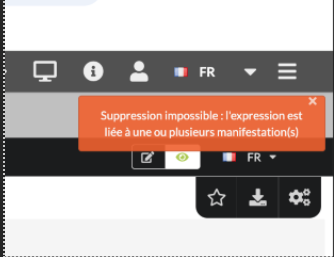
\includegraphics[width=0.7\textwidth]{images/terminologie.png} 
	
	\caption{Message de suppression d'une notice d'\gls{oeuvre}} 
	
	\label{figterminologie} 
	
\end{figure}

Cette proposition rejoint l’idée de supprimer la table œuvre cinématographique dans la gestion des masques alors que c’est la table œuvre/expression qui est couramment utilisée.  

Enfin, une confusion peut également s’installer entre les termes “œuvre liée” et “œuvre associée” dans les masques qui décrivent la \gls{manifestation} par exemple. Le terme d’œuvre liée pourrait être corrigé en “œuvre parente” pour que la nature du lien soit plus claire entre les deux entités.  

%\subsection{Conserver le niveau du FRBR en mode saisie sur les métas masques }
%
%Actuellement, lors de la configuration des méta-masques, les champs glissés et déposés dans le type de notice concernée perdent la mention du niveau FRBR auquel ils appartiennent. L’utilisateur n’a plus le moyen de savoir, une fois dans la notice, que tel champ appartient à tel niveau. Conserver la mention du niveau du FRBR sur les métas masques au sein de la saisie de la notice permettrait une meilleure compréhension et visibilité pour l’utilisateur. Ainsi, par exemple, dans une notice de \gls{manifestation}, le champ Titre afficherait : Œuvre – Titre.  

\section{Nouvelles fonctionnalités }

\subsection{Annotation de séquences sur un fichier vidéo numérique }

La table média actuelle permet seulement de visualiser une photo ou une vidéo, au clic sur la notice. Toutefois, il serait intéressant de développer une visionneuse spécifique à la vidéo qui permettrait non seulement de la visionner, mais également d’y placer des repères, des marqueurs, et de pouvoir l’annoter.  

Tout d’abord, deux possibilités de “séquençage” manuel seraient possibles :  

\begin{itemize}
	\item L’utilisateur saisit des repères temporels sur la vidéo sans la modifier. Ces repères sont reversés dans des champs prévus pour accueillir les “time codes” dans la notice de l’objet numérique. À l’ouverture du fichier numérique, les marqueurs laissés par l’utilisateur apparaissent, visibles sur la barre de défilement de la vidéo. L’utilisateur peut alors cliquer sur ces marqueurs pour naviguer au sein de la vidéo comme il le souhaite, et y voir les annotations associées.  
	
	\item L’utilisateur pourrait aussi vouloir segmenter le fichier vidéo en plusieurs séquences distinctes à partir de time codes précis. Dans ce cas-là, à la manière d’un logiciel de montage, l’utilisateur peut créer des cuts sur la vidéo et ainsi créer plusieurs fichiers numériques à partir de celle-ci, mais qui lui sont toujours liés. En effet, ces nouveaux objets, fragments du fichier vidéo d’origine, auraient leur propre notice de description mais resteraient rattachés à la notice principale, à la manière d’un ensemble.  
\end{itemize}

Cette nouvelle fonctionnalité permettrait d’apprécier l’hétérogénéité des collections, et s’avèrerait utile dans le cas, par exemple, de rushes documentaires non édités que l’utilisateur souhaiterait diviser par mots clés ou thématiques. La description des médias vidéo n’en serait que plus affinée et précisée.  

Par ailleurs, ce séquençage devra être effectué dans une optique d’annotation “sur” l’image, permettant ainsi d’associer des séquences plus précises à une description thématique. Concrètement, deux cas d’annotation sont possibles :  

\begin{itemize}
	\item L’utilisateur pourrait être capable de placer des tags sur des éléments de l’image (objets, personnes, éléments techniques, contenu...) et d’en décrire le contenu dans les champs prévus. La notice du média prévoit alors l’affichage d’une description par time codes, sur lesquels l’utilisateur peut cliquer pour accéder directement à l'image en question.  
	
	\item L’utilisateur peut également vouloir décrire une séquence dans sa globalité, à l’intérieur d’un time code précis. Dans ce cas, les champs sont saisis à partir d’un tag sur le time code, et non plus sur un élément précis de l’image.  L’affichage de la description dans la notice peut rester le même que le précédent.  
\end{itemize}


À l’ouverture du fichier vidéo, les annotations saisies apparaissent à droite de la visionneuse, et les times codes superposés à la barre de défilement de la vidéo.  

La description précise sur des séquences vidéo permettrait à la recherche d’être plus performante : l’utilisateur pourrait, en cherchant certains mots clés, tomber directement sur les séquences numériques associées, aux time codes correspondants. 

Il est intéressant de penser également à la mise en place d’une recherche par mots clés au sein du fichier numérique vidéo. La recherche d’un mot clé amène l’utilisateur à une séquence décrite par ce mot clé.   


\subsection{ \label{graphe}Mise en place d’une visualisation des liens entre entités du FRBR }

Cette idée s’inspire visuellement de la “balade intuitive” proposée par la bibliothèque Kandinsky dont voici un exemple :

\begin{figure}[htbp] 
	
	\centering 
	
	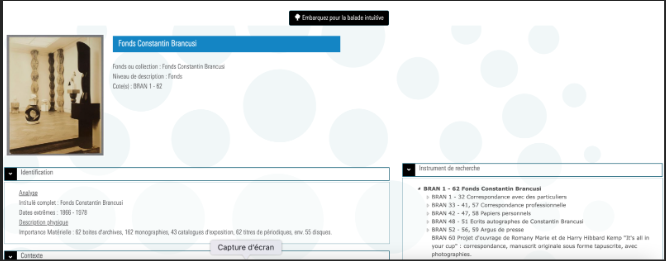
\includegraphics[width=1.0\textwidth]{images/kandinsky1.png} 
	
	\caption{Vue "balade intuitive" proposée par la bibliothèque Kandinsky \footcite{zotero-item-801}} 
	
	\label{figkandinsky1} 
	
\end{figure}

\begin{figure}[htbp] 
	
	\centering 
	
	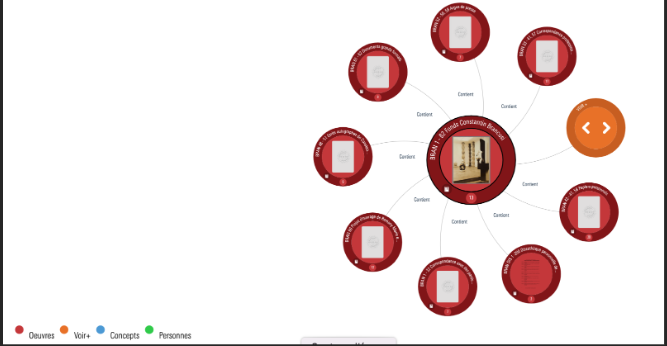
\includegraphics[width=1.0\textwidth]{images/kandinsky2.png} 
	
	\caption{Vue en graphe de la balade intuitive \footcite{zotero-item-801}} 
	
	\label{figkandinsky2} 
	
\end{figure}

Lorsque l’utilisateur ouvre S-Movies, ce sont les œuvres qui apparaissent sous la forme de résultats de recherche. Les liens avec d’autres notices (\gls{manifestation}s et \gls{item}s) n’apparaissent pas à première vue. Il faut ouvrir une notice pour voir la liste des entités qui y sont liées, si toutefois ces liens sont configurés dans le menu de la notice. Or, la visualisation de liens entre les entités d’une collection est primordiale dans la logique d’une structuration selon le modèle FRBR. Pouvoir avoir un aperçu de ces liens pourrait améliorer la compréhension de la hiérarchie entre les niveaux du FRBR et leur délimitation, et ainsi améliorer les pratiques de saisie selon les cas d’indexation. De plus, visualiser rapidement les liens entre entités permettrait d’identifier les incohérences et les erreurs de données plus facilement, comme par exemple, des éléments vides ou isolés. 

Les entités principales du FRBR étant au nombre de trois, la représentation choisie pourrait être celle d’une représentation en graphes de connaissances, modélisant ainsi les relations entre entités. Cette représentation s’appuie sur le modèle de graphe RDF (sujet-prédicat-objet) qui permet également l’interopérabilité des données.  

Pour penser la place que pourrait prendre cette visualisation des liens dans l’application, il faut se poser les questions suivantes : quel niveau du FRBR les utilisateurs préfèrent-ils visualiser ? Dans quel contexte ? Autrement dit, il faut se demander quel niveau de granularité choisir pour mettre en place cette visualisation et à quel endroit de l’application. 

Puisque la page d’accueil de l’espace de travail S-Movies présente les œuvres, la représentation en graphe pourrait dans un premier temps permettre de visualiser les œuvres présentes dans la collection.  

Le premier niveau permettrait donc à l’utilisateur de visualiser la liste des œuvres préservées sous formes de cercles, plus ou moins gros selon le nombre de sous-niveaux qu’elles contiennent. Ainsi, une œuvre qui contiendrait deux \gls{variante}s, quatre \gls{manifestation}s, 12 \gls{item}s sera plus grande qu’une \gls{oeuvre} qui contient 1 \gls{manifestation} et 1 \gls{item}.  

Au clic sur l’\gls{oeuvre}, le détail de ses relations avec des sous-éléments apparait : \gls{variante}s, \gls{manifestation}s, \gls{item}s.  

Ce mode d’affichage pourrait être disponible de la même manière que les modes d’affichage déjà présents dans l’application. Il faudrait ajouter un mode d’affichage en “graphe”. 

\begin{figure}[htbp] 
	
	\centering 
	
	
\includegraphics[width=0.6\textwidth]{images/vue.png} 
	
	\caption{Modes d'affichage disponibles dans l'application} 
	
	\label{figvues} 
	
\end{figure}

Ce mode d’affichage, établit au niveau des tables, pourrait également être disponible au niveau des notices. Par exemple dans une notice d’\gls{item}, un onglet de menu pourrait être configurable pour faire apparaitre, en graphe, les relations de l’\gls{item} avec les niveaux parents du \gls{FRBR}.   

Il serait intéressant d’intégrer à ces visualisations en graphes les médias, d’autant plus dans le cas de la mise en place d’une segmentation vidéo, pour pouvoir visualiser les différents segments reliés à l’\gls{item}.  

Concrètement, le parcours utilisateur de cet affichage serait le suivant :   
\begin{itemize}
	\item Que ce soit depuis une table ou depuis une notice, l’utilisateur clique sur le mode d’affichage en graphe  
	
	\item Les entités concernées s’affichent sous la forme de cercles, proportionnels aux nombres de liens qu’ils entretiennent avec les autres niveaux du \gls{FRBR}. Les cercles comportent des informations minimales selon le niveau : le titre et la date pour les œuvres, le titre le format et la date pour les \gls{manifestation}s, le titre, le format, la date et l’identifiant pour l’\gls{item}. 
	
	\item Une légende s’affiche en bas de l’écran avec un code couleur pour chaque entité, et le nombre d’entités présentes.  
	
	\item Au clic de l’utilisateur sur l’un des cercles, le détail des relations de l’entité avec d’autres entités s’ouvre en mode graphe. Le résumé de la notice s’affiche en barre latérale sur le côté.  
	
	\item Au clic sur une entité liée, le graphe se reforme et l’entité choisie devient le centre du graphe.  
\end{itemize}


On pourrait également ajouter au graphe les lieux et les personnes (intervenants) liés à chaque entité du \gls{FRBR}. 



\chapter{\label{annexe_B}Spécification fonctionnelle : Recherche en langage naturel à l’appui de l’intelligence artificielle } 
\titreEntete{Specification fonctionnelle}

Cette seconde annexe, présente une spécification fonctionnelle pour la mise en place d'un outil de recherche en langage naturel, fondé sur l'intelligence artificielle, rédigée à la demande de Skinsoft dans le cadre de notre stage. Cet outil est actuellement en cours de développement. L'implémentation de la recherche en langage naturel a fait l'objet de recherches et de réflexions parallèles à celles de la segmentation et de l'indexation automatisées. Le document est structuré en deux parties : les principes d'usage théoriques, la spécification fonctionnelle détaillée à l'appui de maquettes visuelles. 

Cette spécification a été rédigée conjointement avec Florian Martin, également stagiaire chez Skinsoft.
Réduite pour les besoins de notre étude, cette annexe fait en réalité partie d'une spécification plus large rendue avec ce mémoire comme livrable technique. 

\section{Le besoin utilisateur}

L’application doit proposer un mode de recherche alternatif à la recherche simple, basé sur l’intelligence artificielle. Cela doit permettre de questionner l’application en langage naturel dans un double objectif :  

Rendre chaque table interrogeable sans utilisation de vocabulaire contrôlé ou de la recherche avancée : une simple phrase suffit 

Par exemple : 

\begin{itemize}
	\item “Tous les films réalisés par David Lynch en 1987” 
	
	\item “Tous les films numériques” 
	
	\item “Toutes les photos au format dng” 
\end{itemize} 

Agir comme un générateur de requête exécutable par l’utilisateur sur la table interrogée ET la recherche fédérée.  

\section{Principes d'usage}

\subsection{Mode de "recherche augmentée" alternatif \label{infobulle}}

Dans les outils de recherche, à côté de la barre de recherche je clique sur le bouton de recherche augmentée. La barre de recherche passe de la fonctionnalité “recherche simple” à la “recherche augmentée” : on peut interroger la table en question à l’aide de phrases.  

Il y a une distinction visuelle établie dès le clic :  

\begin{itemize}
	\item Le fond du bouton se colorie selon la couleur de l’interface définie dans la notice d’établissement. Fonctionnement actuel des autres boutons 
	
	\item Apparition d’un symbole warning dans la barre de recherche, à son extrémité droite. Au survol avec la souris, une infobulle s’ouvre avec le message : “Recherche augmentée activée, vous utilisez l’intelligence artificielle. Fonctionnalité limitée à l’usage des données existantes.”  
\end{itemize}


Changement du message inscrit dans la barre de recherche :  

\begin{itemize}
	\item Recherche simple : “Recherche” 

	\item Recherche augmentée : “Interrogez-moi”
\end{itemize}  

\subsection{Gestions des erreurs}

Deux logiques : 

\begin{itemize}
	\item La possibilité pour le processus d’indiquer qu’il ne comprend pas la requête utilisateur afin d’éviter la création d’une requête erronée. 
	\item La possibilité pour l’utilisateur de signaler un problème. 

\end{itemize}

En cas d’incompréhension de la requête utilisateur et d’incertitude sur la requête à générer. La fonctionnalité doit :  

\begin{itemize}
	\item Ne pas lancer la requête car il n’est pas certain.  

	\item Identifier le point bloquant  

	\item Signaler l’erreur par un code couleur : 
	
	\subitem Le mot posant un problème est surligné en rouge lorsque incompréhension totale. 
	
	\subitem Le mot pose un problème est surligné en orange lorsqu’il y a une incertitude sur le sens. 
	
\end{itemize}


L’utilisateur doit pouvoir écrire dans la barre de recherche un complément à la requête d’origine. 

\begin{itemize}
	\item Le complément s’envoie au processus comme une requête classique. C’est l’interprétation qui change.  

	\item S'il y a toujours une erreur, on revient à l’étape précédente jusqu’à résolution de l’erreur.  

	\item Si l’utilisateur tombe dans une boucle infinie et décide d’arrêter le traitement, l’absence d’activité dans la barre de recherche dans les 30 secondes met fin au processus.  

	\item Si le complément amène à résoudre l’erreur, le processus suit son cours. 
\end{itemize}



En cas d’une requête générée mais invalide selon l’utilisateur, ce dernier peut la reporter afin que le modèle enregistre l’incident, comprenne l’erreur et s’affine. 

À côté du résumé se trouve un bouton “Reporter une erreur”  

Au clic sur le bouton, ouverture d’un formulaire afin de reporter une erreur. S’ouvre comme une notice. 

Quatre champs sont affichés :  

\begin{itemize}
	\item Champ Titre du rapport : l’utilisateur saisi un titre pour le rapport d’erreur. Permet de le rendre traçable. 

	\item Champ requêtes : rempli automatiquement, il contient la requête utilisateur (la phrase de départ) + le résumé de la recherche générée par IA. Non visible par l’utilisateur, y figure aussi la requête ElasticSearch générée.  

	\item Champ date : rempli automatiquement avec le jour de requêtage 

	\item Champ description : l’utilisateur explique pourquoi cela ne lui convient pas et ce qu’il attendait.  
\end{itemize}



Deux boutons sont disponibles :  

\begin{itemize}
	\item “Envoyer” : 
	\subitem Envoie le rapport d’incident au LLM, l’historise et l’intègre dans une base de données pour entraînement. 

	\subitem Génère une notification verte à l’endroit habituel : “Rapport d’erreur envoyé et enregistré”. 

	\item “Annuler” : Annule l’opération en cours. 

	\subitem Génère une notification orange à l’endroit habituel : “Rapport d’erreur annulé”. 
\end{itemize}



\section{Fonctionnalité détaillée}

\subsection{Infobulle}

Au survol de la souris, le symbole affiche une infobulle contenant un court message qui informe l’utilisateur de l’utilité de la recherche activée. Le symbole est affiché en tout temps lorsque la recherche augmentée est activée. 

\begin{figure}[htbp] 
	
	\centering 
	
	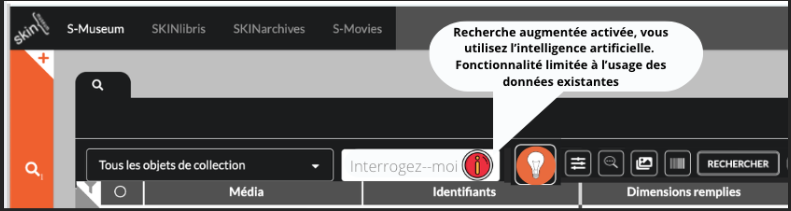
\includegraphics[width=1.0\textwidth]{images/infobulle.png} 
	
	\caption{Infobulle d'activation} 
	
	\label{figinfobulle} 
	
\end{figure}

\subsection{Requête mal formulée ou incertaine}

Si la requête de l’utilisateur est mal formulée ou incorrecte, empêchant la recherche augmentée d’être lancée, deux options sont possibles.  

Si l’outil est incertain quant à l’interprétation d’un terme utilisé dans la requête, celui-ci est surligné en couleur orange :  

\begin{figure}[htbp] 
	
	\centering 
	
	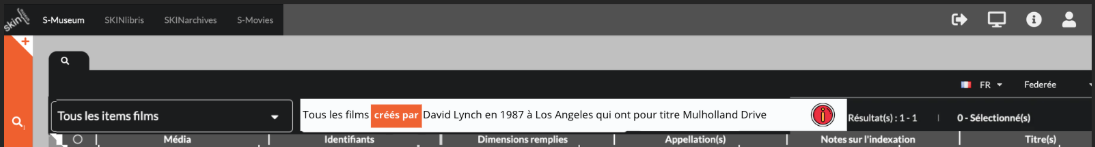
\includegraphics[width=1.0\textwidth]{images/annexe1.png} 
	
	\caption{Incertitude quant au terme utilisé} 
	
	\label{figincertitude} 
	
\end{figure}

Si l’outil ne comprend pas la requête, parce qu’elle est incohérente ou inadaptée, celle-ci est surlignée en rouge :  

\begin{figure}[htbp] 
	
	\centering 
	
	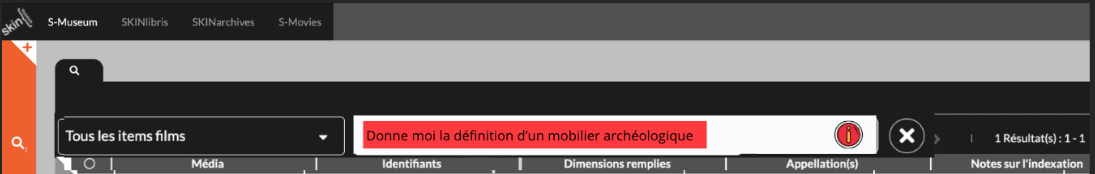
\includegraphics[width=1.0\textwidth]{images/annexe2.png} 
	
	\caption{Incohérence du terme utilisé} 
	
	\label{figIncoherence} 
	
\end{figure}

\subsection{Résultats de recherche invalides :}

Si les résultats de recherche retournés par la recherche augmentée sont erronés selon l’utilisateur, et ne correspondent pas à la requête qui a été formulée, il peut signaler l’incident dans un formulaire prévu à cet effet, via un bouton “reporter un problème” dans l’onglet de résumé : 

\begin{figure}[htbp] 
	
	\centering 
	
	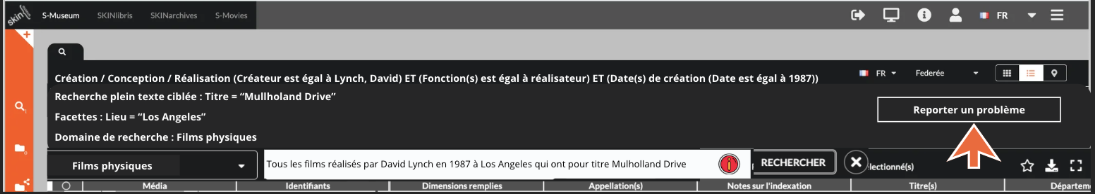
\includegraphics[width=1.0\textwidth]{images/annexe3.png} 
	
	\caption{Reporter un problème} 
	
	\label{figReporteunPb} 
	
\end{figure}

Au clic sur ce bouton, un formulaire s’ouvre sous la forme d’une notice que l’utilisateur peut remplir pour décrire le problème détecté. Les champs “date” (format calendaire) et “requête effectuée” sont automatiquement remplis :  

\begin{figure}[htbp] 
	
	\centering 
	
	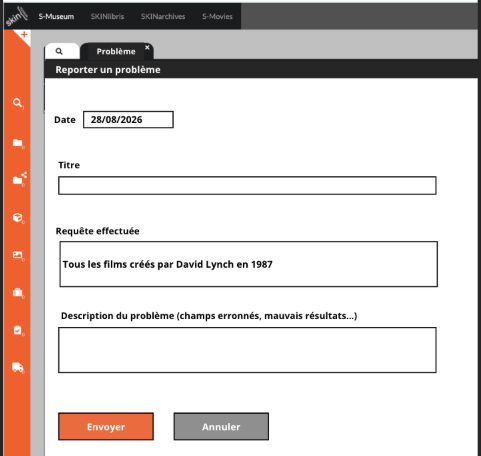
\includegraphics[width=1.0\textwidth]{images/annexe4.png} 
	
	\caption{Formulaire d'erreur} 
	
	\label{figFormulaire} 
	
\end{figure}

Au clic sur “envoyer”, un message de validation apparait :  

\begin{figure}[htbp] 
	
	\centering 
	
	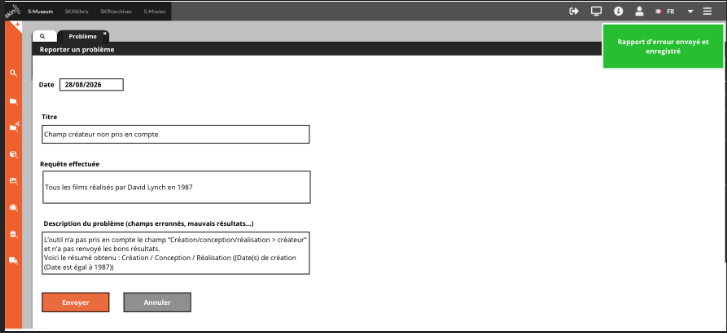
\includegraphics[width=1.0\textwidth]{images/annexe5.png} 
	
	\caption{Message de validation} 
	
	\label{figValidation} 
	
\end{figure}

\newpage{\pagestyle{empty}\cleardoublepage}

%%%%%%%%%%%%%%%%%%

\backmatter % glossaire, index, table des figures, table des matières.. (la bibliographie a déjà été appelée)

%\printindex
%\glsaddall
\printglossary[title=Glossaire]
\printglossary[type=\acronymtype, title={Liste des abréviations}]
\listoftables
\listoffigures
\tableofcontents
\end{document}
